\documentclass{article}
\usepackage{graphicx} % Required for inserting images

\title{Chapter 2: On Monitoring Compliance for Open-Ended Two Agent Contracts }
\author{kharrazkaram }
\date{September 2025}
\usepackage{subcaption}
\usepackage{float}
\usepackage{placeins}
% Relax float placement rules globally
\renewcommand{\topfraction}{0.95}
\renewcommand{\floatpagefraction}{0.85}
\usepackage{pdflscape}
\usepackage{xspace}
\usepackage{paralist}
\DeclareMathAlphabet{\mathcal}{OMS}{cmsy}{m}{n}
%\usepackage{inparaenum}
\newcommand{\defn}[1]{\emph{#1}}
\newcommand{\PAY}{\ensuremath{\mathsf{PAY\_R}}\xspace}
\newcommand{\PAYF}{\ensuremath{\mathsf{PAY\_F}}\xspace}
\newcommand{\notifrepair}{\ensuremath{\mathsf{Notif\_R}}}   % tenant repair request (notification)
\newcommand{\notifterm}{\ensuremath{\mathsf{Notif\_T}}}         % tenant termination notice
\newcommand{\REPAIR}{\ensuremath{\mathsf{Maint\_P}}}
\newcommand{\OCC}{\ensuremath{\mathsf{OCC}}\xspace}
%\newcommand{\OCC}{\ensuremath{\mathsf{OCC}}\xspace}
\newcommand{\occ}[1]{\OCC^{(#1)}}
\newcommand{\pay}[1]{\PAY^{(#1)}}
\newcommand{\payf}[1]{\PAYF^{(#1)}}
 \newcommand{\Cpayp}[1]{\PAY_{#1}^{+}}
 \newcommand{\Cpaym}[1]{\PAY_{#1}^{-}}
 \newcommand{\Coccp}[1]{\OCC_{#1}^{+}}
 \newcommand{\Coccm}[1]{\OCC_{#1}^{-}}
 \newcommand{\SigA}[1]{\Sigma^{A}_{#1}} % active-participation (enablers)
 \newcommand{\SigI}[1]{\Sigma^{I}_{#1}} % interference (blockers)
\newcommand{\Wordsfin}[1]{#1^{*}}
\newcommand{\Wordsinf}[1]{#1^{\omega}}
\newcommand{\Words}[1]{#1^{\le\omega}} % = finite or infinite
\newcommand{\acta}{\ensuremath{\mathsf{a} \xspace} }
\newcommand{\Undef}{{\ensuremath{\mathsf{undefined}}\xspace}}
% Trace meta-notation
\newcommand{\Tr}[1]{\ensuremath{\mathsf{Tr}(#1)}}
\newcommand{\pos}[2]{\ensuremath{\mathsf{pos}(#1,#2)}}
\newcommand{\Live}{\mathsf{Live}}
\newcommand{\Pref}{\mathsf{Pref}}
\providecommand{\Prog}{\ensuremath{\mathsf{Prog}}\xspace}
\newcommand{\llangle}{\langle\!\langle}
\newcommand{\rrangle}{\rangle\!\rangle}
\newcommand{\trig}[2][]{\llangle #1 \rrangle #2 }

\newcommand{\concat}{\circ}
% Macros for constructs (put in preamble)
\newcommand{\obl}[2][]{\mathbf{O}_{#1}(#2)}        % obligation
\newcommand{\frb}[2][]{\mathbf{F}_{#1}(#2)}        % prohibition
\newcommand{\perm}[2][]{\mathbf{P}_{#1}(#2)}        % permission
\newcommand{\repit}[1]{\mathbf{Rep}(#1)}             % repetition
\newcommand{\guard}[2][]{\lceil #1 \rceil #2 }   % guard
\newcommand{\repair}{\blacktriangleright}          % choice operator
       
\newcommand{\strat}{\mathfrak{S}}
\newcommand{\unlab}{\mathsf{unlab}}
\newcommand{\unlabone}{\mathsf{unlab}_1}
\newcommand{\unlabtwo}{\mathsf{unlab}_2}
%\newcommand{\emptytrace}{\varepsilon}
\newcommand{\Sig}[1]{\Sigma_{#1}}
\newcommand{\taumt}{\tau^{\mathrm{mt}}}           % metric-timed word symbol
\newcommand{\Ik}[1]{I_{#1}}                        % interval I_k
\newcommand{\Aik}[2]{A^{(#1)}_{#2}}                % A^{(i)}_k
\newcommand{\AggI}{\mathsf{Agg}_{I}}               % aggregation operator Agg_I
\newcommand{\wordsets}[1]{(2^{#1})} 
\newcommand{\trace}[1]{\ensuremath{\langle #1 \rangle \xspace}}
\newcommand{\emptytrace}{\ensuremath{\trace{-}}}
\newcommand{\emptc}{\ensuremath{\epsilon_{C}}}
%\newcommand{\defn}{\emph}
\newcommand{\shuffle}{\mathbin{|\!|\!|}}
%\newcommand{\taumt}{\tau^{\mathrm{mt}}}
\newcommand{\tault}{\tau^{\mathrm{lt}}}
\newcommand{\taust}{\tau^{\mathrm{st}}}
\newcommand{\LT}{\ensuremath{\mathsf{LT}}}
\newcommand{\erase}{\ensuremath{\mathsf{erase}}}
\newcommand{\ST}{\ensuremath{\mathsf{ST}}}
% \newcommand{\obl}{O}
% \newcommand{\frb}{F}
% \newcommand{\perm}{P}
\newcommand\bydef[1]{\xLeftrightarrow{\text{#1}}}
\newcommand\cDLunmath{c\mathcal{DL}\xspace}
%\newcommand{\badclass}[1]{\mathrm{BPL}(#1)}\
\newcommand\cDL{\ensuremath{\logic{TACNL}} \xspace}
\newcommand\cdl{\cDL}
\newcommand{\andd}{~\text{and}~}
\newcommand{\Rej}{\textit{Rej}}
\newcommand{\Acc}{\textit{Acc}}
\newcommand\mydef{\mathrel{\overset{\makebox[0pt]{\mbox{\normalfont\tiny\sffamily def}}}{=}}}
\newcommand\sat{\models_{\top}}
\newcommand\viol{\models_{\perp}}
\newcommand\satt{\models_{\topt}}
\newcommand\violt{\models_{\bott}}

\newcommand{\presat}{\models_{?}}
\newcommand{\clossat}{\models_{Cl}}

\newcommand{\postsat}{\models_{\topp}}
\newcommand{\postviol}{\models_{\botp}}

\newcommand\qsat{\models_{Q,\top}^p}
\newcommand\qsatv{\models_{Q,\bot}^p}
\newcommand\qsatun{\models_{Q,?}^p}
\newcommand\qsatt[1]{\models_{Q}^#1}
\newcommand\score{\rho}
%newcommand\guard{\rotatebox[origin=c]{-90}{$\bumpeq$}}
\newcommand{\sequence}[1]{\ensuremath{\langle #1 \rangle}}
\newcommand\trans{\tau}
\newcommand\vtrans{\bar{\tau}}
\newcommand{\tool}[1]{\ensuremath{\textsl{#1}}\xspace}
\newcommand{\monadop}[3]{\tool{#1}^{#2}(#3)}
\newcommand{\dyadop}[5]{\tool{#1}^{#2}(#3\mid^{#4} #5)}
\newcommand{\dyadopa}[5]{\tool{#1}^{#2}(#3~\|^{#4} #5)}
\newcommand{\dop}{\tool{dop}}
\newcommand{\mt}[1]{$#1$}
\newcommand{\dotcup}{\mathbin{\dot\cup}}

\newcommand{\topt}{\top^t}
\newcommand{\bott}{\bot^t}
\newcommand{\topp}{\top^p}
\newcommand{\botp}{\bot^p}
\newcommand{\bottp}[1]{\mathbin{\bot^{t}_{#1}}} 
\newcommand{\botpp}[1]{\mathbin{\bot^{p}_{#1}}}
\newcommand{\bottone}{\bottp{1}}
\newcommand{\botttwo}{\bottp{2}}
\newcommand{\botttwelve}{\bottp{1,2}}



\newcommand{\BindFiveRegions}[1]{%
  \begingroup
  \def\Llocal{#1}%
  \xdef\PreDef{\noexpand\Pre{\Llocal} := \noexpand\closureclass{\noexpand\minlang{\Llocal}}\setminus \noexpand\minlang{\Llocal}}%
  \xdef\EADef{\noexpand\EAL{\Llocal} := \noexpand\minlang{\Llocal}}%
  \xdef\ERDef{\noexpand\ERL{\Llocal} := \noexpand\sbad{\Llocal}}%
  \endgroup
}
% (Use text to state the equalities; LaTeX macro assignment of sets is for readability.)

% --- Five-valued semantics bracket ---
\newcommand{\semfive}[1]{\left\llbracket #1 \right\rrbracket_{5}}
\newcommand{\qsem}[1]{\left\llbracket #1 \right\rrbracket_{\text{qviol}}}
\newcommand{\qblame}[1]{\left\llbracket #1 \right\rrbracket_{\text{qblame}}}

\newcommand{\Pre}[1]{\mathsf{Pre}\!\left(#1\right)}   % pre-eager verdict
\newcommand{\EAL}[1]{\mathsf{EA}\!\left(#1\right)}    % eager acceptance
\newcommand{\ERL}[1]{\mathsf{ER}\!\left(#1\right)}    % eager rejection
\newcommand{\IALs}[1]{\IAL{#1}}                        % irrelevant acceptance (already defined)
\newcommand{\IRLs}[1]{\IRL{#1}}     
%duty relation
\newcommand{\dutysat}{\ensuremath{\vDash_D }\xspace}
%right relation
\newcommand{\rightsat}{\ensuremath{\vDash_R}\xspace}
%pointed violation
\newcommand{\dutyviol}{\ensuremath{\nvDash_D}\xspace}
%duty violation
\newcommand{\minviol}{\vDash_D^{\tool{viol}}}
%pointed satisfaction
\newcommand{\minsat}{\vDash_D^{\tool{sat}}}
%if mathmode
\newcommand{\ift}{\text{if \xspace}}
%then mathmode
\newcommand{\thent}{\text{ then \xspace}}
%else mathmode
\newcommand{\elset}{\text{ else \xspace}}
%generic monad obligation 
\newcommand{\monadob}{\ensuremath{\monadop{O}{\is}{a}}}
%generic monad prohibition 
\newcommand{\monadf}{\ensuremath{\monadop{F}{\is}{a}}}
%generic monad strict permission
\newcommand{\monadsp}{\ensuremath{\monadop{SP}{\is}{a}}}
%generic monad obligation permission
\newcommand{\monadp}{\ensuremath{\monadop{P}{\is}{a}}}
%generic absolute dyadic obligation 
\newcommand{\abdyadob}{\ensuremath{\dyadopa{O}{\is}{a}{R}{b}}}
%generic absolute dyadic prohibition
\newcommand{\abdyadf}{\ensuremath{\dyadopa{F}{\is}{a}{R}{b}}}
%generic absolute dyadic strict obligation
\newcommand{\abdyadsp}{\ensuremath{\dyadopa{SP}{\is}{a}{R}{b}}}
%generic absolute dyadic permission
\newcommand{\abdyadp}{\ensuremath{\dyadopa{P}{\is}{a}{R}{b}}}


\newcommand{\timedevents}{\ensuremath{\Sigma \times \mathbb{N}}}
\newcommand{\timedist}{\ensuremath{\mathsf{tdist}}}


%generic relative dyadic obligation 
\newcommand{\dyadob}{\ensuremath{\dyadop{O}{\is}{a}{R}{b}}}
%generic relative dyadic prohibition
\newcommand{\dyadf}{\ensuremath{\dyadop{F}{\is}{a}{R}{b}}}
%generic relative dyadic strict obligation
\newcommand{\dyadsp}{\ensuremath{\dyadop{SP}{\is}{a}{R}{b}}}
%generic relative dyadic permission
\newcommand{\dyadp}{\ensuremath{\dyadop{P}{\is}{a}{R}{b}}}
\newcommand{\phid}{\ensuremath{\phi_d}}
\newcommand{\phir}{\ensuremath{\phi_r}}

\newcommand{\DOP}[1]{\ensuremath{\norm{DOP}}_#1}
\newcommand{\nc}{\norm{NC}}
\newcommand{\ns}{\norm{NS}}
\newcommand{\NS}{\mathcal{NS}}
\newcommand{\size}[1]{\vert #1\vert}
\newcommand{\n}{\norm{N}}
\newcommand{\oplusl}{\vec{\oplus}}
\newcommand{\tmin}{t_{min}}
\newcommand{\tmax}{t_{max}}
\newcommand{\occisarg}[2]{\ensuremath{\mathsf{tp}(w,#1,#2)}}
\newcommand{\occisa}{\ensuremath{\mathsf{tp}(w,\is,a)}}
\newcommand{\mtp}{\ensuremath{\mathsf{mtp}}}
\newcommand{\cl}{\ensuremath{\mathsf{Cl}}}
\newcommand{\mtpa}{\ensuremath{\mathsf{mtp}(w,\is,a)}}
\newcommand{\mtpb}{\ensuremath{\mathsf{mtp}(w,\is,b)}}
\newcommand{\occis}{\ensuremath{\mathsf{tp}}}
\newcommand{\occisb}{\ensuremath{\mathsf{tp}(w,\is,b)}}
\newcommand{\pref}{\ensuremath{\mathsf{pre}}}
\newcommand{\DC}{\ensuremath{\mathsf{NC}}}
\newcommand{\suff}{\ensuremath{\mathsf{suf}}}
\newcommand{\ntd}{\ensuremath{\mathsf{NTD}}}
\newcommand{\synth}{\ensuremath{\mathsf{synthetize}}}
\newcommand{\tcst}{\ensuremath{\mathsf{Tcstr}}}
\newcommand{\psts}{\ensuremath{\mathsf{psts}}}
\newcommand{\maxpush}{\ensuremath{\union^{m}}}
\newcommand{\cst}{\ensuremath{\mathsf{cstr}}}
\newcommand{\cstp}{\ensuremath{\mathsf{CstrC}}}
\newcommand{\remin}{\ensuremath{\mathsf{rem}}}
% \newcommand{\bottp}[1]{\mathbin{\bot^{t}_{#1}}}    % tight violation blamed on agent set #1 ∈ {1,2,1,2}
% \newcommand{\botpp}[1]{\mathbin{\bot^{p}_{#1}}}    % post violation blamed on agent set #1
\newcommand{\barp}{\overline{p}}    

\newcommand{\opx}{\ensuremath{~\mathsf{op}}~}
\newcommand{\bad}{\ensuremath{\mathsf{Mbad}}}
\newcommand{\tblamemon}{\ensuremath{\mathcal{M}_{11}}}
\newcommand{\tmon}{\ensuremath{\mathcal{M}^{TS}}}
\newcommand{\tsmc}{\ensuremath{\mathsf{TSMC}}}
\newcommand{\regmon}{\ensuremath{\mathsf{RTM}}}
\newcommand{\occisam}{\ensuremath{w_{min}(\is,a)}}
\newcommand{\inset}{\bigvee_{I \in \is} I}
\newcommand{\gpre}{\ensuremath{\mathsf{gpre}(w,\nc) \xspace}\xspace}
\newcommand{\bpre}{\ensuremath{\mathsf{bpre}(w,\nc) \xspace}\xspace}
\newcommand{\gprearg}[1]{\ensuremath{\mathsf{gpre}(w,#1) \xspace}}
\newcommand{\bprearg}[1]{\ensuremath{\mathsf{bpre}(w,#1) \xspace}}
\newcommand{\usat}{\ensuremath{\mathsf{U-sat} \xspace}}
\newcommand{\satext}{\ensuremath{\mathsf{sat} \xspace}}
\newcommand{\unsat}{\ensuremath{\mathsf{unsat} \xspace}}
\newcommand{\mintau}{\tau_{min}}
\newcommand{\tNFA}{\ensuremath{\mathsf{2NFA}}\xspace}
% Automata macros (inserted if not already defined)
\newcommand{\NFA}{\ensuremath{\mathsf{NFA}}\xspace}
\newcommand{\DFA}{\ensuremath{\mathsf{DFA}}\xspace}
\newcommand{\aut}{\ensuremath{\mathcal{A}}\xspace}
\newcommand{\autre}{\ensuremath{\mathsf{A}_{re}}\xspace}
\newcommand{\autrep}{\ensuremath{\mathsf{A}_{re}}\xspace}
\newcommand{\autrec}[1]{\ensuremath{\mathsf{A}_{#1}}\xspace}
\newcommand{\primdos}{{\prime\prime}}
\newcommand{\trigg}{\text{trig}}
\newcommand{\guardd}{\text{guard}}
\newcommand{\nrep}{\text{frep}}
\newcommand{\omga}{\ensuremath{\omega}}
%Logics
\newcommand{\logic}[1]{\ensuremath{\mathsf{#1}}\xspace}
\newcommand{\TDDL}{\logic{MTNL}}
\newcommand{\LTL}{\logic{LTL}}
\newcommand{\LDL}{\logic{LDL}}
\newcommand{\CTL}{\logic{CTL}}
\newcommand{\DL}{\logic{DL}}
\newcommand{\STIT}{\logic{STIT}}
\newcommand{\TDDLfm}{\logic{FMMTNL}}
\newcommand{\TDDLm}{\ensuremath{\logic{MTNL^{m}}~}}
\newcommand{\IO}{\logic{I/O Logic}}
\newcommand{\DDL}{{\ensuremath{\mathsf{DDL}}}\xspace}
\newcommand{\CTD}{{\ensuremath{\mathsf{CTD}}}\xspace} 
%norms
\newcommand{\tightverdicts}{\ensuremath{\mathbb{V}_5} \xspace}

%bad language
%\newcommand{\badclass}[1]{\llbracket #1 \rrbracket_{BL}}
% === Core symbols ===
\newcommand{\re}{\ensuremath{\mathsf{re}}}
\newcommand{\modelsre}{\ensuremath{\models_{\re}}}

% === Language-of (for a regexp or an automaton) ===
% Use \Lang(\cdot) for "language of ...", avoid \lang vs \class collision.
\newcommand{\Lang}[1]{\mathcal{L}\!\left(#1\right)}

% === Language operators on sets of words ===
% Prefix-closure and bad-prefix
\newcommand{\closureclass}[1]{\operatorname{\mathsf{PCl}}\!\left(#1\right)}
\newcommand{\badclass}[1]{\operatorname{\mathsf{BP}}\!\left(#1\right)} % Bad Prefix language

\newcommand{\ECl}{\mathrm{ECl}}

% Minimal elements of a language
\newcommand{\minlang}[1]{\operatorname{\mathsf{Min}}\!\left(#1\right)}

% Three derived regions (make them proper operators with 1 arg)
\newcommand{\IAL}[1]{\operatorname{\mathsf{IAL}}\!\left(#1\right)} % Irrelevant Acceptance Language
\newcommand{\sbad}[1]{\operatorname{\mathsf{SBad}}\!\left(#1\right)} % Strict Bad frontier
\newcommand{\IRL}[1]{\operatorname{\mathsf{IRL}}\!\left(#1\right)} % Irrelevant Rejection Language

% Complement of a set (works for languages too)
\newcommand{\cclass}[1]{\overline{#1}}

% === Automaton builders (keep separate from language operators) ===
\newcommand{\badc}[1]{\mathsf{BP}\!\left(#1\right)}     % automaton for bad-prefix
\newcommand{\minc}[1]{\mathsf{MinAut}\!\left(#1\right)} % automaton for minimal language

% === Optional nicknames for regions (labels, not operators) ===
\newcommand{\EAP}{\ensuremath{\mathsf{EAP}}} % eager acceptance (alias for \minlang{L} when labeling figures)
\newcommand{\ERP}{\ensuremath{\mathsf{ERP}}} % eager rejection (alias for \sbad{L} when labeling figures)


% Prefix closure language
%\newcommand{\closureclass}[1]{\mathrm{PCL}(#1)}
\newcommand{\closure}[1]{\mathsf{PC}(#1)}
\newcommand{\cclosureclass}[1]{\overline{\mathrm{PCL}(#1)}}

% Bad language
%\newcommand{\badclass}[1]{\mathrm{BL}(#1)}
%tight language
\newcommand{\tightclass}[1]{\ensuremath{\llbracket #1 \rrbracket_{TL}}}
\newcommand{\fb}[1]{\ensuremath{\llbracket #1 \rrbracket_{11}}}
\newcommand{\dutyclass}[1]{\ensuremath{\llbracket #1 \rrbracket_D}}
\newcommand{\dutyclassts}[1]{\ensuremath{\llbracket #1 \rrbracket_D^{sat}}}
\newcommand{\dutyclasstv}[1]{\ensuremath{\llbracket #1 \rrbracket_D^{viol}}}
\newcommand{\dutyclassb}[1]{\overline{\llbracket #1 \rrbracket}_D}
\newcommand{\envclass}[1]{\ensuremath{\llbracket #1 \rrbracket_{env}}}
\newcommand{\rightclass}[1]{
	\ensuremath{\llbracket #1 \rrbracket_R}}
	\newcommand{\qmc}{\ensuremath{\mathsf{QMC}}}
	\newcommand{\qbm}{\ensuremath{\mathsf{QBM}}}
\newcommand{\LH}{\ensuremath{\mathsf{LH}}}
\newcommand{\regex}{\ensuremath{re}}
\newcommand{\is}{\ensuremath{\mathfrak{I}}}
\newcommand{\norm}[1]{\ensuremath{\mathtt{#1}}}
\newcommand{\nd}{\text{ and }}
\newcommand{\sor}{\text{ or }}
\newcommand{\ob}{\ensuremath{\tool{O}}}
\newcommand{\pe}{\ensuremath{\tool{P}}}
\newcommand{\pr}{\ensuremath{\tool{F}}}
\newcommand{\opi}{\ensuremath{\tool{O}_\pi}}
\newcommand{\oar}{\ensuremath{\tool{O}_r}}
\newcommand{\popi}{\ensuremath{\tool{PO}_\pi}}
\newcommand{\pstar}{\ensuremath{\tool{P}_*}}
\newcommand{\pst}{\ensuremath{\tool{O,P}}}
\newcommand{\seqe}{ ~;\!\!;}
\newcommand{\seqc}{ ~;}
\newcommand{\dts}{\logic{DTS}}
%\newcommand{\rtddl}{\tool{DTDDL}}
\newcommand{\rtddl}{\tool{TDDL}}
\newcommand{\satframe}[1]{\|#1\|_{sat}}
\newcommand{\projection}[1]{\Theta(#1)}

\newcommand{\qscore}{\ensuremath{\mathsf{Score}}}

\newcommand{\subin}{~\underline{\in}~}
\newcommand{\uniw}{\ensuremath{2^\mathbb{I}}}

\newcommand{\boxalignfigure}[5]{%
	\begin{figure}[htbp] % Define a figure environment
		\centering
		\setlength{\fboxsep}{1pt} % Adjust padding between box and content
		\fbox{%
			\vbox{% Use \vbox to reduce vertical space
				#4 % Adjust this value to control space before the first line
				\hbox{%
					\begin{minipage}{\textwidth}
						#1 % Insert the align content
					\end{minipage}%
				}%
				#4
			}%
		}
		\caption{#2} % Insert the caption provided as the second argument
		\label{#3} % Insert the label provided as the third argument
	\end{figure}
}

%\newcommand{\or}{\text{ or }}

%\newcommand{\bs}{\ensuremath{\backslash}}
\newcommand{\modif}[1]{{#1}\xspace}
\newcommand{\SA}{\ensuremath{\mathsf{SA}}}
\newcommand{\agt}{\ensuremath{\mathsf{agt}}}
\newcommand{\synctr}{\ensuremath{\pi_{\mathsf{sync}}}}
\newcommand{\sync}{\mathbin{||}}
\newcommand{\Reach}{\mathsf{Reach}}
\newcommand{\eg}{\textit{e.g.}\xspace}
\newcommand{\ie}{\textit{i.e.}\xspace}
%\newcommand{\etc}{\textit{etc.}\xspace}
\newcommand{\cf}{\textit{cf.}\xspace}
\newcommand{\dbot}{%
  \mathrel{\ooalign{%
    $\bot$\cr
    \hidewidth\raise.22ex\hbox{\rule{.8em}{.1ex}}\hidewidth\cr
  }}}

  %\newcommand{\tblamemon}{\ensuremath{\mathcal{M}_{11}}}
  %\newcommand{\tmon}{\ensuremath{\mathcal{M}^{TS}}}
  %\newcommand{\tsmc}{\ensuremath{\mathsf{TSMC}}}
  \newcommand{\bmc}{\ensuremath{\mathsf{BMC}}}
 % \newcommand{\regmon}{\ensuremath{\mathsf{RTM}}}
\usepackage{mathptmx}
\usepackage{soul}\setuldepth{article}
\usepackage{tikz}
\usepackage{amsmath}
\usepackage{adjustbox}
\usepackage{enumitem}
\usepackage{placeins}
\usepackage{mathtools}
\usepackage{adjustbox}
\usepackage{etaremune}
%\usepackage{apxproof}
\usepackage{slashed}
\usepackage{stmaryrd}
\usepackage{xspace}
\usepackage{listings}
\usepackage{amssymb}
\usepackage{bussproofs}
\usepackage{float}
\usepackage{booktabs}
\usepackage{multirow}
\usepackage{nicematrix}
\usepackage{mathpartir}
\usepackage[inference]{semantic}
\usepackage{stackengine}
\usepackage{algpseudocode}
\usepackage{todonotes}
\usepackage{caption}
\usepackage{array}
\usepackage{amsthm}
\usepackage{graphicx}
\usetikzlibrary{arrows.meta}
\usepackage{centernot}
\usepackage{hyperref}
\usepackage{tocloft}
\usetikzlibrary{positioning, shapes.geometric, arrows,automata,decorations.pathreplacing,calc}
\usetikzlibrary{trees}
\usetikzlibrary{mindmap, shadows}
\usepackage{rotating}
\usepackage{tabularx}
\usepackage{nomencl}
\usepackage{soul}

\newcommand{\stabilo}[2]{\sethlcolor{#1}\hl{#2}}
\theoremstyle{plain}
\xdefinecolor{maincolor}{RGB}{0, 120, 140}
\colorlet{alertedcolor}{purple}
%\xdefinecolor{examplecolor}{RGB}{0, 140, 20}
\colorlet{examplecolor}{green!50!black}
\colorlet{warningcolor}{yellow!80!black}
\colorlet{alertcolor}{red!50!black}
\tikzset{
	event/.style={
		draw,
		inner sep=0pt,
		circle,
		minimum width=14mm
	},
	events/.style={
		xscale=.3,
		yscale=.3,
		shorten >=0pt
	}
}

\newtheorem{theorem}{Theorem}[section]% meant for sectionwise numbers

\newtheorem{proposition}[theorem]{Proposition}% 
%%\newtheorem{proposition}{Proposition}% to get separate numbers for theorem and proposition etc.
\newtheorem{definition}{Definition}%
\newtheorem{lemma}{Lemma}
\newtheorem{conjecture}{Conjecture}
\newtheorem{example}{Example}%
\newtheorem{remark}{Remark}
\newtheorem{observation}{Observation}%
\newtheorem{proofcase}{Case}[theorem]
\newtheorem{case}{Case}




\begin{document}

\maketitle

\tableofcontents
\newpage
\section{Overview}
\subsection{Motivation}

Normative specifications are often presented as constraints on what an agent must do or must avoid.

In many practical contexts, however, compliance is not achieved solely by individual agents.

Instead, compliance results from interactions in which each party may enable, disregard, or obstruct the other party's actions.

This chapter examines collaborative normative settings in which agents are not engaged in zero-sum games, yet strategic behavior and conflicting incentives may still arise.

The analysis focuses on two agents, as the fundamental challenges are already present in the simplest bilateral contracts.



\paragraph{Interactions and collaboration.}

The standard deontic formalism describes the duties and prohibitions of a single agent in isolation.

In contrast, many norms require that a desired outcome be realized only through the contributions of both parties.

For instance, a tenant may attempt to pay rent, but the payment may succeed only if the landlord provides a payment channel or accepts the transfer.

Similarly, occupancy is meaningful only if one party grants access while the other actually occupies.

A robust model must therefore distinguish between (i) attempts made by each agent and (ii) successful collaboration that results from a compatible combination of these attempts.

Additionally, the model must account for non-interference, in which compliance requires one party to refrain from actions that would prevent the other from fulfilling its obligations.



\paragraph{Open-ended normative interactions.}

Normative specifications may govern long-term collaborations.

For instance, contracts typically govern interactions that can persist indefinitely unless properly terminated, often with a periodic structure.

A rental agreement, for example, imposes recurring monthly obligations, conditional repairs triggered by requests, and contrary-to-duty obligations that arise after non-compliance.

This motivates the development of a trace model that supports (a) aggregation at the level specified by the norm (e.g., months) and (b) prefix-based evaluation, as monitoring and dispute resolution depend on partial observations of ongoing relationships.



\paragraph{Blame and accountability.}

When a collaborative norm is breached, it is insufficient to merely state that the contract has been violated.

It is necessary to identify who is responsible for the violation and to provide justification for this attribution.

This requirement is equally important in contractual disputes and regulatory contexts, where enforcement decisions depend on explicit accounts of causation and justification.

In bilateral scenarios such as landlord–tenant disputes, courts typically reconstruct a timeline to determine which party obstructed the other: for example, whether the tenant failed to pay while entitled to possession, whether the landlord denied access without adhering to legal procedures (such as notice, deadlines, or court orders), or whether the landlord's denial of access justified rent withholding or reduction. Frequently, both parties contribute to escalation, and resolution depends on allocating remedies proportionate to the harms caused at each stage, including restoring access, ordering payment of arrears, granting rent reductions for unusable periods, awarding damages for proven losses, and verifying compliance with termination and eviction procedures. In addition to qualitative attribution, practical compliance analysis requires a quantitative assessment of the extent of non-compliance, such as the number of months' rent unpaid, frequency of denied access, or missed repair obligations. A blame concept suitable for compliance tools must therefore be formally defined, operationally verifiable, and robust under incremental observation. This chapter develops such a notion, implements executable monitors, and extends the framework with quantitative measures that surpass the traditional first-failure perspective.



\paragraph{Research questions.}

These considerations motivate the following research questions from a formal method perspective:

\begin{enumerate}

\item How can collaboration be modeled as a first-class semantic object, distinguishing individual attempts from jointly successful outcomes?

\item Which trace abstractions effectively capture both cooperative behavior and non-interference at the granularity defined by contractual periods?

\item How can open-ended, potentially infinite, streams of duties and rights be specified and monitored within a contractual framework?

\item How can blame and quantitative accountability be defined to more accurately reflect real-world legal reasoning and support automated monitoring?

\end{enumerate}



\subsection{Methodology}

To address the research questions, we adopt a \emph{constructive formal methods} approach.
Our methodology is predicated on the rigorous separation of \emph{specification} (the denotational meaning of a contract) from \emph{implementation} (the operational mechanism of monitoring).
This separation ensures that the resulting tools are correct-by-construction rather than ad-hoc scripts.

The research follows a four-phase structural pipeline:

\paragraph{Phase 1: Semantic Abstraction.}
We begin by abstracting the domain of interaction.
Methodologically, we reject standard atomic trace models in favor of a \emph{multi-layered} approach.
We model interaction not as a given sequence of events, but as the semantic intersection of independent agent strategies.
This allows us to reason formally about causal concepts like obstruction and interference before defining normative rules.

\paragraph{Phase 2: Denotational Specification.}
We adopt a \emph{semantics-first} strategy.
Rather than defining the logic via its execution (e.g., how an automaton processes it), we first define its abstract truth conditions.
Our approach prioritizes \emph{tightness}, the ability to render progressive and precise verdicts on finite prefixes and distinguish exact (tight) prefixes for violation/satisfaction from their equivalent post continuation.
We start with a binary compliance semantics, refine it into a blame assignment model, and finally extend it to a quantitative domain.
This layering ensures that complex accountability metrics remain consistent with the fundamental notion of compliance.

\paragraph{Phase 3: Structural Synthesis.}
To bridge theory and practice, we employ \emph{automata-theoretic synthesis}.
We treat the logic as a blueprint for generating deterministic Moore machines.
Our methodology relies on structural induction: we define an operational transformation for every logical operator, ensuring that the structure of the monitor mirrors the structure of the contract.

\paragraph{Phase 4: Formal Verification.}
Finally, we validate the pipeline through \emph{conformance proofs}.
We do not merely test the monitors; we prove that the synthesized automata are logically isomorphic to the denotational semantics defined in Phase 2.
This closes the loop, guaranteeing that the executable artifacts faithfully represent the normative intent.

\subsection{Contributions}

This chapter establishes a comprehensive framework for the specification and runtime verification of collaborative normative systems.
The primary contribution is a fully verified pipeline bridging high-level normative abstractions and low-level executable monitors.

The specific theoretical and technical contributions are:

\begin{enumerate}[label={(Con\arabic*)}]

\item \textbf{Attempt-Based Interaction Model.}
We introduce a formal algebra that distinguishes between an agent's \emph{attempt} and the \emph{interaction outcome}.
Unlike standard models that conflate ``failure to act'' with ``blocked action,'' our model treats non-interference as a first-class semantic property.
This enables the formal verification of ``active participation''—determining if an agent did everything in their power to fulfill a duty.

\item \textbf{The Two-Agents Collaborative Normative Logic (\cDL).}
We formalize \cDL, a logic tailored for bilateral, periodic contracts over atomic actions.
It extends standard deontic specifications with:
\begin{itemize}
  \item \emph{Atomic Responsibility and Power Modalities:} Explicit constructs for Obligation, Prohibition, and Power, parameterized by the responsible/beneficiary agent,  and the target action.
  \item \emph{Regular Expression Control Flow:} The use of regular expressions to define complex temporal \emph{triggers} for activating duties and \emph{guards} for termination conditions.
  \item \emph{Contrary-to-duty operators} that handle reparable violations.
  \item \emph{Explicit Repetition Operator:} A dedicated operator for modeling periodic, recurring obligations (e.g., "pay rent every month"). Unlike Linear Temporal Logic (LTL), which typically encodes repetition through nested "Always" ($\square$) and "Next" ($\bigcirc$) operators that flatten the temporal structure, our repetition operator preserves the \emph{periodicity} as a first-class structural element.
\end{itemize}
Crucially, \cDL is defined over the attempt-based model, allowing it to capture the collaborative nuances of real-world contracts.

\item \textbf{Theory of Tight and Quantitative Semantics.}
We introduce a family of \emph{Forward Tight Semantics} designed for online monitoring.
\begin{itemize}
    \item We define a \textbf{5-valued verdict domain} that distinguishes between eager (first) violations and irrelevant post-violation extensions.
    \item We extend this to a \textbf{Quantitative Blame Semantics} that accumulates violations over time, allowing for the calculation of cumulative penalties in open-ended contracts.
\end{itemize}

\item \textbf{Correct-by-Construction Monitor Synthesis.}
We provide a compilation algorithm that transforms any \cDL{} specification into a deterministic Moore machine.
We provide structural proofs demonstrating that this monitor is \emph{operationally equivalent} to the tight semantics.
This result eliminates the need to verify the monitoring tool itself, as correctness is guaranteed by the synthesis process.

\item \textbf{Formalization of Accountability.}
Beyond binary compliance, we contribute a formal definition of \emph{blame assignment} in cooperative settings.
We prove that our blame semantics is a consistency-preserving refinement of the standard violation semantics, providing a mathematical basis for dispute resolution and liability assessment.

\end{enumerate}



\paragraph{Organization.}

We first ground the problem in a rental-agreement example and extract the modeling requirements.

We then develop the trace and synchronization layer for collaborative interaction, introduce \cDL, and finally present the monitor-based semantics, blame attribution, and quantitative extensions.




  \section{Motivating Example}
  \label{sec:motivating-example}

  To ground the subsequent theoretical framework in a concrete setting, we select a representative scenario from the domain of property law: a residential \textbf{flat rental agreement}.
We deliberately choose a simplified version of such a contract for the sake of clarity and pedagogical effectiveness.
By stripping away the complex boilerplate typical of real-world jurisprudence, we obtain a accessible structure that isolates the core logical phenomena we wish to study—namely, the collaborative dynamics between agent attempts and the temporal evolution of duties.
This abstraction allows the reader to focus on the semantic challenges of monitoring without being overwhelmed by extraneous legal details.
  
  \begin{example}\label{ME}
    We present a simplified rental contract between a tenant (agent~1) and a landlord (agent~2).
    The clauses illustrate cooperative actions such as paying rent and granting occupancy:
    payment requires both the tenant’s offer and the landlord’s acceptance, while occupancy requires
    both the tenant’s willingness to occupy and the landlord’s permission.
    The contract also includes a reparation clause and a termination condition.
    All clauses are monthly regulated and repeat over time.
    
    \begin{adjustbox}{varwidth=\textwidth,fbox,center}
    \textbf{Occupancy and Rent Payment}
    \begin{enumerate}[label={(C\arabic*)}]
    \item The Tenant shall pay the full monthly rent on or before the due date.
    \item The Landlord shall guarantee the Tenant’s right to quiet enjoyment and occupancy of the premises, provided the Tenant complies with the agreement.
    \item In the event of non-payment or late payment of rent:
    \begin{enumerate}[label={(\roman*)}]
    \item If the Tenant fails to pay by the due date, a late fee of 10% of the monthly rent shall be assessed.
    \item This late fee shall be due and payable along with the next month’s rent.
    \item The late fee does not waive any other rights or remedies available to the Landlord under this agreement or the law.
    \end{enumerate}
    \item If the Tenant submits a formal request for necessary repairs, the Landlord shall carry out the required repairs within one (1) month of receiving the request.
    \end{enumerate}
    
    \textbf{Termination Notice and Continued Occupancy}
    \begin{enumerate}[label={(C\arabic*)},resume]
    \item The Tenant may terminate this rental agreement by giving written notice at least three (3) months prior to the intended termination date. Upon doing so, the Tenant shall:
    \begin{enumerate}[label={(\roman*)}]
    \item Continue to pay the full monthly rent during the three-month notice period.
    \item Retain the right to occupy the premises for the entirety of the notice period.
    \item Comply with all other terms of the rental agreement during the notice period.
    \item Vacate the premises no later than the final day of the notice period, unless otherwise agreed in writing.
    \end{enumerate}
    \end{enumerate}
    \end{adjustbox}
    \end{example}
  
    \subsection*{Informal Projecton of Interaction Scenarios on the Contract}
    To ground these challenges in concrete behavior, let us consider three hypothetical execution traces (scenarios) over a timeline of months $t=1, 2, \dots$.
    These scenarios highlight the divergence between simple observation (what happened) and normative analysis (who is responsible).
    
    \paragraph{Scenario 1: Obstruction (The ``Handshake'' Problem).}
    Consider the obligation to pay rent (Clause C1) at month $t=1$.
    \begin{itemize}
        \item \textbf{Action:} The Tenant attempts to initiate the bank transfer.
        \item \textbf{Reaction:} The Landlord, wishing to manufacture a reason for eviction, closes the receiving bank account or refuses the check.
        \item \textbf{Observable Outcome:} No money is transferred.
        \item \textbf{Normative Analysis:} A naive monitor observing only ``payment status'' would flag a violation by the Tenant. However, in our collaborative framework, the Tenant has fulfilled their duty by \emph{attempting} the act. The failure is attributed to the Landlord's interference. This necessitates distinguishing \emph{attempted payment} from \emph{successful payment}.
    \end{itemize}
    
    \paragraph{Scenario 2: Violation and Reparation (The CTD Chain).}
    Consider a scenario where the Tenant genuinely runs out of funds.
    \begin{itemize}
        \item \textbf{Month 1:} Tenant fails to pay rent.
        \item \textbf{Immediate Verdict:} Violation of C1. The contract enters a ``violated'' state.
        \item \textbf{Normative Shift:} Clause C3 (Reparation) activates. The Tenant now holds a \emph{secondary obligation}: pay Month 1 Rent + Month 2 Rent + 10\% Fee at Month 2.
        \item \textbf{Month 2:} Tenant pays the total accumulated amount.
        \item \textbf{Final Verdict:} The violation is considered \emph{repaired}. The contract returns to a compliant state. The monitor must track this ``state recovery'' rather than permanently aborting at the first failure.
    \end{itemize}
    
    \paragraph{Scenario 3: Termination and Temporal Reconfiguration.}
    Consider the Tenant exercising the power to terminate (Clause C5).
    \begin{itemize}
        \item \textbf{Month 5:} Tenant issues a formal written notice to terminate.
        \item \textbf{Normative Shift:} This is not a violation, but a \emph{state change}. The contract, previously open-ended, is now fixed to terminate at Month 8 ($5+3$).
        \item \textbf{Month 6--8:} The Tenant stops paying rent, assuming the notice ended the contract immediately.
        \item \textbf{Verdict:} Violation. The monitor must enforce that the \emph{obligations persist} during the notice period (Clause C5-i). The exercising of power did not delete the obligations but merely set a horizon for their expiration.
    \end{itemize}
    
    \subsection*{Formal Modeling Challenges}
    \label{subsec:formal-challenges}
    While conceptually straightforward, formalizing this contract requires resolving several semantic challenges that standard specification languages (such as LTL or standard Deontic Logic) fail to address adequately.
    
    \paragraph{1. The ``Handshake'' Semantics (Attempts vs.\ Outcomes).}
    Clauses C1 and C2 illustrate that compliance is a \emph{joint achievement}.
    For example, ``Rent Payment'' (C1) semantically implies that the Tenant offers the money \emph{and} the Landlord accepts it.
    Standard trace models often represent this as a single atomic event $pay$.
    However, in a dispute, we must distinguish between:
    \begin{itemize}
        \item The Tenant failing to offer rent (Tenant violation).
        \item The Tenant offering, but the Landlord blocking the transfer (Landlord interference).
    \end{itemize}
    \textbf{Challenge:} The formalism must treat \emph{attempts} and \emph{successful outcomes} as distinct semantic layers to correctly attribute blame.
    
    \paragraph{2. Contrary-to-Duty Structures (Reparation).}
    Clause C3 introduces non-monotonicity. If C1 is violated, the contract does not simply evaluate to $\mathit{false}$ (breach). Instead, it transitions to a sub-ideal state where a secondary obligation (the late fee) becomes active.
    This creates a \emph{reparation chain}: Primary Duty $\rightarrow$ Violation $\rightarrow$ Secondary Duty.
    \textbf{Challenge:} The logic must support \emph{recoverable violations}, allowing the monitoring status to fluctuate between ``violated'' and ``repaired'' over time.
    
    \paragraph{3. Reactive Triggers and Monitoring Horizons.}
    Clause C4 (Repairs) imposes a duty with a relative deadline: ``within one month of request.''
    From a monitoring perspective, this requires \emph{forward-looking tightness}.
    We cannot wait for an infinite trace to determine if the repair happened.
    \textbf{Challenge:} The semantics must identify the \emph{exact finite prefix} where the deadline is missed to trigger a verdict immediately (eager rejection).
    
    \paragraph{4. Hohfeldian Powers and Structural Change.}
    Clause C5 (Termination) represents a \emph{Power} rather than a simple duty.
    By exercising this power, the Tenant unilaterally alters the normative landscape, changing an open-ended/infinite contract into a finite one (ending in 3 months).
    \textbf{Challenge:} The framework must model agents not only as actors within the rules but as entities capable of modifying the rules (or their duration) dynamically.
    \subsection*{Summary}
    This motivates the need for a new logic of collaboration, one that can:
    \begin{enumerate}
    \item represents the strategies of multiple agents acting in tandem rather than in opposition,
    \item expresses obligations, powers, reparations, and triggers in a uniform framework,
    \item capture open-ended dynamics where obligations evolve over time, and
    \item supports the analysis of compliance, blame, and verification of strategies against contract clauses.
    \end{enumerate}
    Such a framework requires both a formal model of interacting agent behaviors and a language with syntax and semantics suited to normative reasoning in collaborative, time-sensitive contracts.
  
  
  
  The subsequent section introduces a formal model of interaction. We define the collaborative outcome as a trace derived from the synchronization of two independent traces, each capturing the behavior of a distinct agent.
  
  \section{Trace Synchronization in Multi-Agent Models}
  \label{sec:multiagent-sync}
  
  \paragraph{Why synchronization?}
  In single-agent modal and temporal logic, one evaluates formulas over a single run or Kripke path. In multi-agent systems, each agent evolves according to its own local transition structure. A global execution must therefore align these local evaluations into a coherent trace. The alignment policy is the \emph{synchronization discipline}. Different communities have standardized different choices: pure interleaving from process calculi \cite{Milner89,Hoare85}, true-concurrency and trace theory to separate independence from conflict \cite{DiekertRozenberg95}, round-based lockstep in synchronous languages \cite{Halbwachs93}, and clock-synchronous yet action-asynchronous products in networks of timed automata \cite{AlurDill94}. Strategic and epistemic formalisms build on the same global-trace view: ATL interprets temporal modalities over outcomes of joint strategies \cite{AlurHenzingerKupferman02}, and epistemic modal operators quantify over indistinguishable classes of such global traces \cite{fagin1995reasoning}. The choice of synchronization is not cosmetic. It clarifies what constitutes feasible joint behavior, which, in turn, drives semantic validity, strategy quantification, and downstream analysis of compliance, responsibility, or blame.
  
  \paragraph{Time assumptions and word types.}
  Synchronization disciplines adopt different assumptions about time. Interleaving and handshake reason about order without a global clock. Lockstep assumes a single round clock. Timed models use absolute time stamps. We work with two agents \(\agt=\{1,2\}\), discrete time \(\mathbb{N}\), and per-agent alphabets \(\Sigma_i\).  
  
  
  \paragraph{Motivation.}
  We introduce the attempted/successful abstraction, suited for capturing interference and collaboration between agents in the context of collaborative normative specifications, and discuss how it resembles and differs from existing synchronization techniques in the literature.
   This contribution is not cosmetic:
  It determines which joint behaviors are feasible and, therefore, what formulas are satisfied,
   and how knowledge and responsibility are assessed.
  
  
  \paragraph{Method and structure.}
  We proceed in three steps.
  (1) \emph{Action–centric models.} We introduce the three standard trace notions:
  logical-time words (order only), metric-timed words (labels with time stamps),
  and synchronous-time words (round-indexed with explicit stutter). Then we connect the models: From a timed word, we define two morphisms:
  \(\LT\) (drops time stamps, preserves order) and \(\ST\) (pads to a global clock), with formal
  properties and examples, highlighting what is preserved and what is forgotten.
  (2) \emph{Synchronization operators.} We explore the common synchronization operators in the literature :
  the asynchronous interleaving \(\shuffle\) (all order-preserving shuffles), the lockstep zip
  \(\parallel_{\mathrm{lock}}\) (round-by-round alignment), and the lockstep-with-handshakes
  \(\parallel_{\mathrm{hs}}^{A}\) (joint actions constrained on \(A\)), each with definitions,
  intended reading, and worked examples.
  (3) \emph{attempted, prevented, and successful collaboration.} We introduce our contribution of attempted/successful
  abstraction on periodic, agent-tagged set traces: (i) \emph{attempted} collaboration is captured by
  per-agent enabler sets (active participation) in a period; (ii) \emph{prevented} collaboration arises
  from blocker (non-interference violations); and (iii) \emph{successful} collaboration is defined by
  the operator \(\mathrm{Succ}\), the point-wise intersection of the two agents’ untagged suggested sets
  (equivalently, the set-theoretic image of lockstep-with-handshakes on the collaboration alphabet).
  
  
  
  \subsection{The State of the Art Action-Centric Trace Models}
  Before studying synchronization mechanisms, we first fix \emph{action-only} models of agent behavior and the canonical morphisms between them. We work with two agents \(\agt=\{1,2\}\), per-agent alphabets \(\Sigma_i\), and discrete time \(\mathbb{N}\).
  
  \subsubsection{Logical-Time Words}
  Logical-time (untimed) traces capture \emph{order only}, abstracting away any notion of time.
  They are the staple semantic objects in interleaving models of process calculi (CCS/CSP) and in
  Mazurkiewicz trace theory for true concurrency \cite{Milner89,Hoare85,DiekertRozenberg95}.
  
  \begin{definition}[Logical-time word, notation \(\tault_i\)]
  A (finite) logical-time word of agent \(i\) over an alphabet \(\Sigma_i\) is a sequence:
  \[
  \tault_i \;=\; \trace{(a^i_0),\,(a^i_1),\,\dots,\,(a^i_{n_i-1})}\ \in\ \Sigma_i^{*},
  \]
  where \(a^i_k\in\Sigma_i\) for all \(k\).
  \defn{Size (length)}: \( |\tault_i| := n_i \).
  \defn{Positions}: \( \mathsf{pos}(\tault_i):=\{0,1,\dots,n_i-1\} \).
  \defn{Indexing}: \( \tault_i[k] := a^i_k \) for \(k\in\mathsf{pos}(\tault_i)\).
  We write \( \emptytrace \) for the empty word and “\(\cdot\)” for concatenation.
  \end{definition}
  
  \noindent\textbf{Basic operators and short hands.}
  For \(A\subseteq\Sigma_i\), the projection \( \tault_i{\upharpoonright}A \in A^{*} \) deletes all symbols not in \(A\).
  For \(a\in\Sigma_i\), \( \#_{a}(\tault_i) := |\{\,k\in\mathsf{pos}(\tault_i)\mid \tault_i[k]=a\,\}| \).
  Prefixes by length: \( \tault_i[0..k] := \trace{(a^i_0),\dots,(a^i_{k})} \) for \(0\le k<n_i\).
  
  \begin{example}[Two agents, order-only — showing all operators]
  Let \( \Sigma_1=\{\textsf{pick},\textsf{handover}\} \) and \( \Sigma_2=\{\textsf{scan},\textsf{handover}\} \).
  Take
  \[
  \tault_1=\trace{(\textsf{pick}),(\textsf{handover})},\qquad
  \tault_2=\trace{(\textsf{scan}),(\textsf{handover})}.
  \]
  \emph{Size/positions/indexing:}
  \(|\tault_1|=|\tault_2|=2\), \(\mathsf{pos}(\tault_1)=\{0,1\}\),
  \(\tault_1[0]=\textsf{pick}\), \(\tault_1[1]=\textsf{handover}\).
  \emph{Counts:} \(\#_{\textsf{handover}}(\tault_1)=\#_{\textsf{handover}}(\tault_2)=1\)\\
  \emph{Projection:} with \(A=\{\textsf{handover}\}\),
  \(\tault_1{\upharpoonright}A=\trace{(\textsf{handover})}\).
  \emph{Prefix:} \(\tault_1[0..0]=\trace{(\textsf{pick})}\).\\
  \emph{Concatenation:} \(\tault_1\cdot\trace{(\textsf{handover})}
  =\trace{(\textsf{pick}),(\textsf{handover}),(\textsf{handover})}\).
  \end{example}
  
  \subsubsection{Metric-Timed Words}
  \noindent\textbf{Context.}
  Metric-timed traces record \emph{which} action occurs and \emph{when} it occurs.
  They are standard in timed automata and timed process theories \cite{AlurDill94}.
  
  \begin{definition}[Timed word, notation \(\taumt_i\)]
  Fix agent \(i\in\{1,2\}\) with alphabet \(\Sigma_i\) and discrete time \(\mathbb{N}\).
  A (finite) timed word is
  \[
  \taumt_i=\trace{(a^i_0,t^i_0),\,(a^i_1,t^i_1),\,\dots,\,(a^i_{n_i-1},t^i_{n_i-1})}
  \in(\Sigma_i\times\mathbb{N})^{*},
  \]
  with \(a^i_k\in\Sigma_i\), \(t^i_k\in\mathbb{N}\), and \(0\le t^i_0<\cdots<t^i_{n_i-1}\).
  \defn{Size}: \( |\taumt_i| := n_i \). \;
  \defn{Positions}: \( \mathsf{pos}(\taumt_i):=\{0,1,\dots,n_i-1\} \). \;
  \defn{Indexing by position}: \(\taumt_i[k] := (a^i_k,t^i_k)\).
  Accessors: \( \mathsf{lab}(\taumt_i,k):=a^i_k\), \( \mathsf{ts}(\taumt_i,k):=t^i_k \).
  \defn{Time set/horizon}: \( \mathsf{time}(\taumt_i):=\{t^i_k\} \), \( \mathsf{last}(\taumt_i):=t^i_{n_i-1} \) (if \(n_i>0\)).
  \defn{Span}: \( \mathsf{span}(\taumt_i):=t^i_{n_i-1}-t^i_0 \) (if \(n_i>0\)).
  \defn{Indexing by time (partial)}:
  \( \rho_i(t)=a \) iff \((a,t)\) occurs in \(\taumt_i\); else undefined.
  We write \(\emptytrace\) for the empty timed word; “\(\cdot\)” is concatenation.
  \end{definition}
  
  \noindent\textbf{Basic operators and short hands.}
  For \(A\subseteq\Sigma_i\), projection \( \taumt_i{\upharpoonright}A\in(A\times\mathbb{N})^{*} \) keeps exactly \((a,t)\) with \(a\in A\).
  Prefixes: by \emph{length} \( \taumt_i[0..k] \), and by \emph{time}
  \( \taumt_i{\upharpoonright}\{t\le T\} \) (shorthand: \( \taumt_i\{t\le T\}\)).
  Inter-event gaps: \( \Delta_k:=t^i_{k+1}-t^i_k>0\).
  
  \begin{example}[Two agents with time stamps — showing all operators]
  Badge reader (agent 1) and back end (agent 2):
  \[
  \Sigma_1=\{\textsf{badge\_tapped},\textsf{door\_open}\},\quad
  \Sigma_2=\{\textsf{auth\_ok}\}.
  \]
  Run:
  \[
  \taumt_1=\trace{(\textsf{badge\_tapped},1),(\textsf{door\_open},3)},\qquad
  \taumt_2=\trace{(\textsf{auth\_ok},2)}.
  \]
  \emph{Size/indexing:} \(|\taumt_1|=2\),
  \(\mathsf{pos}(\taumt_1)=\{0,1\}\),
  \(\taumt_1[0]=(\textsf{badge\_tapped},1)\),
  \(\mathsf{lab}(\taumt_1,1)=\textsf{door\_open}\),
  \(\mathsf{ts}(\taumt_1,1)=3\).
  \\
  \emph{Time set/horizon/span:} \(\mathsf{time}(\taumt_1)=\{1,3\}\),
  \(\mathsf{last}(\taumt_1)=3\),
  \(\mathsf{span}(\taumt_1)=3-1=2\).\\
  \emph{Indexing by time:} \(\rho_1(3)=\textsf{door\_open}\), \(\rho_1(2)\) undefined.\\
  \emph{Projection:} with \(A=\{\textsf{door\_open}\}\),
  \(\taumt_1{\upharpoonright}A=\trace{(\textsf{door\_open},3)}\).\\
  \emph{Length-prefix:} \(\taumt_1[0..0]=\trace{(\textsf{badge\_tapped},1)}\).\\
  \emph{Time-prefix:} \(\taumt_1\{t\le 2\}=\trace{(\textsf{badge\_tapped},1)}\), \quad
  \(\taumt_1\{t\le 3\}=\taumt_1\).
  \\
  \emph{Gaps:} \(\Delta_0=3-1=2\).\\
  \emph{Concatenation:}
  \(\taumt_1\cdot\trace{(\textsf{audit\_log},4)}
  =\trace{(\textsf{badge\_tapped},1),(\textsf{door\_open},3),(\textsf{audit\_log},4)}\).
  \end{example}
  
  \subsubsection{Synchronous-Time Words}
  Synchronous-time traces assume a \emph{single global logical clock} (the \emph{synchronous hypothesis}):
  Each tick is an instantaneous round in which components react simultaneously; the absence of an action at a tick is explicit.
  This is the semantic backbone of synchronous languages such as Lustre and Esterel \cite{Halbwachs93}.
  
  \begin{definition}[Synchronous-time word, notation \(\taust_i\)]
  Fix agent \(i\in\{1,2\}\) with alphabet \(\Sigma_i\) and a stutter symbol “\(-\)” with \( -\notin\Sigma_i \).
  A (finite) synchronous-time word is
  \[
  \taust_i \;=\; \trace{(s_0),\,(s_1),\,\dots,\,(s_T)} \ \in\ (\Sigma_i\cup\{-\})^{*},
  \]
  with \(s_t\in\Sigma_i\cup\{-\}\) the observation at round \(t\).
  \defn{Size}: \( |\taust_i| := T{+}1 \) if nonempty (else \(0\)).
  \defn{Positions}: \( \mathsf{pos}(\taust_i):=\{0,1,\dots,T\}\).
  \defn{Indexing}: \( \taust_i[t]:=s_t\).
  \(T\) is the \defn{horizon}.
  \end{definition}
  
  \noindent\textbf{Basic operators and short hands.}
  For \(A\subseteq\Sigma_i\):
  \begin{itemize}
    \item \defn{Stutter-preserving projection} \( \taust_i{\upharpoonright}A \in (A\cup\{-\})^{*} \) keeps letters in \(A\) and all “\(-\)”.
    \item \defn{Logical (stutter-erasing) projection} \( \erase_{-}(\taust_i{\upharpoonright}A)\in A^{*} \) drops all “\(-\)”.
  \end{itemize}
  For \(a\in\Sigma_i\):
  \[
  \#_{a}(\taust_i) := |\{\, t\in\mathsf{pos}(\taust_i)\mid \taust_i[t]=a \,\}|,\qquad
  \mathsf{act}(\taust_i):=\{\, t\mid \taust_i[t]\neq - \,\}.
  \]
  Round-prefix \( \taust_i[0..r]:=\trace{(s_0),\dots,(s_r)} \) for \(0\le r\le T\).
  
  \begin{example}[Two controllers at 1\,Hz — illustrating all operators]
  Consider HVAC (agent 1) and Security (agent 2) sharing a global clock:
  \[
  \Sigma_1=\{\textsf{heat\_on}\},\qquad 
  \Sigma_2=\{\textsf{door\_lock}\}.
  \]
  In one episode, we record
  \[
  \taust_1=\trace{(-),(-),(\textsf{heat\_on})},\qquad
  \taust_2=\trace{(-),(\textsf{door\_lock}),(-)}.
  \]
  
  \noindent\emph{Size, positions, indexing:}\\
  \(|\taust_1|=|\taust_2|=3\) with horizon \(T=2\),  
  \(\mathsf{pos}(\taust_1)=\{0,1,2\}\),  
  \(\taust_1[2]=\textsf{heat\_on}\).
  
  \noindent\emph{Counts and active rounds:}\\
  \(\#_{\textsf{heat\_on}}(\taust_1)=1\),  
  \(\mathsf{act}(\taust_1)=\{2\}\).
  
  \noindent\emph{Stutter-preserving projection:}\\
  with \(A=\emptyset\),  
  \(\taust_1{\upharpoonright}A=\trace{(-),(-),(-)}\).
  
  \noindent\emph{Logical (stutter-erasing) projection:}\\
  \(\erase_{-}(\taust_1{\upharpoonright}A)=\emptytrace\),  
  while \(\erase_{-}(\taust_1)=\trace{(\textsf{heat\_on})}\).
  
  \noindent\emph{Round-prefix:}\\
  \(\taust_2[0..1]=\trace{(-),(\textsf{door\_lock})}\).
  
  \noindent\emph{Concatenation:}\\
  \(\taust_2\cdot\trace{(-)}=\trace{(-),(\textsf{door\_lock}),(-),(-)}\).
  \end{example}




  \subsubsection{Connecting the Models}
  The objective of this section is to connect the three action-centric trace models introduced above.
  Given a metric-timed word \(\taumt_i\), we introduce two canonical morphisms that deliberately discard part of the information:  
  the \emph{logical-time projection} \(\LT\), which erases time stamps while preserving the order of events,  
  and the \emph{synchronous padding} \(\ST\), which aligns events to a global round clock by inserting explicit stutter symbols “\(-\)”.  
  We assume throughout that time is discrete and that one tick of the synchronous clock corresponds to a single unit of metric time.
  
  
  \paragraph{From metric time to logical time.}
  The map \(\LT\) drops time stamps but preserves labels and their order. It is the coarsest view that still distinguishes different event sequences.
  
  \begin{example}[Motivation for \(\LT\): order-only view]
  
  \begin{gather*}
  \text{Let }\taumt_i=\trace{(\textsf{login},1),(\textsf{auth\_ok},4),(\textsf{door\_open},5)},\\
  \text{Then }\LT(\taumt_i)=\trace{(\textsf{login}),(\textsf{auth\_ok}),(\textsf{door\_open})}.
  \end{gather*}
  $\text{With }
  |\LT(\taumt_i)|=|\taumt_i|=3.$\\
  Note that if we “retime” the same events to \(\trace{(\textsf{login},10),(\textsf{auth\_ok},11),(\textsf{door\_open},100)}\),
  The \(\LT\)-image will be the same.
  \end{example}
  
  \begin{lemma}[Logical-time projection \(\LT\): order-only view]
  Let \(\taumt_i=\trace{(a^i_0,t^i_0),\dots,(a^i_{n_i-1},t^i_{n_i-1})} \) be a timed word.
  There exists a unique logical word \(\tault_i=\LT(\taumt_i)\in\Sigma_i^{*}\) satisfying:
  \begin{itemize}
    \item \textbf{Number of event preservation}\\[2pt]
    \[
    |\tault_i| \;=\; |\taumt_i| \;=\; n_i.
    \]
   % \item \textbf{Pointwise event identity}\\[2pt]
   % \[\forall k\in\{0,\dots,n_i{-}1\}:\quad \tault_i[k] \;=\; \mathsf{lab}(\taumt_i,k) \;=\; a^i_k. \]
    \item \textbf{Action occurrence preservation}\\[2pt]
    \[
    \forall a\in\Sigma_i:\quad \#_{a}\big(\tault_i\big) \;=\; \#_{a}\big(\taumt_i\big).
    \]
    \item \textbf{Event order preservation}\\[2pt]
    \[
    \taumt_i[k]\ \text{precedes}\ \taumt_i[\ell]\ \;\Rightarrow\; \tault_i[k]\ \text{precedes}\ \tault_i[\ell]\ \text{in } \tault_i.
    \]
    \item \textbf{Per-action order preservation}\\[2pt]
    \[
    a^i_k=a^i_\ell\ \wedge\ k<\ell \;\Rightarrow\; 
    \text{the \(k\)-th \(a\) precedes the \(\ell\)-th \(a\) in }\tault_i.
    \]
    \item \textbf{Projection compatibility}\\[2pt]
    \[
    \forall A\subseteq\Sigma_i:\qquad 
    \big(\LT(\taumt_i)\big){\upharpoonright}A \;=\; \LT\!\big(\taumt_i{\upharpoonright}A\big).
    \]
    \item \textbf{Timing is forgotten (invariance under order-preserving retiming)}\\[2pt]
    \[
    \forall \langle t'^{\,i}_k\rangle\text{ strictly increasing}:\quad
    \LT\!\big(\trace{(a^i_0,t'^{\,i}_0),\dots,(a^i_{n_i-1},t'^{\,i}_{n_i-1})}\big) \;=\; \LT(\taumt_i).
    \]
  \end{itemize}
  \end{lemma}
  
  \begin{proof}
  \defn{Construction.}\;
  Define
  \[
  \LT(\taumt_i):=\trace{(a^i_0),\,(a^i_1),\,\dots,\,(a^i_{n_i-1})}.
  \]
  All properties follow from erasing time stamps while preserving labels and their order.
  \end{proof}
  
  \paragraph{From metric time to synchronous time.}
  The map \(\ST\) aligns events to a global round clock by inserting “\(-\)” at rounds with no event; erasing “\(-\)” brings us back to logical time.
  
  \begin{example}[Motivation for \(\ST\): round-indexed view]
  \begin{gather*}
  \text{Let }\taumt_i=\trace{(\textsf{badge\_tapped},1),(\textsf{door\_open},3)},\\
  \text{then }\ST(\taumt_i)=\trace{(-),(\textsf{badge\_tapped}),(-),(\textsf{door\_open})}.
  \end{gather*}
  $\text{With }|\ST(\taumt_i)|=4,\quad
  \erase_{-}(\ST(\taumt_i))=\trace{(\textsf{badge\_tapped}),(\textsf{door\_open})}=\LT(\taumt_i).
  $\\
  The set of active rounds is \(\{1,3\}=\mathsf{time}(\taumt_i)\).
  \end{example}
  
  \begin{lemma}[Synchronous padding \(\ST\): round-indexed view]
  Let \(\taumt_i\) be a metric-timed word, and assume one synchronous tick per metric unit.
  There exists a unique synchronous word \(\taust_i=\ST(\taumt_i)\in(\Sigma_i\cup\{-\})^{*}\) such that, writing \(T:=\mathsf{last}(\taumt_i)\) when \(|\taumt_i|>0\):
  \begin{itemize}
    \item \textbf{Size / horizon relation}\\[2pt]
    \[
    |\ST(\taumt_i)| \;=\;
    \begin{cases}
    T+1, & |\taumt_i|>0,\\[2pt]
    0,   & |\taumt_i|=0,
    \end{cases}
    \qquad
    \mathsf{pos}\big(\ST(\taumt_i)\big)=\{0,1,\dots,T\}\ \text{ if }|\taumt_i|>0.
    \]
    \item \textbf{Exact time-of-occurrence}\\[2pt]
    \[
    \forall t\in \mathsf{pos}\big(\ST(\taumt_i)\big):\quad
    \ST(\taumt_i)[t]=
    \begin{cases}
    \mathsf{lab}(\taumt_i,k), & \text{if } t=\mathsf{ts}(\taumt_i,k)\ \text{for some unique }k,\\
    -, & \text{otherwise.}
    \end{cases}
    \]
    \item \textbf{The number of active rounds equals original event times}\\[2pt]
    \[
    \mathsf{act}\big(\ST(\taumt_i)\big)\;=\;\{\,t\mid \ST(\taumt_i)[t]\neq -\,\}\;=\;\mathsf{time}(\taumt_i).
    \]
    \item \textbf{Preservation of the number of occurrences}\\[2pt]
    \[
    \forall a\in\Sigma_i:\quad \#_{a}\big(\ST(\taumt_i)\big)\;=\;\#_{a}\big(\taumt_i\big).
    \]
    \item \textbf{Gaps realized as stutter length}\\[2pt]
    \[
    \forall k<n_i{-}1:\quad 
    \#\big\{\,t\mid t^i_k<t<t^i_{k+1},\ \ST(\taumt_i)[t]=-\,\big\}\;=\; t^i_{k+1}-t^i_k-1.
    \]
    \item \textbf{Prefix-by-time commutation}\\[2pt]
    \[
    \forall T'\in\mathbb{N}:\qquad
    \ST(\taumt_i){\upharpoonright}[0..T'] \;=\; \ST\!\big(\taumt_i{\upharpoonright}\{t\le T'\}\big).
    \]
    \item \textbf{Equivalence to logical time}\\[2pt]
    \[
    \erase_{-}\big(\ST(\taumt_i)\big)\;=\;\LT(\taumt_i).
    \]
  \end{itemize}
  \end{lemma}
  
  \begin{proof}
  \defn{Construction.}\;
  If \(|\taumt_i|=0\), set \(\ST(\taumt_i):=\emptytrace\).
  Otherwise let \(T:=\mathsf{last}(\taumt_i)\) and define for every \(t\in\{0,\dots,T\}\):
  \[
  \ST(\taumt_i)[t]\;=\;
  \begin{cases}
  a^i_k, & \text{if } t=t^i_k \text{ for the unique }k,\\
  -, & \text{otherwise.}
  \end{cases}
  \]
  Each property follows directly from this definition and the strict monotonicity of timestamps.
  \end{proof}
  
  \paragraph{On non-invertibility.}
  Both \(\LT\) and \(\ST\) are \emph{many-to-one}. In particular, \(\LT\) is \emph{not} invertible:
  for any fixed \(\tault_i\in\Sigma_i^{*}\), there are infinitely many \(\taumt_i\) (different timestamp choices) and \(\taust_i\) (different stutter patterns/horizons) such that
  \(\LT(\taumt_i)=\tault_i\) and \\\(\erase_{-}~(\taust_i)~=~\tault_i\).
  Hence, one cannot reconstruct a unique metric or synchronous trace from logical time alone.
  (Conversely, given \(\ST(\taumt_i)\) under the one-tick-per-unit assumption, the metric timestamps are readable as the indices of non-stutter symbols.)
  
  \paragraph{Takeaway.}
  \(\LT\) and \(\ST\) are the canonical forgetful maps from metric time to, respectively, order-only and round-synchronous views.
  They preserve exactly the event properties listed above and discard the rest.
  These morphisms will be used to state synchronization operators once and then instantiate them uniformly across models.
  \subsection{State of the Art Synchronization Operators}\label{operators}
  
  \noindent\textbf{Design rationale.}
  Different communities fix different \emph{time assumptions}, which determine how local traces are aligned.
  Process calculi (CCS/CSP) adopt \emph{no global clock} and reason over order only, yielding \emph{pure interleaving} and optionally \emph{shared action handshakes} \cite{Milner89,Hoare85}.
  Synchronous languages assume a \emph{single global round clock} (lockstep) \cite{Halbwachs93}.
  Timed automata use \emph{absolute timestamps} and synchronize at equal times on shared actions \cite{AlurDill94}.
  There are also \emph{partial synchrony} notions via logical clocks (e.g.\ Lamport clocks) for message-passing systems \cite{Lamport78}; we \emph{do not} cover those here since we focus on action traces rather than message causality.
  
  Below, we instantiate three operators consistent with our models:
  (i) \emph{asynchrony} on logical-time words (\(\tault\)),
  (ii) \emph{lockstep synchrony} on synchronous words (\(\taust\)),
  and (iii) \emph{synchronous handshake} on synchronous words with an explicit set \(A\) of shared actions.
  
  \subsubsection{Asynchrony Operator on Logical Time}
  The asynchronous operator models purely interleaved joint behavior, generating 
  \emph{all shuffles} that preserve each agent’s local order. 
  No global clock or rendezvous is assumed. 
  To avoid accidental identification of simultaneous events, the global alphabet is taken as the 
  \emph{disjoint union} $\Sigma=\Sigma_1\uplus\Sigma_2$, tagging each action with its agent of origin. 
  This is the standard interleaving semantics of CCS and CSP \cite{Milner89,Hoare85}. 
  In true concurrency theory, the same construction underlies \emph{Mazurkiewicz traces}, 
  where equivalence classes of interleaving are taken modulo an independence relation $I$ 
  \cite{DiekertRozenberg95}.
  
  \begin{definition}[Asynchronous interleaving on $\tault$]
  Let $\tault_1\in\Sigma_1^{*}$ and $\tault_1\in\Sigma_2^{*}$ be logical-time words. 
  The \emph{asynchronous interleaving operator} 
  $
  \shuffle \;:\; \Sigma_1^{*}\times \Sigma_2^{*}\;\longrightarrow\; 2^{(\Sigma_1\uplus\Sigma_2)^{*}}
  $
  is defined recursively by
  \[
  \tault_1 \shuffle \tault_2 \;=\;
  \begin{cases}
  \{\,\tault_2\,\}, & \tault_1=\emptytrace,\\[4pt]
  \{\,\tault_1\,\}, & \tault_2=\emptytrace,\\[4pt]
  \{\,a\cdot w \mid w\in (u\shuffle b\cdot \tault_2)\,\}
  \;\cup\;
  \{\,b\cdot w \mid w\in (a\cdot \tault_1 \shuffle v)\,\},
  & \tault_1=a\cdot u,\ \tault_2=b\cdot v.
  \end{cases}
  \]
  Where $a\in\Sigma_1$, $b\in\Sigma_2$ and $u \in \Sigma_1^*$ and $v \in \Sigma_2^*$.
  \end{definition}
  
  \noindent As a result, we have that every $w\in \shuffle(u,v)$ satisfies the projection property:
  \[
  w{\upharpoonright}\Sigma_1=\tault_1,\qquad w{\upharpoonright}\Sigma_2=\tault_2.
  \]
  
  
  \begin{example}[Warehouse pick/scan, pure interleaving]
  Let \(\Sigma_1=\{\textsf{pick}\}\), \(\Sigma_2=\{\textsf{scan}\}\).
  Agent 1: \(\tault_1=\trace{(\textsf{pick}),(\textsf{pick})}\).
  Agent 2: \(\tault_2=\trace{(\textsf{scan})}\).
  Then
  \[
  \tault_1 \shuffle \tault_2 =
  \Big\{\,
  \trace{(\textsf{scan}),(\textsf{pick}),(\textsf{pick})},\
  \trace{(\textsf{pick}),(\textsf{scan}),(\textsf{pick})},\
  \trace{(\textsf{pick}),(\textsf{pick}),(\textsf{scan})}
  \,\Big\}.
  \]
  All outputs project back: \(w{\upharpoonright}\Sigma_1=\tault_1\), \(w{\upharpoonright}\Sigma_2=\tault_2\).
  \end{example}
  
  \paragraph{Notes.}
  If you insist on \(\Sigma_1\cap\Sigma_2\neq\emptyset\) without tagging, projection equalities implicitly force “shared” symbols to coincide; to keep \emph{pure} interleaving, use the tagged disjoint union \(\uplus\).
  
  \subsubsection{Synchronous (Lockstep) Operator on Synchronous Time}
  
  The \emph{lockstep} operator combines two synchronous traces by aligning them round by round under a shared global clock. 
  If the two words have different horizons, the shorter one is right-padded with the stutter symbol ``$-$'' so that both align on the common index set $[0..T]$, where $T=\max(T_1,T_2)$. 
  This operator reflects the synchronous hypothesis supported by languages such as Esterel and Lustre \cite{Halbwachs93}, in which all components react simultaneously at each logical tick.
  
  \begin{definition}[Lockstep zip on $\taust$]
  Let $\taust_1=\trace{(s_0),\dots,(s_{T_1})}$ and 
  $\taust_2=\trace{(r_0),\dots,(r_{T_2})}$ be two synchronous words. 
  Extend the shorter word with stutters ``$-$'' up to 
  $T:=\max(T_1,T_2)$. 
  The \emph{lockstep zip} operator is defined by
  \[
  \taust_1 \parallel_{\mathrm{lock}} \taust_2
  \ :=\
  \trace{\, (s_0,r_0),\ (s_1,r_1),\ \dots,\ (s_T,r_T)\, }.
  \]
  \end{definition}
  
  Each position $t$ of the result records the simultaneous round of both agents. 
  Projections recover the original words:
  \[
  (\taust_1 \parallel_{\mathrm{lock}} \taust_2){\upharpoonright}(\Sigma_1\!\times\!\{-\}\cup\Sigma_1)
  =\taust_1,\qquad
  (\taust_1 \parallel_{\mathrm{lock}} \taust_2){\upharpoonright}(\Sigma_2\!\times\!\{-\}\cup\Sigma_2)
  =\taust_2.
  \]
  
  
  \subsubsection{Synchronous Operator With Handshake Actions}
  
  In many systems, certain actions can only be executed \emph{jointly} and must occur in \emph{the same round} for both agents. 
  Let $A\subseteq \Sigma_1\cap\Sigma_2$ denote the set of \defn{handshake actions}. 
  The idea is that if one agent performs a handshake action $a\in A$ at some round, then the other agent must also perform $a$ at that exact round. 
  This principle, known from the semantics of Communicating Sequential Processes (CSP) \cite{Hoare85}, requires handshake actions to be treated as simultaneous, mutually synchronized events.
  
  \begin{definition}[Lockstep with handshakes on synchronous words]
  Let $A\subseteq \Sigma_1\cap\Sigma_2$ be a nonempty set of \emph{handshake actions}.
  The operator \emph{lockstep with handshakes}, written
  \[
  \taust_1 \parallel_{\mathrm{hs}}^{A} \taust_2,
  \]
  takes two synchronous words
  \(\taust_1=\trace{(s_0),\dots,(s_{T_1})}\in(\Sigma_1\cup\{-\})^{*}\) and  
  \(\taust_2=\trace{(r_0),\dots,(r_{T_2})}\in(\Sigma_2\cup\{-\})^{*}\),
  pads them to the common horizon \(T=\max(T_1,T_2)\), and returns
  \[
  \taust_1 \parallel_{\mathrm{hs}}^{A} \taust_2
  \;=\;
  \trace{(s_0,r_0),\,(s_1,r_1),\,\dots,\,(s_T,r_T)}.
  \]
  
  \noindent The operator is \emph{defined} if and only if the following handshake constraint holds:
  \[
  \forall t\in\{0,\dots,T\},\ \forall a\in A:\quad
  \big(s_t=a\ \lor\ r_t=a\big)\;\Rightarrow\; (s_t=r_t=a).
  \]
  
  \noindent Otherwise, if there exists some $t$ and $a\in A$ such that exactly one of $s_t,r_t$ equals $a$, the operator is \emph{undefined}.
  In other words, every handshake action must be executed simultaneously by both agents,  
  whereas private actions and stuttering symbols “\(-\)” may occur independently.
  \end{definition}
  
  
  \begin{definition}[Collapsed lockstep with handshakes]
  For the same setting as above, define 
  \(\Sigma:=\Sigma_1^{(1)}\uplus\Sigma_2^{(2)}\uplus A\).  
  The \emph{collapsed lockstep with handshakes} is obtained by applying the morphism \(\mathsf{coll}_A:\big((\Sigma_1\cup\{-\})\times(\Sigma_2\cup\{-\})\big)^{*}\to(\Sigma\cup\{-\})^{*}\), 
  defined round-by-round as
  \[
  \mathsf{coll}_A(s_t,r_t)=
  \begin{cases}
  a, & \text{if } s_t=r_t=a\in A,\\
  s_t^{(1)}, & \text{if } s_t\in\Sigma_1\setminus A,\ r_t=-,\\
  r_t^{(2)}, & \text{if } r_t\in\Sigma_2\setminus A,\ s_t=-,\\
  (s_t^{(1)},r_t^{(2)}), & \text{if } s_t\in\Sigma_1\setminus A,\ r_t\in\Sigma_2\setminus A,\\
  -, & \text{if } s_t=r_t=-.
  \end{cases}
  \]
  Thus, joint actions from $A$ collapse to a single shared letter, while private actions remain tagged by their originating agent.
  \end{definition}
  \begin{example}[Handover as handshake, failures and successes]
  Let \(\Sigma_1=\{\textsf{pick},\textsf{handover}\}\),
  \(\Sigma_2=\{\textsf{scan},\textsf{handover}\}\),
  \(A=\{\textsf{handover}\}\).
  \begin{itemize}
    \item \emph{Success (aligned handshake).}\\
    \(\taust_1=\trace{(\textsf{pick}),- ,\textsf{handover}}\),\quad
    \(\taust_2=\trace{- ,\textsf{scan},\textsf{handover}}\).\\
    Then
    \(
    \taust_1 \parallel_{\mathrm{hs}}^{A} \taust_2
    =\trace{(\textsf{pick},-),\ (-,\textsf{scan}),\ (\textsf{handover},\textsf{handover})}
    \),
    and\\
    \(
    \mathsf{coll}_A(\taust_1 \parallel_{\mathrm{hs}}^{A} \taust_2)
    =\trace{(\textsf{pick}^{(1)}),\ (\textsf{scan}^{(2)}),\ (\textsf{handover})}.
    \)
    \item \emph{Failure (mismatched handshake).}\\
    \(\taust_1=\trace{- ,\textsf{handover},-}\),\quad
    \(\taust_2=\trace{\textsf{handover},- ,-}\).\\
    At round \(0\) agent 2 emits \(\textsf{handover}\) while agent 1 does not; the constraint is violated, so
    \(\taust_1 \parallel_{\mathrm{hs}}^{A} \taust_2\) is \emph{undefined}.
    \item \emph{Private simultaneous actions (non-handshake).}\\
    \(\taust_1=\trace{- ,\textsf{pick},-}\),\quad
    \(\taust_2=\trace{- ,\textsf{scan},-}\).\\
    Since neither label is in \(A\), the pair \((\textsf{pick},\textsf{scan})\) is allowed at the same round:
    \(\taust_1 \parallel_{\mathrm{hs}}^{A} \taust_2
     = \trace{(-,-),\ (\textsf{pick},\textsf{scan}),\ (-,-)}\).
    Under \(\mathsf{coll}_A\), this becomes two tagged letters in that round.
  \end{itemize}
  \end{example}
  
  
  In summary, we analyzed three synchronization operators, each situated in the semantic model where it is most naturally defined. 
  The asynchronous operator $\shuffle$ captures all globally feasible interleavings that respect local order, without assuming any global notion of time or coordination. 
  By contrast, the lockstep operator~$\parallel_{\mathrm{lock}}$ assumes a shared global clock: it aligns traces round by round and makes stuttering explicit. 
  Finally, $\parallel_{\mathrm{hs}}^{A}$ strengthens the lockstep view by enforcing handshake constraints on the designated set~$A$ of joint actions. 
  When both agents perform the same handshake action simultaneously, the pair can be collapsed into a single shared symbol through the morphism~$\mathsf{coll}_A$.
  
  
  These operators represent the state of the art in computer science for defining the semantics of modal, temporal, and strategic operators over multi-agent executions under different synchrony assumptions. The following section introduces a new model that is better suited for reasoning about normative systems as collaborative specifications. Some aspects of the synchronous operator with handshake actions are reused.
  
  
  \subsection{First Contribution: Attempted/Successful Abstraction}
  \subsubsection{What Do We Want to Model?}
  \label{subsec:what-to-model}
  
  The aim is to capture two complementary facets of collaboration between agents that standard system-centric models overlook, as illustrated in Example~\ref{ME}:
  
  \begin{itemize}
    \item \textbf{Negative performance (non-interference).}
    One agent must \emph{refrain} from actions that would prevent the other from achieving a legitimate objective.
    In a tenant--landlord scenario, the landlord should not perform blocking actions such as
    \(\textsf{cut\_power}\), \(\textsf{change\_lock}\), or \(\textsf{enter\_flat}\), which would hinder the tenant’s ability to \(\textsf{occupy}\) the flat.
  
    \item \textbf{Active participation (positive performance).}
  An agent must \emph{contribute} and perform actions that make the objective of the counterpart achievable within the agreed period.
    For example, the landlord should provide/confirm \(\textsf{account\_info}\), \(\textsf{ack\_pay}\), and \(\textsf{grant\_occ}\) upon settlement; symmetrically, the tenant should \(\textsf{pay\_rent}\) and not \(\textsf{return\_payment}\).
  \end{itemize}
  
  \noindent These performance aspects are common in normative / contract settings but are underexplored by classical synchronization operators (interleaving, lockstep, handshake), which specify \emph{how} events align rather than whether agents \emph{refrain} from harmful actions or \emph{contribute} enabling ones.
  
  \subsubsection{From Timed Words Over Actions to Periodic Synchronous Words Over Sets of Actions}
  
  \begin{example}[Timed words only (agents Tenant$(1)$ and Landlord$(2)$)]
  \label{ex:timed-words-only}
  \[
  \begin{aligned}
  \Sig{1}&=\{\,\textsf{pay\_rent},\ \textsf{pay\_rent\_f},\ \textsf{start\_occ}\, \textsf{stop\_occupy}\},\\
  \Sig{2}&=\{\,\textsf{ack\_pay},\ \textsf{grant\_occ},\ \textsf{ref\_pay},\ \textsf{change\_lock}\,\}.
  \end{aligned}
  \]
  
  \noindent\textit{Scenario (Four-Month Interaction).}
  Over four months (days $t\in\{0,\dots,120\}$), the landlord grants occupancy on day~1
  (\textsf{grant\_occ}). The tenant does not move in during the first month, but pays rent
  on day~5 (\textsf{pay\_rent}), acknowledged on day~6 (\textsf{ack\_pay}). In the second month, the tenant
  begins occupying the flat (\textsf{start\_occ}) on day~35 after the start of the contract; the landlord posts an administrative
  acknowledgement on day~37 (\textsf{ack\_pay}) without a new rent event that month. In month~3,
  The tenant continues to occupy, but this month the tenant does not pay; the landlord takes no action. In the fourth month, the
  tenant pays a late fee on day~95 (\textsf{pay\_rent\_f}); the landlord refuses that payment the
  same day (\textsf{ref\_pay}) and changes the lock on day~96 (\textsf{change\_lock}).
  
  \medskip
  \noindent\defn{Metric-timed words.}
  
  \[
  \begin{aligned}
  \taumt_{1}&=\trace{(\textsf{pay\_rent},5),\ (\textsf{start\_occ},35),\ (\textsf{pay\_rent\_f},95)},\\
  \taumt_{2}&=\trace{(\textsf{grant\_occ},1),\ (\textsf{ack\_pay},6),\ (\textsf{ack\_pay},37),\\
             &\hspace{3.4em}(\textsf{ref\_pay},95),\ (\textsf{change\_lock},96)}.
  \end{aligned}
  \]
  \end{example}
  
  \noindent\textbf{From days to months: Why periodize?}
  Since the contract regulates obligations and permissions \emph{per month} rather than per day, we periodize
  the timeline into month windows $\Ik{0},\Ik{1},\Ik{2},\Ik{3},\ldots$ and aggregate the actions of each agent
  within the same window into a \emph{set}. This yields a synchronous round-based abstraction aligned with the contract calendar.
  
  \begin{definition}[Periodic synchronized set trace]
  A \defn{periodic synchronized set trace} for agent $i$ over alphabet $\Sig{i}$ is a (finite or infinite)
  sequence of per-period action sets
  \[
  \pi_i \;=\; \trace{\Aik{i}{0},\ \Aik{i}{1},\ \Aik{i}{2},\ \dots}\ \in\ \wordsets{\Sig{i}}^{*}\ \ (\text{or }\wordsets{\Sig{i}}^{\omega}).
  \]
  Each $\Aik{i}{k}\subseteq \Sig{i}$ represents the set of actions attributed to agent $i$ during the the period $k$
  (empties allowed).
  \end{definition}
  
  \begin{lemma}[Conversion from metric time to periodic synchronized trace]
  \label{lem:agg-to-periodic}
  Let \(\taumt_i\in(\Sigma_i\times\mathbb{N})^{*}\) be a (finite) timed word for agent \(i\), and let
  \((I_k)_{k\in\mathbb{N}}\) be a partition of \(\mathbb{N}\) into disjoint, totally ordered \emph{period windows}
  (e.g., ongoing months) such that
  \[
  k<\ell,\ t\in I_k,\ s\in I_{\ell}\ \Rightarrow\ t<s.
  \]
  Then there exists a periodic synchronized timed trace \(\pi_i=\trace{A^{(i)}_0,\dots,A^{(i)}_K}\in(2^{\Sigma_i})^{*}\) defined by
  \[
  A^{(i)}_k \;:=\; \{\, a\in\Sigma_i \mid \exists\, t\in I_k:\ (a,t)\in \taumt_i \,\}.
  \]
  Moreover, the aggregation \emph{preserves inter-period order}:
  \[
  \forall k\ \forall a\in A^{(i)}_k\ \forall b\in A^{(i)}_{k+1}\;\;
  \exists\, t_a\in I_k,\ t_b\in I_{k+1}:
  \ (a,t_a)\in\taumt_i,\ (b,t_b)\in\taumt_i,\ \text{and } t_a<t_b.
  \]
  \end{lemma}
  
  \begin{proof}
  By definition of $\AggI$. Given $a\in \Aik{i}{k}$ and $b\in \Aik{i}{\ell}$ with $k<\ell$, choose witnesses
  $t_a\in \Ik{k}$ and $t_b\in \Ik{\ell}$; the window order yields $t_a<t_b$.
  \end{proof}
  
  Nevertheless, aggregation has a cost, as it loses intra-period order, action multiplicity, and exact timestamps. Therefore, selecting the appropriate period normalization is crucial.
  
  \begin{example}[Transforming timed words into periodic set traces, continued from Example. \ref{ex:timed-words-only}]
  \label{ex:agg-30-locked}
  By fixing the period to 30, we can decompose the 120 days into 4 horizons:
  
  \[
  \Ik{0}=[0,30],\qquad \Ik{1}=[31,60],\qquad \Ik{2}=[61,90],\qquad \Ik{3}=[91,120].
  \]
  The two timed traces $\taumt_1$ and $\taumt_2$ could be transformed into:
  \[
  \begin{aligned}
  \pi_1&=\trace{%
  \underbrace{\{\textsf{pay\_rent}\}}_{\Ik{0}},\
  \underbrace{\{\textsf{start\_occ}\}}_{\Ik{1}},\
  \underbrace{\emptyset}_{\Ik{2}},\
  \underbrace{\{\textsf{pay\_rent\_f}\}}_{\Ik{3}}},\\[2pt]
  \pi_2&=\trace{%
  \underbrace{\{\textsf{grant\_occ},\ \textsf{ack\_pay}\}}_{\Ik{0}},\
  \underbrace{\{\textsf{ack\_pay}\}}_{\Ik{1}},\
  \underbrace{\emptyset}_{\Ik{2}},
  \underbrace{\{\textsf{ref\_pay\_f},\ \textsf{change\_lock}\}}_{\Ik{3}}}.
  \end{aligned}
  \]
  By Lemma~\ref{lem:agg-to-periodic}, for agent~1 the element $\textsf{start\_occ}\in \Aik{1}{1}$ precedes
  $\textsf{pay\_rent\_f}\in \Aik{1}{3}$ (witness times $35<95$), and similarly for agent~2.
  \end{example}
  
  % Normalized capitalization for subsubsection
  \subsubsection{The Abstraction of Attempted and Declined Interactions Over Synchronized Alphabets}
  The second aspect of the abstraction is the notion of interaction alphabets. The action alphabets of both agents are merged into a single alphabet, and the trace encodes that when $a$ is an event, it indicates that an agent has either instantiated it or accepted to collaborate on it. Conversely, the absence of an action from the event signifies that the agent either did not perform it or actively performed another action to prevent its success. This abstraction is demonstrated using the running example, showing that it maintains the same meaning while reducing the number of action types. An operator is then introduced to compute the successful interaction at each period of the synchronized trace. This transformation cannot be automated unless the set of enabling and interfering actions is explicitly stated in the normative specification; otherwise, the digitization engineer must define them manually, as is done here.
  
  We consider three collaborative objectives that are identified in the Example.\ref{ME}:
  \(\PAY\) (rent payment), \(\PAYF\) (penalty/late-fee payment), and \(\OCC\) (tenant’s occupancy).
  We write \(\Sigma_C=\{\PAY,\PAYF,\OCC\}\).
  
  In the next step, we need to define how the actions of the agents, namely $\Sigma_1$ and $\Sigma_2$, relate to collaborative action over $\Sigma_C$, more specifically, whether they are enabler or interference actions. We do not take the union \(\Sigma_1\cup\Sigma_2\) as a synchronization operator discussed in the Subsection~\ref {operators}. Instead, we define a many-to-one \emph{abstraction} from concrete per-agent actions to the collaboration alphabet \(\Sigma_C\).
   On the tenant side, \textsf{pay\_rent} and \textsf{pay\_rent\_f} are enablers because they instantiate the tenant’s contribution toward \PAY and \PAYF; \textsf{start\_occ} is an enabler for \OCC because it is the tenant’s side of taking possession. A chargeback \textsf{return\_payment} and \textsf{return\_payment\_f}  is blocking: it nullifies the very transfer that \PAY and \emph{PAY\_F} rely on. On the landlord side, \textsf{ack\_pay} enables \PAY, while \textsf{grant\_occ} enables \OCC by authorizing access. In contrast, \textsf{ref\_pay} blocks \PAY even if the tenant initiated payment, and \textsf{change\_lock}, \textsf{cut\_power}, or \textsf{enter\_flat} block \OCC by making continued possession impracticable or unlawful. This enabler/blocker partition is precisely what our “suggested/successful” abstraction needs: success in a period occurs when both sides propose the required enablers and neither side performs a blocker.
  
  
  \paragraph{Distinguishing enabling from Blocking actions} For each agent \(i\in\{1,2\}\) we partition the alphabet into
  \(\SigA{i}\) (actions that constitute \emph{active participation}, i.e., enablers)
  and \(\SigI{i}\) (actions that constitute \emph{negative performance}, i.e., blockers), with
  \(\Sig{i}=\SigA{i}\uplus\SigI{i}\) (disjoint union). In our running example:
  
  \[
  \begin{aligned}
  \SigA{1} &= \{\,\textsf{pay\_rent},\ \textsf{pay\_rent\_f},\ \textsf{start\_occ}\,\},\\
  \SigI{1} &= \{\,\textsf{refuse\_inspection}\,\}.\\[4pt]
  \SigA{2} &= \{\,\textsf{ack\_pay},\ \textsf{grant\_occ}\,\},\\
  \SigI{2} &= \{\,\textsf{ref\_pay},\ \textsf{change\_lock},\ \textsf{ref\_pay\_f} ,\ \textsf{enter\_flat}\,\}.
  \end{aligned}
  \]
  
  \[
  \Sig{1}=\SigA{1}\uplus\SigI{1},\qquad
  \Sig{2}=\SigA{2}\uplus\SigI{2},\qquad
  \Sigma=\Sig{1}\cup\Sig{2}.
  \]
  
  For brevity, below we write the \emph{enabler} and \emph{blocker} sets as
  \[
  E_i:=\SigA{i}\quad\text{and}\quad B_i:=\SigI{i}\qquad(i\in\{1,2\}).
  \]
  Presence of \(a\in E_i\) in period \(k\) signals that agent \(i\) took a
  \emph{positively contributing} action; presence of \(b\in B_i\) signals a
  \emph{defeating} (interfering) action. The absence of a symbol indicates it was not suggested/endorsed during that period.
  
  
  \paragraph{Transformation sketch} After defining this relation, we can transform any periodic synchronous word  $\pi_1$ over $\Sigma_1$ and $\pi_2$ over  $\Sigma_2$ to a corresponding word over $\Sigma_C$, written $\pi_i^C$:
  \begin{itemize}
  \item If an action $a$ is on event $A$ from $\pi_i$ and that action is in $E_i$, then this action is transformed to its equivalent collaborative action and inserted on the resulting word $\pi_i^C$.
  \item If an action $a$ is on event $A$ from $\pi_i$ and that action is in $B_i$, then this action is not transformed and not inserted on the resulting word $\pi_i^C$.
  \end{itemize}
  And additionally, we do not add any collaborative action not present in an event on the equivalent event in $\pi_i^C$ unless it is a continuous collaboration with implicit collaboration, as $\textsf{start\_occ}$ signals the start of occupying the flat, so it is kept inserted in the following events in the timed word of the tenant and landlord as long as tenant does not leave nor the landlord blocks actively the occupation.
  
  
  
  \begin{example}[Transforming the periodic synchronized words over $\Sigma_1,\Sigma_2 $ to periodic synchronized words over $\Sigma_C$ ]\label{ex:collab}
  Using the traces from Example~\ref{ex:agg-30-locked},
  \[
  \begin{aligned}
  \pi_1&=\trace{%
  \underbrace{\{\textsf{pay\_rent}\}}_{\Ik{0}},\ 
  \underbrace{\{\textsf{start\_occ}, \textsf{pay\_rent} \}}_{\Ik{1}},\ 
  \underbrace{\emptyset}_{\Ik{2}},\ 
  \underbrace{\{\textsf{pay\_rent\_f}\}}_{\Ik{3}}
  },\\[2pt]
  \pi_2&=\trace{%
  \underbrace{\{\textsf{grant\_occ},\ \textsf{ack\_pay}\}}_{\Ik{0}},\ 
  \underbrace{\{\textsf{ack\_pay}\}}_{\Ik{1}},\ 
  \underbrace{\emptyset}_{\Ik{2}},\ 
  \underbrace{\{\textsf{ref\_pay\_f},\ \textsf{change\_lock}\}}_{\Ik{3}}
  }.
  \end{aligned}
  \]
  With \(E_1(\PAY)=\{\textsf{pay\_rent}\}\),\(E_1(\PAYF)=\{\textsf{pay\_rent\_f}\}\)
  \(E_2(\PAY)=\{\textsf{ack\_pay}\}\),
  \(B_2(\PAY)=\{\textsf{ref\_pay}\}\),
  \(E_1(\OCC)=\{\textsf{start\_occ}\}\),
  \(E_2(\OCC)=\{\textsf{grant\_occ}\}\),
  \(B_2(\OCC)=\{\textsf{change\_lock}\}\),
  Consequently, the collaboration alphabet is:
  \[
  \Sigma_C=\{\PAY,\ \PAYF,\ \OCC\}.
  \]
  The corresponding collaboration-trace abstractions of $\pi_1$ and $\pi_2$ are $\pi_1^C$ and $\pi_2^C$:
  \[
  \begin{aligned}
  \pi_1^{C}&=\trace{%
  \underbrace{\{\pay{1}\}}_{\Ik{0}},\ 
  \underbrace{\{\occ{1},\ \pay{1}\}}_{\Ik{1}},\ 
  \underbrace{\{\occ{1}\}}_{\Ik{2}},\ 
  \underbrace{\{\payf{1}\}}_{\Ik{3}}
  },\\[2pt]
  \pi_2^{C}&=\trace{%
  \underbrace{\{\occ{2},\ \pay{2}\}}_{\Ik{0}},\ 
  \underbrace{\{\occ{2},\ \pay{2}\}}_{\Ik{1}},\ 
  \underbrace{\{\occ{2}\}}_{\Ik{2}},\ 
  \underbrace{\emptyset}_{\Ik{3}}
  }.
  \end{aligned}
  \]
  Reading: in month \(\Ik{0}\), agent~1 positively contributes to $\PAY$, and agent~2 allows $\OCC$\ and accepts $\PAY$.
  In \(\Ik{1}\), agent~1 pays the rent and occupies the flat and agent~2 contributes to $\PAY$ and allows the occupation $\OCC$. In \(\Ik{2}\), agent~1 keeps $\OCC$ but does not pay, and the landlord keeps allowing $\OCC$. In \(\Ik{3}\), the landlord blocks both $\PAY$ and denies $\OCC$, although the tenant wants to keep occupying the flat and pays.
  \end{example}
  
  
  \subsubsection{Successful Action Computation From Two Agents' Interaction}
  
  
  \begin{definition}[Successful collaboration operator]
  Let  $\Sigma$ be an alphabet and let $\Sigma^{(1)}:=\{\,a^{(1)}\mid a\in\Sigma\,\}$ and
  $\Sigma^{(2)}:=\{\,a^{(2)}\mid a\in\Sigma\,\}$ be disjoint tagged copies.
  The \emph{successful collaboration operator}, written $\mathsf{Succ}$ of two periodic synchronous trace $\pi_1$ over $\Sigma^{(1)}$ and $\pi_2$ over $\Sigma^{(2)}$ on the same maximum horizon $T$ is defined eventwise by:
  \[\forall k\in\{0,\dots,T\},
  \mathrm{Succ}(\pi_1,\pi_2)[k]
  \ := \unlab\!\big(\pi_1[k]\big) \cap\ \unlab\!\big(\pi_2[k]\big).
  \]
  where $\unlab$ is the function removing the agent identifier tag from an event.
  \end{definition}
  \begin{example}[Successful collaboration ]
  From the two transformed traces  $\pi_1^{C}$ and $\pi_2^{C}$ from the Example.\ref{ex:collab}
  We illustrate \(\mathrm{Succ}(\pi_1^{C},\pi_2^{C})\)  in Figure.~\ref{example:succ-meet}
  \boxalignfigure{ \resizebox{0.96\textwidth}{!}{
  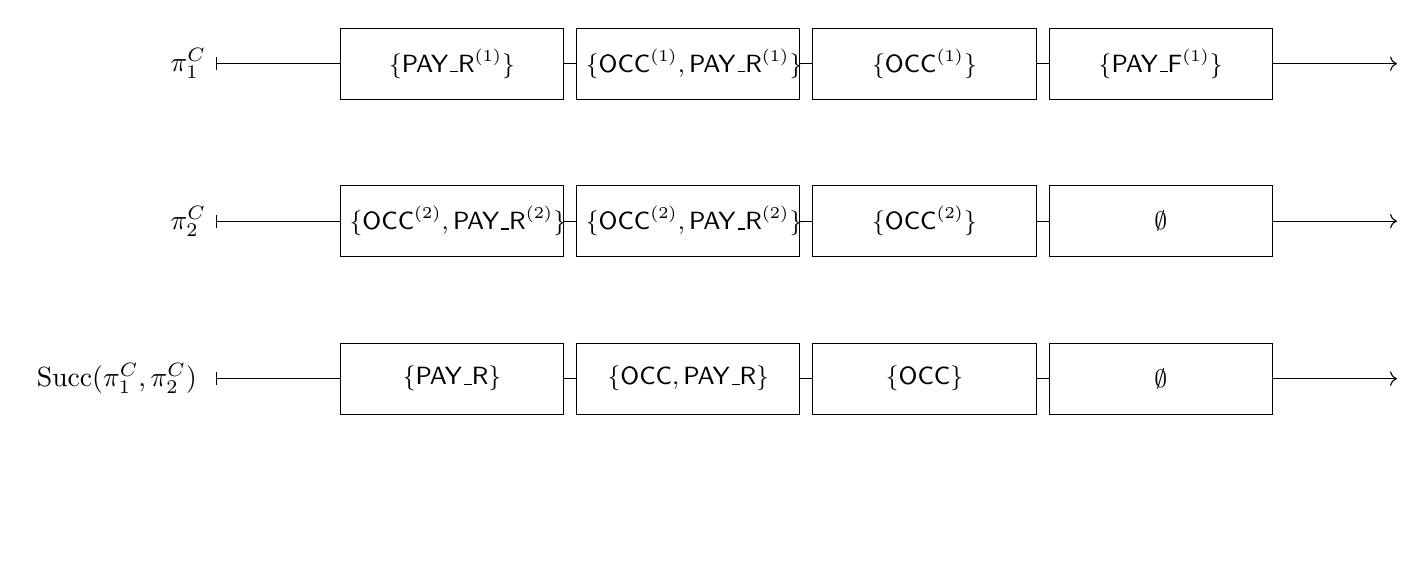
\begin{tikzpicture}[y=2cm,x=3cm]
    % Uniform rectangle nodes for all events (no colors)
    \tikzset{
      event/.style={
        draw,
        rectangle,
        text width=26mm,     % fixed width for all nodes
        minimum height=9mm,  % fixed height for all nodes
        align=center,
        font=\small
      }
    }
  
    % top row: agent 1 (tagged)
    \node[event] at (1,0)   (t1) {$\{\pay{1}\}$};
    \node[event] at (2,0)   (t2) {$\{\occ{1},\pay{1}\}$};
    \node[event] at (3,0)   (t3) {$\{\occ{1}\}$};
    \node[event] at (4,0)   (t4) {$\{\payf{1}\}$};
  
    % middle row: agent 2 (tagged)
    \node[event] at (1,-1)  (l1) {$\{\occ{2},\pay{2}\}$};
    \node[event] at (2,-1)  (l2) {$\{\occ{2},\pay{2}\}$};
    \node[event] at (3,-1)  (l3) {$\{\occ{2}\}$};
    \node[event] at (4,-1)  (l4) {$\emptyset$};
  
    % bottom row: success = unlabel + intersection
    \node[event] at (1,-2) (h1) {$\{\PAY\}$};
    \node[event] at (2,-2) (h2) {$\{\OCC,\PAY\}$};
    \node[event] at (3,-2) (h3) {$\{\OCC\}$};
    \node[event] at (4,-2) (h4) {$\emptyset$};
  
    % time/progression connectors
    \path[shorten >=0pt]
      (0,0) node[left] {$\pi_1^{C}$} edge[|-]
      (t1) (t1) edge (t2) (t2) edge (t3) (t3) edge (t4) (t4) edge[->] +(1,0)
      (0,-1) node[left] {$\pi_2^{C}$} edge[|-]
      (l1) (l1) edge (l2) (l2) edge (l3) (l3) edge (l4) (l4) edge[->] +(1,0)
      (0,-2) node[left, align=center] {$\mathrm{Succ}(\pi_1^{C}, \pi_2^{C})$ } edge[|-]
      (h1) (h1) edge (h2) (h2) edge (h3) (h3) edge (h4) (h4) edge[->] +(1,0)
      (0,-3);
  \end{tikzpicture}}}
  {Example: successful collaboration computation example}
  {example:succ-meet}
  {\vspace{10pt}}{\vspace{-18pt}}
  \end{example}
  
  \noindent\textbf{Basic properties.}
  Since \(\mathrm{Succ}\) is pointwise set intersection after tag erasure,
  it inherits three immediate facts:
  \emph{(i) Commutative and idempotent}:
  \(\mathrm{Succ}(\pi_1,\pi_2)=\mathrm{Succ}(\pi_2,\pi_1)\) and
  \(\mathrm{Succ}(\pi,\pi)=\unlab(\pi)\).
  \emph{(ii) Monotone (pointwise \(\subseteq\))}: writing
  \(\pi\le\pi'\) to mean
  \(\forall k:\ \unlab(\pi[k])\subseteq\unlab(\pi'[k])\),
  if \(\pi_1\le\pi_1'\) and \(\pi_2\le\pi_2'\) then
  \(\mathrm{Succ}(\pi_1,\pi_2)\le \mathrm{Succ}(\pi_1',\pi_2')\).
  \emph{(iii) Absorbing empty trace}:
  if \(\forall k,\ \pi_2[k]=\emptyset\),
  then \(\forall k,\ \mathrm{Succ}(\pi_1,\pi_2)[k]=\emptyset\).
  
  \begin{remark}{Relation to \(\parallel_{\mathrm{hs}}^{A}\).}
  If we declare every collaborative objective to be a handshake,
  \(A=\Sigma_C\), then the lockstep-with-handshakes product enforces that
  \(\PAY\), \(\PAYF\), \(\OCC\) can only appear at a period when both agents
  present the same letter. Concretely, if we view each period’s set
  \(A^{(i)}_k\) as the multiset of letters occurring “at that round” and apply
  \(\parallel_{\mathrm{hs}}^{A}\) round wise, then after collapsing paired
  handshakes to a single shared symbol (via \(\mathsf{coll}_A\)) and unlabeling,
  We obtain exactly the success:
  \[
  \mathrm{Succ}(\pi_1,\pi_2)
  \ =\
  \unlab\!\big(\mathsf{coll}_{\Sigma_C}\big(\pi_1\parallel_{\mathrm{hs}}^{\Sigma_C}\pi_2\big)\big),
  \]
  i.e., \(\mathrm{Succ}\) is the set-theoretic intersection semantics of
  lockstep-plus-handshakes on the collaboration alphabet.    
  \end{remark}
  
  \subsection{Second Contribution: Modeling Agent Interaction Strategies}
  Instead of reconstructing compliance post hoc from past events, the approach models how agents intend to behave in the future. Agents may wish to run their intended strategies against the contract to determine compliance, prevent future violations, and identify how other parties may potentially obstruct or exploit the contract.
  
  Because collaborative success depends on both parties, each agent devises a strategy conditioned on the observed behavior of the other. For example, the landlord may plan differently depending on whether the tenant pays, while the tenant may stop paying if the landlord prevents continued occupancy or fails to repair reported damages.
  
  
  
  \subsubsection{Models for Interaction Strategies}
  
  We capture interaction strategies with \emph{input/output} models that operate at the period granularity.
  At each period $k$, each agent $i$ observes the other agent's period-$k$ output and updates its
  internal state to produce its own period-$(k{+}1)$ output. We use \emph{Moore machines} so that an
  agent’s output at period $k$ depends only on its current state (perfect monitoring with one-period delay).
  A synchronous feedback composition couples the two machines.
  
  % In the preamble (once):
  % \newcommand{\PAY}{\mathsf{PAY}}
  % \newcommand{\PAYF}{\mathsf{PAYF}}
  % \newcommand{\OCC}{\mathsf{OCC}}
  % \newcommand{\unlab}{\mathsf{unlab}}
  
  \begin{definition}[Deterministic Moore machine]
  \label{def:moore}
  A deterministic Moore machine for agent $i$ is a 6-tuple
  \[
  M_i \;=\; (S_i, s^0_i,\ \Sigma_I^i,\ \Sigma_O^i,\ \delta_i,\ \lambda_i),
  \]
  where:
  \begin{itemize}
    \item $S_i$ is a finite set of states with initial state $s^0_i\in S_i$;
    \item $\Sigma_I$ is the input alphabet (the other agent’s \emph{untagged} collaborative letters);
    \item $\Sigma_O^i$ is the set of output alphabet;
    \item $\delta_i: S_i \times 2^{\Sigma_I} \to S_i$ is a deterministic transition function;
    \item $\lambda_i: S_i \to 2^{\Sigma_O}$ is the output function.
  \end{itemize}
  Given an input stream $X=(X_0,X_1,\dots)$ with $X_k\subseteq\Sigma_I$, the induced run is
  $s^0_i,s^1_i,\dots$ with $s^{k+1}_i=\delta_i(s^k_i,X_k)$ and outputs $Y_k=\lambda_i(s^k_i)$.
  \end{definition}
  
  \begin{definition}[Run and output of a deterministic Moore machine]
    \label{def:moore-run}
    Let 
    \[
    M_i \;=\; (S_i, s^0_i,\ \Sigma_I^i,\ \Sigma_O^i,\ \delta_i,\ \lambda_i)
    \]
    be a deterministic Moore machine for agent $i$ as in Definition~\ref{def:moore}.
    An \emph{input stream} for $M_i$ is a finite or infinite sequence 
    $X = (X_0,X_1,\dots)$ with $X_k \subseteq \Sigma_I^i$ for all positions $k$.
    
    \medskip
    \noindent\textbf{Run.}
    The \emph{run of $M_i$ on $X$} is the unique sequence of states
    \[
    \rho_i(X) \;=\; (s^0_i,s^1_i,s^2_i,\dots)
    \]
    inductively defined by
    \[
    s^{0}_i := s^0_i,
    \qquad
    s^{k+1}_i := \delta_i(s^k_i, X_k)
    \quad\text{for all }k \ge 0.
    \]
    
    \noindent For finite input $X$ of length $n{+}1$ we write $|X|=n{+}1$ and 
    $\rho_i(X) = (s^0_i,\dots,s^{n+1}_i)$.
    
    \medskip
    \noindent\textbf{Extended transition function.}
    For later use, we define the extended transition function
    \[
    \delta_i^{*} : S_i \times (2^{\Sigma_I^i})^{*} \to S_i
    \]
    by
    \[
    \delta_i^{*}(s, \varepsilon) := s,
    \qquad
    \delta_i^{*}(s, X_0\cdot X') := 
    \delta_i^{*}\bigl(\delta_i(s,X_0),\,X'\bigr),
    \]
    for $X_0 \in 2^{\Sigma_I^i}$ and $X' \in (2^{\Sigma_I^i})^{*}$.
    For a finite input word $X$, we write
    \[
    \delta_i(s^0_i,X) \;:=\; \delta_i^{*}(s^0_i,X),
    \]
    so that the last state of the run on $X$ is $\delta_i(s^0_i,X)$.
    
    \medskip
    \noindent\textbf{Output word and terminal output.}
    The \emph{output word} induced by $M_i$ on $X$ is
    \[
    \lambda_i^{\omega}(X) \;:=\; (Y_0,Y_1,\dots)
    \quad\text{with}\quad
    Y_k := \lambda_i(s^k_i).
    \]
    For a finite input word $X$ the \emph{terminal output} of $M_i$ on $X$ is
    \[
    \lambda_i\bigl(\delta_i(s^0_i,X)\bigr),
    \]
    which is the output associated with the last state of the run on $X$.
    \end{definition}
  
  \subsubsection{Interactive Strategy Computation}
  
  We present the property of two Moore machines that can feed each other and progress together.
  
  \begin{definition}[Complementary Moore machines]
  \[\text{Let } 
  M_i \;=\; (S_i, s^0_i,\ \Sigma_I^i,\ \Sigma_O^i,\ \delta_i,\ \lambda_i) \text{ and } M_j \;=\; (S_j, s^0_j,\ \Sigma_I^j,\ \Sigma_O^j,\ \delta_j,\ \lambda_j) 
  \]
  be two deterministic Moore machines, we say that \emph{$M_i$ and $M_j$ are complementary} if and only if:
  \[ \Sigma_I^i = \Sigma_O^j \text{ and } \Sigma_O^i = \Sigma_I^j.\]
  \end{definition}
  In the following, we introduce an example of how to use Moore machines to capture two strategies that the landlord and the tenant should consider in the motivating example.
  \begin{example}[Interaction strategies and their Moore encodings]
  \label{ex:twomoore}
  Consider the two first informal strategies $\strat_1^1$ and $\strat_2^1$ from respectively the tenant(1) and the landlord(2):
  
  \medskip
  \noindent\textbf{Tenant $\strat_1^1$.}
  “I pay in the first month; from the second month on, I occupy and keep paying as long as the landlord does not stop me. If the landlord stops my occupancy, I stop paying.”
  
  \noindent\textbf{Landlord $\strat_2^1$.}
  “I enable occupancy from the first month and accept payment; if the tenant fails to pay for \emph{two consecutive} months, I stop enabling occupancy.”
  We encode both of those strategies using: $\Sigma_C^{(1)}:=\{a^{(1)}\mid a\in\Sigma_C\}$ and
  $\Sigma_C^{(2)}:=\{a^{(2)}\mid a\in\Sigma_C\}$ be the tagged disjoint copies.
  Both machines use $S=\{s_0,s_1,s_2\}$ with initial state $s_0$.
  Transitions are guarded by the current letters of the agent \emph{other} (seen as a set).
  
  \begin{figure}[h]
  \centering
  \begin{subfigure}[t]{0.70\textwidth}
  \centering
  \scalebox{0.9}{
  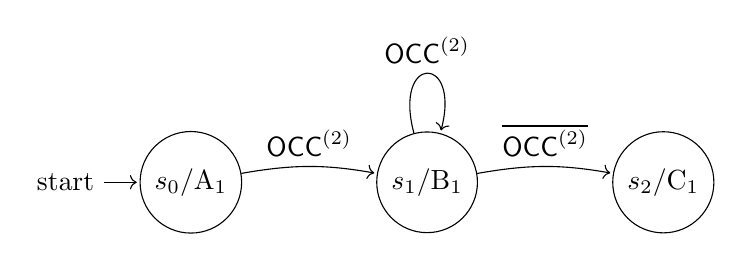
\begin{tikzpicture}[shorten >=1pt,node distance=3cm,on grid,auto]
    % Tenant machine M_1^1
    \node[state,initial] (s_0) {$s_0/\mathrm{A_1}$};
    \node[state,right=of s_0] (s_1) {$s_1/\mathrm{B_1}$};
    \node[state,right=of s_1] (s_2) {$s_2/\mathrm{C_1}$};
  
    \path[->]
      (s_0) edge[bend left=10] node {$\OCC^{(2)}$} (s_1)
      (s_1) edge[loop above] node {$\OCC^{(2)}$} ()
            edge[bend left=10] node {$\overline{\OCC^{(2)}}$} (s_2);
  \end{tikzpicture}}
  \caption{$M_1^1$ (tenant).\\ $\mathrm{A_1}=\{\PAY^{(1)}\}$, $\mathrm{B_1}=\{\OCC^{(1)},\PAY^{(1)}\}$, $\mathrm{C_1}=\emptyset$.}
  \label{fig:moore-tenant}
  \end{subfigure}
  
  \begin{subfigure}[t]{0.70\textwidth}
  \centering
  \scalebox{0.9}{
  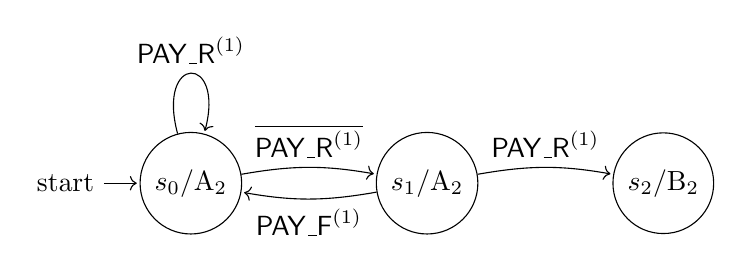
\begin{tikzpicture}[shorten >=1pt,node distance=3cm,on grid,auto]
    % Landlord machine M_2^1
    \node[state,initial] (s_0) {$s_0/\mathrm{A_2}$};
    \node[state,right=of s_0] (s_1) {$s_1/\mathrm{A_2}$};
    \node[state,right=of s_1] (s_2) {$s_2/\mathrm{B_2}$};
  
    \path[->]
      (s_0) edge[loop above] node {$\PAY^{(1)}$} ()
            edge[bend left=10] node {$\overline{\PAY^{(1)}}$} (s_1)
      (s_1) edge[bend left=10] node {$\PAYF^{(1)}$} (s_0)
            edge[bend left=10] node {$\PAY^{(1)}$} (s_2);
  \end{tikzpicture}}
  \caption{$M_2^1$ (landlord). Outputs: $\mathrm{A_2}=\{\OCC^{(2)},\PAY^{(2)}\}$, $\mathrm{B_2}=\emptyset$.}
  \label{fig:moore-landlord}
  \end{subfigure}
  
  \caption{Moore machines for the tenant and landlord representing their strategies over tagged $\Sigma_C$.
  In the transition, the $\lnot \PAY^{i}$ in the Moore machine $M_j$ is a shorthand for any input from $M_i$ not containing $\PAY^{i}$, similarly $\PAY^{i}$ is a shorthand for any input from $M_i$ containing $\PAY^{i}$}
  \label{fig:moore-strategies}
  \end{figure}
  
  \noindent\textit{Formalization (matching Fig.~\ref{fig:moore-strategies}).}
  \[
  \begin{aligned}
  M_1^1&=(S,s_0,\ \Sigma_I^{(1)},\Sigma_O^{(1)},\ \delta_1,\lambda_1),
  &\Sigma_I^{(1)}&=2^{\Sigma_C^{(2)}},& \Sigma_O^{(1)}&=2^{\Sigma_C^{(1)}},\\
  M_2^1&=(S,s_0,\ \Sigma_I^{(2)},\Sigma_O^{(2)},\ \delta_2,\lambda_2),
  &\Sigma_I^{(2)}&=2^{\Sigma_C^{(1)}},& \Sigma_O^{(2)}&=2^{\Sigma_C^{(2)}}.
  \end{aligned}
  \]
  For $X\subseteq\Sigma_C^{(2)}$, $Y\subseteq\Sigma_C^{(1)}$:
  \[
  \delta_1(s_0,X)=\begin{cases}s_1&\OCC^{(2)}\in X\\ s_0&\text{otherwise}\end{cases},\ \ 
  \delta_1(s_1,X)=\begin{cases}s_1&\OCC^{(2)}\in X\\ s_2&\text{otherwise}\end{cases},\ \ 
  \delta_1(s_2,X)=s_2,
  \]
  \[
  \delta_2(s_0,Y)=\begin{cases}s_0&\PAY^{(1)}\in Y\\ s_1&\text{otherwise}\end{cases},\ \ 
  \delta_2(s_1,Y)=\begin{cases}s_0&\PAYF^{(1)}\in Y\\ s_2&\PAY^{(1)}\in Y\\ s_1&\text{otherwise}\end{cases},\ \ 
  \delta_2(s_2,Y)=s_2.
  \]
  
  Notice that two Moore machines are complementary.
  \end{example}
  
  Now we move to the step where both strategies are fixed and transformed to compute their outcome. To do so, we introduce the product of two complementary Moore machines.
  
  
  \begin{definition}[Product of Complementary Determinstic Moore Machines]
  
  \[\text{Let }
  M_i \;=\; (S_i, s^0_i,\ \Sigma_I^j,\ \Sigma_O^i,\ \delta_i,\ \lambda_i)
  \quad\text{and}\quad
  M_j \;=\; (S_j, s^0_j,\ \Sigma_I^i,\ \Sigma_O^j,\ \delta_j,\ \lambda_j)
  \]
  be two deterministic complementary Moore machines.
  The \emph{product} of $M_i$ and $M_j$ is the automaton
  \[
  M_i \otimes M_j \;=\; (\,\Sigma,\ Q,\ q_0,\ \delta,\ F\,)
  \]
  where
  \begin{itemize}
      \item $\Sigma = 2^{\Sigma_O^i \cup \Sigma_O^j}$ is the \emph{joint alphabet},
      \item $Q = S_i \times S_j$ is the \emph{state space},
      \item $q_0 = (s^0_i, s^0_j)$ is the \emph{initial state},
      \item $F = \emptyset$ ,
      \item $\delta \subseteq Q \times \Sigma \times Q$ is the \emph{transition relation}, defined by
      \[
      \big((s_i,s_j),\, A,\, (s'_i,s'_j)\big) \in \delta
      \]
      if and only if
      \[
      A = \lambda_i(s_i) \cup \lambda_j(s_j), 
      \quad s'_i = \delta_i(s_i,\lambda_j(s_j)), 
      \quad s'_j = \delta_j(s_j,\lambda_i(s_i)).
      \]
  \end{itemize}
  The \emph{language} $L(M_i \otimes M_j) \subseteq \Sigma^\omega$ consists of all infinite words
  \[
  \trace{A_0, A_1, A_2 \dots}
  \]
  such that there exists a run
  \[
  (s^0_i, s^0_j) \xrightarrow{A_0} (s_{i,1}, s_{j,1}) \xrightarrow{A_1} (s_{i,2}, s_{j,2}) \xrightarrow{A_2} \dots
  \]
  with $A_k = \lambda_i(s_{i,k}) \cup \lambda_j(s_{j,k})$ for all $k \geq 0$.
  \end{definition}
  
  
  
  \begin{lemma}[Unique run and word of product machines]
  \label{lem:product-word}
  Let
  \[
  M_i = (S_i, s^0_i,\ \Sigma_I^j,\ \Sigma_O^i,\ \delta_i,\ \lambda_i)
  \quad\text{and}\quad
  M_j = (S_j, s^0_j,\ \Sigma_I^i,\ \Sigma_O^j,\ \delta_j,\ \lambda_j)
  \]
  be two complementary deterministic Moore machines.  
  Then their product $M_i \otimes M_j$ admits a \emph{unique run}
  \[
  (s^0_i,s^0_j)\,(s_{i,1},s_{j,1})\,(s_{i,2},s_{j,2})\dots
  \]
  and this run induces a \emph{unique word}
  \[
  \pi \;=\; \trace{A_0,A_1,A_2,\dots} \;\in\; \big(2^{\Sigma_O^i \cup \Sigma_O^j}\big)^\omega,
  \]
  where
  \[
  A_t \;=\; \lambda_i(s_{i,t}) \cup \lambda_j(s_{j,t}), \qquad t \ge 0,
  \]
  and the successor states are determined by
  \[
  s_{i,t+1} = \delta_i(s_{i,t},\,\lambda_j(s_{j,t})),\qquad
  s_{j,t+1} = \delta_j(s_{j,t},\,\lambda_i(s_{i,t})).
  \]
  \end{lemma}
  
  \begin{proof}
  Determinism ensures that for every product state $(s_{i,t},s_{j,t})$ there is exactly one
  successor $(s_{i,t+1},s_{j,t+1})$, determined by the mutual feedback of outputs.
  By induction on $t$, this yields a unique run of the product automaton starting from $(s^0_i,s^0_j)$.
  Collecting the joint outputs at each step produces the word $\pi$, which is therefore unique.
  If the run stabilizes in a sink state with constant outputs, $\pi$ is ultimately periodic
  and may be regarded as finite; otherwise $\pi$ is infinite.
  \end{proof}
  
  \begin{example}[Product automaton sketch for $M_1^1 \times M_2^1$]
  \label{ex:product-automaton}
  We now project the two Moore machines $M_1^1$ (tenant) and $M_2^1$ (landlord) of
  Example~\ref{ex:twomoore} into their synchronous product $M_1^1 \times M_2^1$.
  Each state of the product records the joint output of both agents in that period, denoted by $\{A_1,A_2\}$, with $A_1\in 2^{\Sigma_C^{(1)}}$ and $A_2\in 2^{\Sigma_C^{(2)}}$.
  The initial state corresponds to $(s^0_1,s^0_2)$; subsequent states reflect how both machines
  progress under synchronous feedback. Once a stable pair of states is reached, the product
  loops, generating the same joint output forever.
  
  \begin{figure}[h]
  \centering
  \begin{subfigure}[t]{0.70\textwidth}
  \centering
  \scalebox{0.9}{
  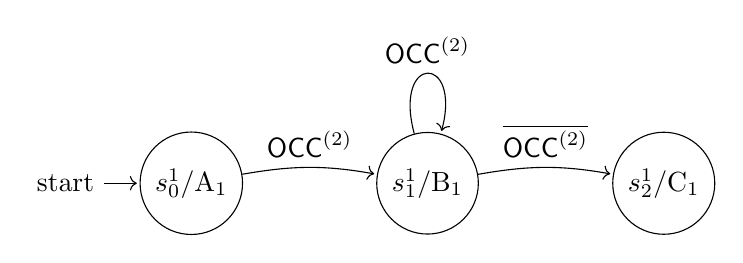
\begin{tikzpicture}[shorten >=1pt,node distance=3cm,on grid,auto]
    % Tenant machine M_1^1
    \node[state,initial] (s_0) {$s_0^1/\mathrm{A_1}$};
    \node[state,right=of s_0] (s_1) {$s_1^1/\mathrm{B_1}$};
    \node[state,right=of s_1] (s_2) {$s_2^1/\mathrm{C_1}$};
  
    \path[->]
      (s_0) edge[bend left=10] node {$\OCC^{(2)}$} (s_1)
      (s_1) edge[loop above] node {$\OCC^{(2)}$} ()
            edge[bend left=10] node {$\overline{\OCC^{(2)}}$} (s_2);
  \end{tikzpicture}}
  \caption{$M_1^1$ (tenant), with\\ $\mathrm{A_1}=\{\PAY^{(1)}\}$, $\mathrm{B_1}=\{\OCC^{(1)},\PAY^{(1)}\}$, $\mathrm{C_1}=\emptyset$.}
  \label{fig:moore-tenant-prod}
  \end{subfigure}
  \vspace{0.5cm}
  \begin{subfigure}[t]{0.70\textwidth}
  \centering
  \scalebox{0.9}{
  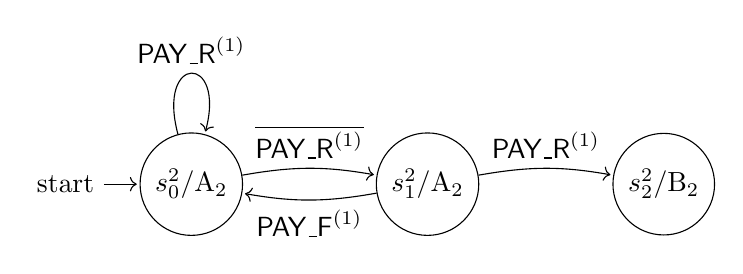
\begin{tikzpicture}[shorten >=1pt,node distance=3cm,on grid,auto]
    % Landlord machine M_2^1
    \node[state,initial] (s_0) {$s_0^2/\mathrm{A_2}$};
    \node[state,right=of s_0] (s_1) {$s_1^2/\mathrm{A_2}$};
    \node[state,right=of s_1] (s_2) {$s_2^2/\mathrm{B_2}$};
  
    \path[->]
      (s_0) edge[loop above] node {$\PAY^{(1)}$} ()
            edge[bend left=10] node {$\overline{\PAY^{(1)}}$} (s_1)
      (s_1) edge[bend left=10] node {$\PAYF^{(1)}$} (s_0)
            edge[bend left=10] node {$\PAY^{(1)}$} (s_2);
  \end{tikzpicture}}
  \caption{$M_2^1$ (landlord), with : $\mathrm{A_2}=\{\OCC^{(2)},\PAY^{(2)}\}$, $\mathrm{B_2}=\emptyset$}
  \label{fig:moore-landlord-prod}
  \end{subfigure}
  \vspace{0.5cm}
  \begin{subfigure}[t]{0.70\textwidth}
  \centering
  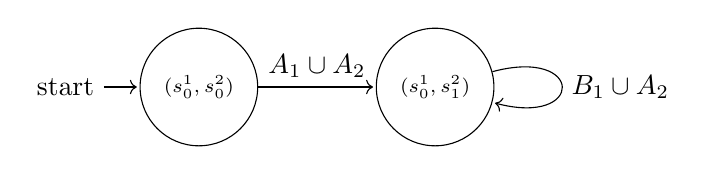
\begin{tikzpicture}[shorten >=1pt,node distance=3cm,on grid,auto,
    every state/.style={inner sep=6pt,font=\scriptsize}]
    % States show pairs of original machine states
    \node[state,initial] (s0) {$(s_0^1,s_0^2)$};
    \node[state, right=of s0] (s1) {$(s_0^1,s_1^2)$};
  
    % Transitions are labeled with the union of outputs
    \path[->]
      (s0) edge node {$A_1 \cup A_2$} (s1)
      (s1) edge[loop right] node {$B_1 \cup A_2$} (s1);
  \end{tikzpicture}
  \caption{Product automaton $M_1^1 \times M_2^1$, with states as pairs $(s_i^1,s_j^2)$ and transitions labeled by the joint outputs.}
  \label{fig:product-sketch}
  \end{subfigure}
  
  \caption{Tenant’s machine $M_1^1$, landlord’s machine $M_2^1$, and their product 
  automaton $M_1^1 \times M_2^1$. 
  Each product state is labeled by the joint output $\lambda_1(s_i^1)\cup\lambda_2(s_j^2)$.}
  \label{fig:moore-product-full}
  \end{figure}
  
  \noindent
  Concretely, The run of the product $M_1^1 \times M_2^1$ in  Fig.~\ref{fig:moore-strategies}, corresponds to the omega-word\\
  $\trace{\{\PAY^{(1)},\OCC^{(2)},\PAY^{(2)}\}~\
   (\{\OCC^{(1)},\PAY^{(1)},\OCC^{(2)},\PAY^{(2)}\})^\omega}.$
  \end{example}
  
  
  
  \section{The Two-Agents Collaborative Normative Logic \cDL}
  \subsection{Syntax of \cDL}
  As summarized in Fig.~\ref{fig:cdl-syntax}, the syntax of \cDL\ is organized into three blocks: regular expressions, literals, and contracts.
  
  \begin{figure}[h]
  \centering
  \fbox{%
  \begin{minipage}{0.96\textwidth}
  \captionof{figure}{Syntax of \cDL}
  \label{fig:cdl-syntax}
  \small
  Given a collaboration alphabet $\Sigma_C$ and let
  $\Sigma := \Sigma_C^{(1)} \cup \Sigma_C^{(2)}$ be the tagged action alphabet.
  With:
  $a \in \Sigma_C$ (collaboration action),\;
  $p \in \{1,2\}$ (party).\;
  $A \in 2^\Sigma$ (party tagged action set),\;
  $n \in \mathbb{N^*}$ (non-zero natural number).\;
  The syntax of \cdl is defined inductively via the following grammar:
  
  \medskip
  \[
  \begin{alignedat}{3}
  \textbf{Regular expressions}\quad
  \re\ &::=&\ \mathsf{A}                                      && \hfill[\text{tagged action set}] \\
     &\mid&\ \Gamma                             && \hfill[\text{trump card}] \\
     &\mid&\ \varepsilon                             && \hfill[\text{empty word}] \\
     &\mid&\ \emptyset                              &&  \hfill\quad\qquad [\text{empty set of actions}] \\
     &\mid&\ (\re \mid \re)                           && \hfill[\text{union}] \\
     &\mid&\ \re \cdot \re                           && \hfill[\text{concatenation}] \\
     &\mid&\ \re^{n}                                  && \hfill[\text{n-repetition}] \\
     &\mid&\ \re^{+}                                  && \hfill[\text{Kleene plus}] \\[6pt]
  %
  \textbf{Literals}\quad
  \ell\ &::=&\ \obl[p]{a}                           && \hfill[\text{obligation}] \\
       &\mid&\ \frb[p]{a}                           && \hfill[\text{prohibition}] \\
       &\mid&\ \perm[p]{a}                          && \hfill[\text{permission}] \\
       &\mid&\ \top                                 && \hfill[\text{valid}] \\
       &\mid&\ \bot                                 && \hfill[\text{invalid}] \\[6pt]
  %
  \textbf{Contracts}\quad
  C\ &::=&\ \ell                                    && \hfill[\text{literal}] \\
    &\mid&\ C \wedge C                              && \hfill[\text{conjunction}] \\
    &\mid&\ C ; C                                   && \hfill[\text{sequence}] \\
    &\mid&\ C \repair C                             && \hfill[\text{reparation}] \\
    &\mid&\ \trig[re]{C}                   && \hfill[\text{triggered}] \\
    &\mid&\ \guard[re]{C}                           && \hfill[\text{guarded}] \\
    &\mid&\ C^n                                     && \hfill[\text{n-repetition}]\\
    &\mid&\ \repit{C}                               && \hfill[\text{infinite-repetition}]
  \end{alignedat}
  \]
  \end{minipage}}
  \end{figure}
  
  
   
  \medskip
  \noindent\textbf{Regular expressions (\emph{re}).}
  This block specifies \emph{when} clauses apply by describing patterns over monthly positions.
  An \emph{atom} is a tagged action-set \(A \subseteq \Sigma\) stating what the two parties did in a month.
  Complex expressions are formed with \emph{union} \((re \mid re)\), \emph{concatenation} \((re \cdot re)\) for next-month sequencing,
  \emph{power} \(re^n\) (exactly \(n\) repetitions), and \emph{Kleene plus} \(re^+\) (one or more repetitions).
  The \emph{wildcard} \(\Gamma\) is the union of all $A \subseteq \Sigma$ used to skip a position, and \(\emptyset\) denotes the \emph{empty set of actions}.
  These constructs enable patterns such as “a repair is requested this month” (an atom), “after any number of months if Agent $1$ asks for termination (\(\Gamma \cdot\)), or “three consecutive months” \((re)^3\).
  
  \medskip
  \noindent\textbf{Literals (\emph{\(\ell\)}).}
  This block provides the primitive deontic statements for a single month:
  \emph{obligation} \(\obl[p]{a}\), \emph{prohibition} \(\frb[p]{a}\), and \emph{power} \(\perm[p]{a}\),
  plus the constants \emph{valid} \(\top\) and \emph{invalid} \(\bot\).
  Here \(p \in \{1,2\}\) identifies the party (tenant or landlord) and \(a \in \Sigma_C\) is a collaboration action.
  Intuitively, literals say \emph{what} is required/forbidden/allowed of \emph{whom}, independently of timing.
  
  \medskip
  \noindent\textbf{Contracts (\emph{C}).}
  This block composes literals into full specifications using:
  \emph{conjunction} \((C \wedge C)\) to combine requirements in the same time position;
  \emph{sequence} \((C;C)\) for next-time progression;
  \emph{reparation} \((C \repair C')\) for contrary-to-duty fall-backs saying you are requested to perform $C$, if you fail you must conform to $C'$ in the next time position;
  \emph{triggered} clauses \(\trig[re]{C}\) that activate \(C\) when a pattern \(re\) occurs;
  \emph{guarded} clauses \(\guard[re]{C}\) that encapsulate conditions under which conforming to a contract is no longer necessary; and
  \emph{repetition} \(\repit{C}\) for repetitive occurrence of a contract.
  Together, these constructs could be used to capture the clauses of a contract, the conditions under which they are activated or terminated, and how the clauses relate to each other regarding reparations or the timing of their application. More specifically, the combination of repetition and a guarded contract can capture the notion of open-ended contracts.
   In the following example, we illustrate how we could capture our motivating example:
  \subsection{Illustrating the Encoding in \cDL for the Motivating Example}
  \begin{example}[Encoding the rental clauses in \cDL]
  \label{ex:contract-encoding}
  We now illustrate how the rental agreement introduced in Example~\ref{ME} 
  can be systematically encoded in the \cDL\ syntax (see Fig.~\ref{fig:cdl-syntax}).  
  We define the collaboration alphabet that captures all joint actions relevant to the contract:
  \[
  \Sigma_C = \{\PAY,\ \PAYF,\ \OCC,\ \notifrepair,\ \notifterm,\ \REPAIR\}.
  \]
  Each element corresponds to a collaborative outcome:
  \PAY\ (rent payment), \PAYF\ (late fee payment), \OCC\ (occupancy), 
  \notifrepair\ (tenant’s repair request), \notifterm\ (termination notice), 
  and \REPAIR\ (landlord performing repair).
  
  \medskip
  The encoding proceeds clause by clause, following the contract structure:
  
  \begin{itemize}
    \item \textbf{C1 (Tenant pays rent):}  
    The tenant is obliged to pay the rent each month.  
    \[
    C_1 := \obl[1]{\PAY}.
    \]
  
    \item \textbf{C2 (Landlord guarantees occupancy):}  
    The tenant gets the power to occupy the flat. 
    Thus, the landlord is required not to interfere with the tenant’s occupancy, 
    encoded as a permission to allow the collaborative outcome \OCC.  
    \[
    C_2 := \perm[1]{\OCC}.
    \]
  
    \item \textbf{C3 (Late-payment reparation):}  
    Clause C3 introduces a contrary-to-duty (CTD) structure: if the tenant fails to fulfill the primary obligation (C1), a compensatory obligation to pay the late fee arises.  
    This relationship is encoded as a reparation construct:
    \[
    C_3 := \obl[1]{\PAY}\ \repair\ \obl[1]{\PAYF}.
    \]
  
    \item \textbf{C4 (Triggered repair request):}  
    The tenant’s request for repairs activates the landlord’s duty to perform them within the following month.  
    This is expressed using a triggered clause:
    \[
    C_4 := 
    \trig[\{\notifrepair^{(1)}\}]{\obl[2]{\REPAIR}}.
    \]
  
    \item \textbf{C5 (Termination and continuation):}  
    The tenant may terminate the contract unilaterally by issuing a termination notice.  
    After this notice, the contract’s active obligations (rent, occupancy, repairs) 
    persist for three additional months before ending.  
    This behavior is captured with a guarded contract:
    \[
    C_5 := \guard[\,\Gamma^+ \cdot \{\notifterm^{(1)}\} \cdot \Gamma^{3}\,] (\ C_3\ \wedge\ C_2\ \wedge\ C_4\ ).
    \]
  \end{itemize}
  
  \medskip
  This step-by-step encoding shows how \cDL\ integrates temporal regular patterns, deontic modalities, 
  and event-triggered obligations in a single formalism.  
  Clauses (C1–C5) together specify a full-cycle contract where collaborative actions such as payment, occupancy, repair, and termination are modeled as 
  conditional and time-bounded obligations between the two agents.
  \end{example}
  
  
  We move now to the first semantic definition for this logic, where we just care about whether a contract was satisfied.



\section{The Notion of Tight Semantics}
\label{sec:motivate-tight}


In \cdl, contracts integrate responsibilities across multiple agents and temporal dimensions, making timing integral to their interpretation. Each duty is associated with a specific moment, and failure to fulfill it punctually results in an immediate contractual shift: the violation is registered at a distinct point, after which reparation obligations are activated. Semantically, this necessitates partitioning a trace into a \emph{pre-violation} prefix and a \emph{post-violation} suffix, with the reparation component evaluated exclusively on the post-violation segment.

This partitioning must be exact. It is necessary to identify a unique earliest violation point, and correspondingly, a unique earliest satisfaction point, to ensure a single, unambiguous decomposition of observed behavior into segments occurring before and after the decisive instant. In the absence of such a unique boundary, reparations may be initiated prematurely, belatedly, or multiple times, leading to ambiguity in responsibility attribution. The prefix-based tight semantics introduced below are constructed to isolate these unique boundaries and thereby render the before-and-after evaluation well-defined.

This approach is termed \emph{tight forward} semantics. The term \emph{forward} indicates that each verdict is determined sequentially from left to right over prefixes, without reference to future events, and that contract progression follows the chronological order of the trace. The term \emph{tight} signifies that the semantics are anchored at the first decisive instant, isolating a unique earliest satisfaction frontier and a unique earliest violation frontier, and classifying all strict extensions as post-frontier, thus precluding repeated triggering of the same responsibility. Thus, \emph{tight forward} denotes a prefix-based, left-to-right evaluation with a uniquely defined division between pre- and post-frontier phases.

\medskip
\noindent
\textbf{What goes wrong without tightness.}
If we only tag a prefix as ``accepted'' whenever it spells a word in the target
language and keep tagging all longer extensions as ``accepted'' again, we
\emph{lose} the unique earliest acceptance point.  This leads to
(i) ambiguity about \emph{when} credit is earned,
(ii) potential ``double counting'' of compliance,
and (iii) difficulty aligning guarded/triggered clauses with the moment they
should switch on or off.  Dually, labeling every failing extension as a fresh
violation blurs \emph{when} the duty was first broken.

\medskip
\noindent
\textbf{Tiny illustration.}
Let \(\Sigma=\{a,b\}\) and \(L=\{a\}\) (``seeing \(a\) once is success'').
Reading \(a\) at the first position should \emph{decide} compliance then and
there; the longer words \(aa,ab,\dots\) must be treated as \emph{after} the
decision, not as new acceptances.  Conversely, reading \(b\) first fixes the
earliest failure; \(ba,bb,\dots\) are merely \emph{after} that failure.

\medskip
\noindent
\textbf{What tight semantics will guarantee.}
Our five-valued, prefix-oriented view will:
\begin{itemize}
  \item identify the \emph{first acceptance} index (earliest satisfaction);
  \item identify the \emph{first rejection} index (earliest violation);
  \item classify any strict extension \emph{after} these frontiers as ``post'' acceptance/rejection;
  \item mark all prefixes that are still undecided but extendable to acceptance as \emph{pre-eager}.
\end{itemize}
This yields determinacy (exactly one verdict per prefix), uniqueness of frontiers,
and monotone \emph{evolution} of verdicts along extensions—properties crucial for
correctness, fairness, and auditable timing in contracts.

\medskip
\noindent
Building on this motivation, the following section introduces the language-theoretic operators and automata constructions that establish these frontiers and subsequently define
the tight five-valued semantics.

\subsection{From Language Membership to Tight Prefix}
\label{sec:lang-frontiers-tight}

In this subsection, we generalize the construction of tight semantics to \emph{any regular language} $L \subseteq \Sigma^*$.
To do so, we must distinguish between the classical notion of \emph{static language membership} and the requirements of \emph{behaviour evaluation}.

Standard language theory evaluates a word $w$ holistically: $w$ is either inside or outside $L$.
From the normative, behaviour-oriented point of view, we instead ask whether the desired behaviour has \emph{already} been achieved on some prefix.
This requires a prefix-sensitive notion of evaluation together with \emph{eagerness}: we must identify the \emph{first} prefix at which the behaviour becomes satisfied or becomes impossible.
This viewpoint diverges from plain set membership.
For example, if $L=\{a\}$, the word $aa$ is not in $L$ (it is rejected by language membership).
However, for behavioural monitoring, the prefix $a$ already establishes success; the second $a$ is merely an irrelevant extension, not a failure.

Our objective is to formalize this shift by partitioning $\Sigma^*$ into regions that isolate these \emph{boundaries of decision}, explicitly resolving conflicts between ``bad words'' and ``extensions of good words'' in favor of the latter.

\subsubsection{Topological Boundaries}
We begin by identifying the candidate boundaries using standard topological operators on strings: the viable prefixes and the minimal evidence for membership or exclusion.

\begin{definition}[Closures and Frontiers]\label{def:closure-bad}
    For a regular language $L \subseteq \Sigma^*$:
    \begin{enumerate}
        \item The \textbf{Prefix Closure} ($\closureclass{L}$) is the set of all prefixes of words in $L$.
        \item The \textbf{Bad Class} ($\badclass{L}$) is the complement of the closure (prefixes that can never lead to acceptance).
        \item The \textbf{Minimal Frontier} ($\minlang{S}$) of a set is the set of its shortest elements.
    \end{enumerate}
\end{definition}

Applying the minimal frontier operator yields two sets of candidates:
\begin{itemize}
    \item $\minlang{L}$: The candidates for \emph{Eager Acceptance} (shortest words in $L$).
    \item $\minlang{\badclass{L}}$: The candidates for \emph{Eager Rejection} (shortest words deviating from $L$).
\end{itemize}

\subsubsection{The Priority of Acceptance}
A rigorous definition of monitoring behavior requires resolving semantic overlaps between these frontiers.
A word can be a minimal bad prefix while simultaneously extending a minimal accepted word (e.g., as noted, $aa$ regarding $L=\{a\}$).

To ensure deterministic, forward-looking behavior, we enforce a \textbf{priority of acceptance}:
Once a trace reaches the acceptance frontier $\minlang{L}$, any further extension is classified as \emph{irrelevant post-acceptance}, regardless of whether that extension technically belongs to $\badclass{L}$.

\begin{definition}[Canonical Semantic Partition]\label{def:partition-sets}
    We define the five disjoint sets forming the partition of $\Sigma^*$ as follows:
    \begin{align*}
        \EAL{L} &:= \minlang{L}                                  && \text{(Eager Acceptance)} \\
        \IAL{L} &:= \EAL{L}\,\Sigma^{+}                          && \text{(Irrelevant Acceptance)} \\
        \ERL{L} &:= \minlang{\badclass{L}} \setminus \IAL{L}     && \text{(Eager Rejection)} \\
        \IRL{L} &:= \ERL{L}\,\Sigma^{+}                          && \text{(Irrelevant Rejection)} \\
        \Pre{L} &:= \closureclass{\EAL{L}} \setminus \EAL{L}     && \text{(Pre-Verdict / Unknown)}
    \end{align*}
\end{definition}

\noindent
The critical operation here is the subtraction in $\ERL{L}$.
By removing $\IAL{L}$ from the bad frontier, we formally encode the shift from membership to monitoring: determining that a trace is ``bad'' is meaningful only if it has not already been declared ``good.''

\paragraph{Deconstructing regular language for tight behavior}
\paragraph*{Disjoint and complementary notation.}
We write $X = A \dotcup B$ to mean that $A$ and $B$ are disjoint and $X=A\cup B$.

Using this notation our goal is to decompose any regular language into disjoint and complementary sub-language related to behavioral acceptance/rejection.
\begin{lemma}\label{lem:basic}
For any $L\subseteq\Sigma^*$:
\begin{enumerate}
  \item $\minlang{L}\ \subseteq\ \closureclass{L}$,\quad
        $\minlang{\badclass{L}}\ \subseteq\ \badclass{L}$,\quad
        and\quad $\minlang{L}\ \cap\ \minlang{\badclass{L}}=\emptyset$.
  \item $\closureclass{\minlang{L}}=\bigl\{\,u\mid \exists m\in\minlang{L}:\ u\preceq m\,\bigr\}
        \ =\ \bigl(\closureclass{\minlang{L}} \setminus \minlang{L}\bigr)\ \dotcup\ \minlang{L}$.
\end{enumerate}
\end{lemma}

\begin{proof}
(1) The inclusion $\minlang{L}\subseteq \closureclass{L}$ is immediate since every
$m\in\minlang{L}$ is itself a prefix of a word in $L$ (namely $m$). Likewise
$\minlang{\badclass{L}}\subseteq \badclass{L}$ holds by definition of minimality
within $\badclass{L}$. Disjointness follows because
$\closureclass{L}\cap \badclass{L}=\emptyset$.

(2) By definition of prefix-closure over the set of minimal acceptances.
The decomposition into the disjoint union with $\minlang{L}$ is immediate since
$\minlang{L}\subseteq \closureclass{\minlang{L}}$ and the difference removes exactly the minimal elements.
\end{proof}




\begin{lemma}[Two canonical splits]\label{lem:two-splits}
For any $L\subseteq\Sigma^*$,
\[
\closureclass{L} \ =\ \closureclass{\minlang{L}}\ \dot\cup\ \IAL{L},
\qquad
\badclass{L} \ =\ \ERL{L}\ \dot\cup\ \IRL{L}.
\]
\end{lemma}

\begin{proof}[Proof sketch]
For $u\in\closureclass{L}$ pick $z\in L$ with $u\preceq z$ and let $m$ be a shortest accepted prefix
of $z$; then $m\in\minlang{L}$. Either $u\preceq m$ (so $u\in\closureclass{\minlang{L}}$) or $m\prec u$
(so $u\in m\Sigma^{+}\subseteq \IAL{L}$).
For the bad side, every $u\in\badclass{L}$ has a unique shortest bad prefix $b\in\minlang{\badclass{L}}$ with $b\preceq u$;
if $b\notin \IAL{L}$ then either $u=b\in\ERL{L}$ or $u\in b\Sigma^{+}\subseteq \IRL{L}$; if $b\in\IAL{L}$ it is assigned to acceptance-overshoot by convention.
\end{proof}

\begin{lemma}[Cross disjointness]\label{lem:cross}
For any $L\subseteq\Sigma^*$,
\[
\closureclass{L}\cap \badclass{L}=\emptyset,\qquad
\IRL{L}\cap \IAL{L}=\emptyset,\qquad
\minlang{L}\cap \IRL{L}=\emptyset.
\]
\end{lemma}


  \begin{proof}
    The first claim follows directly from the definition, as $\badclass{L}$ is the set-theoretic complement of $\closureclass{L}$ in $\Sigma^*$.
    
    For the second claim ($\IRL{L}\cap \IAL{L}=\emptyset$), assume for the sake of contradiction that there exists a word $u \in \IRL{L} \cap \IAL{L}$.
    By the definitions of irrelevant rejection and acceptance, we have $u = b\concat x$ for some $b \in \ERL{L}, x \in \Sigma^+$ and $u = m\concat y$ for some $m \in \EAL{L}, y \in \Sigma^+$.
    Since both $b$ and $m$ are prefixes of $u$, they are comparable.
    If $m \preceq b$, then $b$ extends a minimal accepted word, implying $b \in \IAL{L}$, which contradicts $b \in \ERL{L}$ (since $\ERL{L}$ is defined as $\minlang{\badclass{L}} \setminus \IAL{L}$).
    Conversely, if $b \preceq m$, then the accepted word $m$ extends a bad prefix $b$. However, since $b \in \badclass{L}$, no extension of $b$ can ever belong to $L$, contradicting $m \in L$. Thus, the intersection must be empty.
    
    For the third claim ($\minlang{L} \cap \IRL{L} = \emptyset$), we rely on the fundamental distinction between accepted and bad traces.
    By definition, $\minlang{L}$ contains only words that belong to $L$ (specifically, the shortest ones).
    In contrast, $\IRL{L}$ is a subset of $\badclass{L}$ (extensions of minimal bad prefixes), which contains only words that are strictly outside $\closureclass{L}$.
    Since a word cannot be simultaneously accepted (in $L$) and a bad prefix (in $\badclass{L}$), the sets are disjoint.
    \end{proof}




\paragraph{Five semantic regions.}
We now make the outcome of the previous constructions explicit by introducing a canonical partition of $\Sigma^*$ into five semantic regions. Each region corresponds to a distinct monitoring status of a prefix: before any decision, at the exact point of decision, or strictly after that point. This partition is the semantic backbone of tight prefix evaluation.

\begin{definition}[Five semantic regions]\label{def:five-regions}
For any $L\subseteq\Sigma^*$, define:
\[
\underbrace{\closureclass{\minlang{L}}\setminus \minlang{L}}_{\text{\emph{pre-eager-verdict}}}
\ \dot\cup\
\underbrace{\minlang{L}}_{\text{\emph{eager acceptance}}}
\ \dot\cup\
\underbrace{\ERL{L}}_{\text{\emph{eager rejection}}}
\ \dot\cup\
\underbrace{\IAL{L}}_{\text{\emph{irrelevant acceptance}}}
\ \dot\cup\
\underbrace{\IRL{L}}_{\text{\emph{irrelevant rejection}}}.
\]
\end{definition}



\begin{theorem}[Five-way partition of $\Sigma^*$]\label{thm:five-way}
For every $L\subseteq\Sigma^*$, the space of all possible words could be decomposed into:
\[
\Sigma^{*}
=\ \bigl(\closureclass{\minlang{L}}\setminus \minlang{L}\bigr)
\ \dot\cup\ \minlang{L}
\ \dot\cup\ \ERL{L}
\ \dot\cup\ \IAL{L}
\ \dot\cup\ \IRL{L}.
\]
\end{theorem}

\begin{proof}
From $\Sigma^*=\closureclass{L}\ \dot\cup\ \badclass{L}$ and Lemma~\ref{lem:two-splits},
\[
\Sigma^*=\underbrace{\closureclass{\minlang{L}}\ \dot\cup\ \IAL{L}}_{\closureclass{L}}
\ \dot\cup\
\underbrace{\ERL{L}\ \dot\cup\ \IRL{L}}_{\badclass{L}}.
\]
Now split $\closureclass{\minlang{L}}$ using Lemma~\ref{lem:basic}(2).
Cross disjointness follows from Lemma~\ref{lem:cross}.
\end{proof}


%example
\begin{example}[Five-region decomposition for a simple language]
  Let $\Sigma=\{a,b\}$ and consider the language $L=\{a\}$, meaning that observing
  the symbol $a$ once is sufficient for acceptance.
  
  We first compute the basic classes:
  \begin{align*}
  \closureclass{L} &= \{\varepsilon, a\},\\
  \badclass{L} &= \Sigma^* \setminus \{\varepsilon,a\}
                = \{b, aa, ab, ba, bb, \dots\},\\
  \minlang{L} &= \{a\},\\
  \minlang{\badclass{L}} &= \{b, aa\}.
  \end{align*}
  
  Note that $aa$ is a minimal bad prefix in the language-theoretic sense, yet it
  extends the accepting word $a$. By the priority of acceptance, such extensions
  are classified as post-acceptance rather than as violations.
  
  
  This yields the canonical five-region partition of $\Sigma^*$ by $\Sigma+$ saturation:
 \[
\begin{array}{rcll}
\Pre{L} &:=& \closureclass{\minlang{L}}\setminus \minlang{L}
        \;=\; \{\varepsilon\},
        & \text{(pre-eager verdict)},\\[2pt]
\EAL{L} &:=& \minlang{L}
        \;=\; \{a\},
        & \text{(eager acceptance)},\\[2pt]
\IAL{L} &:=& \EAL{L}\,\Sigma^{+}
        \;=\; a\Sigma^{+},
        & \text{(irrelevant acceptance)},\\[2pt]
\ERL{L} &:=& \minlang{\badclass{L}} \setminus \IAL{L}
        \;=\; \{b\},
        & \text{(eager rejection)},\\[2pt]
\IRL{L} &:=& \ERL{L}\,\Sigma^{+}
        \;=\; b\Sigma^{+},
        & \text{(irrelevant rejection)}.
\end{array}
\]
  
  This example illustrates how tight semantics resolves overlaps between minimal
  acceptance and minimal rejection by assigning all extensions of an accepting
  prefix to the acceptance side, ensuring a unique and deterministic decision
  point.
  \end{example}



\subsubsection{Tight Five-Valued Semantics}
We now introduce a prefix-level semantics that takes values in the set $\tightverdicts=\{\mathsf{?},\topt,\bott,\topp,\botp\}$, corresponding respectively to:
pre-eager verdict (undecided but extendable), eager acceptance (first satisfaction),
eager rejection (first violation), irrelevant acceptance (post acceptance),
and irrelevant rejection (post-rejection).

% \paragraph*{Shortcut notation.}
% For a regular language $L\subseteq\Sigma^*$. For brevity, we fix:
% \[
% \begin{array}{rcll}
% \Pre{L} &:=& \closureclass{\minlang{L}}\setminus \minlang{L}, & \text{(pre-eager verdict)},\\[2pt]
% \EAL{L} &:=& \minlang{L},                                     & \text{(eager acceptance)},\\[2pt]
% \IAL{L} &:=& \EAL{L}\,\Sigma^{+},                         & \text{(irrelevant acceptance)},\\[2pt]
% \ERL{L} &:=& \minlang{\badclass{L}} \ \setminus\ \IAL{L},                                      & \text{(eager rejection)},\\[2pt]
% \IRL{L} &:=& \ERL{L}\,\Sigma^{+}.                            & \text{(irrelevant rejection)}.
% \end{array}
% \]

\begin{definition}[Five-valued prefix semantics]\label{def:five-valued-semantics}
Fix a regular language $L\subseteq\Sigma^*$. For any $u\in\Sigma^*$ define
\[
\semfive{u \vDash L}
\;:=\;
\begin{cases}
\mathsf{?}      & \text{if } u\in \Pre{L},\\[2pt]
\topt            & \text{if } u\in \EAL{L},\\[2pt]
\bott            & \text{if } u\in \ERL{L},\\[2pt]
\topp        & \text{if } u\in \IAL{L},\\[2pt]
\botp      & \text{if } u\in \IRL{L}.
\end{cases}
\]
\end{definition}

\paragraph*{Determinacy.}
By Theorem~\ref{thm:five-way}, the sets $\Pre{L}$, $\EAL{L}$, $\ERL{L}$, $\IAL{L}$, $\IRL{L}$
form a pairwise-disjoint and complete partition of $\Sigma^*$. Hence
$\semfive{u \vDash L}$ is well-defined and single-valued for every $u\in\Sigma^*$.

\begin{theorem}[Prefix Monotonicity and Determinacy]\label{prop:tightness-obligations-unindexed}
  The semantics satisfy the following stability properties for any $u \in \Sigma^*$:
  \begin{enumerate}
      \item \textbf{Monotone evolution along extensions:}
      If $\semfive{u \vDash L}=\topt$ and $x\in\Sigma^{+}$, then
      $\semfive{u\concat x \vDash L}=\topp$.
      If $\semfive{u \vDash L}=\topp$, then for all $x\in\Sigma^{+}$,
      $\semfive{u\concat x \vDash L}=\topp$.
      The dual statements hold for $\bott$ and $\botp$.

      \item \textbf{Unique decision frontier:}
      If $\semfive{u \vDash L}=\topp$, then there exists a unique strict prefix
      $u'\prec u$ such that $\semfive{u' \vDash L}=\topt$.
      Analogously, if $\semfive{u \vDash L}=\botp$, there exists a unique strict prefix
      $u'\prec u$ such that $\semfive{u' \vDash L}=\bott$.

      \item \textbf{Determinism:} Since the partition in Theorem \ref{thm:five-way} is disjoint and complete, the semantics yields exactly one verdict for any input trace.
  \end{enumerate}
\end{theorem}

\begin{proof}
We use only the defining identities from Definition~\ref{def:partition-sets}:
$\EAL{L}:=\minlang{L}$, $\IAL{L}:=\EAL{L}\,\Sigma^{+}$,
$\ERL{L}:=\minlang{\badclass{L}}\setminus\IAL{L}$, and $\IRL{L}:=\ERL{L}\,\Sigma^{+}$.

\smallskip
\noindent\textbf{(1) Monotone evolution along extensions.}
Assume $\semfive{u \vDash L}\in\{\topt,\topp\}$.

If $\semfive{u \vDash L}=\topt$, then $u\in\EAL{L}=\minlang{L}$. For any $x\in\Sigma^{+}$, $u\concat x$ is a strict extension of $u$, so $u\concat x\in \EAL{L}\,\Sigma^{+}=\IAL{L}$ and therefore $\semfive{u\concat x \vDash L}=\topp$.

If $\semfive{u \vDash L}=\topp$, then $u\in\IAL{L}=\EAL{L}\,\Sigma^{+}$. For any $x\in\Sigma^{+}$, $u\concat x$ is a strict extension of $u$, so $u\concat x\in\IAL{L}\,\Sigma^{+}=\IAL{L}$, and again $\semfive{u\concat x \vDash L}=\topp$.

The rejection case is analogous: if $\semfive{u \vDash L}=\bott$ then $u\in\ERL{L}$ and every $u\concat x$ with $x\in\Sigma^{+}$ lies in $\IRL{L}=\ERL{L}\,\Sigma^{+}$, while if $\semfive{u \vDash L}=\botp$ then $u\in\IRL{L}$ and $\IRL{L}$ is closed under strict extensions by definition.

\smallskip
\noindent\textbf{(2) Unique decision frontier.}
Assume $\semfive{u \vDash L}=\topp$. Then $u\in\IAL{L}=\EAL{L}\,\Sigma^{+}$, so there exist $m\in\EAL{L}$ and $x\in\Sigma^{+}$ such that $u=m\concat x$. Let $u':=m$. Then $u'\prec u$ and $\semfive{u' \vDash L}=\topt$.

For uniqueness, suppose $u= m_1\concat x_1 = m_2\concat x_2$ with $m_1,m_2\in\EAL{L}$ and $x_1,x_2\in\Sigma^{+}$. Then both $m_1$ and $m_2$ are prefixes of $u$, hence they are comparable under the prefix order. If $m_1\prec m_2$, then $m_2$ is a strict extension of $m_1$ and cannot belong to $\minlang{L}=\EAL{L}$, contradicting minimality. Symmetrically, $m_2\prec m_1$ is impossible. Therefore $m_1=m_2$, and the strict prefix $u'$ with verdict $\topt$ is unique.

The same reasoning applies to the rejection side: if $\semfive{u \vDash L}=\botp$ then $u\in\IRL{L}=\ERL{L}\,\Sigma^{+}$, so there exist $b\in\ERL{L}$ and $x\in\Sigma^{+}$ such that $u=b\concat x$, and the unique strict prefix with verdict $\bott$ is the unique such $b$ from $\ERL{L}$.

\smallskip
\noindent\textbf{(3) Determinism.}
By Theorem~\ref{thm:five-way}, the sets $\Pre{L}$, $\EAL{L}$, $\ERL{L}$, $\IAL{L}$, and $\IRL{L}$ form a pairwise-disjoint and complete partition of $\Sigma^{*}$. Hence every $u\in\Sigma^{*}$ belongs to exactly one region, so $\semfive{u \vDash L}$ returns exactly one verdict.
\end{proof}

\paragraph{Graphical overview.}
Figure~\ref{prop:tightness-obligations-unindexed} visualizes the five semantic regions and their intended temporal evolution. The layout reflects how a language moves from an undecided language to a decisive frontier and then irreversibly into a post-verdict phase.
\begin{figure}[h]
  \centering
  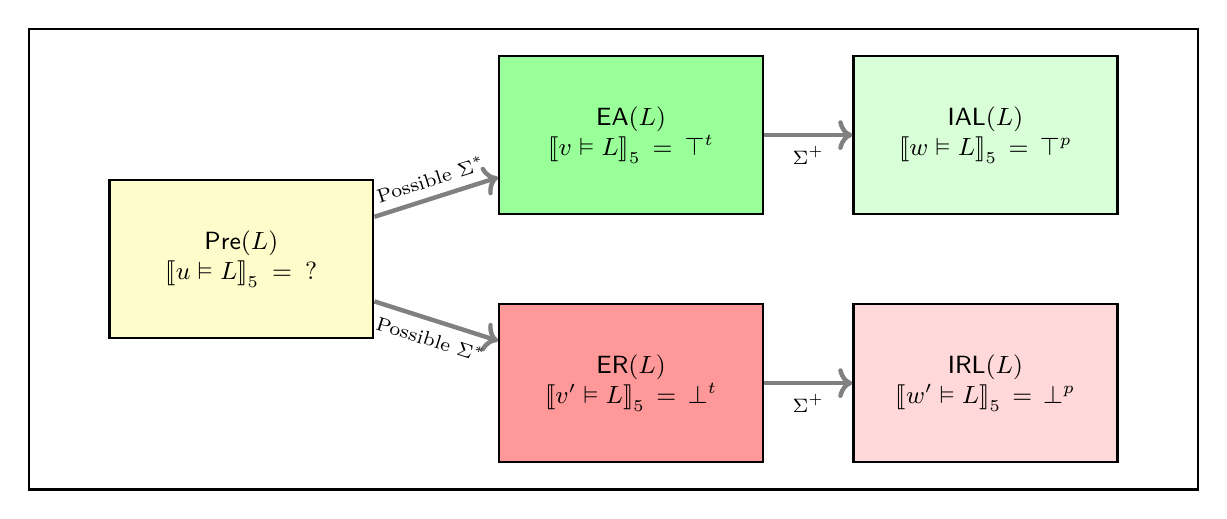
\begin{tikzpicture}[
      x=1cm, y=1cm, scale=0.9,
      every node/.style={font=\small\sffamily},
      % Region style: Fixed width and height for uniformity
      region/.style={draw, thick, fill opacity=1.0, align=center, inner sep=5pt, 
                     text width=3cm, minimum height=2cm}
  ]
  
      % --- Bounding Box ---
      % Adjusted width to fit the wider layout
      \draw[thick] (0,0) rectangle (16.5, 6.5);
      
  
      % --- Region: PRE (Centered vertically) ---
      \node[region, fill=yellow!20] (pre) at (3, 3.25) 
          {$\Pre{L}$ \\ $\semfive{u \vDash L}=\mathsf{?}$};

      % --- Column 2: Eager Frontiers ---
      % Shifted Right by 5.5cm

      % Eager Acceptance (Top Row)
      \node[region, fill=green!40] (eal) at (8.5, 5.0) 
          {$\EAL{L}$ \\ $\semfive{v \vDash L}=\topt$};

      % Eager Rejection (Bottom Row)
      \node[region, fill=red!40] (erl) at (8.5, 1.5) 
          {$\ERL{L}$ \\ $\semfive{v' \vDash L}=\bott$};

      % --- Column 3: Irrelevant Extensions ---
      % Shifted Right by 5cm

      % Irrelevant Acceptance (Top Row)
      \node[region, fill=green!15] (ial) at (13.5, 5.0) 
          {$\IAL{L}$ \\ $\semfive{w\vDash L}=\topp$};

      % Irrelevant Rejection (Bottom Row)
      \node[region, fill=red!15] (irl) at (13.5, 1.5) 
          {$\IRL{L}$ \\ $\semfive{w' \vDash L}=\botp$};
  
      % --- Bad Class Boundary (Dashed Red) ---
      % Encloses ERL and IRL (The bottom row)
  
      % --- Arrows ---
      \draw[->, ultra thick, gray] (pre) -- (eal) node[midway, sloped, above, font=\scriptsize, text=black] {Possible $\Sigma^*$};
      \draw[->, ultra thick, gray] (pre) -- (erl) node[midway, sloped, below, font=\scriptsize, text=black] {Possible $\Sigma^*$};
      \draw[->, ultra thick, gray] (eal) -- (ial) node[midway, sloped, below, font=\scriptsize, text=black] {$\Sigma^+$};
      \draw[->, ultra thick, gray] (erl) -- (irl) node[midway, sloped, below, font=\scriptsize, text=black] {$\Sigma^+$};
  
  \end{tikzpicture}
  \caption{Visualizing Theorem \ref{prop:tightness-obligations-unindexed}. We have either one of this evolution that is possible $u\prec v \prec w$ or $u\prec v' \prec w'$. The acceptance languages are in green and the rejection languages are in red. The diagram highlight possible extension of each language from the undecided prefix to the final verdict stages. The absence of an arrow between a language class to another implies that no direct evolution is possible.}
  \label{fig:five-way-partition}
\end{figure}




\subsubsection{From Language Automaton to Tight Monitor Construction}

This subsection explains how the deterministic language automaton obtained for a regular expression is lifted into a tight monitor. A language automaton recognises complete words of a regular expression, whereas a tight monitor must classify every prefix of every word into one of the five semantic regions. The transition structure of the automaton is therefore preserved, and only the output behaviour changes: each state receives a tight verdict according to the five-valued prefix semantics. This yields the tight monitor for regular expressions introduced in Definition~\ref{def:tsmc-re}.

We now recall the components used in this transformation and show how to convert the DFA into a Moore machine with tight verdicts.


\begin{definition}[Five-region automata]\label{def:five-aut}
Let $L\subseteq\Sigma^*$ be a regular language and let
\[
  \aut(L)=(Q,\Sigma,\delta,q_0,F)
  \quad\text{with}\quad \Lang{\aut(L)}=L
\]
be a DFA for $L$. We define the following DFAs, all over the same alphabet $\Sigma$:
\begin{itemize}
  \item $\aut_{\mathrm{EA}}(L)  := (Q_{\mathrm{EA}},\Sigma,\delta_{\mathrm{EA}},q^{0}_{\mathrm{EA}},F_{\mathrm{EA}})$
        with $\Lang{\aut_{\mathrm{EA}}(L)}=\EAL{L}$.
  \item $\aut_{\mathrm{PRE}}(L) := (Q_{\mathrm{PRE}},\Sigma,\delta_{\mathrm{PRE}},q^{0}_{\mathrm{PRE}},F_{\mathrm{PRE}})$
        with $\Lang{\aut_{\mathrm{PRE}}(L)}=\Pre{L}$.
  \item $\aut_{\mathrm{IAL}}(L) := (Q_{\mathrm{IAL}},\Sigma,\delta_{\mathrm{IAL}},q^{0}_{\mathrm{IAL}},F_{\mathrm{IAL}})$
        with $\Lang{\aut_{\mathrm{IAL}}(L)}=\IAL{L}$.
  \item $\aut_{\mathrm{ER}}(L)  := (Q_{\mathrm{ER}},\Sigma,\delta_{\mathrm{ER}},q^{0}_{\mathrm{ER}},F_{\mathrm{ER}})$
        with $\Lang{\aut_{\mathrm{ER}}(L)}=\ERL{L}$.
  \item $\aut_{\mathrm{IRL}}(L) := (Q_{\mathrm{IRL}},\Sigma,\delta_{\mathrm{IRL}},q^{0}_{\mathrm{IRL}},F_{\mathrm{IRL}})$
        with $\Lang{\aut_{\mathrm{IRL}}(L)}=\IRL{L}$.
\end{itemize}
\end{definition}

These DFAs are obtained using standard automata-theoretic constructions, including prefix-closure, complement, breadth-first identification of minimal accepting prefixes, and right-ideal saturation, as commonly used in DFA analysis as in \cite{HopcroftUllman2001}.

\begin{definition}[Five-region Moore machine]\label{def:five-moore}
Let $L\subseteq\Sigma^*$ be a regular language and let
\[
  \aut_{\mathrm{PRE}}(L),\,
  \aut_{\mathrm{EA}}(L),\,
  \aut_{\mathrm{ER}}(L),\,
  \aut_{\mathrm{IAL}}(L),\,
  \aut_{\mathrm{IRL}}(L)
\]
be the five DFAs from Definition~\ref{def:five-aut}, with accepting sets
$F_{\mathrm{PRE}},F_{\mathrm{EA}},F_{\mathrm{ER}},F_{\mathrm{IAL}},F_{\mathrm{IRL}}$.
The \emph{five-region Moore machine} for $L$ is the deterministic Moore machine
\[
  \mathcal{M}_{\text{5tight}}(L)
  \;:=\;
  \big(S,\ s^0,\ \Sigma,\ \tightverdicts,\ \delta,\ \lambda\big),
\]
where
\[
\begin{aligned}
S &:= Q_{\mathrm{PRE}}\times Q_{\mathrm{EA}}\times Q_{\mathrm{ER}}
      \times Q_{\mathrm{IAL}}\times Q_{\mathrm{IRL}},\\
s^0 &:= \big(q^0_{\mathrm{PRE}},\,q^0_{\mathrm{EA}},\,q^0_{\mathrm{ER}},\,
             q^0_{\mathrm{IAL}},\,q^0_{\mathrm{IRL}}\big),\\
\delta\!\big((p,e,r,a,\rho),\,\sigma\big)
&:= \big(\delta_{\mathrm{PRE}}(p,\sigma),\ \delta_{\mathrm{EA}}(e,\sigma),\
          \delta_{\mathrm{ER}}(r,\sigma),\
          \delta_{\mathrm{IAL}}(a,\sigma),\
          \delta_{\mathrm{IRL}}(\rho,\sigma)\big),\\
\lambda(p,e,r,a,\rho)
&:= \begin{cases}
      \topt & \text{if } e\in F_{\mathrm{EA}},\\
      \bott & \text{if } r\in F_{\mathrm{ER}},\\
      \topp & \text{if } a\in F_{\mathrm{IAL}},\\
      \botp & \text{if } \rho\in F_{\mathrm{IRL}},\\
      \mathsf{?} & \text{if } p\in F_{\mathrm{PRE}}.
    \end{cases}
\end{aligned}
\]
We write $\mathcal{M}_{\text{5tight}}(L)$ as a function of $L$, since $L$ uniquely determines
all components of this Moore machine.
\end{definition}



\begin{example}[Compact five-valued Moore monitor]
\label{ex:moore-tight-compact}
\small
The minimized five-output Moore machine for $L=\{a,ab,bb\}$ over $\Sigma=\{a,b\}$
produces $\tightverdicts=\{\mathsf{?},\topt,\bott,\topp,\botp\}$ according to the
unique accepting component among the five regions $\Pre{L}, \EAL{L}, \ERL{L}, \IAL{L}, \IRL{L}$.
\vspace{1ex}

\begin{figure}[h!]
\centering
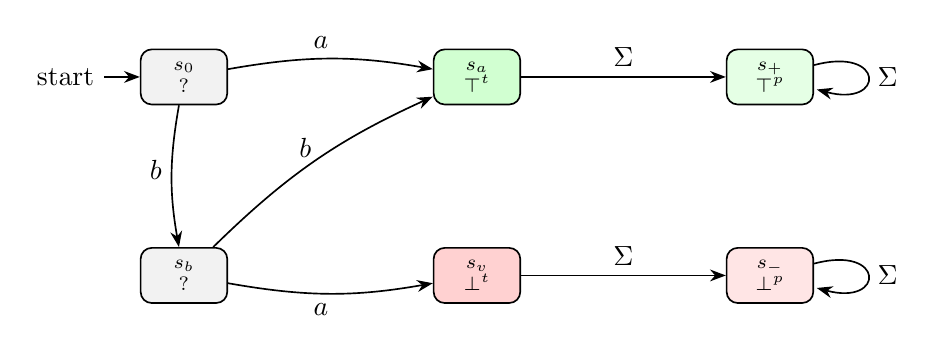
\begin{tikzpicture}[
  ->, >=Stealth, node distance=20mm, semithick,
  every state/.style={rectangle,rounded corners,draw,minimum width=11mm,
    minimum height=7mm,inner sep=2pt,font=\scriptsize,align=center}
]

% --- Nodes with embedded verdicts ---
\node[initial,state,fill=gray!10]    (s0) {$s_0$\\$\mathsf{?}$};
\node[state,fill=green!18,right=26mm of s0]  (sa) {$s_a$\\$\topt$};
\node[state,fill=green!10,right=26mm of sa]  (sp) {$s_+$\\$\topp$};
\node[state,fill=gray!10,below=18mm of s0]   (sb) {$s_b$\\$\mathsf{?}$};
\node[state,fill=red!18,below=18mm of sa]    (sv) {$s_v$\\$\bott$};
\node[state,fill=red!10,below=18mm of sp]    (sm) {$s_-$\\$\botp$};

% --- Transitions ---
\path
  (s0) edge[bend left=10] node[above,pos=0.45] {$a$} (sa)
       edge[bend right=10] node[left,pos=0.45]  {$b$} (sb)
  (sb) edge[bend left=10]  node[above,pos=0.45] {$b$} (sa)
       edge[bend right=10] node[below,pos=0.45]  {$a$} (sv)
  (sa) edge node[above] {$\Sigma$} (sp)
  (sv) edge node[above] {$\Sigma$} (sm)
  (sp) edge[loop right] node {$\Sigma$} ()
  (sm) edge[loop right] node {$\Sigma$} ();

\end{tikzpicture}
\caption{Minimized five-valued Moore machine for $L=\{a,ab,bb\}$.
Each node shows its name and output verdict ($\tightverdicts$).
Green states denote satisfaction, red denotes violation, and gray denotes undecided.
From $s_0$, input $a$ or $bb$ yields~$\topt$, input $ba$ yields~$\bott$,
and further inputs move to the post-frontier verdicts $\topp$ or $\botp$.}
\label{fig:moore-tight-compact}
\end{figure}
\end{example}


\begin{lemma}[Correctness of the tight-product Moore machine]\label{prop:five-moore-correct}
Let $L\subseteq\Sigma^*$ be regular and let $M_{\text{5tight}}(L)$ be as in
Definition~\ref{def:five-moore}. For every $u\in\Sigma^*$,
\[
\semfive{u \vDash L}\;=\;\lambda\!\big(\delta^{*}(s^0,u)\big),
\]
i.e., the output of $M_{\text{5tight}}(L)$ on input prefix $u$ coincides with the
five-valued semantics in Definition~\ref{def:five-valued-semantics}.
\end{lemma}

\begin{proof}
Let the five DFAs be
\[
\aut_{\mathrm{PRE}}(L),\quad
\aut_{\mathrm{EA}}(L),\quad
\aut_{\mathrm{ER}}(L),\quad
\aut_{\mathrm{IAL}}(L),\quad
\aut_{\mathrm{IRL}}(L),
\]
with recognized languages $\Pre{L}$, $\EAL{L}$, $\ERL{L}$, $\IAL{L}$, $\IRL{L}$, respectively.
By construction of $M_{\text{5tight}}(L)$, after reading $u$ the global state is
\[
\delta^{*}(s^0,u)
=\big(\delta_{\mathrm{PRE}}^{*}(q^{0}_{\mathrm{PRE}},u),\
      \delta_{\mathrm{EA}}^{*}(q^{0}_{\mathrm{EA}},u),\
      \delta_{\mathrm{ER}}^{*}(q^{0}_{\mathrm{ER}},u),\
      \delta_{\mathrm{IAL}}^{*}(q^{0}_{\mathrm{IAL}},u),\
      \delta_{\mathrm{IRL}}^{*}(q^{0}_{\mathrm{IRL}},u)\big).
\]
For each component DFA,
\[
\begin{aligned}
u\in\Pre{L}  &\iff \delta_{\mathrm{PRE}}^{*}(q^{0}_{\mathrm{PRE}},u)\in F_{\mathrm{PRE}},\\
u\in\EAL{L}  &\iff \delta_{\mathrm{EA}}^{*}(q^{0}_{\mathrm{EA}},u)\in F_{\mathrm{EA}},\\
u\in\ERL{L}  &\iff \delta_{\mathrm{ER}}^{*}(q^{0}_{\mathrm{ER}},u)\in F_{\mathrm{ER}},\\
u\in\IAL{L}  &\iff \delta_{\mathrm{IAL}}^{*}(q^{0}_{\mathrm{IAL}},u)\in F_{\mathrm{IAL}},\\
u\in\IRL{L}  &\iff \delta_{\mathrm{IRL}}^{*}(q^{0}_{\mathrm{IRL}},u)\in F_{\mathrm{IRL}}.
\end{aligned}
\]
By Theorem~\ref{thm:five-way}, the five languages form a pairwise-disjoint, complete partition of $\Sigma^*$. Hence, for each $u$ exactly one of the five memberships holds,
and $\lambda$ (by Definition~\ref{def:five-moore}) returns the unique verdict
of Definition~\ref{def:five-valued-semantics}. Therefore
$\lambda(\delta^{*}(s^0,u))=\semfive{u \vDash L}$.
\end{proof}


\begin{claim}[Linear-size Moore machine]\label{lem:moore-linear}
  Let $\aut(L)=(Q,\Sigma,\delta,q_0,F)$ be a completed DFA for $L$, and let
  $M_{\text{5tight}}(L)$ be the tight five-valued Moore machine of
  Definition~\ref{def:five-moore}.
  We assume that all five region DFAs in Definition~\ref{def:five-aut} are constructed
  over the same completed transition graph $(Q,\Sigma,\delta,q_0)$ of $\aut(L)$,
  differing only in their accepting sets.
  Then the number of reachable states of $M_{\text{5tight}}(L)$ is linear in the
  state space of $\aut(L)$, \ie, $|Q|$:
  \[
    \bigl|S_{\mathrm{reach}}(M_{\text{5tight}}(L))\bigr|
    \;=\;
    \bigl|\mathrm{Reach}(\aut(L))\bigr|
    \;\le\; |Q|.
  \]
  \end{claim}


  \paragraph{claim argument.}
  We argue directly from the constructions of the five DFAs used in $M_{\text{5tight}}(L)$. The validity of the linear size bound relies on the fact that all component automata are defined over the \emph{same underlying transition structure}.
  
  \smallskip
  \noindent
  \emph{(Invariant transition graph).}
  Starting from a completed DFA $\aut(L)=(Q,\Sigma,\delta,q_0,F)$, we construct the five region automata by modifying \emph{only} the accepting sets, while strictly preserving the transition graph $(Q,\Sigma,\delta)$. Crucially, we avoid standard minimization techniques that prune edges or merge states (such as making post-acceptance states sinks), as these would destroy the structural alignment required for the diagonal argument.
  \begin{itemize}
    \item The prefix-closure automaton $\closure{\aut(L)}$ uses $F_{\mathrm{PRE}} = \Live$ (states with a path to $F$).
    \item The bad-prefix automaton $\badc{\aut(L)}$ uses $F_{\mathrm{BAD}} = Q \setminus \Live$.
    \item The minimal-frontier automaton $\minc{\aut(L)}$ identifies the "first" accepting states without altering transitions.\\ We define $F_{\min} = \{ q \in F \mid \text{no predecessor of } q \text{ in the Bread First Search tree is in } F \}$. All outgoing edges from $F_{\min}$ remain intact, ensuring the graph topology is identical to $\aut(L)$.
    \item The right-ideal closures for $\IAL{L}$ and $\IRL{L}$ define their accepting sets by forward reachability from $F_{\min}$ and $F_{\min(\mathrm{Bad})}$ respectively, again without modifying $\delta$.
    \item Finally, $\ERL{L}$ is realized by the set difference $F_{\mathrm{ER}} := F_{\min(\mathrm{Bad})} \setminus F_{\mathrm{IAL}}$.
  \end{itemize}
  Thus, by construction, \emph{all five DFAs share the identical transition graph $(Q,\Sigma,\delta)$}.
  
  \smallskip
  \noindent
  \emph{(Diagonal runs in the product).}
  Fix any $u\in\Sigma^*$. Because the underlying transition function $\delta$ is identical across all five DFAs, the unique run from $q_0$ on $u$ ends in the \emph{same} state $q=\delta^*(q_0,u)$ in every component. Therefore, the reachable state space of the product Moore machine $M_{\text{5tight}}(L)$ is restricted exclusively to the diagonal:
  \[
  S_{\mathrm{reach}}(M_{\text{5tight}}(L)) \subseteq \{ (q,q,q,q,q) \mid q \in Q \}.
  \]
  
  \smallskip
  \noindent
  \emph{(Size bound).}
  The mapping $q \mapsto (q,q,q,q,q)$ defines a bijection between the reachable states of the original DFA and the reachable states of the tight Moore machine. Consequently:
  \[
       \bigl|S_{\mathrm{reach}}(\mathcal{M}_{\text{5tight}}(L))\bigr|
       \;=\;\bigl|\Reach(\aut(L))\bigr|
       \;\le\; |Q|.
  \]
  This proves that the size of the tight monitor is linear with respect to the input DFA, avoiding the state explosion typical of product constructions.
  
  Additionally, since each component DFA is deterministic and complete, $\mathcal{M}_{\text{5tight}}(L)$ is a deterministic Moore machine that emits exactly one verdict from $\tightverdicts$ for every prefix. The monotonic evolution of these verdicts is guaranteed by Theorem~\ref{prop:tightness-obligations-unindexed}.





Additionally, each component DFA is deterministic (and can be completed), so
$\mathcal{M}_{\text{5tight}}(L)$ itself is a deterministic Moore machine over $\Sigma$ that emits
exactly one verdict from $\tightverdicts=\{\mathsf{?},\topt,\bott,\topp,\botp\}$ for every
processed prefix. The evolution of verdicts along any word follows from
Theorem~\ref{prop:tightness-obligations-unindexed}: the output leaves $\mathsf{?}$ once to
either $\topt$ or $\bott$, and then remains in the corresponding post phase $\topp$ or $\botp$.

\paragraph*{Summary}
This section develops a \emph{correct-by-construction} toolkit that turns any regular language $L\subseteq\Sigma^*$ into the five semantic regions required by tight monitoring,
and then into a single monitor outputting all verdicts. The workflow relies only on classical automata-theoretic constructions, completion, product, complement, and breadth-first search on the DFA graph, used exactly as standard.

Starting from a DFA $\aut(L)$, we systematically build the prefix-closure automaton
$\closure{\aut(L)}$, which recognizes $\closureclass{L}$; its complement
$\badc{\aut(L)}$, which recognizes $\badclass{L}$; and the minimal-frontier automaton
$\minc{\aut(L)}$, which recognizes $\minlang{L}$. Two right-ideal saturations yield the
post regions $\IAL{L}$ and $\IRL{L}$, and one language difference realizes the
acceptance-first tie-break $\ERL{L} := \minlang{\badclass{L}}\setminus \IAL{L}$.

Practically, the approach is modular: each region is an ordinary DFA; scalable: construct only the reachable part of products and minimize components; and reusable across
specifications that share the same $L$. Conceptually, it aligns the linguistic requirements of normative systems, where norms enter into force at exact positions, with
executable monitors whose decisions are fair (no premature verdicts) and final
(no evolution to the opposite verdict). In short, standard automata technology, assembled carefully, delivers a monitor that is \emph{correct by design}.

\subsection{Illustration Through Regular Expressions from \cDL}
\label{subsec:re-tight}

This section demonstrates the process of defining monitors for regular expressions from \cDL. The procedure begins by specifying the language semantics of the regular expression, followed by a standard transformation into a deterministic automaton. Subsequently, the transformation described in the previous subsection is applied to construct the five tight semantic monitors for the formula.
This subsection fixes the semantics of the regular expressions that act as temporal guards in \cDL.

\subsubsection{Semantics for Regular Expressions from \cDL}
We work over the \emph{letter alphabet} $\Gamma := 2^{\Sigma_C^{(1)} \cup \Sigma_C^{(2)}}$ from the syntax in \ref{fig:cdl-syntax}, where each letter denotes the set of actions that occurred in one contractual period. 


\begin{definition}[Semantics of regular expressions]\label{def:re-semantics}
The satisfaction relation for a regular expression $\re$, written $\pi \modelsre \re$,
is defined over a finite trace $\pi=\langle A_0,\ldots,A_{n-1}\rangle\in\Gamma^*$,
where each letter $A_i\in\Gamma$ is a set of actions that occurred at period $i$.  
The relation is given inductively:
\[
\begin{array}{lcl}
\pi \modelsre \mathsf{A} &\text{iff}&  |\pi| = 1\ \text{and}\ \mathsf{A}\subseteq A_0,\\[4pt]
\pi \modelsre \Gamma &\text{iff}& |\pi| = 1,\\[4pt]
\emptytrace \modelsre \varepsilon, &\text{}& \\[4pt]
\pi \modelsre \emptyset &\text{iff}& A_0=\emptyset \nd |\pi| = 1,\\[4pt]
\pi \modelsre \re_1 \mid \re_2 &\text{iff}& (\pi \modelsre \re_1) \;\text{or}\; (\pi \modelsre \re_2),\\[4pt]
\pi \modelsre \re_1\cdot\re_2
&\text{iff}&
\exists k \in \{0,\dots,|\pi|\} :
\pi[0,k-1] \modelsre \re_1
\;\text{and}\;
\pi^{k} \modelsre \re_2,\\[4pt]
\pi \modelsre \re^1 &\text{iff}& \pi \modelsre \re,\\[4pt]
\pi \modelsre \re^n &\text{iff}& \pi \modelsre \re \cdot \re^{n-1} \text{ for } n>1,\\[4pt]
\pi \modelsre \re^+ &\text{iff}& 
  \exists\, n\ge1 : \pi \modelsre \re^n.
\end{array}
\]
We write $\Lang{\re} := \{\pi\in\Gamma^* \mid \pi \modelsre \re\}$ for the language of $\re$.
\end{definition}

\noindent
\noindent
{\emph{Reading the clauses.}}
\begin{itemize}
  \item \textbf{Atom $\mathsf{A}$.} Matches exactly one period: $\pi=\langle A_0\rangle$ with $\mathsf{A}\subseteq A_0$.
  \item \textbf{Wildcard $\Gamma$.} Matches any single period: $\pi=\langle A_0\rangle$ for arbitrary $A_0\in\Gamma$.
  \item \textbf{Empty word $\varepsilon$.} Matches only the empty word: $\pi= \emptytrace$.
  \item \textbf{Empty-action letter $\emptyset$.} Matches the one-period trace with no actions: $\pi=\langle \emptyset\rangle$.
  \item \textbf{Union $(re_1\mid re_2)$.} Holds iff at least one disjunct holds on the whole trace.
  \item \textbf{Sequencing $(re_1 \cdot re_2)$.}
There exists a split index $k$ such that
$\pi[0,k-1]\modelsre re_1$ and $\pi^{k}\modelsre re_2$.\footnote{The case $\pi[0,-1]$ is defined in \ref{traces} as $\emptytrace$}
  \item \textbf{Fixed power $re^n$.} Iterated sequencing of $re$ exactly $n$ times is inductively defined:
        two cases : if $n=1$ then evaluate for $re$; for $n>1$, enroll the first occurrence of $re$ and concatenate with $re^n-1$.
  \item \textbf{Kleene plus $re^+$.} Some positive iteration holds: $\exists n\ge1$ with $\pi\modelsre re^n$.
\end{itemize}
All satisfaction is defined on \emph{finite} traces, we show how to detect triggers and terminating conditions on regular expressions using the 5-valued semantics.





\subsubsection{Automata Construction Matching the Denotational Semantics}
\label{subsec:re-to-dfa}

We now give a concrete, standard pipeline that realizes the semantics of
Definition~\ref{def:re-semantics} \emph{exactly} by an automaton over the
alphabet $\Gamma=2^{\Sigma_C^{(1)}\cup\Sigma_C^{(2)}}$.

{\paragraph*{Stage 1  Thompson-style $\varepsilon$-NFA $\aut_{\varepsilon}(re)$ (alphabet-aware).}}
We build $\aut_{\varepsilon}(re)$ by structural recursion on $re$, using the
usual two distinguished states $(s_{\mathrm{in}},s_{\mathrm{out}})$ per fragment
and $\varepsilon$-transitions for wiring
(\cite{Thompson1968,HopcroftUllman2001,Sipser2012}). The only twist is how we
treat letters, since an atom $\mathsf{A}$ matches \emph{any} $\Gamma$-letter $X$
that \emph{covers} $\mathsf{A}$ (Definition~\ref{def:re-semantics}).

\begin{itemize}
  \item \textbf{Atom $\mathsf{A}\subseteq\Gamma$:} create two states
        $p\to q$ and add, for \emph{every} $X\in\Gamma$ with $\mathsf{A}\subseteq X$,
        a transition $p \xrightarrow{X} q$.
        This enforces “one period, with all actions in $\mathsf{A}$ present.”

  \item \textbf{Wildcard $\Gamma$:} create $p\xrightarrow{X} q$ for \emph{all} $X\in\Gamma$.

  \item \textbf{Empty word $\varepsilon$:} create $p \xrightarrow{\varepsilon} q$.

  \item \textbf{Empty-action letter $\emptyset$:} create a single-letter fragment
        $p \xrightarrow{\{\,\emptyset\,\}} q$ (i.e., only the $\Gamma$-letter $\emptyset$).

  \item \textbf{Union $(re_1 \mid re_2)$:} build fragments for $re_1$ and $re_2$ with
        entries/exits $(p_1,q_1)$ and $(p_2,q_2)$. Add fresh $p,q$ and wire
        $p \xrightarrow{\varepsilon} p_1$, $p \xrightarrow{\varepsilon} p_2$,
        $q_1 \xrightarrow{\varepsilon} q$, $q_2 \xrightarrow{\varepsilon} q$.

  \item \textbf{Sequencing $(re_1 \cdot re_2)$:} build $(p_1,q_1)$ and $(p_2,q_2)$, then
        add $q_1 \xrightarrow{\varepsilon} p_2$ and take $(p_1,q_2)$ as entry/exit.
        This matches the split $\pi[0,k]$ and $\pi[k{+}1,n]$ in the semantics.

  \item \textbf{Fixed power $re^n$:} unroll as $re;\cdots;re$ ($n$ times). The base
        $re^1\equiv re$.

  \item \textbf{Kleene plus $re^+$:} build $(p_1,q_1)$ for $re$, then add
        $q_1 \xrightarrow{\varepsilon} p_1$ and take $(p_1,q_1)$ as entry/exit.
        (At least one iteration is enforced by entering at $p_1$.)
\end{itemize}
Mark the global entry of the whole construction as initial, and the global exit as
accepting. The resulting NFA accepts exactly $\Lang{re}$.
\paragraph*{Stage 2  Determinization.}
Apply the standard subset construction with $\varepsilon$-closures to obtain a DFA $\aut_D(re)=(Q,\Gamma,\delta,q_0,F)$ that recognizes the same language, as demonstrated in
(\cite{RabinScott1959,HopcroftUllman2001}).

\paragraph*{Stage 3  Completion, trimming, and minimization.}
For monitoring we assume a \emph{completed} DFA: add (if needed) a sink state so that $\delta$ is total on $Q\times\Gamma$.
Next, trim unreachable states (retain only $\Reach(\aut_D(re))$).
Optionally, apply standard DFA minimization (for instance via partition refinement, as in Hopcroft's algorithm) to obtain an equivalent smallest DFA up to isomorphism.
This step is semantics-preserving and is used only to reduce the state space before the five-region constructions and the Moore lifting.


\paragraph*{Correctness (sketch).}
By structural induction on $re$. The letter fragments implement exactly the one-step clauses (\(\mathsf{A}\), $*$, $\emptyset$), union and sequencing are the usual
$\varepsilon$-wiring proofs, and $re^n$ (unrolled) and $re^+$ (loop back from the exit)
match the inductive clauses in Definition~\ref{def:re-semantics}. Determinization and completion preserve language.

\medskip
\noindent
\textbf{From $\aut(re)$ to the tight layers.}
Follow the same steps from Definition.~\ref{def:five-moore}:


\begin{example}[End-to-end construction]\label{ex:end-to-end-C5}
Continuing from Example.~\ref{ex:contract-encoding}, we demonstrate the automata construction for $C_5$:
\[
\begin{aligned}
\re_{C_5} &:= \Gamma^{+}\ \cdot \ \{\notifterm^{(1)}\}\ \cdot\ \Gamma^{3},\\
\Gamma    &:= 2^{\Sigma_C^{(1)} \cup \Sigma_C^{(2)}},\\
\Sigma_C  &:= \{\PAY,\ \PAYF,\ \OCC,\ \notifrepair,\ \notifterm,\ \REPAIR\}.
\end{aligned}
\]
Figure~\ref{fig:thompson-C5} depicts the Thompson-style $\varepsilon$-NFA for $\re_{C_5}$, and Figure~\ref{fig:dfa-C5-determinized} shows its determinized and completed DFA.

\tikzset{
  ->, >=Stealth,
  node distance=18mm,
  every state/.style={minimum size=24pt,inner sep=1pt,font=\small}
}

\begin{figure}[h]
\centering
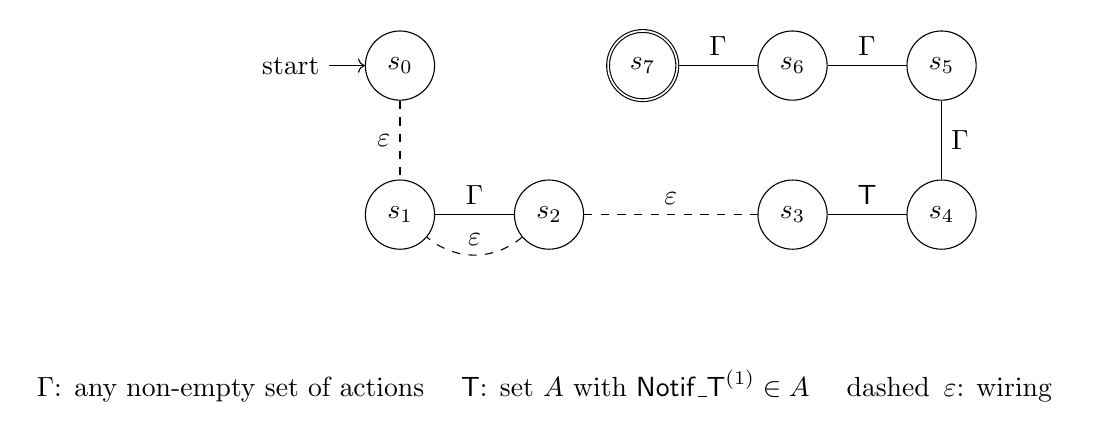
\begin{tikzpicture}
  % States
  \node[initial,state]            (s0) {$s_0$};
  \node[state,below=of s0]        (s1) {$s_1$};
  \node[state,right=of s1]        (s2) {$s_2$};
  %\node[state,right=14mm of s2]   (s1r) {$\,$}; % routing helper (invisible)
  \node[state,right=22mm of s2]   (s3) {$s_3$};
  \node[state,right=of s3]        (s4) {$s_4$};
  \node[state,above=of s4]        (s5) {$s_5$};
  \node[state,left=of s5]        (s6) {$s_6$};
  \node[state,accepting,left=of s6] (s7) {$s_7$};

  % Epsilon wiring: entry to + loop region
  \path (s0) edge[dashed] node[left] {$\varepsilon$} (s1);
  % + block: at least one Γ then possibly repeat (Thompson for re^+)
  \path (s1) edge node[above] {$\Gamma$} (s2);
  \path (s2) edge[dashed,bend left=40] node[above] {$\varepsilon$} (s1);

  % Move from the + block to the atom {notifterm^(1)}
  \path (s2) edge[dashed] node[above] {$\varepsilon$} (s3);
  % The atom itself: a single letter that contains notifterm^(1)
  \path (s3) edge node[above] {$\mathsf{T}$} (s4);

  % Then exactly 3 wildcards (three periods)
  \path (s4) edge node[right] {$\Gamma$} (s5);
  \path (s5) edge node[above] {$\Gamma$} (s6);
  \path (s6) edge node[above] {$\Gamma$} (s7);

  % Legend (optional, small)
  \node[below=14mm of s2,align=center] (leg) {%
    $\Gamma$: any non-empty set of actions \quad
    $\mathsf{T}$: set $A$ with $\notifterm^{(1)}\in A$ \quad
    dashed $\,\varepsilon$: wiring
  }
  ;
\end{tikzpicture}
\caption{Thompson-style $\varepsilon$-NFA for
$\re_{C_5} = \Gamma^{+} \cdot  \{\notifterm^{(1)}\} \cdot \Gamma^{3}$ over $\Gamma=2^{\Sigma}$.
From $s_0$ we enter the $\Gamma^{+}$ block ($s_1 \xrightarrow{\Gamma} s_2$ with a back
$\varepsilon$-loop to enforce “one or more” steps), then take a single
$\mathsf{T}$-labeled letter (the period that contains $\notifterm^{(1)}$),
followed by exactly three arbitrary periods (three $\Gamma$ transitions) to the
accepting state $s_7$. Determinization and completion of this NFA yield a DFA
that recognizes precisely the denotation of $\re_{C_5}$ in
Definition~\ref{def:re-semantics}.}
\label{fig:thompson-C5}
\end{figure}

\begin{figure}
\centering
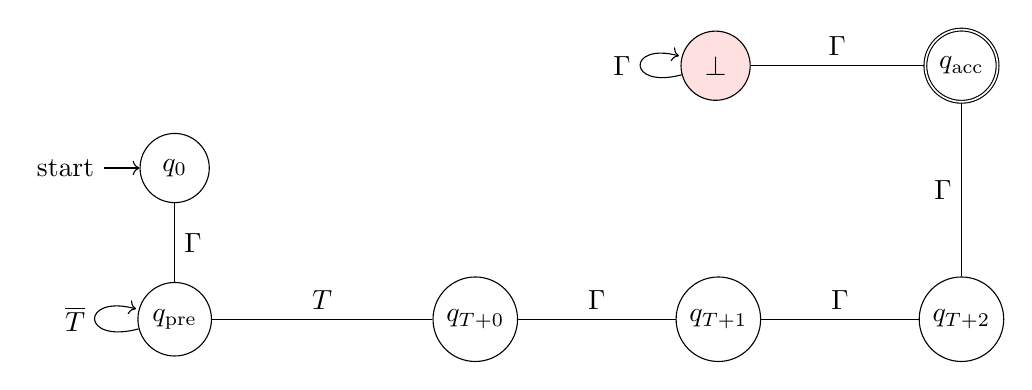
\begin{tikzpicture}
  % States
  \node[initial,state]             (q0) {$q_0$};                 % start: 0 letters so far
  \node[state,below=of q0]         (qpre) {$q_{\text{pre}}$};    % consumed ≥1 letter, before the middle T
  \node[state,right=28mm of qpre]  (qT0) {$q_{T+0}$};            % just saw the middle T, need 3 more
  \node[state,right=20mm of qT0]   (qT1) {$q_{T+1}$};            % need 2 more
  \node[state,right=20mm of qT1]   (qT2) {$q_{T+2}$};            % need 1 more
  \node[state,accepting,above=22mm of qT2] (qAcc) {$q_{\mathrm{acc}}$}; % done: exactly 3 after T
  \node[state,fill=red!12,left=22mm of qAcc] (sink) {$\bot$};     % sink for any overrun / dead move

  % Transitions
  % From q0: first letter must be in \Gamma^+, so any \Gamma goes to pre
  \path (q0) edge node[right] {$\Gamma$} (qpre);

  % In q_pre: keep consuming \Gamma^+ by non-T (stay), or take the middle T to enter the tail counter
  \path (qpre) edge[loop left] node {$\overline{T}$} ()
              edge node[above] {$T$} (qT0);

  % After the middle T: count exactly 3 more letters (any)
  \path (qT0) edge node[above] {$\Gamma$} (qT1);
  \path (qT1) edge node[above] {$\Gamma$} (qT2);
  \path (qT2) edge node[left]  {$\Gamma$} (qAcc);

  % From accepting, any further letter overruns → sink; sink loops
  \path (qAcc) edge node[above] {$\Gamma$} (sink);
  \path (sink) edge[loop left] node {$\Gamma$} ();

\end{tikzpicture}
\caption{Determinized and completed DFA for \(\re_{C_5}=\Gamma^{+}\cdot\{\notifterm^{(1)}\}\cdot\Gamma^{3}\) over the alphabet \(\Gamma=2^{\Sigma}\).
State \(q_{\text{pre}}\) collects the initial $\Gamma^{+}$ segment; transition on \(T\) begins
the “+3 letters” counter (\(q_{T+0}\to q_{T+1}\to q_{T+2}\to q_{\mathrm{acc}}\)).
Any overrun moves to the sink.}
\label{fig:dfa-C5-determinized}
\end{figure}
\end{example}



We now close the pipeline from guards to monitors.
Starting from a regular expression $\re$ in \cDL, we have fixed its denotational language $\Lang{\re}\subseteq\Gamma^*$ (Definition~\ref{def:re-semantics}) and we can obtain a completed DFA for this language by the standard NFA-to-DFA constructions.
What remains is to turn this language recognizer, which only decides membership of whole words, into an executable artefact that classifies \emph{every prefix} according to the tight regions introduced earlier.
The construction below performs exactly this lift: it wraps $\Lang{\re}$ into the five-region Moore machine and thereby yields a tight satisfaction monitor whose output coincides with the five-valued prefix semantics on all prefixes.

\subsubsection{From Language Automaton to Tight Monitor Construction}\label{subsec:re-to-monitor}

\begin{definition}[Tight monitor construction for regular expressions]\label{def:tsmc-re}
Let $\re$ be a regular expression over the alphabet $\Gamma$ and let
$L := \Lang{\re}\subseteq\Gamma^{*}$ be its language as in Definition~\ref{def:re-semantics}.
Let
\[
  \mathcal{M}_{\text{5tight}}(L)
  \;=\;\big(S, s^0, \Gamma, \tightverdicts, \delta, \lambda\big)
\]
be the five-region Moore machine for $L$ from Definition~\ref{def:five-moore}.
The \emph{tight satisfaction monitor} for $\re$ is this Moore machine:
\[
  \tsmc_{\re}(\re) \;:=\; \mathcal{M}_{\text{5tight}}(\Lang{\re}).
\]
\end{definition}

By construction, for every prefix $u\in\Gamma^{*}$, the output of $\tsmc_{\re}(\re)$ after reading $u$
coincides with the tight five-valued semantics:
\[
  \lambda\big(\delta(s^0,u)\big) \;=\; \semfive{u \vDash \Lang{\re}}.
\]

\begin{example}[Tight monitor for $C_5$]\label{ex:moore-C5-tight}
Continuing Example~\ref{ex:end-to-end-C5}, Figure~\ref{fig:moore-C5-tight-compact} shows the compact five-valued Moore monitor obtained by applying the tight monitor construction of Definition~\ref{def:tsmc-re} to the regular expression $\re_{C_5}$.
\begin{figure}[h!]
\centering
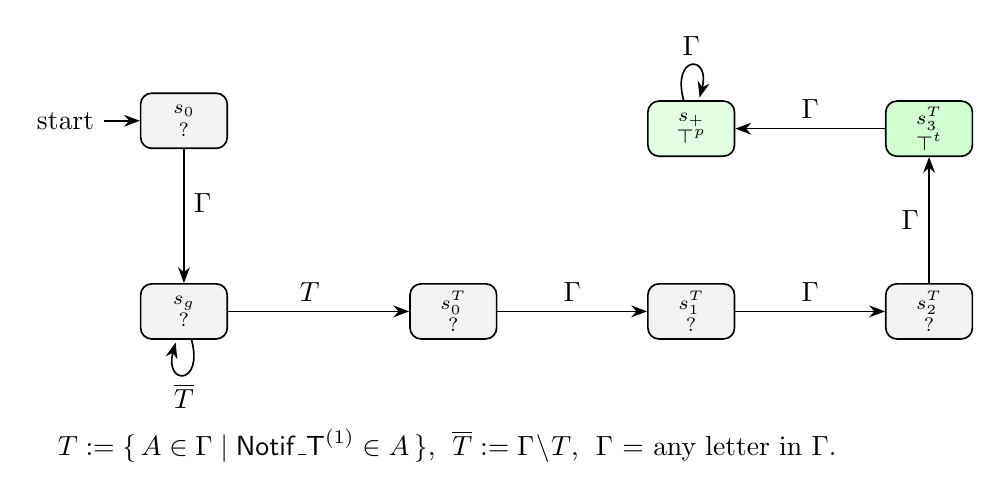
\begin{tikzpicture}[
  ->, >=Stealth, node distance=17mm, semithick,
  every state/.style={rectangle,rounded corners,draw,
    minimum width=11mm,minimum height=7mm,
    inner sep=2pt,font=\scriptsize,align=center}
]

% --- Nodes with embedded verdicts ---
\node[initial,state,fill=gray!10]  (s0)  {$s_0$\\$\mathsf{?}$};
\node[state,fill=gray!10,below=of s0]  (g)   {$s_g$\\$\mathsf{?}$};
\node[state,fill=gray!10,right=23mm of g] (t0) {$s_0^T$\\$\mathsf{?}$};
\node[state,fill=gray!10,right=19mm of t0] (t1) {$s_1^T$\\$\mathsf{?}$};
\node[state,fill=gray!10,right=19mm of t1] (t2) {$s_2^T$\\$\mathsf{?}$};
\node[state,fill=green!18,above=16mm of t2] (acc) {$s_3^T$\\$\topt$};
\node[state,fill=green!10,left=19mm of acc] (ap) {$s_{+}$\\$\topp$};

% --- Transitions ---
\path
  (s0) edge node[right,pos=0.4] {$\Gamma$} (g)
  (g) edge[loop below] node {$\overline{T}$} ()
  (g) edge node[above,pos=0.45] {$T$} (t0)
  (t0) edge node[above,pos=0.5] {$\Gamma$} (t1)
  (t1) edge node[above,pos=0.5] {$\Gamma$} (t2)
  (t2) edge node[left,pos=0.5] {$\Gamma$} (acc)
  (acc) edge node[above,pos=0.5] {$\Gamma$} (ap)
  (ap) edge[loop above] node {$\Gamma$} ();

% --- Legend ---
\node[below=10mm of t0,align=center] (leg){
$T := \{\,A\in\Gamma\mid \notifterm^{(1)}\in A\,\}$,\;
$\overline{T} := \Gamma\!\setminus\! T$,\;
$\Gamma$ = any letter in $\Gamma$.
};

\end{tikzpicture}
\caption{Compact five-valued Moore monitor for
$re_{C_5}=\Gamma^{+} \cdot \{\notifterm^{(1)}\} \cdot \Gamma^{3}$.
} 
\label{fig:moore-C5-tight-compact}
\end{figure}

\end{example}


\section{Tight Forward Reasoning on Contract Compliance}

\paragraph{Methodological overview.}
This section develops the forward-looking semantics and monitoring constructions in a layered manner.
We first introduce tight satisfaction and violation as \emph{frontier-based} judgements over prefixes of a synchronous periodic trace.
These judgements identify the unique decisive point at which a contract becomes irrevocably satisfied or violated.
On top of this core semantics, we derive coarser verdicts, prove coherence properties, and construct Moore-style monitors that operationalize the semantics.
The continuation of this development extends the same methodology to responsibility-aware verdicts and blame monitoring.
\subsection{Denotational Semantics for Forward-Looking Tight Contract Satisfaction}\label{forwardsatsem}
Fix the tagged collaboration alphabet $\Sigma = \Sigma_C^{(1)} \cup \Sigma_C^{(2)}$
and the induced letter alphabet $\Gamma = 2^{\Sigma}$.
Traces, prefixes, suffixes, and their basic operators are as defined in
\ref{traces}.
In this subsection, we only introduce the forward-looking semantic
judgements used to evaluate contracts along such traces.

\medskip
\paragraph{Core tight judgements.}
All semantic clauses below are stated relative to the prefix structure
fixed in \ref{traces}.

We define two tight relations (inductively on the syntax of $C$):
\[
\pi\ \satt\ C \quad\text{(tight satisfaction)},\qquad
\pi\ \violt\ C \quad\text{(tight violation)}.
\]
Intuitively, $\satt$ holds exactly at the \emph{first prefix}
where the contract becomes satisfied (acceptance frontier),
and $\violt$ holds exactly at the \emph{first prefix}
where it becomes violated (rejection frontier).

\medskip
\paragraph{Derived judgements.}
Using these frontiers, we define the remaining derived relations of the five-valued semantics.
By Lemma~\ref{lem:mutual prefix}, at most one tight frontier can occur along a fixed trace, so the clauses below classify a prefix by its position relative to this (unique, if it exists) decisive point.

\begin{definition}[Post and Pre-satisfaction semantic definition]\label{def:postprecont}
For a contract $C$ and trace $\pi$ the Pre satisfaction relation $\presat$, the post satisfaction and violation relations, respectively $\postsat$ and $\postviol$ are defined on the structure of the trace $\pi$ and the tight satisfaction and violation relations:
\[
\begin{array}{rcl}
\pi\ \presat\ C
&\iff&
\forall\,k<|\pi|:\ \neg\big(\pi[1,k]\ \satt\ C\big)\ \nd\ \neg\big(\pi[1,k]\ \violt\ C\big),
\\[0.8ex]
\pi\ \postsat\ C
&\iff&
\exists\,k<|\pi|:\ \pi[1,k]\ \satt\ C,
\\[0.8ex]
\pi\ \postviol\ C
&\iff&
\exists\,k<|\pi|:\ \pi[1,k]\ \violt\ C.
\end{array}
\]
\end{definition}
Each trace prefix is classified relative to the earliest decisive prefix: before it the trace is undecided ($\presat$), at it the contract is decided tightly ($\satt$ or $\violt$), and after it the trace is beyond the decision frontier ($\postsat$ or $\postviol$).
The fact that these five regions are pairwise disjoint and jointly exhaustive is established formally in Theorem~\ref{thm:five-partition}.

\medskip
\paragraph{Collapsed two-valued judgements.}
For downstream use (e.g., compliance checking), we collapse the five tight judgements into a two-valued view.
For conservativeness, undecided prefixes are treated as violating, which prevents premature acceptance.
\[
\begin{array}{rcl}
\pi \models_\top \ C
&\iff&
\big(\pi\ \satt\ C\big)\ \sor\ \big(\pi\ \postsat\ C\big),
\\[0.6ex]
\pi\ \viol\ C
&\iff&
\big(\pi\ \presat\ C\big)\ \sor\ \big(\pi\ \violt\ C\big)\ \sor\ \big(\pi\ \postviol\ C\big).
\end{array}
\]
Exactly one of $\pi\ \sat\ C$ or $\pi\ \viol\ C$ holds for every trace~$\pi$ and contract~$C$.
This conservative collapse treats undecided prefixes as \emph{violating}
(no premature acceptance) while still preserving the tight moment of satisfaction.

\subsubsection*{Literal Tight Semantics}
Literals $\ell$ are decided in a single synchronous step.
We therefore interpret them on a single event word $\trace{A}$ with $A\in\Gamma$
(the set of actions that occurred in one period).

\par
We present the literal clauses for party $p=1$; the case $p=2$ is symmetric (by swapping $(\cdot)^{(1)}$ and $(\cdot)^{(2)}$).

Intuitively, for party~1:
(i) an \emph{obligation} $\obl[1]{a}$ requires the joint execution of $a^{(1)}$ and $a^{(2)}$;
(ii) a \emph{prohibition} $\frb[1]{a}$ is satisfied precisely when that joint execution does not occur; and
(iii) a \emph{power} $\perm[1]{a}$ requires that whenever party~1 attempts $a^{(1)}$,
party~2 simultaneously supports it with $a^{(2)}$.

%
\begin{definition}[Literal tight satisfaction]\label{def:lattsat}
  For the empty trace, we have:
  \[
  \emptytrace\ \presat \ell \quad \text{for any literal } \ell.
  \]
  Literals are decided on a single synchronous step. We define their semantics on a single event word $\trace{A}$ ($A\in\Gamma$) and the empty word $\emptytrace$.
  \[
  \emptytrace\ \presat \ell \quad \text{for any literal } \ell.
  \]
  \smallskip
  \noindent\textbf{Tight satisfaction.}
  For a single event word $\trace{A}$:
  \[
  \begin{array}{l@{\quad}c@{\quad}l}
  \trace{A}\ \satt\ \top      &\mydef& \text{true}.\\[4pt]
  \trace{A}\ \satt\ \bot      &\mydef& \text{false}.\\[6pt]
  \trace{A}\ \satt\ \obl[1]{a} &\mydef& \{a^{(1)},a^{(2)}\}\subseteq A.\\[6pt]
  \trace{A}\ \satt\ \frb[1]{a} &\mydef& \{a^{(1)},a^{(2)}\}\not\subseteq A.\\[6pt]
  \trace{A}\ \satt\ \perm[1]{a} &\mydef& \text{if }(a^{(1)}\in A) \text{ then }(a^{(2)}\in A).
  \end{array}
  \]
  
  \medskip
  
  \noindent\textbf{Tight violation.}
  For a single event word $\trace{A}$:
  \[
  \begin{array}{l@{\quad}c@{\quad}l}
  \trace{A}\ \violt\ \top      &\mydef& \text{false}.\\[4pt]
  \trace{A}\ \violt\ \bot      &\mydef& \text{true}.\\[6pt]
  \trace{A}\ \violt\ \obl[1]{a} &\mydef& \{a^{(1)},a^{(2)}\}\not\subseteq A.\\[6pt]
  \trace{A}\ \violt\ \frb[1]{a} &\mydef& \{a^{(1)},a^{(2)}\}\subseteq A.\\[6pt]
  \trace{A}\ \violt\ \perm[1]{a} &\mydef& (a^{(1)}\in A) \nd (a^{(2)}\notin A).
  \end{array}
  \]
  \end{definition}

\begin{example}[Literal satisfaction and violation]
Let $A=\{a^{(1)},a^{(2)},b^{(2)}\}$ be the joint actions in one period.
Then
\[
\trace{A}\ \satt\ \obl[1]{a},\qquad
\trace{A}\ \satt\ \perm[1]{a},\qquad
\trace{A}\ \satt\ \frb[2]{b}.
\]
Let $A'=\{a^{(1)},b^{(1)},b^{(2)}\}$. Then
\[
\trace{A'}\ \violt\ \perm[1]{a}\quad\text{(since $a^{(2)}\notin A'$)},\qquad
\trace{A'}\ \satt\ \frb[2]{a}\quad\text{(no joint $a^{(1)} \nd a^{(2)}$ occurs).}
\]
Also, $\trace{A'}\ \satt\ \perm[2]{a}$ holds vacuously since $a^{(2)}\notin A'$.

\medskip
\noindent\textbf{Two-event trace.}
Consider $\trace{A,A'}$.
Since literals are decided at the first letter,
the overall collapsed verdict follows from $\trace{A}$ are post satisfaction or post violation:
\[
\begin{array}{l}
\trace{A,A'}\ \postsat\ \obl[1]{a},\\[4pt]
\trace{A,A'}\ \postsat\ \perm[1]{a},\\[4pt]
\trace{A,A'}\ \postviol\ \perm[2]{b}.
\end{array}
\]
\end{example}

\subsubsection*{Binary Contract Operators Tight Semantics}
\label{sec:tight-binary}
Binary contract operators combine two contracts into structured compositions that capture
parallel, sequential, or conditional behavior.  
In \cDL\ we use
\[
\textsf{op} \in \{\wedge,\ ;\ ,\ \repair\},
\]
where $\wedge$ enforces \emph{both} components, $;$ demands \emph{first $C$ then $C'$},
and $\repair$ means “if $C$ fails, \emph{repair} with $C'$.”

\medskip
\noindent\textbf{Reading guide (tight view).}
All clauses below are tight: they identify the \emph{first decisive point}
where satisfaction or violation becomes determined.
For conjunction, the decisive point for satisfaction is the latter of the two individual successes; for violation, the first conjunct that fails.
For sequencing, a split index $k$ witnesses that $C$ succeeds before $C'$ is checked.
Reparation, on the other hand, requires that either $C$ succeeds directly, or, at the first tight violation of $C$, the repair $C'$ must succeed on the remainder.

\begin{definition}[Binary Contract Operators]
  \label{def:binary-contract-semantics}
  Let $\pi$ be a finite trace over $\Gamma = 2^{\Sigma}$ with  $s=\size{\pi}$.
  We use the notation $\pi_k = \pi[1,k]$ for the prefix of length $k$,
  and $\pi^k = \pi[k+1,s]$ for the suffix after $k$.

  \[
  \begin{array}{l@{\quad}c@{\quad}l}
  \multicolumn{3}{l}{\textbf{Conjunction }(C \wedge C')}\rule{0pt}{2.4ex}\\
  \pi\ \satt\ C \wedge C'
  &\mydef&
  \exists\,k,k' \in [1,s]:\
  \pi_{k}\ \satt\ C\ \nd\
  \pi_{k'}\ \satt\ C'\ \nd\ \\
  & &s=\max(k,k'),
  \\[1.2ex]
  \pi\ \violt\ C \wedge C'
  &\mydef&
  (\pi\ \violt\ C\ \sor\ \pi\ \violt\ C')\ \nd\ \\
  & &\forall\,j \in [1, s-1]:\ \lnot(\pi_{j}\ \violt\ (C \wedge C')),
  \\[2ex]

  \multicolumn{3}{l}{\textbf{Sequence }(C\ ;\ C')}\rule{0pt}{2.4ex}\\
  \pi\ \satt\ C ; C'
  &\mydef&
  \exists\,k \in [1, s-1]:\ \pi_k\ \satt\ C\ \nd\ \pi^{k}\ \satt\ C',
  \\[1.2ex]
  \pi\ \violt\ C ; C'
  &\mydef&
  \pi\ \violt\ C\ \sor\
  \exists\,k \in [1, s-1]:\ \pi_k\ \satt\ C\ \nd\ \pi^{k}\ \violt\ C',
  \\[2ex]

  \multicolumn{3}{l}{\textbf{Reparation }(C\ \repair\ C')}\rule{0pt}{2.4ex}\\
  \pi\ \satt\ C \repair C'
  &\mydef&
  \pi\ \satt\ C\ \sor\
  \exists\,k \in [1, s-1]:\ \pi_k\ \violt\ C\ \nd\ \pi^{k}\ \satt\ C',
  \\[1.2ex]
  \pi\ \violt\ C \repair C'
  &\mydef&
  \exists\,k \in [1, s-1]:\ \pi_k\ \violt\ C\ \nd\ \pi^{k}\ \violt\ C'.
  \end{array}
  \]
\end{definition}

\paragraph{Semantics summary.}
\emph{Conjunction} succeeds once both parts succeed (possibly at different times); its decisive index is the latter of the two.  
It fails as soon as either part fails.  
\emph{Sequence} requires a witness split $k$:
first $C$ succeeds on $[1,k]$, then $C'$ on $[k{+}1,s]$.
\emph{Reparation} allows $C'$ to take over at the first violation of $C$; overall success means either direct success of $C$
or a violation-then-repair pattern.


\begin{lemma}[Local disjointness of tight satisfaction and violation for binary operators]
  \label{lem:binary-disjoint}
  Let $C,C'$ be contracts and let $\pi$ be a finite trace. Assume the following
  induction hypotheses hold for the subcontracts:
  \[
  \neg\bigl(\pi \satt C \ \nd\ \pi \violt C\bigr)
  \qquad\text{and}\qquad
  \neg\bigl(\pi \satt C' \ \nd\ \pi \violt C'\bigr),
  \]
  and, moreover, the same disjointness holds for every suffix $\pi^{k}$ in place of $\pi$.
  Then, for each binary operator $\textsf{op}\in\{\wedge,\ ;\ ,\ \repair\}$ we have
  \[
  \neg\bigl(\pi \satt (C\ \textsf{op}\ C') \ \nd\ \pi \violt (C\ \textsf{op}\ C')\bigr).
  \]
  \end{lemma}
  
  \begin{proof}
    We prove the three cases by contradiction, using Definition~\ref{def:binary-contract-semantics}.
    We also use Lemma~\ref{lem:mutual prefix} to rule out an opposite frontier on a strict prefix once a tight verdict holds on the full trace.
    
    \paragraph{Case $\wedge$.}
    Assume $\pi \satt (C\wedge C')$ and $\pi \violt (C\wedge C')$.
    From $\pi \satt (C\wedge C')$ there exist $k,k'\in[1,s]$ such that
    $\pi_k \satt C$, $\pi_{k'} \satt C'$, and $s=\max(k,k')$.
    From $\pi \violt (C\wedge C')$ we obtain $\pi \violt C$ or $\pi \violt C'$.
    
    If $\pi \violt C$, then:
    (i) if $k=s$, we have $\pi \satt C$ and $\pi \violt C$, contradicting the disjointness hypothesis for $C$;
    (ii) if $k<s$, then $\pi_k$ is a strict prefix of $\pi$ with $\pi_k \satt C$, contradicting Lemma~\ref{lem:mutual prefix}(2) instantiated with $C$ (since $\pi \violt C$ forbids any $j<s$ with $\pi_j \satt C$).
    The case $\pi \violt C'$ is symmetric.
    
    \paragraph{Case $;$.}
    Assume $\pi \satt (C;C')$ and $\pi \violt (C;C')$.
    From satisfaction there exists $k\in[1,s-1]$ such that
    $\pi_k \satt C$ and $\pi^{k} \satt C'$.
    From violation either (i) $\pi \violt C$ or (ii) there exists $m\in[1,s-1]$ such that
    $\pi_m \satt C$ and $\pi^{m} \violt C'$.
    
    In case (i), $\pi \violt C$ contradicts Lemma~\ref{lem:mutual prefix}(2) for $C$
    because $\pi_k$ is a strict prefix with $\pi_k \satt C$.
    
    In case (ii), tight satisfaction of $C$ is a frontier event along prefixes of a fixed trace,
    so $\pi_k \satt C$ and $\pi_m \satt C$ imply $k=m$.
    Hence, the same suffix $\pi^{k}$ both tightly satisfies and tightly violates $C'$,
    namely $\pi^{k} \satt C'$ and $\pi^{k} \violt C'$,
    contradicting the suffix-disjointness hypothesis for $C'$.
    
    \paragraph{Case $\repair$.}
    Assume $\pi \satt (C\repair C')$ and $\pi \violt (C\repair C')$.
    From $\pi \violt (C\repair C')$ there exists $k\in[1,s-1]$ such that
    $\pi_k \violt C$ and $\pi^{k} \violt C'$.
    From $\pi \satt (C\repair C')$ either (a) $\pi \satt C$ or (b) there exists $m\in[1,s-1]$ such that
    $\pi_m \violt C$ and $\pi^{m} \satt C'$.
    
    In case (a), $\pi \satt C$ and the strict-prefix violation $\pi_k \violt C$ contradict
    Lemma~\ref{lem:mutual prefix}(1) instantiated with $C$.
    
    In case (b), tight violation of $C$ is also a frontier event along prefixes of a fixed trace,
    so $\pi_k \violt C$ and $\pi_m \violt C$ imply $k=m$.
    Hence, the same suffix $\pi^{k}$ both violates and satisfies $C'$,
    namely $\pi^{k} \violt C'$ and $\pi^{k} \satt C'$,
    contradicting the suffix-disjointness hypothesis for $C'$.
    
    Thus in all three cases we reach a contradiction, so
    $\neg\bigl(\pi \satt (C\ \textsf{op}\ C') \ \nd\ \pi \violt (C\ \textsf{op}\ C')\bigr)$.
    \end{proof}



\begin{example}[Tight satisfaction and violation for $(C_2 \wedge C_3)$]
\label{ex:c2c3-tight}
We reuse the collaboration alphabet
\[
\Sigma_C=\{\PAY,\ \PAYF,\ \OCC,\ \notifrepair,\ \REPAIR\},
\]
and recall
\[
C_2 := \perm[1]{\OCC}, \qquad
C_3 := \obl[1]{\PAY}\ \repair\ \obl[1]{\PAYF}.
\]

\paragraph{Tight satisfaction (the longest prefix).}
Consider the trace
\[
\pi_{\textsf{sat}} = \langle A_1, A_2\rangle,
\qquad
A_1=\{\OCC^{(2)}\},\quad
A_2=\{\PAYF^{(1)},\PAYF^{(2)}\}.
\]
Then
$\trace{A_1}\ \satt\ C_2$
(vacuously, since $\OCC^{(1)}\notin A_1$ and no unsupported attempt occurs),
and
$\pi_{\textsf{sat}}\ \satt\ C_3$
(the rent was not paid in month 1, but the reparation clause succeeds at $t{=}1$).
Hence, by conjunction,
$\pi_{\textsf{sat}}\ \satt\ (C_2 \wedge C_3)$
at the longest decisive prefix.

\paragraph{Tight satisfaction (the shortest prefix).}
For the single-event trace 
\[
\trace{A_1'} \quad\text{with}\quad A_1'=\{\OCC^{(2)},\PAY^{(1)},\PAY^{(2)}\},
\]
we have
$\trace{A_1'}\ \satt\ C_2$
and
$\trace{A_1'}\ \satt\ \obl[1]{\PAY}$,
so both conjuncts hold in month 1:
\[
\trace{A_1'}\ \satt\ (C_2 \wedge C_3),
\quad
\text{and any extension }\trace{A_1',A_2}\text{ yields }\postsat(C_2\wedge C_3).
\]

\paragraph{Tight violation.}
Now consider
\[
\pi_{\textsf{viol}} = \langle A_1, A_2\rangle,
\qquad
A_1=\{\OCC^{(1)}\},\quad
A_2=\emptyset.
\]
In the first month,
$\trace{A_1}\ \satt\ C_2$
and $\trace{A_1}\ \violt\ \obl[1]{\PAY}$,
while
$\trace{A_1}\ \presat\ C_3$
since the reparation in $C_3=\obl[1]{\PAY}\repair\obl[1]{\PAYF}$ has not yet been tested.
At $t{=}1$,
$\pi_{\textsf{viol}}\ \violt\ C_3$
(as $\pi[1,1]\ \violt\ \obl[1]{\PAY}$ and $\pi[2,2]\ \violt\ \obl[1]{\PAYF}$).
Thus, the overall violation arises from $C_3$,
and by conjunction,
$\pi_{\textsf{viol}}\ \violt\ (C_2 \wedge C_3)$.

\medskip
This shows that $(C_2 \wedge C_3)$
satisfies either immediately when both conjuncts hold, or later when a reparation compensates for a missed rent, while violation arises when both payment and its repair fail.
\end{example}

\subsubsection*{Repetition Contracts Tight Semantics}
\begin{definition}[Repetition Contracts]
  Let $\pi$ be a finite trace over the event alphabet $\Gamma = 2^{\Sigma}$, with $s=\size{\pi}$.
  For $k\in\{1,\dots,s-1\}$, we denote by $\pi_k := \pi[1,k]$ the prefix of length $k$,
  and by $\pi^k := \pi[k+1,s]$ the corresponding suffix.
  Let $n \in \mathbb{N}^*$ be a strictly positive natural number.
  
  The semantics for repetition contracts are inductively defined as follows:
  \[
  \begin{array}{lcl}
  \pi\ \satt\ C^n
  &\mydef& 
  \big( \text{if } n > 1 \text{ then } \pi\ \satt\ C ; C^{n-1} \big)\ \nd\ \big( n = 1 \Rightarrow \pi\ \satt\ C \big),
  \\[1.5ex]
  \pi\ \violt\ C^n
  &\mydef&
  \big(\pi\ \violt\ C\big)\ \sor\ \\ & &
  \big(\exists\,k\in[1,s-1],\exists\, 1 \le m < n:\\ & &\ \pi_k\ \satt\ C^m\ \nd\ \pi^{k}\ \violt\ C\big),
  \\[1.5ex]
  \pi\ \satt\ \repit{C}
  &\mydef&
  \text{false},
  \\[1ex]
  \pi\ \violt\ \repit{C}
  &\mydef&
  \exists\,n \in \mathbb{N}^*:\ \pi\ \violt\ C^n.
  \end{array}
  \]
\end{definition}
  
  \paragraph{Intuition.}
  Repetition contracts express the iterative enforcement of a subcontract.
  The finite form $C^n$ requires $C$ to hold $n$ times in sequence, each instance starting
  immediately after the previous one completes.
  The satisfaction condition unfolds recursively:
  a trace satisfies $C^n$ if it can be decomposed into a prefix where $C$ holds,
  followed by a suffix that satisfies $C^{n-1}$.
  A violation occurs either when the first occurrence of $C$ fails, or when some later repetition cannot be fulfilled after a previously satisfied segment (captured by the split $\pi_k \satt C^m$ and $\pi^{k} \violt C$).
  Hence, $C^n$ behaves as a \emph{sequential chain} of responsibilities and rights, and any broken link invalidates the entire chain.
  
  The infinite form $\repit{C}$ captures \emph{unbounded repetition}.
  Since finite traces cannot exhibit infinite iteration,
  $\repit{C}$ is never fully satisfied (\textsf{false} under tight semantics);
  it is only meaningful with respect to violation:
  a trace violates $\repit{C}$ once it violates one of its finite unfolding $C^n$.
  Intuitively, $\repit{C}$ models \emph{renewable or continuing} contracts such as
  subscriptions or recurring payments, where each cycle restarts the same normative
  condition indefinitely.

  % --- BEGIN INSERTED LEMMAS ---
\begin{lemma}[Local disjointness for repetition contracts]
  \label{lem:repetition-disjoint}
  Let $C$ be a contract, $n\in\mathbb{N}^*$, and let $\pi$ be a finite trace.
  Assume the induction hypothesis that for every finite trace $\Pi_{\min}$ we have
  $\neg(\Pi_{\min}\ \satt\ C\ \nd\ \Pi_{\min}\ \violt\ C)$, and moreover the same disjointness
  holds for every suffix $\Pi_{\min}^k$ in place of $\Pi_{\min}$.
  Then:
  \[
  \neg\bigl(\pi\ \satt\ C^n\ \nd\ \pi\ \violt\ C^n\bigr)
  \qquad\text{and}\qquad
  \neg\bigl(\pi\ \satt\ \repit{C}\ \nd\ \pi\ \violt\ \repit{C}\bigr).
  \]
  \end{lemma}
  
  \begin{proof}
  We prove the two claims.
  
  \paragraph{Finite repetition $C^n$.}
  We argue by induction on $n$.
  For $n=1$, we have $C^1\equiv C$ by definition, hence the claim follows from the hypothesis.
  For $n>1$, the definition gives $\pi\ \satt\ C^n$ iff $\pi\ \satt\ C;C^{n-1}$.
  Likewise, the violation clause for $C^n$ can only arise either from an initial violation of $C$,
  or after some satisfied prefix where a later copy of $C$ is violated.
  In either case, if we assume toward contradiction that
  $\pi\ \satt\ C^n$ and $\pi\ \violt\ C^n$, then we obtain a contradiction with
  (i) Lemma~\ref{lem:binary-disjoint} for the sequence operator (applied to $C$ and $C^{n-1}$),
  (ii) the induction hypothesis for $C$, and
  (iii) the induction hypothesis for $C^{n-1}$ together with the suffix-disjointness assumption.
  Thus, $\neg(\pi\ \satt\ C^n\ \nd\ \pi\ \violt\ C^n)$ holds.
  
  \paragraph{Unbounded repetition $\repit{C}$.}
  By definition, $\pi\ \satt\ \repit{C}$ is \emph{false} for every finite trace $\pi$.
  Hence, $\pi$ cannot both tightly satisfy and tightly violate $\repit{C}$.
  \end{proof}
  



  \subsubsection*{Regular Expression Binary Operator Semantics}
  \label{sec:regex-contract}
  Contracts guarded by regular expressions specify that a normative condition becomes active only after the trace matches a given regular pattern.  
  Such patterns, written $re$, are interpreted over the letter alphabet 
  $\Gamma = 2^{\Sigma}$ introduced above.  
  They act as \emph{temporal triggers} that delimit
  where an obligation, prohibition, or reparation clause starts to apply.
  
  Two guarded forms are distinguished:
  \begin{itemize}
    \item The \emph{triggered contract} $\trig[re]{C}$, which activates $C$ as soon as a prefix of the trace matches $re$.
    \item The \emph{guarded contract} $\guard[re]{C}$, which restricts $C$ to hold only while the trace remains within the language induced by $re$.
  \end{itemize}
  The first captures temporal activation (“after the trigger, $C$ must hold”),
  the second conditional persistence (“as long as $re$ remains possible, $C$ must hold”).
  
  \begin{definition}[Triggered and Guarded Contracts]
    \label{def:trigger-guard-semantics}
    Let $\pi$ be a finite trace over $\Gamma = 2^{\Sigma}$ with  $s=\size{\pi}$.
    \[
    \begin{array}{l@{\quad}c@{\quad}l}
    \pi\ \satt\ \trig[re]{C}
      &\mydef& 
      \pi\ \violt\ re\
      \sor\
      \big(\exists\,k \in [1, s-1]:\ \pi_k\ \satt\ re\ \nd\ \pi^{k}\ \satt\ C\big),
      \\[1.2ex]
    
      \pi\ \violt\ \trig[re]{C}
      &\mydef& 
      \exists\,k \in [1, s-1]:\ \pi_k\ \satt\ re\ \nd\ \pi^{k}\ \violt\ C,
      \\[2ex]
    
      \pi\ \satt\ \guard[re]{C}
      &\mydef&
      \big(\pi\ \violt\ re\ \nd\ \pi\ \clossat\ C\big)\
      \sor\
      \big(\pi\ \clossat\ re\ \nd\ \pi\ \satt\ C\big),
      \\[1.2ex]
    
      \pi\ \violt\ \guard[re]{C}
      &\mydef&
      \pi\ \clossat\ re\ \nd\ \pi\ \violt\ C.
    \end{array}
    \]
    Where $\pi\ \clossat\ X$ abbreviates $(\pi\ \presat\ X\ \sor\ \pi\ \satt\ X)$.
  \end{definition}
  
  \begin{lemma}[Local disjointness for triggered and guarded contracts]
    \label{lem:regex-disjoint}
    Let $re$ be a regular expression over $\Gamma$ and let $C$ be a contract.
    Assume disjointness for both components, namely for every finite trace $\Pi_{\min}$:
    \[
    \neg(\Pi_{\min}\ \satt\ re\ \nd\ \Pi_{\min}\ \violt\ re)
    \quad\text{and}\quad
    \neg(\Pi_{\min}\ \satt\ C\ \nd\ \Pi_{\min}\ \violt\ C),
    \]
    and assume the same disjointness holds for every suffix $\Pi_{\min}^k$ in place of $\Pi_{\min}$.
    Then for every finite trace $\pi$:
    \[
    \neg\bigl(\pi\ \satt\ \trig[re]{C}\ \nd\ \pi\ \violt\ \trig[re]{C}\bigr)
    \quad\text{and}\quad
    \neg\bigl(\pi\ \satt\ \guard[re]{C}\ \nd\ \pi\ \violt\ \guard[re]{C}\bigr).
    \]
  \end{lemma}
    
  \begin{proof}
    We treat the two constructors.
    
    \paragraph{Triggered $\trig[re]{C}$.}
    Assume toward contradiction that $\pi\ \satt\ \trig[re]{C}$ and $\pi\ \violt\ \trig[re]{C}$.
    From the violation clause, there exists $k \in [1, s-1]$ such that $\pi_k\ \satt\ re$ and $\pi^{k}\ \violt\ C$.
    
    From the satisfaction clause, either (a) $\pi\ \violt\ re$ or (b) there exists $m \in [1, s-1]$ such that $\pi_m\ \satt\ re$ and $\pi^{m}\ \satt\ C$.
    
    \noindent\emph{Case (a):} We have $\pi_k \satt re$ (from violation) and $\pi \violt re$ (from assumption).
    By Lemma~\ref{lem:mutual prefix} (Mutual Prefix Exclusion applied to $re$), if a prefix $\pi_k$ tightly satisfies $re$, the full trace $\pi$ (which is an extension of $\pi_k$) cannot tightly violate $re$. Contradiction.
    
    \noindent\emph{Case (b):} We have $\pi_k \satt re$ and $\pi_m \satt re$.
    By Lemma~\ref{lem:mutual prefix} applied to $re$, there is at most one prefix of $\pi$ that tightly satisfies $re$. Thus, $k=m$.
    This implies we have both $\pi^{k}\ \violt\ C$ and $\pi^{k}\ \satt\ C$ on the \emph{same} suffix.
    This contradicts the disjointness hypothesis for $C$ on the suffix $\pi^{k}$.
    
    Hence, $\pi$ cannot both tightly satisfy and tightly violate $\trig[re]{C}$.
    
    \paragraph{Guarded $\guard[re]{C}$.}
    Assume toward contradiction that $\pi\ \satt\ \guard[re]{C}$ and $\pi\ \violt\ \guard[re]{C}$.
    By Definition~\ref{def:trigger-guard-semantics}, violation means $\pi\ \clossat\ re$ and $\pi\ \violt\ C$.
    Satisfaction means either (i) $\pi\ \violt\ re$ and $\pi\ \clossat\ C$, or (ii) $\pi\ \clossat\ re$ and $\pi\ \satt\ C$.
    
    \noindent\emph{Case (ii):} This yields $\pi\ \clossat\ re$ (consistent) but $\pi\ \satt\ C$ and $\pi\ \violt\ C$. This contradicts the disjointness hypothesis for $C$.
    
    \noindent\emph{Case (i):} This yields $\pi\ \clossat\ re$ and $\pi\ \violt\ re$.
    Expanding $\clossat$, this means $(\pi\ \presat\ re \sor \pi\ \satt\ re) \nd \pi\ \violt\ re$.
    By the disjointness hypothesis for $re$, $\satt$ excludes $\violt$.
    By Lemma~\ref{lem:mutual prefix}, $\presat$ excludes $\violt$.
    Thus, Case (i) is impossible.
    
    Thus guarded contracts are also disjoint.
  \end{proof}

\begin{example}[Triggered and guarded contracts]
\label{ex:trigger-guard}
Let the collaboration alphabet be
\[
\Sigma_C=\{\PAY,\ \PAYF,\ \OCC,\ \notifrepair,\ \notifterm,\ \REPAIR\}.
\]

\paragraph{(a) Triggered contract.}
Clause~$C_4$ specifies that when the tenant requests a repair, the landlord must perform it within the following period:
\[
C_4 := \trig[\{\notifrepair^{(1)}\}]{\obl[2]{\REPAIR}}.
\]

\emph{Tight satisfaction.}
\[
\pi_{\mathsf{sat}}=\langle A_1,A_2\rangle,
\text{ with }
A_1=\{\notifrepair^{(1)}\} \nd
A_2=\{\REPAIR^{(1)},\REPAIR^{(2)}\}.
\]
In the first month, the trigger $\notifrepair^{(1)}$ occurs,
activating the repair obligation.
In month 2, the landlord performs $\REPAIR^{(1,2)}$,
thus $\pi_{\mathsf{sat}}\ \satt\ C_4$.

\emph{Tight violation.}
\[
\pi_{\mathsf{viol}}=\langle A_1,A_2'\rangle,
\text{ with }
A_1=\{\notifrepair^{(1)}\} \nd
A_2'=\emptyset.
\]
The trigger in month 1, but the obligation is unfulfilled:
$\pi_{\mathsf{viol}}\ \violt\ C_4$.

\paragraph{(b) Guarded repetition.}
To limit repetition to the occupancy period, combine guard and repetition:
\[
C_9 := \guard[\,\Gamma^+\,;\,\{\notifterm^{(1)}\}\,;\,\Gamma^{3}]{\repit{\obl[1]{\PAY}}}.
\]
The guard pattern 
$\Gamma^+;\{\notifterm^{(1)}\};\Gamma^{3}$
means “for any non-empty prefix up to the termination notice
$\notifterm^{(1)}$, and for at most three additional steps afterward.”
Within this region, the obligation to pay rent repeats.
Once $\notifterm^{(1)}$ occurs, the duty remains for three more periods,
and the contract is satisfied at $t{=}1{+}3{=}4$.

\emph{Tight satisfaction.}
\[
\pi_{\mathsf{sat}}=
\langle
A_1,A_2,A_3,A_4,A_5
\rangle,
\quad
\begin{array}{l}
A_1=\{\OCC^{(1)},\PAY^{(1)},\PAY^{(2)}\},\\
A_2=\{\notifterm^{(1)},\PAY^{(1)},\PAY^{(2)}\},\\
A_3=A_4=A_5=\{\PAY^{(1)},\PAY^{(2)}\}.
\end{array}
\]
The guard is satisfied in month 5 and the payments were all successful, hence $\pi_{\mathsf{sat}}\ \satt\ C_9$.

\emph{Tight violation.}
\[
\pi_{\mathsf{viol}}=
\langle
A_1,A_2,A_3,A_4,A_5
\rangle,
\quad
\begin{array}{l}
A_1=\{\OCC^{(1)},\PAY^{(1)},\PAY^{(2)}\},\\
A_2=\{\notifterm^{(1)},\PAY^{(1)},\PAY^{(2)}\},\\
A_3=\{\PAY^{(1)},\PAY^{(2)}\},\\
A_4=\emptyset,\\
A_5=\{\PAY^{(1)},\PAY^{(2)}\}.
\end{array}
\]
A missing payment in the fourth month breaks the repetition duty
while the guard still holds, so
$\pi_{\mathsf{viol}}\ \violt\ C_9$.
\end{example}

\subsubsection*{Coherence of the Forward-Looking Contract Satisfaction Semantics}

Coherence requires that for any fixed contract and trace, there is never more than one decisive verdict. A trace cannot both tightly satisfy and tightly violate the same contract on different prefixes, since this would yield two incompatible outcomes for a single execution. Forward semantics must therefore
rule out situations where tight satisfaction appears on one prefix and tight violation appears on another prefix of the same trace. Ensuring this exclusion
makes the decisive point unique, which is required to justify every verdict from $\tightverdicts$.
The next lemma states this exclusion precisely by showing that the two frontiers cannot arise on distinct prefixes of the same trace.

\begin{lemma}[Mutual prefix exclusion tight satisfaction and violation]
\label{lem:mutual prefix}
For every contract $C$ in \cDL\ and every finite trace $\pi$, the tight satisfaction and tight violation forward semantics are mutually exclusive, that is:
\begin{enumerate}
  \item \emph{No earlier tight violation at or after tight satisfaction.}\\[2pt]
   $\text {If }\displaystyle \pi\ \satt\ C \ \text{then}\ \nexists\,j<|\pi|:\ \pi[1,j]\ \violt\ C\big.$

  \item \emph{No earlier tight satisfaction at or after tight violation.}\\[2pt]
  $\displaystyle \text {if } \pi\ \violt\ C \ \text{then}\ \nexists\,j<|\pi|:\ \pi[1,j]\ \satt\ C\big.$
\end{enumerate}


\end{lemma}

\begin{proof}[Proof sketch]
By structural induction on the syntactical structure of $C$.

\smallskip
\emph{Base case: literals.}
By Definition~\ref{def:lattsat}, a literal is decided on a single letter:
$\trace{A}\ \satt\ \ell$ iff the letter constraint holds, and
$\trace{A}\ \violt\ \ell$ iff it does not. These are complements on that step, so the two implications are immediate, and uniqueness follows.

\medskip
\noindent\textbf{Inductive hypotheses.}
Assume the theorem holds for subcontracts as needed below. We use:
\[
\begin{aligned}
\text{(IH-$C$-sat)}\quad 
&\forall\pi\; \bigl(\pi\ \satt\ C \Rightarrow \forall j<|\pi|:\neg(\pi[1,j]\ \violt\ C)\bigr),\\
\text{(IH-$C$-viol)}\quad 
&\forall\pi\; \bigl(\pi\ \violt\ C \Rightarrow \forall j<|\pi|:\neg(\pi[1,j]\ \satt\ C)\bigr),
\end{aligned}
\]
and similarly (IH-$C'$-sat) and (IH-$C'$-viol) when a second operand $C'$ is present; for regex guards $re$ we use the same two clauses with $re$ in place of $C$.

\paragraph{Conjunction $C\wedge C'$.}
By Definition~\ref{def:binary-contract-semantics}, tight satisfaction requires
first successes at some $k,k'$ with decisive index $j^\star=\max\{k,k'\}$.
For every $j<j^\star$, either $j<k$ or $j<k'$ holds, hence by (IH-$C$-sat) and
(IH-$C'$-sat) neither $\pi[1,j]\ \violt\ C$ nor $\pi[1,j]\ \violt\ C'$ holds.
Since a tight violation of a conjunction is a tight violation of the conjunction,
no $j<j^\star$ violates $C\wedge C'$. This proves the first implication.
For the second, if some prefix tightly violates a conjunct, then by
(IH-$C$-viol) or (IH-$C'$-viol) no earlier prefix tightly satisfies that conjunct, hence, no earlier prefix tightly satisfies the conjunction.

\paragraph{Sequence $C;C'$.}
By Definition~\ref{def:binary-contract-semantics}, tight satisfaction needs a split
$k$ with $\pi[1,k]\ \satt\ C$ and $\pi[k{+}1,|\pi|]\ \satt\ C'$.
For any $j\le k$, (IH-$C$-sat) forbids $\pi[1,j]\ \violt\ C$; for any
$j>k$, (IH-$C'$-sat) applied to the suffix forbids $\violt C'$ before its
own decisive point. A tight violation of $C;C'$ before satisfaction is either
a violation of $C$ before $k$ or a violation of $C'$ after $k$, both excluded.
The dual implication follows from (IH-$C$-viol) and (IH-$C'$-viol).

\paragraph{Reparation $C\repair C'$.}
By Definition~\ref{def:binary-contract-semantics}, either $C$ succeeds, or else at
the first tight violation index $k$ of $C$ the repair $C'$ must succeed on
$\pi^{k}$. In the first branch (IH-$C$-sat), it excludes earlier violations.
In the second branch, (IH-$C$-viol) gives minimal property of the failure point of $C$,
and (IH-$C'$-sat) on the suffix excludes earlier failure of the composite
before its tight success. The dual implication is symmetric, using (IH-$C$-viol) and (IH-$C'$-viol).

\paragraph{Finite repetition $C^n$.}
Unfold $C^n \equiv C;(C^{n-1})$ and argue by a secondary induction on $n$,
using the sequence case and the induction hypotheses for $C$ and $C^{n-1}$.

\paragraph{Unbounded repetition $\repit{C}$.}
Under tight semantics $\repit{C}$ never tightly satisfies and tightly violates
iff some finite unrolling $C^m$ tightly violates. The two implications reduce
to the finite case above.

\paragraph{Triggered $\langle re\rangle C$.}
By Definition~\ref{def:trigger-guard-semantics}, either $re$ is violated and the
contract tightly satisfies vacuously, or there is a first $k$ with $\pi_k\ \satt\ re$
and then the suffix must satisfy $C$. In the vacuous branch,
(IH-$re$-viol) forbids any earlier tight satisfaction of $re$, so there is no
earlier tight violation of the composite. In the active branch, the first match
index $k$ is minimal by (IH-$re$-sat); before $k$ the composite is undecided, and
after $k$ we apply (IH-$C$-sat)/(IH-$C$-viol) on the suffix to obtain both implications.

\paragraph{Guarded $[re]\,C$.}
While $\pi$ \emph{closes} $re$ (that is, $\pi$ is in the open region for $re$), any tight or post failure of $C$ yields a tight or post failure of the composite.
Once $re$ becomes impossible, the composite satisfies provided $C$ has not failed.
Combine (IH-$re$-sat) and (IH-$re$-viol) with (IH-$C$-sat) and (IH-$C$-viol),
and the guarded case table in Definition~\ref{def:trigger-guard-semantics}, to derive the two implications.

\medskip
All constructors preserve the two “no-backtrack” properties; hence, the claim holds for all $C$.
\end{proof}


% --- BEGIN INSERTED LEMMA ---
\begin{lemma}[Constructor-wise disjointness of the tight frontiers]
\label{lem:constructor-disjoint}
For every contract $C$ in \cDL\ and every finite trace $\pi$, we have
\[
\neg\bigl(\pi\ \satt\ C\ \nd\ \pi\ \violt\ C\bigr).
\]
\end{lemma}

\begin{proof}
By structural induction on the syntax of $C$.

\emph{Base: literals.} Disjointedness holds by Definition~\ref{def:lattsat}, since on a single letter the satisfaction and violation clauses are complementary.

\emph{Inductive steps.}
For binary constructors $C_1\wedge C_2$, $C_1;C_2$, and $C_1\repair C_2$, the claim follows from Lemma~\ref{lem:binary-disjoint} and the induction hypotheses for $C_1$ and $C_2$ (including the required suffix form).
For repetition constructors $D^n$ and $\repit{D}$, the claim follows from Lemma~\ref{lem:repetition-disjoint} and the induction hypothesis for $D$.
For triggered and guarded constructors $\trig[re]{D}$ and $\guard[re]{D}$, the claim follows from Lemma~\ref{lem:regex-disjoint} together with the induction hypotheses for $re$ and $D$.
No other constructors exist.
\end{proof}
% --- END INSERTED LEMMA ---

\begin{theorem}[Consistency of the forward-looking five tight semantics for \cDL]\label{thm:five-partition}
The five forward satisfaction relations
$\{\presat,\satt,\violt,\postsat,\postviol\}$ for \cDL are pairwise disjoint and jointly exhaustive.
\end{theorem}
\begin{proof}
Fix a finite trace $\pi$ and contract $C$.
We reason point-wise on prefixes of $\pi$ (as defined in Section~\ref{traces}) and lift the result to the trace-level relations via Definition~\ref{def:postprecont}.

By Lemma~\ref{lem:mutual prefix}, along a fixed trace the two frontiers cannot both occur on (possibly different) prefixes: if some prefix tightly satisfies $C$, then no prefix tightly violates $C$, and conversely.
Moreover, constructor-wise disjointness holds point wise for every prefix, that is, $\neg(\Pi_{\min}\ \satt\ C\ \nd\ \Pi_{\min}\ \violt\ C)$ for every prefix $\Pi_{\min}$.
This is established formally in Lemma~\ref{lem:constructor-disjoint}.

Now consider any prefix position $j$ with $1\le j<|\pi|$ and view the corresponding trace prefix $\pi[1,j]$.
By Definition~\ref{def:postprecont}, for a given prefix $\Pi_{\min}:=\pi[1,j]$ exactly one of the following holds:
(i) $\Pi_{\min}\ \presat\ C$ (no earlier prefix of $\Pi_{\min}$ is decisive),
(ii) $\Pi_{\min}\ \satt\ C$,
(iii) $\Pi_{\min}\ \violt\ C$,
(iv) $\Pi_{\min}\ \postsat\ C$ (some earlier prefix of $\Pi_{\min}$ tightly satisfies $C$), or
(v) $\Pi_{\min}\ \postviol\ C$ (some earlier prefix of $\Pi_{\min}$ tightly violates $C$).
These cases are mutually exclusive by the local disjointness results above together with Lemma~\ref{lem:mutual prefix}, which prevents mixing satisfaction-frontiers and violation-frontiers along the same trace.

Therefore, the five relations $\{\presat,\satt,\violt,\postsat,\postviol\}$ are pairwise disjoint and jointly exhaustive on prefixes of $\pi$.
Since $\pi$ was arbitrary, the claim holds for all finite traces.
\end{proof}




\paragraph{Next step.}
After establishing the forward tight satisfaction semantics in \cDL and studied their soundness. We now move from the denotational clauses to an operational view:  we construct the corresponding Moore-style monitors for the tight five-valued semantics and establish that their outputs coincide with the semantic judgements on every finite trace prefix.


\subsection{Monitor Construction for Tight Contract Satisfaction}

In the previous section, we established the mathematical rules that define exactly when a contract is satisfied or violated. 
Now, we turn those abstract definitions into an operational implementation: a finite-state monitor that tracks compliance step-by-step as events occur. 
We design these as Moore-style machines, which means the monitor maintains a running summary of the interaction; every state corresponds directly to one of the five possible verdicts (such as "tight satisfaction" or "undecided"). By ensuring these monitors update deterministically with every new event, we create a reliable, automated way to check compliance that matches our theoretical rules perfectly.
\begin{definition}[Moore machine on tight satisfaction verdicts]
    \label{def:tightsatmon}
    The \emph{Moore machine on tight satisfaction verdicts}, written $\tmon$, is a Moore machine whose output alphabet is the five-valued verdict set $\tightverdicts$.
    That is:
    \[
    \tmon = (Q,q_0,\Gamma,\tightverdicts,\delta,\lambda_{5}),
    \]
    where:
    \begin{enumerate}
    \item The output alphabet formed by 5 letters is 
    \[
    \tightverdicts = \{\mathsf{?},\topt,\bott,\topp,\botp\}.
    \]
    \item $Q$ is the set of states and $q_0\in Q$ is the initial state,
    \item $\Gamma$ is the input event alphabet,
    \item $\delta: Q \times \Gamma \to Q$ is the transition function,
    \item $\lambda_{5}: Q \to \tightverdicts$ is the state output function.
    \end{enumerate}
    \end{definition}

The next definition introduces the construction for any contract into its tight
satisfaction monitor. The construction is a function that maps each contract $C$ to a tight satisfaction monitor that enforces it. The construction proceeds by structural induction on the syntax of $C$, and each operator in \cDL is matched by a corresponding monitor combination operator. Regular expression guards and triggers rely on the
tight satisfaction monitor $\tsmc(\re)$ introduced earlier in
Definition~\ref{def:tsmc-re}.

\begin{definition}[Tight Satisfaction Monitor Construction]
 \label{def:tsmc}
The \emph{tight satisfaction monitor construction} is a function defined on $\cDL$, written  $\tsmc(C)$, that returns the tight satisfaction monitor for a contract
$C$ in \cDL. It is defined inductively on the structure of $C$:
 \[
\tsmc(C) \;:=\;
\begin{cases}
  \tsmc_{\mathit{lit}}(\ell)
    & \text{if } C = \ell, \\[0.4em]

  \tsmc_{\mathit{\wedge}}\big(\tsmc(C_1),\tsmc(C_2)\big)
    & \text{if } C = C_1 \wedge C_2, \\[0.4em]

  \tsmc_{\mathit{;}}\big(\tsmc(C_1),\tsmc(C_2)\big)
    & \text{if } C = C_1 ; C_2, \\[0.4em]

  \tsmc_{\mathit{\repair}}\big(\tsmc(C_1),\tsmc(C_2)\big)
    & \text{if } C = C_1 \repair C_2, \\[0.4em]

  \tsmc_{\trigg}(\re,C')
    & \text{if } C = \trig[\re]{C'}, \\[0.4em]

  \tsmc_{\guardd}(\re,C')
    & \text{if } C = \guard[\re]{C'}, \\[0.4em]

  \tsmc_{\mathit{nrep}}\big(n,\tsmc(C')\big)
    & \text{if } C = (C')^n, \\[0.4em]

  \tsmc_{\mathit{Rep}}\big(\tsmc(C')\big)
    & \text{if } C = \repit{C'}\;.
\end{cases}
\]
Where the tight monitor construction for regular expressions $\tsmc(\re)$ is already defined in Definition~\ref{def:tsmc-re}.
\end{definition}

\paragraph{Monitor correctness invariant.}
The monitor construction preserves the following invariant.
For every contract $C$ in \cDL, every finite trace $\pi$, and every prefix $\pi_k$,
the state reached by the monitor $\tsmc(C)$ after reading $\pi_k$
emits exactly the verdict prescribed by the five-valued tight semantics, that is:
\[
\lambda_5\bigl(\delta(q_0,\pi_k)\bigr) \;=\; \semfive{\pi_k \vDash C}.
\]
All operator-specific constructions are designed to preserve this invariant under
synchronous product, redirection, and state elimination.
Correctness lemmas below establish that the invariant holds inductively for each
contract constructor. 

We construct in the next subsections the tight satisfaction monitors compositionally from the syntax of contracts.
The construction proceeds by structural induction on the contract and associates to each
contract operator a corresponding monitor-combination operator.
Conceptually, this follows the classical construction paradigm of Thompson for regular expressions,
where complex behaviors are obtained by composing simpler automata.
However, rather than constructing an intermediate nondeterministic automaton and determinizing it afterward,
we perform the construction directly at the level of deterministic Moore machines.
In particular, verdict propagation is built into the states and outputs of the monitor from the outset,
so that tight satisfaction and violation are observed incrementally on prefixes of the trace.
This avoids a separate determinization step and ensures that the monitor semantics coincides
by construction with the five-valued tight semantics.

\subsubsection*{Construction for Literal Contracts}
\paragraph{From Tight Semantics to 5-Valued Monitoring.}
The literal clauses above define one-step satisfaction and violation judgements for a single event word $\trace{A}$.
We lift these clauses into a five-valued Moore machine whose outputs track the evolution of the tight verdicts over prefixes.
\begin{definition}[Tight Satisfaction Monitor Construction for Literals]
\label{def:moore-5-literal}
For a literal $\ell$ from \cDL, the \emph{Tight Satisfaction monitor construction} for $\ell$, written $\tsmc_{\mathit{lit}}(\ell)$ is defined as:
\[
\tsmc_{\mathit{lit}}(\ell)
  = (Q, q_0, \Gamma, \tightverdicts, \delta, \lambda_5).
\]
\begin{itemize}
  \item $Q=\{q_0,q_s,q_v,q_{ps},q_{pv}\}$,
        with outputs
        $\lambda_5(q_0)=\mathsf{?}$,
        $\lambda_5(q_s)=\topt$,
        $\lambda_5(q_v)=\bott$,\\
        $\lambda_5(q_{ps})=\topp$,
        $\lambda_5(q_{pv})=\botp$.
  \item $\Gamma=2^{\Sigma}$ is the event alphabet.
  \item $\delta:Q\times\Gamma\to Q$ is defined as follows:
\[
\begin{aligned}
&\text{(1) tight transition: } 
&& \delta(q_0,A)=
  \begin{cases}
    q_s & \text{if }\trace{A}\ \satt\ \ell,\\
    q_v & \text{if }\trace{A}\ \violt\ \ell;
  \end{cases}\\[2pt]
&\text{(2) post transitions: }
&& \delta(q_s,A)=q_{ps},\ \delta(q_v,A)=q_{pv},\ \\ & &&
   \delta(q_{ps},A)=q_{ps},\ \delta(q_{pv},A)=q_{pv}.
\end{aligned}
\]

\end{itemize}
\end{definition}

\paragraph{Intuition.} For every atomic literal, the monitor construction initializes at $q_0$, emitting the undecided verdict $\mathsf{?}$ to reflect the absence of decisive information.
Upon consuming the first event, the execution crosses the decisive frontier, transitioning to either $q_s$ (success at frontier) with verdict $\topt$ if the literal is satisfied, or $q_v$ (violation at frontier) with verdict $\bott$ if it is violated.
On the next step after this decision, the monitor enters the stable regions $q_{ps}$ (post-success) or $q_{pv}$ (post-violation), where it permanently emits $\topp$ or $\botp$ respectively.
These indices explicitly encode the temporal relationship to the frontier, distinguishing the exact moment of decision from the immutable history of the trace.

\begin{figure}[h!]
\centering
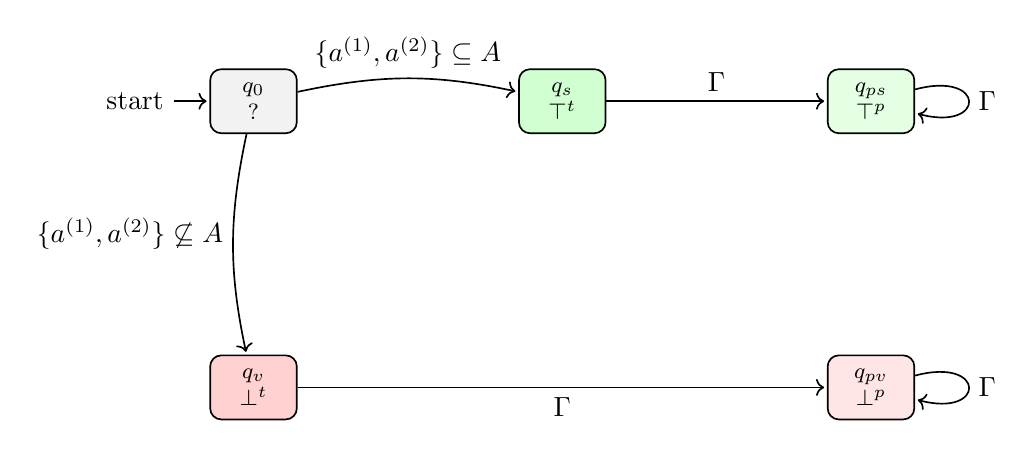
\begin{tikzpicture}[
shorten >=1pt,auto,node distance=28mm,semithick,
  every state/.style={rectangle,rounded corners,draw,minimum width=11mm,
    minimum height=7.5mm,inner sep=5pt,font=\footnotesize,align=center}
]

% --- states ---------------------------------------------------
\node[initial,state,fill=gray!10] (q0)  {$q_0$\\[0.2pt]$\mathsf{?}$};
\node[state,fill=green!18,right=of q0] (qs)  {$q_s$\\[0.2pt]$\topt$};
\node[state,fill=red!18,below=of q0]   (qv)  {$q_v$\\[0.2pt]$\bott$};
\node[state,fill=green!10,right=of qs] (qps) {$q_{ps}$\\[0.2pt]$\topp$};
\node[state,fill=red!10,below=of qps]  (qpv) {$q_{pv}$\\[0.2pt]$\botp$};

% --- transitions ----------------------------------------------
\path[->]
  (q0) edge[bend left=12] node[above,pos=0.5]
    {$\{a^{(1)},a^{(2)}\}\subseteq A$} (qs)
  (q0) edge[bend right=12] node[left,pos=0.45]
    {$\{a^{(1)},a^{(2)}\} \not\subseteq A$} (qv)
  (qs)  edge node[above] {$\Gamma$} (qps)
  (qv)  edge node[below] {$\Gamma$} (qpv)
  (qps) edge[loop right] node {$\Gamma$} (qps)
  (qpv) edge[loop right] node {$\Gamma$} (qpv);
\end{tikzpicture}
\caption{Compact 5-verdict Moore machine for the obligation literal
$\obl[1]{a}$. 
Each node displays its internal state and the corresponding output verdict $\in\tightverdicts$.
The first joint execution of $a^{(1)}$ and $a^{(2)}$ yields~$\topt$,
otherwise~$\bott$; subsequent steps emit the post-frontier verdicts
$\topp$ or $\botp$.}
\label{fig:moore-obligation-compact}
\end{figure}


\subsubsection*{Construction for Binary Contract Operators}

For binary contract operators of the form $C\ \textsf{op}\ C'$ with
$\textsf{op} \in \{\wedge,\ ;\ ,\ \repair\}$, the monitor for the composite contract is obtained by combining the already constructed monitors
$\tsmc(C)$ and $\tsmc(C')$. Each operator has its own monitor construction,
defined below for conjunction, sequence, and reparation. We begin with the
conjunction case.


\begin{definition}[Tight Satisfaction Monitor Construction for Conjunction]
\label{def:moore-5-conj}
Let $C$ and $C'$ be contracts in \cDL, and let
\[
\tsmc(C)  = (Q, q_0, \Gamma, \tightverdicts, \delta, \lambda_5)
\quad\text{and}\quad
\tsmc(C') = (Q', q'_0, \Gamma, \tightverdicts, \delta', \lambda'_5).
\]
The tight satisfaction monitor construction for the conjunction
$C \wedge C'$, written $\tsmc_{\wedge}(C,C')$, is defined as:
\[
\tsmc_{\wedge}(C,C')
  = (Q_{\wedge}, q_0^{\wedge}, \Gamma, \tightverdicts, \delta_{\wedge}, \lambda_5^{\wedge}).
\]

\begin{itemize}
  \item The state set is the Cartesian product
  \[
    Q_{\wedge} = Q \times Q',
  \]
  with the initial state
  \[
    q_0^{\wedge} = (q_0,\,q'_0).
  \]

  \item The output function is
  \[
    \lambda_5^{\wedge}(x,y) =
    \lambda_{5}^{\textsf{comb}}\!\big(\lambda_5(x),\ \lambda'_5(y)\big),
  \]
  where $\lambda_{5}^{\textsf{comb}}$ is the conjunction-combination table:
  \[
  \begin{array}{c|ccccc}
  \lambda_{5}^{\textsf{comb}}(v_1,v_2) & \mathsf{?} & \topt & \bott & \topp & \botp\\\hline
  \mathsf{?} & \mathsf{?} & \mathsf{?} & \bott & \mathsf{?} & \botp\\
  \topt      & \mathsf{?} & \topt      & \bott & \topt      & \botp\\
  \bott      & \bott      & \bott      & \bott & \bott      & \botp\\
  \topp      & \mathsf{?} & \topt      & \bott & \topp      & \botp\\
  \botp      & \botp      & \botp      & \botp & \botp      & \botp
  \end{array}
  \]

  \item The transition function is the synchronous product:
  \[
    \delta_{\wedge}\big((x,y),A\big)
      = \big(\delta(x,A),\ \delta'(y,A)\big),
  \]
  for all $(x,y)\in Q_{\wedge}$ and $A\in\Gamma$.
\end{itemize}
\end{definition}


\noindent
\textbf{Partial dominance rules for $\wedge$.}
The monitor for $C \wedge C'$ checks both components at the same time and decides the global verdict according to the following rules:

\begin{itemize}
  \item If any component gives $\botp$, the result is $\botp$:
  \[
  \forall v\in\tightverdicts:\quad \botp \sqcap v = \botp,
  \]
  That is, once a permanent violation appears, the whole conjunction is permanently violated.
  \item If any component gives $\bott$, and none is permanent, the result is $\bott$:
  \[
  \forall v\in\{\mathsf{?},\topt,\topp\}:\quad \bott \sqcap v = \bott,
  \]
  That is, a single tight violation makes the conjunction fail tightly.
  \item Tight and permanent success combine as the weakest success:
  \[
  \topt \sqcap \topt = \topt,\qquad
  \topt \sqcap \topp = \topt,\qquad
  \topp \sqcap \topp = \topp,
  \]
  The conjunction is only permanently satisfied when both parts are permanent.
  \emph{Note:} The case $\topt \sqcap \topp = \topt$ reflects that if one component is exactly at its satisfaction frontier ($\topt$) while the other is already past it ($\topp$), the conjunction as a whole is determined by the later of the two, effectively placing the global frontier at the current step.
  \item If both sides are undecided or only partly satisfied, the result stays $\mathsf{?}$:
  \[
  \mathsf{?}\sqcap v = \mathsf{?}\quad\text{for }v\in\{\mathsf{?},\topt,\topp\},
  \]
  The monitor waits until a clear outcome appears.
  \item The operator is symmetric:
  \[
  v_1\sqcap v_2 = v_2\sqcap v_1,
  \]
  The order of operands does not matter.
\end{itemize}


\begin{lemma}[Correctness of the conjunctive monitor construction]
\label{lem:conj-correct}
Let 
\[
\tsmc(C)  = (Q, q_0, \Gamma, \tightverdicts, \delta, \lambda_5)
\quad\text{and}\quad
\tsmc(C') = (Q', q'_0, \Gamma, \tightverdicts, \delta', \lambda'_5)
\]
and let
\[
\tsmc(C \wedge C')
  = (Q_{\wedge}, q_0^{\wedge}, \Gamma, \tightverdicts, \delta_{\wedge}, \lambda_5^{\wedge})
\]
be the conjunction monitor defined in Definition~\ref{def:moore-5-conj}.
For every trace $\pi$, the output of the conjunction monitor satisfies:
\[
\lambda_5^{\wedge}(\delta_\wedge(q_0^\wedge,\pi))=
\semfive{\pi \vDash C \wedge C'}.\]
\end{lemma}

\noindent
\textbf{Proof sketch.}
The monitor $\tsmc_{\wedge}(\tsmc(C),\tsmc(C'))$ runs both component monitors in parallel and
computes its output using the conjunction-combination table
$\lambda_{5}^{\textsf{comb}}$. The correctness follows from the prefix-based
tight semantics of $C \wedge C'$.

\begin{itemize}
  \item Permanent violation in either component produces $\botp$ immediately.
  \item A tight violation in one component produces $\bott$ whenever no permanent result is already present.
  \item Satisfaction requires both components to reach satisfaction states.  
        If one is in $\topp$ or $\topt$ and the other is non-violating, the
        combined verdict matches the corresponding entry in the table.
  \item If both components remain undecided, the output is $\mathsf{?}$.
\end{itemize}

These cases match exactly the clauses for tight satisfaction, tight violation,
post-satisfaction, and post-violation for the contract $C \wedge C'$. The monitor, therefore, correctly implements the tight semantics of conjunction.
\qed


Sequential composition is the second binary operator of \cDL. Given two already
constructed monitors $\tsmc(C)$ and $\tsmc(C')$, the monitor for the composite
contract $C\,;\,C'$ must first execute $C$ on the incoming trace and, once $C$
reaches tight satisfaction, must continue execution with $C'$ on the remaining
suffix. The construction below reuses the state spaces of both components by redirecting transitions that correspond to the tight success of $C$
into the initial state of $C'$. This yields a tight prefix monitor that exactly matches the semantics of sequential composition.

\begin{definition}[Sequential Monitor Construction]
\label{def:moore-seq}
Let
\[
\tsmc(C)  = (Q, q_0, \Gamma, \tightverdicts, \delta, \lambda_5)
\quad\text{and}\quad
\tsmc(C') = (Q', q'_0, \Gamma, \tightverdicts, \delta', \lambda'_5)
\]
be the tight satisfaction monitors of $C$ and $C'$.  
The tight satisfaction monitor for the sequential composition
$C\,;\,C'$, written $\tsmc_{\bm{;}}(C,C')$, is defined as:
\[
\tsmc_{\bm{;}}(\tsmc(C),\tsmc(C'))
  = (Q_{;}, q_0^{;}, \Gamma, \tightverdicts, \delta_{;}, \lambda_5^{;}).
\]

\begin{itemize}
  \item The state set is
  \[
    Q_{;} = (Q \setminus Q^{+})\ \cup\ Q',
  \]
  where
  \[
    Q^{+} = \{\,x \in Q \mid \lambda_5(x) \in \{\topt,\topp\}\,\},
  \]
  and the initial state is
  \[
    q_0^{;} = q_0.
  \]

  \item The transition function is
  \[
  \delta_{;}(q,A) =
  \begin{cases}
    q'_0 
      & \text{if } q\in Q \text{ and } \lambda_5(\delta(q,A)) = \topt, \\[4pt]
    \delta(q,A)
      & \text{if } q\in Q \text{ and } \lambda_5(\delta(q,A)) \notin \{\topt,\topp\}, \\[4pt]
    \delta'(q,A)
      & \text{if } q\in Q'. \\
  \end{cases}
  \]

  \item The output function is
  \[
  \lambda_5^{;}(x) =
  \begin{cases}
    \lambda_5(x)  & \text{if } x\in Q,\\
    \lambda'_5(x) & \text{if } x\in Q'. \\
  \end{cases}
  \]
\end{itemize}
\end{definition}

\noindent
\textbf{Intuition.}
The construction implements the idea that $C$ must succeed tightly before
$C'$ becomes active. All states of $C$ that already correspond to tight
satisfaction ($\lambda_5(x)=\topt$ or $\topp$) are removed, since execution
should never continue inside them. Any transition in $C$ that would have
entered such a removed state is redirected to the initial state $q'_0$ of
$C'$, thereby starting the second contract at the exact prefix where $C$
achieves tight success. All other transitions behave exactly as in the
original monitors. The resulting machine therefore behaves as $C$ until $C$
succeeds tightly, after which it behaves as $C'$ for the remainder of the
trace.

\begin{lemma}[Correctness of the sequential monitor construction]
\label{lem:seq-correct}
Let $\tsmc(C)$ and $\tsmc(C')$ be the monitors for $C$ and $C'$,
and let $\tsmc_{\bm{;}}(\tsmc(C),\tsmc(C'))
= (Q_{;}, q_0^{;}, \Gamma, \tightverdicts, \delta_{;}, \lambda_5^{;})$. For every trace $\pi$, the monitor outputs the same verdict according to the sequence semantics:
\[
\lambda_5^{;}\big(\delta_{;}(q_0^{;},\pi)\big)=
\semfive{\pi \vDash C;C'}.
\]
\end{lemma}
\textbf{Proof.}
The proof is by induction on the length of the input trace $\pi$.

    \begin{proof}
        Let $M:=\tsmc_{\bm{;}}(\tsmc(C),\tsmc(C'))=(Q_{;}, q_0^{;}, \Gamma, \tightverdicts, \delta_{;}, \lambda_5^{;})$.
        We prove by induction on $n:=|\pi|$ that
        \[
        \lambda_5^{;}\big(\delta_{;}(q_0^{;},\pi)\big)
        \;=\;
        \semfive{\pi \vDash C;C'}.
        \]
        
        \paragraph{Base case ($n=0$).}
        For $\pi=\emptytrace$ we have $\delta_{;}(q_0^{;},\emptytrace)=q_0$ and thus
        \[
        \lambda_5^{;}\big(\delta_{;}(q_0^{;},\emptytrace)\big)=\lambda_5(q_0)=\mathsf{?}.
        \]
        This matches the tight semantics of $C;C'$ on the empty trace: no decisive prefix for $C$ has been reached and $C'$ cannot be active yet.
        
        \paragraph{Inductive step.}
        Assume the claim holds for all traces of length $n$.
        Let $\pi$ be a trace of length $n{+}1$ and write $\pi=\pi'\concat\trace{A}$ with $|\pi'|=n$ and $A\in\Gamma$.
        Let $s:=\delta_{;}(q_0^{;},\pi')$ be the state reached after reading $\pi'$.
        We distinguish whether the monitor is already executing the right component.
        
        \smallskip
        \noindent\emph{Case 1: $s\in Q'$.}
        Then, by Definition~\ref{def:moore-seq}, $\delta_{;}(s,A)=\delta'(s,A)$ and $\lambda_5^{;}(s)=\lambda'_5(s)$, hence
        \[
        \lambda_5^{;}\big(\delta_{;}(q_0^{;},\pi)\big)
        =
        \lambda'_5\big(\delta'(s,A)\big).
        \]
        Reaching a state of $Q'$ means that the switch from $C$ to $C'$ has already happened at some earlier prefix, and from that point on the sequential monitor behaves exactly as the monitor for $C'$ on the remaining suffix.
        Therefore the tight semantics of $C;C'$ on $\pi$ is determined by the verdict of $C'$ on that suffix.
        By correctness of $\tsmc(C')$ (established for the tight monitor construction),
        the right-hand side equals $\semfive{\pi \vDash C;C'}$.
        
        \smallskip
        \noindent\emph{Case 2: $s\in Q$.}
        Let $t:=\delta(s,A)$ be the next state of the left monitor.
        There are two subcases.
        
        \smallskip
        \noindent\emph{Case 2(a): $\lambda_5(t)=\topt$.}
        Then Definition~\ref{def:moore-seq} redirects the transition to $q'_0$, so $\delta_{;}(s,A)=q'_0$ and
        \[
        \lambda_5^{;}\big(\delta_{;}(q_0^{;},\pi)\big)
        =
        \lambda_5^{;}(q'_0)
        =
        \lambda'_5(q'_0)
        =
        \mathsf{?}.
        \]
        Semantically, this is exactly the step where $C$ reaches its tight satisfaction frontier on the prefix $\pi$, and the contract $C'$ becomes active on the remaining suffix.
        At this switching moment, the suffix is empty, so the status of $C'$ is undecided, and the sequence verdict is $\mathsf{?}$.
        Thus the monitor output matches $\semfive{\pi \vDash C;C'}$.
        
        \smallskip
        \noindent\emph{Case 2(b): $\lambda_5(t)\notin\{\topt,\topp\}$.}
        Then the switch has not occurred, so $\delta_{;}(s,A)=t$ and $\lambda_5^{;}(t)=\lambda_5(t)$.
        Therefore
        \[
        \lambda_5^{;}\big(\delta_{;}(q_0^{;},\pi)\big)
        =
        \lambda_5(t)
        =
        \semfive{\pi \vDash C}.
        \]
        Before $C$ reaches tight satisfaction, the sequence semantics is governed by the left component on the current prefix, hence $\semfive{\pi \vDash C}=\semfive{\pi \vDash C;C'}$ in this case.
        So the equality holds.
        
        All cases agree with the semantic clauses of sequential composition, so the induction closes.
        \end{proof}



\begin{definition}[Reparation Monitor Construction]
\label{def:moore-repair}
Let
\[
\tsmc(C)  = (Q, q_0, \Gamma, \tightverdicts, \delta, \lambda_5)
\quad\text{and}\quad
\tsmc(C') = (Q', q'_0, \Gamma, \tightverdicts, \delta', \lambda'_5)
\]
be the tight satisfaction monitors for $C$ and $C'$.  
The monitor for the reparation contract $C\repair C'$, written
\[
\tsmc_{\repair}(C,C'),
\]
is defined as the tuple
\[
\tsmc_{\repair}(\tsmc(C),\tsmc(C'))
  = (Q_{\repair}, q_0^{\repair}, \Gamma, \tightverdicts, \delta_{\repair}, \lambda_5^{\repair}).
\]

\begin{itemize}
  \item The state set is
  \[
    Q_{\repair} = (Q \setminus Q^{-})\ \cup\ Q',
  \]
  where
  \[
    Q^{-} = \{\,q \in Q \mid \lambda_5(q) \in \{\bott,\botp\}\,\},
  \]
  and the initial state is
  \[
    q_0^{\repair} = q_0.
  \]

  \item The transition function is
  \[
    \delta_{\repair}(q,A)=
    \begin{cases}
      q'_0
        & \text{if } q\in Q \text{ and } \lambda_5(\delta(q,A))=\bott,\\[4pt]
      \delta(q,A)
        & \text{if } q\in Q \text{ and } \lambda_5(\delta(q,A))\notin\{\bott,\botp\},\\[4pt]
      \delta'(q,A)
        & \text{if } q\in Q'.\\
    \end{cases}
  \]

  \item The output function is
  \[
     \lambda_5^{\repair}(q)=
     \begin{cases}
       \lambda_5(q)   & \text{if } q\in Q,\\[2pt]
       \lambda'_5(q)  & \text{if } q\in Q'.\\
     \end{cases}
  \]
\end{itemize}
\end{definition}


\noindent
\textbf{Intuition.}
The reparation operator activates the secondary contract $C'$ after the primary contract $C$ reaches a tight failure. The construction mirrors the sequential case, except that the redirection applies to transitions leading to a tight violation of $C$ rather than to those leading to tight satisfaction.

All states of $C$ whose verdicts are already violating
($\lambda_5(q)\in\{\bott,\botp\}$) are removed. Every transition in $C$ that
would enter such a state is redirected to $q'_0$, the initial state of $C'$.
This starts $C'$ exactly at the tight prefix where $C$ tightly fails.  

As long as no violation occurs, the monitor behaves exactly as $C$. Once a tight failure is detected, the remaining input is processed by $C'$.

\begin{lemma}[Correctness of the reparation monitor construction]
\label{lem:rep-correct}
Let $\tsmc(C)$ and $\tsmc(C')$ be the monitors for $C$ and $C'$, and let
\[
\tsmc_{\repair}(\tsmc(C),\tsmc(C'))
  = (Q_{\repair}, q_0^{\repair}, \Gamma, \tightverdicts, \delta_{\repair}, \lambda_5^{\repair})
\]
be the monitor constructed in Definition~\ref{def:moore-repair}.
Then, for every trace $\pi$, the monitor outputs the right verdict as specified by the tight semantics:
\[
\lambda_5^{\repair}(\delta_{\repair}(q_0^{\repair},\pi)) = \semfive{\pi \vDash C \repair C'}.
\]
\end{lemma}
\begin{proof}[Proof sketch]
The argument follows exactly the same scheme as the proof of
Lemma~\ref{lem:seq-correct} for sequential composition.

The reparation monitor behaves as the tight monitor for $C$ as long as no tight violation occurs.
By the correctness invariant of $\tsmc(C)$, all prefixes before the first tight violation are evaluated exactly as prescribed by the tight semantics of $C\repair C'$.

At the unique prefix where $C$ reaches a tight violation ($\bott$), the construction redirects the transition to the initial state $q'_0$ of the monitor for $C'$.
This corresponds precisely to the semantic clause that activates the reparation contract after the first decisive failure of $C$.

From that point on, the monitor evolves exactly as $\tsmc(C')$ on the remaining suffix.
By the inductive correctness of the tight monitor construction for $C'$, the emitted verdict coincides with the tight semantics of $C'$ on that suffix.

Since all other transitions are unchanged and no ambiguity about the switching point is possible, the monitor output agrees with the tight semantics of $C\repair C'$ on all finite traces.
\end{proof}






\begin{remark}[Relation to Control Phases and Prior Work]
  \label{rem:control-phases}
  The structural constructions in Definitions~\ref{def:moore-seq} and~\ref{def:moore-repair} serve as the static counterpart to the \emph{control-phase} view described in runtime verification frameworks such as \cite{falcone2009runtime,bartocci2018rv}.
  While these standard frameworks often rely on an explicit control variable $m \in \{\mathbf{L}, \mathbf{R}\}$ to dynamically track whether the left ($\mathbf{L}$) or right ($\mathbf{R}$) component is active, our transformation embeds this logic directly into the transition graph.
  We achieve this by eliminating the terminal states of the left monitor and redirecting the decisive transitions—$\topt$ for sequence and $\bott$ for reparation—to the initial state of the right monitor.
  Consequently, this compile-time structure effectively encodes the operational behavior of a mode-augmented monitor that switches phases only when specific conditions are met.
  This design parallels the phase-based semantics where control modes synchronize sub-monitors for sequential patterns like ``\emph{after $C$ succeeds, check $C'$}''.
  Similarly, our reparation composition aligns with the ``\emph{compensatory phase}'' discussed in \cite{governatori2006formal}, where a secondary clause activates only after the primary obligation fails.
  Thus, our constructions realize these phase shifts ($\mathbf{L} \to \mathbf{R}$) at the automaton level, eliminating the need for the explicit control variables used in prior work.
  \end{remark}



\begin{example}[5-Output Moore Monitors for $C_3$ and $C_2 \wedge C_3$]
\label{ex:moore-c3-literals}
The reparation contract $C_3=\obl[1]{\PAY}\repair\obl[1]{\PAYF}$ combines two obligations:
the primary duty $\obl[1]{\PAY}$ to pay rent,
and the secondary reparation $\obl[1]{\PAYF}$ to pay a late fee if the first is violated.
In addition, $C_2=\perm[1]{\OCC}$ grants the tenant (agent~2) permission to occupy the property.
Below, we show the literal monitors, their reparation composition, and the conjunction $C_2\wedge C_3$,
with verdict outputs $\tightverdicts=\{\mathsf{?},\topt,\bott,\topp,\botp\}$.


We construct $C_2 \wedge C_3$ by the synchronous product of the 5-output monitors for $C_2=\perm[2]{\OCC}$ and $C_3=\obl[1]{\PAY}\repair\obl[1]{\PAYF}$, then keep only
reachable states and minimize construction~\ref{fig:moore-c3-literals}.
The Letter classes used on edges correspond to  shorthand for literal satisfaction or violation conditions:
\[
\begin{aligned}
\PAY^\surd   &:= \{\,A\in\Gamma \mid \{\PAY^{(1)},\PAY^{(2)}\}\subseteq A\,\}, 
&\qquad \PAY^\times   &:= \Gamma\setminus \PAY^\surd,\\[2pt]
\PAYF^\surd  &:= \{\,A\in\Gamma \mid \{\PAYF^{(1)},\PAYF^{(2)}\}\subseteq A\,\},
&\qquad \PAYF^\times  &:= \Gamma\setminus \PAYF^\surd,\\[2pt]
\OCC^{\surd} &:= \{\,A\in\Gamma \mid \OCC^{(2)}\in A \Rightarrow \OCC^{(1)}\in A\,\},
&\qquad \OCC^{\times} &:= \Gamma\setminus \OCC^{\surd}.
\end{aligned}
\]
Outputs follow the conjunction rule $\Lambda$:
$\bott$ if any conjunct tightly rejects, $\botp$ if any conjunct is post-reject,
$\topt$ when one conjunct hits $\topt$ while the other is already at/past acceptance
($\topt$ or $\topp$), $\topp$ if both are post-accept, and $\mathsf{?}$ otherwise.

Reading Subfigure~\ref{fig:c2andc3} with the letter classes defined above: from $s_0$ (pre) there are three behaviors:
(i) If \,$\OCC^\surd \land \PAY^\surd$\ holds in the current letter, both conjuncts succeed (perm is respected, and the primary obligation is met), so the product emits $\topt$
and moves to post-accept $\topp$.
(ii) If \,$\OCC^{\times}$\ holds, the permission conjunct fails tightly, so the product
emits $\bott$ and then $\botp$ forever.
(iii) If \,$\OCC^\surd \land \PAY^{\times}$\ holds, the reparation branch of $C_3$
is activated, and we move to the waiting state $s_1$ (still $\mathsf{?}$). From $s_1$,
\,$\PAYF^\surd$\ discharges the reparation and triggers $\topt$; otherwise
\,$\PAYF^{\times}$\ yields $\bott$. After $\topt$ (accepting frontier), all continuations
are in $\topp$; after $\bott$ (reject frontier) all continuations are in $\botp$.
Thus, the decisive index for the conjunction is the latter of the two successes when both succeed, or the earlier tight failure when any conjunct fails, exactly as the figure shows.



\begin{figure*}[h!]
\centering
\captionsetup[subfigure]{justification=centering}

% ================================================================
% (a)+(b) side-by-side literal monitors
% ================================================================
\begin{subfigure}[t]{0.48\textwidth}
\centering
\scalebox{0.82}{
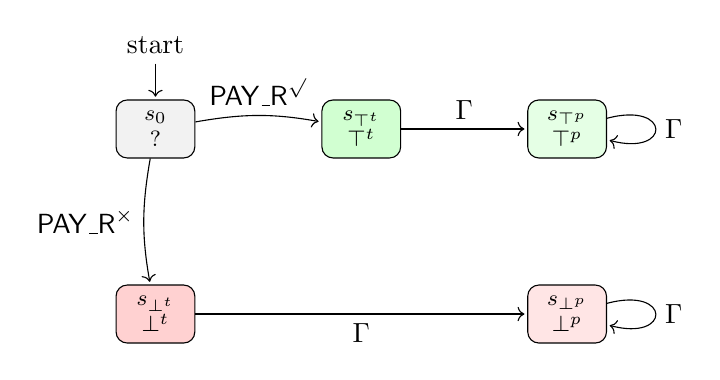
\begin{tikzpicture}[
  ->,shorten >=1pt, node distance=16mm,
  every state/.style={rectangle,rounded corners,draw,minimum width=10mm,
                      minimum height=6mm,inner sep=4pt,font=\footnotesize,align=center}
]
\node[initial, initial where=above,state,fill=gray!10] (q0) {$s_0$\\$\mathsf{?}$};
\node[state,fill=green!18,right=of q0] (qs) {$s_{\topt}$\\$\topt$};
\node[state,fill=red!18,below=of q0] (qv) {$s_{\bott}$\\$\bott$};
\node[state,fill=green!10,right=of qs] (qps) {$s_{\topp}$\\$\topp$};
\node[state,fill=red!10,below=of qps] (qpv) {$s_{\botp}$\\$\botp$};

\path[->]
  (q0) edge[bend left=10] node[above,pos=0.5] {$\PAY^\surd$} (qs)
  (q0) edge[bend right=10] node[left,pos=0.5] {$ \PAY^\times$} (qv)
  (qs) edge node[above] {$\Gamma$} (qps)
  (qv) edge node[below] {$\Gamma$} (qpv)
  (qps) edge[loop right] node {$\Gamma$} ()
  (qpv) edge[loop right] node {$\Gamma$} ();
\end{tikzpicture}}
\caption{$\tsmc_\ell (\obl[1]{\PAY})$
Satisfaction occurs when both agents perform $\PAY$.}
\label{fig:obl-pay}
\end{subfigure}
\hfill
\begin{subfigure}[t]{0.48\textwidth}
\centering
\scalebox{0.82}{
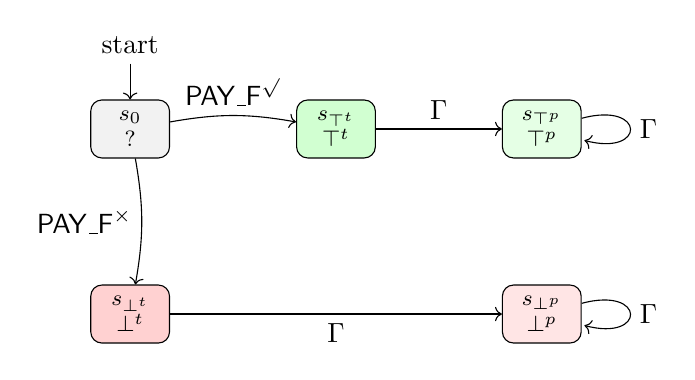
\begin{tikzpicture}[
  ->, node distance=16mm,
  every state/.style={rectangle,rounded corners,draw,minimum width=10mm,
                      minimum height=6mm,inner sep=4pt,font=\footnotesize,align=center}
]
\node[initial,initial where=above,state,fill=gray!10] (q0) {$s_0$\\$\mathsf{?}$};
\node[state,fill=green!18,right=of q0] (qs) {$s_{\topt}$\\$\topt$};
\node[state,fill=red!18,below=of q0] (qv) {$s_{\bott}$\\$\bott$};
\node[state,fill=green!10,right=of qs] (qps) {$s_{\topp}$\\$\topp$};
\node[state,fill=red!10,below=of qps] (qpv) {$s_{\botp}$\\$\botp$};

\path[->]
  (q0) edge[bend left=10] node[above,pos=0.5] {$\PAYF^\surd$} (qs)
  (q0) edge[bend left=10] node[left,pos=0.5] {$\PAYF^\times$} (qv)
  (qs) edge node[above] {$\Gamma$} (qps)
  (qv) edge node[below] {$\Gamma$} (qpv)
  (qps) edge[loop right] node {$\Gamma$} ()
  (qpv) edge[loop right] node {$\Gamma$} ();
\end{tikzpicture}}
\caption{$\tsmc_\ell (\obl[1]{\PAYF})$
Satisfaction occurs when both agents perform $\PAYF$.}
\label{fig:obl-payf}
\end{subfigure}

\vspace{2mm}

% ================================================================
% (c) Reparation composition
% ================================================================
\begin{subfigure}[t]{0.9\textwidth}
\centering
\scalebox{0.9}{
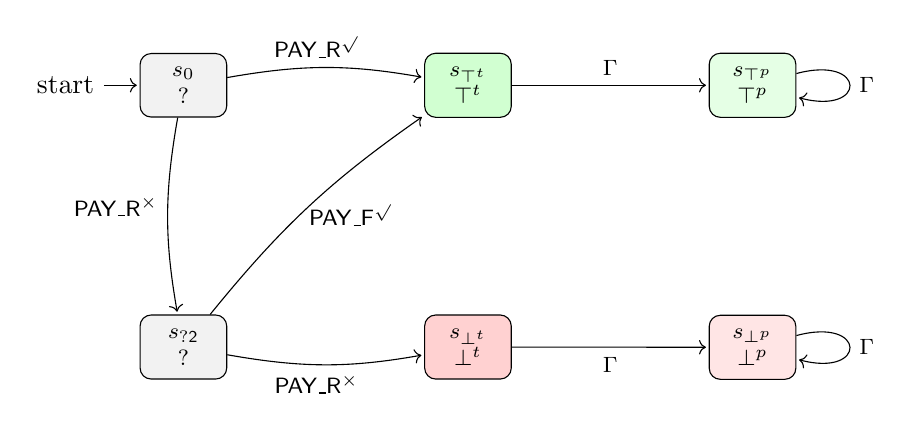
\begin{tikzpicture}[
  ->,shorten >=1pt, node distance=25mm,
  every state/.style={
    rectangle,rounded corners,draw,
    minimum width=11mm,minimum height=7mm,
    inner sep=5pt,font=\footnotesize,align=center}
]
\node[initial,state,fill=gray!10] (q0) {$s_0$\\$\mathsf{?}$};
\node[state,fill=gray!10,below=of q0] (qwait) {$s_{\mathsf{?2}}$\\[0.2pt]$\mathsf{?}$};
\node[state,fill=green!18,right=of q0] (qs) {$s_{\topt}$\\[0.2pt]$\topt$};
\node[state,fill=red!18,right=of qwait] (qv) {$s_{\bott}$\\[0.2pt]$\bott$};
\node[state,fill=green!10,right=of qs] (qps) {$s_{\topp}$\\[0.2pt]$\topp$};
\node[state,fill=red!10,below=of qps] (qpv) {$s_{\botp}$\\[0.2pt]$\botp$};

\path[->]
  (q0) edge[bend left=10]  node[above,pos=0.45] {\footnotesize$\PAY^{\surd}$} (qs)
  (q0) edge[bend right=10] node[left,pos=0.45]  {\footnotesize$\PAY^{\times}$} (qwait)
  (qwait) edge[bend left=8] node[right,pos=0.45] {\footnotesize$\PAYF^{\surd}$} (qs)
  (qwait) edge[bend right=10] node[below,pos=0.45] {\footnotesize$\PAY^{\times}$} (qv)
  (qs) edge node[above] {\footnotesize$\Gamma$} (qps)
  (qv) edge node[below] {\footnotesize$\Gamma$} (qpv)
  (qps) edge[loop right] node {\footnotesize$\Gamma$} ()
  (qpv) edge[loop right] node {\footnotesize$\Gamma$} ();
\end{tikzpicture}}
\caption{Reparation composition $\tsmc_\repair (\obl[1]{\PAY},\obl[1]{\PAYF})$.
The monitor activates $\PAYF$ after tight failure of $\PAY$.}
\label{fig:obl-pay-repair}
\end{subfigure}

\vspace{2mm}

% ================================================================
% (d) Conjunctive composition (C2 and C3)
% ================================================================
\begin{subfigure}[t]{0.9\textwidth}
\centering
\scalebox{0.9}{
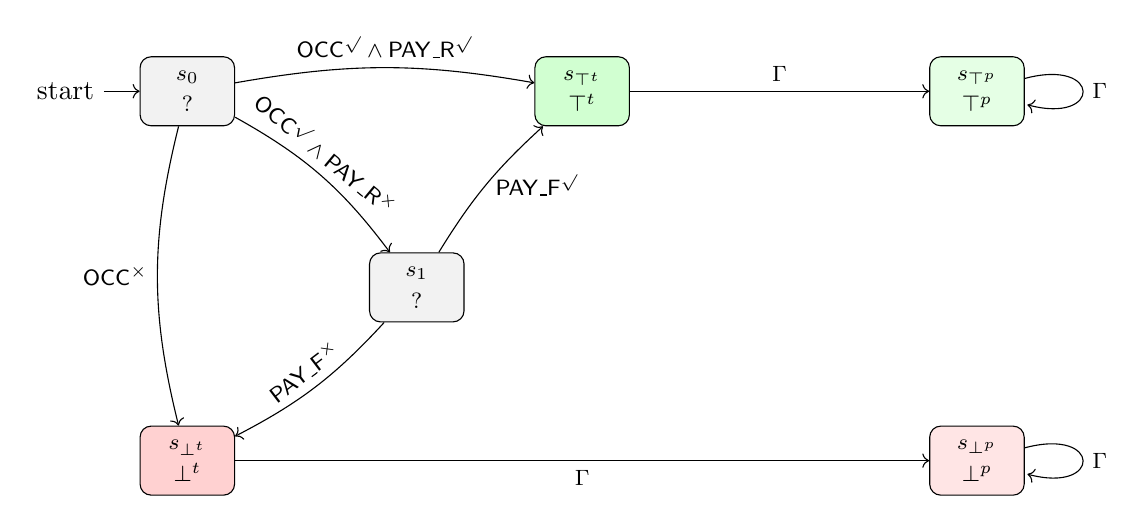
\begin{tikzpicture}[
  ->, node distance=20mm and 18mm,
  every state/.style={
    rectangle,rounded corners,draw,
    minimum width=12mm,minimum height=7mm,
    inner sep=5pt,font=\footnotesize,align=center
  }
]
% States
\node[initial,state,fill=gray!10] (q0) {$s_0$\\[2pt]$\mathsf{?}$};
\node[state, fill=gray!10, below right=16mm and 17mm of q0] (q1) {$s_1$\\[2pt]$\mathsf{?}$};
\node[state,fill=green!18,right=38mm of q0] (qs) {$s_{\topt}$\\[2pt]$\topt$};
\node[state,fill=red!18,below=38mm of q0] (qv) {$s_{\bott}$\\[2pt]$\bott$};
\node[state,fill=green!10,right=38mm of qs] (qps) {$s_{\topp}$\\[2pt]$\topp$};
\node[state,fill=red!10,below=38mm of qps] (qpv) {$s_{\botp}$\\[2pt]$\botp$};

% Transitions
\path[->]
  (q0) edge[bend left=10] node[above,pos=0.5] {\footnotesize$\OCC^\surd \land \PAY^{\surd}$} (qs)
  (q0) edge[bend right=14] node[left,pos=0.5] {\footnotesize$\OCC^{\times}$} (qv)
  (q0) edge[bend left=12] node[pos=0.45,sloped,above] {\footnotesize$\OCC^\surd \land \PAY^{\times}$} (q1)
  (q1) edge[bend left=8] node[right] {\footnotesize$\PAYF^\surd$} (qs)
  (q1) edge[bend left=10] node[sloped,pos=0.5,above] {\footnotesize$\PAYF^{\times}$} (qv)
  (qs) edge node[above] {\footnotesize$\Gamma$} (qps)
  (qv) edge node[below] {\footnotesize$\Gamma$} (qpv)
  (qps) edge[loop right] node {\footnotesize$\Gamma$} ()
  (qpv) edge[loop right] node {\footnotesize$\Gamma$} ();
\end{tikzpicture}}
\caption{Conjunctive composition $\tsmc_{\wedge}(C_2,C_3)$, where $C_2=\perm[1]{\OCC}$.}
\label{fig:c2andc3}
\end{subfigure}


\caption{Literal and composite 5-output Moore monitors for
$C_3=\obl[1]{\PAY}\repair\obl[1]{\PAYF}$.
(a) and (b)~monitors for Literal composing $C_3$  side by side;
(c)~Reparation composition $C_3$;
(d)~Conjunctive composition $C_2 \wedge C_3$,
where $C_2=\perm[1]{\OCC}$ represents the tenant's power to occupy the property. $\OCC^{\surd}:= \{A \mid \{\OCC^{1}\} \not\subset A \sor  \{\OCC^{1},\OCC^{2}\} \subseteq A\}$. 
$\PAY^\surd:= \{A \mid \PAY^{(1)},\PAY^{(2)}\} \subseteq A $. The case $\PAYF^\surd$ is similarly defined as for $\PAY^\surd$.}
\label{fig:moore-c3-literals}
\end{figure*}
\end{example}
\newpage
\subsubsection*{Construction for Binary Regular Expression-Contracts}
Triggered contracts activate their body $C$ once the triggering pattern $re$
reaches its first tight match. Before that point, the monitor behaves exactly as the regular-expression monitor for $re$ and emits only $\mathsf{?}$. Once the trigger fires, the monitor switches permanently to the contract monitor $\tsmc(C)$. If the pattern becomes impossible before it fires, the contract is
vacuously satisfied. The construction follows the same blueprint as sequence and reparation, but applied to the decisive states of the regular expression monitor.

\begin{definition}[Triggered Monitor Construction]
    \label{def:moore-trigger-seq}
    
    \[\text{Let }
    \tsmc(\re)=(Q_r, r_0, \Gamma, \tightverdicts, \delta_r, \lambda_5^r)
    \quad\text{and}\quad
    \tsmc(C)=(Q_c, c_0, \Gamma, \tightverdicts, \delta_c, \lambda_5^c)
    \]
    be five-valued tight satisfaction monitors for the regular expression $\re$ and the contract $C$.
    The triggered monitor for $\trig[re]{C}$ is the machine
    \[
    \tsmc_{\trigg}(\tsmc_{re}(\re),\tsmc(C))
      := (Q_{\trigg}, q_0^{\trigg}, \Gamma, \tightverdicts, \delta_{\trigg}, \lambda_5^{\trigg}).
    \]
    
    \begin{itemize}
      \item The state space includes the open states of the trigger, the states of the contract, and two fresh sink states for vacuous success:
      \[
         Q_{\trigg} := Q_r^{\text{open}} \cup Q_c \cup \{q_{\mathit{vac}}^{\topt}, q_{\mathit{vac}}^{\topp}\},
      \]
      where the reduced regular expressions states are:
      \[
         Q_r^{\text{open}}
         := \{\,q \in Q_r \mid \lambda_5^r(q)\in\{\mathsf{?},\topt,\topp\}\,\}.
      \]
      The initial state is
      \[
        q_0^{\trigg} := r_0.
      \]
    
      \item The transition function $\delta_{\trigg}$ is defined in three parts:
    
      \begin{enumerate}
          \item 
      \textbf{Guard-active region ($q\in Q_r^{\text{open}}$).}
      Let $q'=\delta_r(q,A)$.
      \[
      \delta_{\trigg}(q,A)=
      \begin{cases}
        c_0
          & \text{if } q'\in Q_r^{\topt}
            \quad\text{(first tight match: activate } C\text{)},\\[4pt]
        q_{\mathit{vac}}^{\topt}
          & \text{if } q'\in Q_r^{\bott}
            \quad\text{(trigger impossible: vacuous success)},\\[4pt]
        q'
          & \text{if } q'\in Q_r^{?}
            \quad\text{(guard still open)}.
      \end{cases}
      \]
      
      \item  \textbf{Contract-active region ($y\in Q_c$).} 
      \[
        \delta_{\trigg}(y,A) := \delta_c(y,A).
      \]
      
      \item \textbf{Vacuous success sinks.}
      \[
        \delta_{\trigg}(q_{\mathit{vac}}^{\topt}, A) := q_{\mathit{vac}}^{\topp}, \qquad
        \delta_{\trigg}(q_{\mathit{vac}}^{\topp}, A) := q_{\mathit{vac}}^{\topp}.
      \]
      \end{enumerate}
    
      \item The output function is
      \[
      \lambda_5^{\trigg}(q)=
      \begin{cases}
        \mathsf{?}
          & \text{if } q\in Q_r^{\text{open}},\\[2pt]
        \lambda_5^{c}(q)
          & \text{if } q\in Q_c,\\[2pt]
        \topt
          & \text{if } q = q_{\mathit{vac}}^{\topt},\\[2pt]
        \topp
          & \text{if } q = q_{\mathit{vac}}^{\topp}.
      \end{cases}
      \]
    \end{itemize}
    \end{definition}
    
    
    \paragraph{Intuition.}
    The trigger monitor is obtained with the same redirection recipe used for sequence, but applied to the trigger.
    Keep only states that are still open in the trigger (outputs in \(\{\,\mathsf{?},\topt,\topp\,\}\)). Remove its decisive states.
    Redirect every transition that would be the first tight match of the triggering regular expression (the step that enters \(\topt\)) to the initial state of the contract monitor \(C\).
    From that point on, the global output is exactly the output of \(C\) on the suffix.
    Redirect every transition that would make the trigger impossible (enter \(\bott\) or \(\botp\)) to the fresh vacuous-success sink \(q_{\mathit{vac}}^{\topt}\), which emits \(\topt\) and then permanently \(\topp\).
    While the guard remains open, only the guard component advances and the product emits \(\mathsf{?}\), so no premature verdict appears.
    This realizes the prefix clauses: success either because the trigger never becomes true (vacuous satisfaction), or because it fires at the earliest index (matching the tight prefix) and the suffix satisfies \(C\);
    violation only if the guard fires and the suffix violates \(C\).
    
    \begin{lemma}[Correctness of the triggered monitor construction]
    \label{lem:trigg-correct}
    \[\text{Let } \tsmc_{\trigg}(\tsmc_{re}(\re),\tsmc(C))
          =(Q_{\trigg},\Gamma,\delta_{\trigg},q_0^{\trigg},\lambda_5^{\trigg})\]
    be the monitor constructed in Definition~\ref{def:moore-trigger-seq} for
    $\trig[re]{C}$.
    Then, for every trace $\pi$,
    \[
    \lambda_5^{\trigg}\bigl(\delta_{\trigg}(q_0^{\trigg},\pi)\bigr)
    \;=\;
    \semfive{\pi \vDash \trig[re]{C}}.
    \]
    \end{lemma}
    
    \noindent
    \textbf{Proof sketch.}
    The proof follows the same pattern as for sequence and reparation, by induction on the length of $\pi$.
    
    \smallskip
    \emph{Base case.}
    For $\pi=\emptytrace$ the monitor is in $q_0^{\trigg}=r_0$, the initial state
    of the guard.
    The value
    \[
    \lambda_5^{\trigg}\bigl(\delta_{\trigg}(q_0^{\trigg},\emptytrace)\bigr)
      = \lambda_5^r(r_0) = \mathsf{?}
    \]
    coincides with the tight semantics of $\trig[re]{C}$ on the empty trace: no trigger has fired, and no violation has occurred.
    
    \smallskip
    \emph{Inductive step.}
    Assume the invariant holds for all prefixes of length $n$.
    Consider a prefix
    of length $n{+}1$ and its last letter $A$.
    There are three regions:
    
    \begin{itemize}
      \item \emph{Guard-active region ($x\in Q_r^{\text{open}}$).}
      By construction, $\delta_{\trigg}(x,A)$ is:
      \begin{itemize}
        \item $c_0$, if $\delta_r(x,A)\in Q_r^{\topt}$.
        This is exactly the case
        where $re$ reaches tight success for the first time.
        The next state is the
        initial state of $\tsmc(C)$, so subsequent behavior matches the semantics
        of $C$ on the suffix.
        This realizes the clause “trigger fires at the
        earliest index and the suffix must satisfy $C$”.
        
        \item $q_{\mathit{vac}}^{\topt}$, if $\delta_r(x,A)\in Q_r^{\bott}$, that is, the pattern becomes impossible.
        This state outputs $\topt$ and transitions to the permanent success state $q_{\mathit{vac}}^{\topp}$.
        This matches the semantics where the trigger never fires and $\trig[re]{C}$
        holds vacuously (tight success followed by post-success).
    
        \item $\delta_r(x,A)$ if $\delta_r(x,A)\in Q_r^{?}$, in which case the
        guard remains open, and the global verdict stays $\mathsf{?}$.
        This matches the semantic clause that no decisive information is available as long as neither a match nor an impossibility has been detected.
      \end{itemize}
      The inductive hypothesis on the guard monitor ensures that the moment of redirection coincides with the earliest decisive prefix of $re$.
    
      \item \emph{Contract-active region ($y\in Q_c$).}
      Once the monitor has been redirected into $c_0$, all transitions are given by $\delta_c$, and outputs by $\lambda_5^c$.
      The induction hypothesis for
      $\tsmc(C)$ gives
      \[
      \lambda_5^{\trigg}\bigl(\delta_{\trigg}(q_0^{\trigg},\pi)\bigr)
       = \lambda_5^{c}\bigl(\delta_c(c_0,\pi')\bigr)
       = \semfive{\pi' \vDash C},
      \]
      where $\pi'$ is the suffix after the trigger point.
      This matches the
      semantics of $\trigg[re]{C}$ on all traces where the trigger has fired.
      
      \item \emph{Vacuous success region.}
      If the monitor enters $q_{\mathit{vac}}^{\topt}$ or $q_{\mathit{vac}}^{\topp}$, it correctly emits the success verdicts corresponding to a triggered contract whose trigger can no longer be satisfied.
    \end{itemize}
    
    \smallskip
    \emph{Violation and satisfaction cases.}
    If the trigger fires at some earliest index $k$ and the suffix $\pi^{k+1}$
    violates $C$ tightly or post, the monitor is in the contract-active region and
    outputs the corresponding $\bott$ or $\botp$, which is exactly
    $\semfive{\pi \vDash \trig[re]{C}}$ in this case.
    If the trigger never fires and the guard becomes impossible, the monitor
    outputs $\topt$ and then $\topp$, which matches vacuous satisfaction.
    In all other cases the output remains $\mathsf{?}$, as the semantics of
    $\trigg[re]{C}$ leaves the status undecided.
    
    \smallskip
    \emph{Conclusion.}
    At each prefix, the monitor either simulates the guard with the correct decisive redirection points, simulates $C$ on the correct suffix, or enters the correct vacuous success state.
    Hence
    for every trace $\pi$ the monitor verdict
    \(
    \lambda_5^{\trigg}(\delta_{\trigg}(q_0^{\trigg},\pi))
    \)
    coincides with the five-valued tight semantics of $\trig[re]{C}$.
    \qed





\begin{definition}[Guarded Monitor Construction]
\label{def:moore-guard}
\[\text{Let }
\tsmc(\re)=(Q_r, r_0, \Gamma, \tightverdicts, \delta_r, \lambda_5^r)
\quad\text{and}\quad
\tsmc(C)=(Q_c, c_0, \Gamma, \tightverdicts, \delta_c, \lambda_5^c).
\]
The guarded contract monitor for $\guard[re]{C}$ is the synchronous product
\[
\tsmc_{\guardd}(\tsmc_{re}(\re),\tsmc(C))
  :=(Q_r\times Q_c,\ (r_0,c_0),\ \Gamma,\ \tightverdicts,\ \delta_{\guardd},\ \lambda_5^{\guardd}),
\]
with
\[
\delta_{\guardd}((x,y),A)
  :=(\delta_r(x,A),\delta_c(y,A)).
\]
The output verdict of the guarded monitor is determined by jointly inspecting the current verdicts of the guard and the contract components, according to the following case distinction.
\[
\lambda_5^{\guardd}(x,y)=
\begin{cases}
\bott
  & \text{if }\lambda_5^r(x)\in\{\mathsf{?},\topt,\topp\}
    \ \text{and }\lambda_5^c(y)=\bott,\\[2pt]
\botp
  & \text{if }\lambda_5^r(x)\in\{\mathsf{?},\topt,\topp\}
    \ \text{and }\lambda_5^c(y)=\botp,\\[2pt]
\topt
  & \text{if }\lambda_5^r(x)=\bott
    \ \text{and }\lambda_5^c(y)\in\{\mathsf{?},\topt,\topp\},\\[2pt]
\topp
  & \text{if }\lambda_5^r(x)=\botp
    \ \text{and }\lambda_5^c(y)\in\{\mathsf{?},\topt,\topp\},\\[2pt]
\topt
  & \text{if }\lambda_5^r(x)\in\{\topt,\topp\}
    \ \text{and }\lambda_5^c(y)=\topt,\\[2pt]
\topp
  & \text{if }\lambda_5^r(x)\in\{\topt,\topp\}
    \ \text{and }\lambda_5^c(y)=\topp,\\[2pt]
\mathsf{?}
  & \text{otherwise.}
\end{cases}
\]
\end{definition}



\paragraph{Intuition.}
The guard reads both monitors in lockstep and enforces:

\begin{itemize}
  \item \emph{Open guard.} While the guard is open
  \(\bigl(\lambda_r\in\{\mathsf{?},\topt,\topp\}\bigr)\), i.e. exactly when \(\pi\ \clossat\ re\),
  any tight or post failure of \(C\) becomes the global failure:
  \begin{align*}
    \pi\ \violt\ \guard[re]{C} &\iff (\pi\ \clossat\ re)\ \land\ (\pi\ \violt\ C),\\
    \pi\ \postviol\ \guard[re]{C} &\iff (\pi\ \clossat\ re)\ \land\ (\pi\ \postviol\ C).
  \end{align*}

  \item \emph{Guard impossible.} If the guard becomes impossible
  \(\bigl(\lambda_r\in\{\bott,\botp\}\bigr)\), we accept provided \(C\) has not failed:
  \begin{align*}
    \pi\ \satt\ \guard[re]{C} &\iff (\pi\ \violt\ re)\ \land\ (\pi\ \clossat\ C),\\
    \pi\ \postsat\ \guard[re]{C} &\iff (\pi\ \violt\ re)\ \land\ (\pi\ \postsat\ C).
  \end{align*}

  \item \emph{Guard fired/closed.} When the guard has fired/closed
  \(\bigl(\lambda_r\in\{\topt,\topp\}\bigr)\), we require \(C\) to (tight/post) succeed:
  \begin{align*}
    \pi\ \satt\ \guard[re]{C} &\iff (\pi\ \clossat\ re)\ \land\ (\pi\ \satt\ C),\\
    \pi\ \postsat\ \guard[re]{C} &\iff (\pi\ \clossat\ re)\ \land\ (\pi\ \postsat\ C).
  \end{align*}
\end{itemize}
Note that $\pi\ \clossat\ re$ holds exactly when $\lambda_5^r\in{\mathsf{?},\topt,\topp}$.
The resulting case table is symmetric and total, and it collapses to the expected two-valued clauses once tight/post outcomes are merged into satisfied vs.\ violated.

\begin{lemma}[Correctness of the guarded monitor construction]
\label{lem:guard-correct}
\[\text{Let }
\tsmc_{\guardd}(\tsmc_{re}(\re),\tsmc(C))
  =(Q_{\guardd},q_0^{\guardd},\Gamma,\tightverdicts,\delta_{\guardd},\lambda_5^{\guardd})
\]
be the monitor constructed in Definition~\ref{def:moore-guard} for
$\guard[re]{C}$.  
Then, for every finite trace $\pi$,
\[
\lambda_5^{\guardd}\bigl(\delta_{\guardd}(q_0^{\guardd},\pi)\bigr)
  \;=\;
\semfive{\pi \vDash \guard[re]{C}}.
\]
\end{lemma}
\noindent\textbf{Proof sketch.}
The argument proceeds by induction on the length of $\pi$.  
The guarded monitor is a synchronous product of $\tsmc(re)$ and $\tsmc(C)$,
with the output governed by the case distinction in
Definition~\ref{def:moore-guard}.  
Each region of the case table matches exactly one of the semantic clauses for 
$\guard[re]{C}$.

\smallskip
\emph{Base case.}
For $\pi=\emptytrace$ we have
\[
\lambda_5^{\guardd}\bigl(\delta_{\guardd}(q_0^{\guardd},\emptytrace)\bigr)
  = \lambda_5^{\guardd}(r_0,c_0),
\]
which yields $\mathsf{?}$ in agreement with
$\semfive{\emptytrace \vDash \guard[re]{C}}$.

\smallskip
\emph{Inductive step.}
Assume correctness for all prefixes of length $n$.
Consider $\pi[n{+}1]$ with last letter $A$ and let
\[
(x',y') := \delta_{\guardd}((x,y),A)
           = (\delta_r(x,A),\delta_c(y,A)).
\]

There are three semantic regions, corresponding to the three guard statuses.

\begin{itemize}
  \item \textbf{Guard open}
  \(\lambda_5^r(x)\in\{\mathsf{?},\topt,\topp\}\).  
  This means $\pi$ still possibly satisfies the guard.  
  The guarded semantics requires that any tight or post failure of $C$ becomes the global failure.  
  The monitor table assigns $\bott$ or $\botp$ precisely in these cases, and
  $\mathsf{?}$ otherwise, matching
  \[
  \semfive{\pi \vDash \guard[re]{C}}
    = \semfive{\pi \vDash C}
    \quad\text{as long as $re$ is still open.}
  \]

  \item \textbf{Guard impossible}
  \(\lambda_5^r(x)\in\{\bott,\botp\}\).  
  This corresponds exactly to $\pi\ \violt\ re$.  
  The guarded semantics declares vacuous acceptance provided that $C$ has not already failed.  
  The output table assigns $\topt$ or $\topp$ if $C$ has not failed, and
  propagates $\bott$ or $\botp$ if it has.  
  This matches the semantic requirements for vacuous satisfaction.

  \item \textbf{Guard closed (triggered or concluded)}
  \(\lambda_5^r(x)\in\{\topt,\topp\}\).  
  In this region, the guard has fired or completed successfully, and the
  semantics require $C$ to satisfy or to fail.  
  The output table combines the post-accept and tight-accept verdicts of $C$
  with those of $re$ exactly as demanded by the five-valued semantics:
  \[
     \semfive{\pi \vDash \guard[re]{C}}
       = \semfive{\pi \vDash C}
       \quad\text{once $re$ has closed.}
  \]
\end{itemize}

\smallskip
\emph{Conclusion.}
At each prefix of $\pi$, the guarded monitor outputs exactly the verdict
prescribed by the five-valued semantics of $\guard[re]{C}$.  
Thus
\[
\lambda_5^{\guardd}\bigl(\delta_{\guardd}(q_0^{\guardd},\pi)\bigr)
  = \semfive{\pi \vDash \guard[re]{C}}
\]
for all traces $\pi$.
\qed







\subsubsection*{Construction for repetition contracts}

Repetition contracts describe behaviors that must be satisfied several times in
sequence. The monitor construction follows the intuition that each repetition runs an independent copy of the monitor for $C$, with the next copy becoming active exactly when the previous one reaches tight success. For finite
repetition $C^n$, this results in $n$ chained monitors. For unbounded
repetition $\repit{C}$, we obtain an infinite cycle without ever reporting
tight success.

\medskip
The following constructions make these ideas explicit.
\begin{definition}[Tight monitor construction for finite repetition $\tsmc_\nrep(n,C)$]
\label{def:moore-repeat-finite}
\[\text{Let } \tsmc(C)=(Q,q_0,\Gamma,\tightverdicts,\delta,\lambda_5)\]
be the five-valued tight satisfaction monitor for $C$.  
For $n\in\mathbb{N}^*$, the tight monitor for the finite repetition contract
$\tsmc_\nrep(n,C)$ is defined as
\[
\tsmc_{\nrep}(n,C)
  := (Q_{\nrep},q_0^{\nrep},\Gamma,\tightverdicts,\delta_{\nrep},\lambda_5^{\nrep}).
\]

\medskip
\noindent\emph{Disjoint copies.}
For each $i\in\{1,\dots,n\}$, create a disjoint copy of the base monitor:
\[
Q^{(i)}=\{q^{(i)}\mid q\in Q\},\qquad
\delta^{(i)}(q^{(i)},A)=(\delta(q,A))^{(i)},\qquad
\lambda_5^{(i)}(q^{(i)})=\lambda_5(q).
\]
Write $q_0^{(i)}$ for the copy of $q_0$.

\medskip
\noindent\emph{State space and start state.}
\[
Q_{\nrep}
  := \Bigl(\bigcup_{i=1}^n Q^{(i)}\Bigr)\cup\{q_{\topp},q_{\botp}\},
\qquad
q_0^{\nrep} := q_0^{(1)},
\]
where $q_{\topp}$ and $q_{\botp}$ are fresh post-success and post-failure sinks.

\medskip
\noindent\emph{Transition function.}  
For $1\le i\le n-1$:
\[
\delta_{\nrep}(q^{(i)},A)=
\begin{cases}
q_0^{(i+1)}
   & \text{if }\lambda_5^{(i)}(\delta^{(i)}(q^{(i)},A))=\topt,\\[2pt]
\delta^{(i)}(q^{(i)},A)
   & \text{if }\lambda_5^{(i)}(\delta^{(i)}(q^{(i)},A))
      \notin\{\topt,\topp\}.
\end{cases}
\]
For the last copy $i=n$:
\[
\delta_{\nrep}(q^{(n)},A)=
\begin{cases}
q_{\topp}
   & \text{if }\lambda_5^{(n)}(\delta^{(n)}(q^{(n)},A))=\topt,\\[2pt]
\delta^{(n)}(q^{(n)},A)
   & \text{if }\lambda_5^{(n)}(\delta^{(n)}(q^{(n)},A))
      \notin\{\topt,\topp\}.
\end{cases}
\]
Sink states absorb:
\[
\delta_{\nrep}(q_{\topp},A)=q_{\topp},
\qquad
\delta_{\nrep}(q_{\botp},A)=q_{\botp}.
\]

\medskip
\noindent\emph{Output function.}
For $q^{(i)}\in Q^{(i)}$:
\[
\lambda_5^{\nrep}(q^{(i)})=
\begin{cases}
\bott & \text{if }\lambda_5^{(i)}(q^{(i)})=\bott,\\
\mathsf{?} & \text{if }\lambda_5^{(i)}(q^{(i)})
            \in\{\mathsf{?},\topt,\topp\}.
\end{cases}
\]
For sink states:
\[
\lambda_5^{\nrep}(q_{\topp})=\topp,
\qquad
\lambda_5^{\nrep}(q_{\botp})=\botp.
\]

\medskip
\noindent
This completes the construction of the five-valued monitor for $C^n$.
\end{definition}

\begin{lemma}[Correctness of the finite repetition monitor]
\label{lem:repeat-finite-correct}
For every finite trace $\pi$, contract $C$, and
$\tsmc_{\nrep}(n,C)
  := (Q_{\nrep},q_0^{\nrep},\Gamma,\tightverdicts,\delta_{\nrep},\lambda_5^{\nrep})$, the following holds
\[
\lambda_5^{\nrep}\bigl(\delta_{\nrep}(q_0^{\nrep},\pi)\bigr)
   = \semfive{\pi \vDash C^n}.
\]
\end{lemma}




In the next sections, we use the definitions of the different languages in the semantics of \cdl, along with automata constructions and transformations, to enable automatic detection of violations and the attribution of blame for synchronous interactions over contracts in \cDL.


\begin{definition}[Tight monitor construction for unbounded repetition $\repit{C}$]
\label{def:moore-repeat-unbounded}
Let
\[
\tsmc(C)=(Q,q_0,\Gamma,\tightverdicts,\delta,\lambda_5)
\]
be the tight satisfaction monitor for $C$.
The monitor for the unbounded repetition $\repit{C}$ is defined as
\[
\tsmc_{\text{Rep}}
  := (Q_\omega,q_0,\Gamma,\tightverdicts,\delta_\omega,\lambda_5^{\omega})
\]
where the construction removes all success states of $C$ and redirects
tight success back to the initial state.

\medskip
\noindent\emph{State space.}
\[
Q_\omega := Q \setminus Q_{\top},
\qquad
Q_{\top} := \{\, q\in Q \mid \lambda_5(q)\in\{\topt,\topp\}\,\}.
\]

\medskip
\noindent\emph{Transition function.}
For every $q\in Q_\omega$ and $A\in\Gamma$:
\[
\delta_\omega(q,A)=
\begin{cases}
q_0
  & \text{if }\lambda_5(\delta(q,A))=\topt 
    \quad(\text{restart next iteration after tight success}),\\[2pt]
\delta(q,A)
  & \text{otherwise}.
\end{cases}
\]

\medskip
\noindent\emph{Output function.}
The monitor never declares satisfaction:
\[
\lambda_5^{\omega}(q)=
\begin{cases}
\bott & \text{if }\lambda_5(q)=\bott,\\[2pt]
\mathsf{?} & \text{if }\lambda_5(q)\in\{\mathsf{?},\topt,\topp\}.
\end{cases}
\]

This yields the tight five-valued monitor for $\repit{C}$.
\end{definition}

\begin{lemma}[Correctness of the unbounded repetition monitor]
\label{lem:repeat-unbounded-correct}
For every finite trace $\pi$, and
$\tsmc_{\repit{}}(C)
  := (Q_\omega,q_0,\Gamma,\tightverdicts,\delta_\omega,\lambda_5^{\omega})$
, the following holds
\[
\lambda_5^{\omega}\bigl(\delta_\omega(q_0,\pi)\bigr)
  = \semfive{\pi \vDash \repit{C}}.
\]
\end{lemma}
The monitor never emits $\topt$ nor $\topp$, because tight satisfaction of
$\repit{C}$ is false.  
It emits $\bott$ (and then permanently $\botp$) exactly when some iteration of
$C$ violates tightly, i.e.
\[
\exists n\in\mathbb{N}:\ \pi \violt C^n.
\]
Otherwise, it remains in the undecided verdict $\mathsf{?}$.



\begin{example}[Open ended contract monitor construction]
\label{ex:open-ended}

We illustrate the constructions for the guarded open-ended contract \(\guard[re]{\repit{C_3}}\) where
\(re = \Gamma^{+};\{\notifterm^{(1)}\}\) and
\(C_3=\obl[1]{\PAY}\repair\obl[1]{\PAYF}\).
The construction proceeds in three steps:
the unbounded-repetition monitor for \(C_3\),
the regular-expression monitor for \(re\),
and finally the guarded product. The resulting automata
are shown in \ref{fig:one-per-line}.

\medskip
\noindent\textbf{(a) \(\tsmc(\repit{C_3})\)
(Figure~\ref{fig:rep-c3_vertical}).}
The monitor contains the states \(q_0/\mathsf{?}\), \(q_w/\mathsf{?}\), \(q_{\bott}/\bott\), and \(q_{\botp}/\botp\). The meaning of the transitions is as follows.

A joint payment \(\PAY^\surd\) keeps the monitor at \(q_0\).
A missed payment \(\PAY^\times\) moves to the waiting state \(q_w\).
From \(q_w\), a successful late fee \(\PAYF^\surd\) restarts the cycle
by returning to \(q_0\). A failed repair \(\PAYF^\times\) produces a tight
violation and moves to \(q_{\bott}\), which then steps on any letter to the
permanent sink \(q_{\botp}\). The sink loops on all letters.

This matches the construction of Definition~\ref{def:moore-repeat-unbounded}:
tight success restarts a new cycle, and tight failure leads to a permanent
violation.

\medskip
\noindent\textbf{(b) \(\tsmc_{re}(re)\) for
\(re = \Gamma^{+};\{\notifterm^{(1)}\}\)
(Figure~\ref{fig:guard-}).}
The monitor has states \(s_0/\mathsf{?}\), \(s_1/\mathsf{?}\), \(s^t/\topt\), and \(s^{+}/\topp\).

The regular-expression part reads arbitrary letters:
\(s_0 \xrightarrow{*} s_1\).
While no termination notice is received, the machine remains in \(s_1\)
via \(\overline{T} = \Gamma \setminus T\).
A letter in \(T=\{A\mid \notifterm^{(1)}\in A\}\) produces a tight match
and moves to \(s^t\). Any continuation moves to the post-acceptance state
\(s^{+}\), which loops on all letters.

\medskip
\noindent\textbf{(c) Guarded product
\(\tsmc_\guardd(\tsmc_{re}(re),\tsmc(\repit{C_3})\)
(Figure~\ref{fig:guard-repC3}).}
The product is organised by verdict class:
violating states on the left, undecided states in the centre, and
accepting states on the right.

\smallskip
\emph{Undecided region (centre).}
The reachable combinations while the guard is open are
\(s_0\times q_0\),
\(s_1\times q_w\),
and \(s_1\times q_0\).
Their transitions follow the product rule \((x,y)\xrightarrow{A}(\delta_r(x,A),\delta_c(y,A))\).
Examples include:
\[
\begin{aligned}
&s_0\times q_0 \xrightarrow{\PAY^\times} s_1\times q_w,\\
&s_1\times q_w \xrightarrow{\PAYF^\times} s_1\times q_{\bott},\\
&s_1\times q_w \xrightarrow{\PAYF^\surd \wedge \overline{T}} s_1\times q_0,\\
&s_1\times q_0 \xrightarrow{\PAY^\times \wedge \overline{T}} s_1\times q_w,\\
&s_0\times q_0 \xrightarrow{\PAY^\surd} s_1\times q_0.
\end{aligned}
\]

\smallskip
\emph{Violation region (left).}
Once the contract component reaches \(q_{\bott}\),
the guard is still open so the product outputs \(\bott\) and moves on any
letter to \(S\times q_{\botp}\), which loops on every letter.

\smallskip
\emph{Acceptance region (right).}
When the guard fires on a letter in \(T\), the product moves to
\(s^t\times(q_0,q_w)\) with verdict \(\topt\) provided the repetition contract has
not violated. From there, any continuation leads to the post-acceptance
state \(s^{+}\times Q\) that loops on all letters and emits \(\topp\).

\medskip
\noindent
This behavior follows directly from Definition~\ref{def:moore-guard}:
while \(\lambda_r\in\{\mathsf{?},\topt,\topp\}\) the guard is open, so any tight or
post violation of \(\repit{C_3}\) becomes a violation of the guarded contract.
Once the guard becomes true on \(T\), the contract must satisfy \(\repit{C_3}\)
from that point on, for the global verdict to be tight or post acceptance.


\end{example}


\begin{figure}[h!]
\centering
\tikzset{
  ->,shorten >=1pt, semithick,
  node distance=17mm,
  every state/.style={
    rectangle,rounded corners,draw,
    minimum width=12mm,minimum height=7mm,
    inner sep=5pt,font=\footnotesize,align=center}
}

% M(rep(C3)) — full width
\begin{subfigure}[t]{0.94\textwidth}
\centering
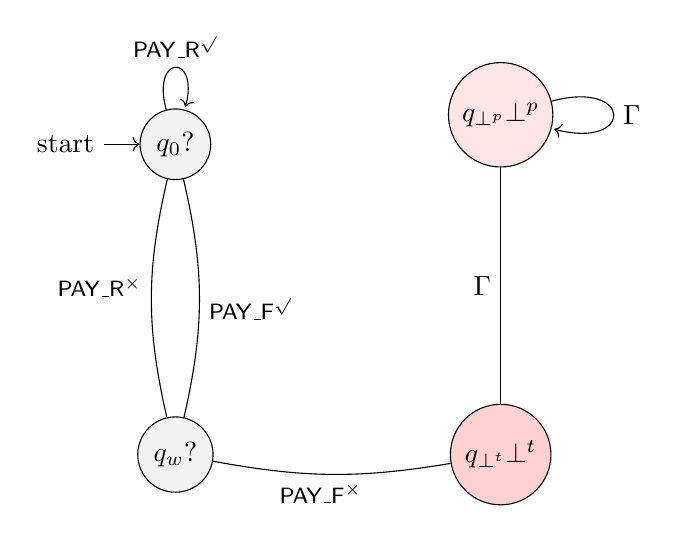
\begin{tikzpicture}
  \node[initial,state,fill=gray!10]          (q0)  {$q_0$\\$\mathsf{?}$};
  \node[state,fill=gray!10,below=3cm of q0]      (qw)  {$q_w$\\$\mathsf{?}$};
  \node[state,fill=red!18,right=3cm of qw]       (qv)  {$q_{\bott}$\\$\bott$};
  \node[state,fill=red!10,above= 3cm of qv]       (qpv) {$q_{\botp}$\\$\botp$};

  \path
    % In-cycle behavior:
    (q0) edge[loop above] node[above,pos=0.5] {\footnotesize $\PAY^\surd$} ()
    (q0) edge[bend right=13] node[left,pos=0.45] {\footnotesize $\PAY^\times$} (qw)
    (qw)  edge[bend right=13] node[right,pos=0.45] {\footnotesize $\PAYF^\surd$} (q0) % restart on tight success
    (qw)  edge[bend right=10] node[below,pos=0.45] {\footnotesize $\PAYF^\times$} (qv)
    % Failure sink:
    (qv)  edge node[left] {$\Gamma$} (qpv)
    (qpv) edge[loop right] node {$\Gamma$} ();
\end{tikzpicture}
\caption{Monitor for $\repit{C_3}$.}
\label{fig:rep-c3_vertical}
\end{subfigure}



\vspace{3mm}
\begin{subfigure}[t]{0.94\textwidth}
\centering
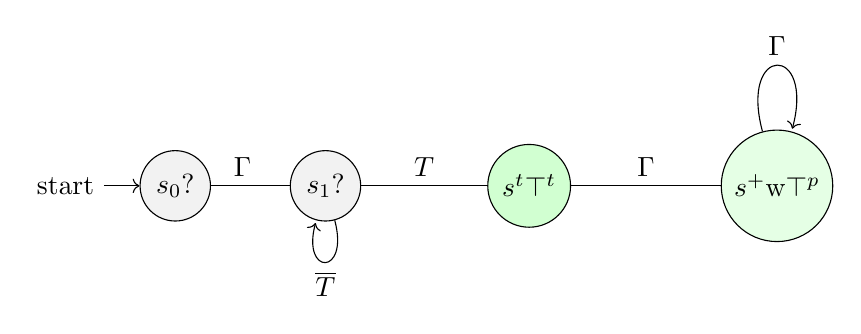
\begin{tikzpicture}
\node[initial,state,fill=gray!10]  (s0)  {$s_0$\\[0.2pt]$\mathsf{?}$};
\node[state,fill=gray!10,right=of s0]  (g)   {$s_1$\\[0.2pt]$\mathsf{?}$};
\node[state,fill=green!18,right=16mm of g] (acc) {$s^t$\\[0.2pt]$\topt$};
\node[state,fill=green!10,right=19mm of acc] (ap) {$s^{+}$\\[0.2pt]w$\topp$};

% --- Transitions ---
\path
  (s0) edge node[above,pos=0.4] {$\Gamma$} (g)
  (g) edge[loop below] node[below] {$\overline{T}$} ()
  (g) edge node[above] {$T$} (acc)
%   (t2) edge node[left,pos=0.5] {$\Gamma$} (acc)
  (acc) edge node[above] {$\Gamma$} (ap)
  (ap) edge[loop above] node {$\Gamma$} ();

\end{tikzpicture}
\caption{Monitor for the regular expression  $\Gamma^+ \cdot  \ \{terminate^{(1)}\}$.}
\label{fig:guard-}
\end{subfigure}
\vspace{3mm}

% -----------------------------------------
% (b) Guarded: guard[re_C5]{rep(C3)} — full width
% -----------------------------------------


\begin{subfigure}[t]{0.94\textwidth}
\centering
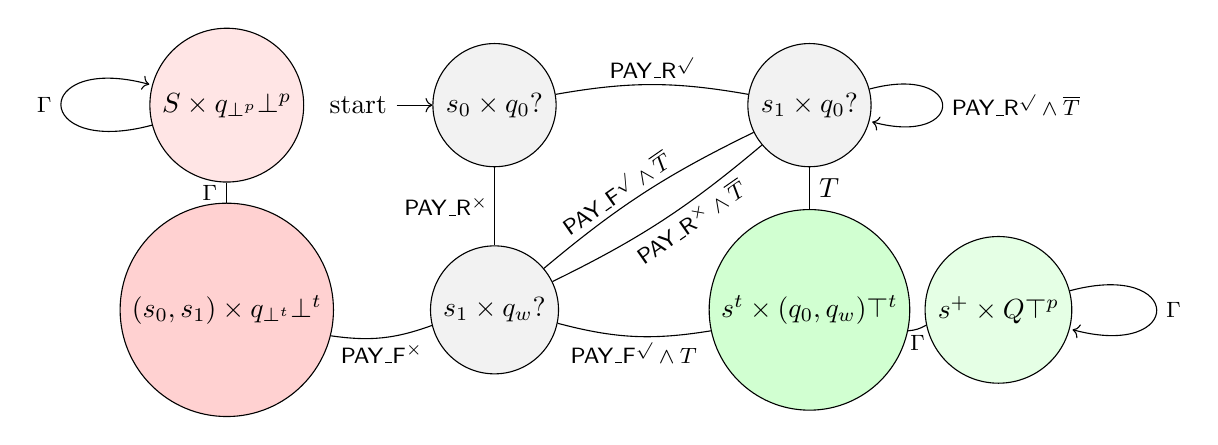
\begin{tikzpicture}

% --- Columns: Bad (x=-3) | ? (x=0) | Accept (x=+3) ---

% ? column (Open, undecided)
\node[initial,state,fill=gray!10]  (Oq0)  at (0, 0) {$s_0\times q_0$\\[0.2pt]$\mathsf{?}$};
\node[state,fill=gray!10]          (Oqw)  at (0,-2.6) {$s_1\times q_w$\\[0.2pt]$\mathsf{?}$};

\node[state,fill=gray!10]  (Oqq00)  at (4, 0) {$s_1\times q_0$\\[0.2pt]$\mathsf{?}$};
%\node[state,fill=gray!10]          (Oqw0)  at (3,-2) {$\text{Open}\times q_w$\\$\mathsf{?}$};

% Bad column (left): tight/post violation sinks
\node[state,fill=red!18]           (Oqv)  at (-3.4,-2.6) {$(s_0,s_1)\times q_{\bott}$\\[0.2pt]$\bott$};
\node[state,fill=red!10]           (Oqpv) at (-3.4, 0) {$S \times q_{\botp}$\\[0.2pt]$\botp$};

% Accept column (right): guard impossible (vacuous accept)
\node[state,fill=green!18]         (Iq0t) at (4, -2.6) {$s^t\times (q_0,q_w)$\\[0.2pt]$\topt$};
\node[state,fill=green!10]         (Iqwt) at (6.4,-2.6) {$s^+\times Q$\\[0.2pt]$\topp$};

% --- Open-region transitions (guard open; C repeats) ---
\path
  %(Oq0) edge[loop above] node {\scriptsize $\overline T$ or $\PAY^\surd$} ()
  (Oq0) edge node[left, inner sep=2pt]{\footnotesize$\PAY^\times$} (Oqw)
  (Oqw) edge[bend left=14] node[below, inner sep=2pt]{\footnotesize $\PAYF^\times$} (Oqv)
 % (Oqw) edge[bend left=12] node[left]{\scriptsize $\PAYF^\surd$} (Oq0)
  (Oqv) edge              node[left] {\footnotesize$\Gamma$} (Oqpv)
  (Oqpv) edge[loop left]  node {\footnotesize$\Gamma$} ();

% --- Mode switches: Open -> Imposs (guard hits bott/botp) ---
\path
  (Oq0) edge[bend left=10]  node[above, inner sep=2pt]{\footnotesize$\PAY^\surd$} (Oqq00)
  (Oqw) edge [bend left=7] node[sloped,above, inner sep=2pt,pos=0.4]{\footnotesize $\PAYF^\surd \wedge \overline{T}$} (Oqq00)
  (Oqq00) edge  [bend left=7] node[sloped,below,inner sep=2pt,pos=0.4] {\footnotesize $\PAY^\times \wedge \overline{T}$} (Oqw)
  
  (Oqq00) edge  node[right] {$T$} (Iq0t)
  (Oqw) edge[bend right=12]  node[below, inner sep=2pt]{\footnotesize $\PAYF^\surd \wedge T$} (Iq0t)
  (Iq0t) edge[bend right=12]  node[below, inner sep=2pt]{\footnotesize $\Gamma$} (Iqwt);
  %(Oq0) edge[bend left=14]  node[below,sloped] {\scriptsize guard $\botp$} (Iqwt)
  %(Oqw) edge[bend left=16]  node[below,sloped] {\scriptsize guard $\botp$} (Iqwt);

% --- Imposs region loops ---
\path
 % (Iq0t) edge[loop right] node {$\Gamma$} ()
  (Iqwt) edge[loop right] node {\footnotesize$\Gamma$} ()
  (Oqq00) edge[loop right] node {\footnotesize$\PAY^\surd \wedge \overline{T}$} ();

\end{tikzpicture}
\caption{Tight satisfaction monitor construction for $\guard[\Gamma^+ \cdot \notifterm^{(1)}]{\repit{C_3}}$.}
\label{fig:guard-repC3}
\end{subfigure}
\caption{%
Progressive construction for $\guard[(\Gamma^+ \cdot \notifterm^{(1)})]{\repit{C_3}}$.
Figure (c) is obtained by applying $\tsmc_\guardd$ to Figures (b) and (a).
Here, roughly speaking, $\PAY^\surd := \{\,A\in\Gamma \mid \{\PAY^{(1)},\PAY^{(2)}\}\subseteq A\,\}$ denotes a joint payment event,$\PAY^\times := \Gamma \setminus \PAY^\surd $ denotes failure of payment.
$T := \{\,A\in\Gamma \mid \notifterm^{(1)}\in A\,\}$ denotes the occurrence of a termination notice by agent~1,
and $\overline{T} := \Gamma\setminus T$ denotes its absence.
}
\label{fig:one-per-line}
\end{figure}



The guarded open-ended contract illustrates how the automaton constructions combine.  
The unbounded repetition of \(C_3\) enforces an indefinite sequence of payments with repair, and the regular expression \(re\) recognizes the first occurrence of a termination notice.  
The guarded product synchronizes both behaviors: while the guard is open, all failures of \(\repit{C_3}\) propagate to the global verdict; once the guard closes, the open-ended obligation is discharged, and the monitor collapses to post acceptance provided that no violation has occurred.  
This example shows that the tight constructions scale to nested patterns of sequencing, repetition, guarding, and reparation while still preserving a direct correspondence with the prefix semantics of \cDL.

\subsection{Forward-Looking Blame Semantics}
The tight semantics of \cDL identify when a contract is satisfied or violated, but do not explain \emph{who} caused a violation.  
To attribute responsibility, we refine the violation verdicts based on which party failed to meet the relevant normative requirement.  
We break down tight and post violations into those caused by agent 1, those caused by agent 2, those caused jointly by both, and those where neither party is responsible (blameless cases).  
Formally, we introduce tight violation verdicts
\[
\bottp{\{1\}},\quad \bottp{\{2\}},\quad \bottp{\{1,2\}},\quad \bottp{\emptyset},
\]
and their post-violation counterparts
\[
\botpp{\{1\}},\quad \botpp{\{2\}},\quad \botpp{\{1,2\}},\quad \botpp{\emptyset}.
\]
By replacing the undifferentiated violation verdicts of the five-valued semantics with these responsibility-aware variants, and keeping the three non-violating verdicts \(\mathsf{?},\topt,\topp\), we obtain the forward-looking blame eleven-valued semantics
\[
  \mathbb{V}_{11} = \{\mathsf{?},\topt,\topp\} \cup \{\bot^{t}_{S},\bot^{p}_{S} \mid S\subseteq \{1,2\}\}.
  \]
This refined judgement structure allows the monitors constructed in the next section to pinpoint the agents responsible for each contractual breach.


\subsubsection*{Blame Rules for Literals}
\begin{definition}[Blame assignment for literals]
Let $p\in\{1,2\}$ be the main subject of the norm and let $\barp$ denote the other party.
Let $\trace{A}$ be a single-step word with $A\in\Gamma$. We write $a^{(i)}\in A$ when party $i$ attempts $a$ in this step.

\paragraph{Obligation \(\obl[p]{a}\).}
Violation occurs if and only if the joint execution does not happen. Blame principle:
if the subject does not attempt, blame the subject; otherwise, blame the other party for not cooperating:
\[
\begin{aligned}
\trace{A}\ \vDash_{\bottp{\{p\}}}\ \obl[p]{a} \;&\mydef\; a^{(p)}\notin A,\\
\trace{A}\ \vDash_{\bottp{\{\barp\}}}\ \obl[p]{a} \;&\mydef\; a^{(p)}\in A\ \land\ a^{(\barp)}\notin A.
\end{aligned}
\]
These two cases partition a tight violation of $\obl[p]{a}$.

\paragraph{Prohibition \(\frb[p]{a}\).}
Violation requires the joint act to occur. Since the subject should refrain, blame the subject:
\[
\trace{A}\ \vDash_{\bottp{\{p\}}}\ \frb[p]{a}\ \;\mydef\;\ \{a^{(1)}, a^{(2)}\}\subseteq A.
\]
If only one agent attempts the action, it does not violate a prohibition, so no other possible blame arises. An agent cannot be blamed for a prohibition that was not assigned to it.

\paragraph{Power \(\perm[p]{a}\).}
Blame occurs only when the subject of the power attempts and the other party withholds cooperation, and the blame goes to the other party:
\[
\trace{A}\ \vDash_{\bottp{\{\barp\}}}\ \perm[p]{a}\ \;\mydef\;\ a^{(p)}\in A\ \land\ a^{(\barp)}\notin A.
\]

\paragraph{Invalid ($\bot$) is blameless.}
\(\lnot(\trace{A}\vDash_{\bottp{S}}\top)\) for all $S$. 
\(\trace{A}\vDash_{\bottp{\emptyset}}\bot\) by convention (unsatisfiable literal with no party subject).

\paragraph{Post violation (prefix closure of blame).}
Tight blame persists to extensions, and post blame is exactly “some earlier tight blame”:
\[
\trace{A}\ \vDash_{\bottp{S}}\ \ell\ \Longrightarrow\ 
\forall\,\pi\ne\emptytrace:\ \trace{A}\concat\pi\ \vDash_{\botpp{S}}\ \ell
\]
\end{definition}

\begin{remark}[No joint blame at the literal level]
    Each literal is decided on a single step, and the only responsibility split is between the subject and the other party:
    either the subject fails to attempt, or the other party fails to cooperate, or no violation occurs. Hence, for literals, the blame set is always a singleton \(S\in\{\{1\},\{2\}\}\) (or empty for \(\bot\)), never \(\{12\}\).
\end{remark}


\begin{example}[Obligation, prohibition, and power blame]
By fixing $p=1$, $\barp=2$. Consider the following letters $A\in\Gamma$:

\smallskip
\noindent\emph{Obligation \(\obl[1]{a}\).}
\[
\begin{array}{lcl}
A=\emptyset: & \trace{A}\ \vDash_{\bottp{\{1\}}}\ \obl[1]{a} & \text{(subject of the obligation did not attempt)}\\
A=\{a^{(2)}\}: & \trace{A}\ \vDash_{\bottp{\{1\}}}\ \obl[1]{a} & \text{(subject did not attempt)}\\
A=\{a^{(1)}\}: & \trace{A}\ \vDash_{\bottp{\{2\}}}\ \obl[1]{a} & \text{(other party did not cooperate)}\\
A=\{a^{(1)},a^{(2)}\}: & \text{no violation} & \text{(joint execution present).}
\end{array}
\]

\noindent\emph{Prohibition \(\frb[1]{a}\).}
\[
\begin{array}{lcl}
A=\{a^{(1)},a^{(2)}\}: & \trace{A}\ \vDash_{\bottp{\{1\}}}\ \frb[1]{a} & \text{(subject should have refrained)}\\
A=\{a^{(1)}\} \quad: & \text{no violation} & \text{The prohibited action was not successful}
\end{array}
\]

\noindent\emph{Power \(\perm[1]{a}\).}
\[
\begin{array}{lcl}
A=\{a^{(1)}\}: & \trace{A}\ \vDash_{\bottp{\{2\}}}\ \perm[1]{a} & \text{(subject asked, other party withheld)}\\
A=\{a^{(1)},a^{(2)}\}: & \text{no violation} & \text{(properly supported)}\\
A=\{a^{(2)}\}: & \text{no violation} & \text{(no unsupported subject attempt).}
\end{array}
\]
\end{example}

\subsubsection*{Blame Propagation in Contracts}
\paragraph{Conjunction.}
For $S \subseteq\{1, 2\}$ of agent(s), and  two contract $C$ and $C'$ from \cDL and a synchronous trace $\pi$, blame is defined for the conjunction $C \wedge C'$ is defined as:
\[
\pi\ \vDash_{\bottp{S}}\ (C\wedge C') \;\iff\;
\begin{cases}
\pi\ \vDash_{\bottp{S}}\ C \ \nd\ \pi \vDash_{\dbot} C',\\[2pt]
\pi\ \vDash_{\bottp{S}}\ C' \ \nd\ \pi \vDash_{\dbot} C,\\[2pt]
\pi\ \vDash_{\bottp{S_1}}\ C\ \nd\ \pi\ \vDash_{\bottp{S_2}}\ C' \text{ with } S=S_1\cup S_2.
\end{cases}
\]
Where $\dbot$ stand for a non violation verdict, i.e, $\dbot \in \{\,?,\ \topp,\ \topt\,\}$\\
\emph{Intuition.}
The three cases summarize the possible outcomes of forward-looking blame.
The blame goes to the agent responsible for the first violation of the contract: so either C or C', but both contracts could be violated at the same time point, in this case, the agent or agents responsible for \emph{both simultaneous} violation get the blame.

For the rest of the operators,  blame  follows a similar definition as the tight violation, with $k \in [0, \size{\pi}]$:

\paragraph{Sequence.}
For \(S\subseteq\{1,2\}\), contracts \(C,C'\) in \cDL, and a synchronous trace \(\pi\):
\[
\pi\ \vDash_{\bottp{S}}\ (C;C') \;\iff\;
\begin{cases}
\pi\ \vDash_{\bottp{S}}\ C,\\[2pt]
\exists \pi_k\ \vDash_{\topt} \ C \ \nd\ \pi^{k}\ \vDash_{\bottp{S}}\ C'.
\end{cases}
\]
\emph{Intuition.} The first decisive failure before \(C\) has tightly succeeded belongs to \(C\), so its blame propagates. Once \(C\) has tightly succeeded (\(\topt\)) or is in post-success (\(\topp\)), only \(C'\) can still fail, so the blame comes from \(C'\). There is no tie, since \(C'\) becomes active only after \(C\) has tightly succeeded.

\paragraph{Reparation.}
For \(S\subseteq\{1,2\}\), the blame for a reparation contract \(C\repair C'\) is defined as:
\[
\pi\ \vDash_{\bottp{S}}\ (C\repair C')
\;\iff\;
\exists\,k\ \text{such that}\ 
\pi_k\ \vDash_{\bott}\ C
\ \nd\
\pi^k\ \vDash_{\bottp{S}}\ C'.
\]
\emph{Intuition.}  A reparation clause becomes active only after a violation of \(C\). The global blame set \(S\), therefore, corresponds to the agents responsible for violating the reparation \(C'\) once it is triggered. The blame for $C$ is not considered, as one cares only for the overall violation of the combined contracts.


\begin{example}[Witness traces for all blame verdicts]
We use $\Sigma_C=\{\PAY,\PAYF,\OCC\}$ and letters $A_t\subseteq\Gamma$ with agent tags $\cdot^{(1)},\cdot^{(2)}$.
Recall
\[
C_2' := \perm[1]{\OCC}\ ;\ \perm[1]{\OCC},\qquad
C_3 := \obl[1]{\PAY}\ \repair\ \obl[1]{\PAYF}.
\]


\medskip
\noindent\textbf{Tight blame for agent 1 }
\[
\pi_1=\langle A_0\rangle,\quad A_0=\{\OCC^{(1)}\}
\]
Here, $\perm[1]{\OCC}$ and $ \obl[1]{\PAY}$ are violated, the blame verdicts are:
\begin{itemize}
\item The tenant (1) gets blamed for violating the obligation to pay rent:\\ $\pi_1 \vDash_{\bottp{\{1\}}} \obl[1]{\PAY}$. 
\item The landlord (2) gets blamed for violating the power of the tenant to occupy the flat:\\
$\pi_1 \vDash_{\bottp{\{2\}}} \perm[1]{\OCC}$.
\end{itemize}
But the specification allows for the reparation $\obl[1]{\PAY}\ \repair\ \obl[1]{\PAYF}$. So consequently, no tight violation can be diagnosed at $T=1$:\\
$\pi_1 \presat \obl[1]{\PAY}\ \repair\ \obl[1]{\PAYF}.$
Consequently, only the landlord gets the blame for the overall specification:
\[\pi_1 \vDash_{\bottp{\{2\}}} C_2' \wedge C_3.\]

Moreover, consider the trace of  $\pi_2:= \trace{\{\OCC^{(1)}\}, \{\OCC^{(1)}\}}$, the extension of $\pi_1$ with the same event, as the blame is forward and tight looking, the blame is still assigned only to agent $2$ (landlord) as they is responsible for the first violation.

Let us consider instead the following trace $\pi_3:=\trace{A_0',A_1}$ with $A_0':= \{\OCC^{(1)}, \OCC^{(2)}\}$ and $A_1:= \{\OCC^{(1)}\}$.

Here:
\begin{itemize}
\item The landlord gets the blame at $T=2$ for violating the power of the tenant to occupy the flat in the second month:\\
$\pi_3 \vDash_{\bottp{\{2\}}} \perm[1]{\OCC}\ ;\ \perm[1]{\OCC} $.
\item For the reparation clause $\obl[1]{\PAY}\ \repair\ \obl[1]{\PAYF}$ we must distinguish two different situations in which the fine is not honored:
  \begin{itemize}
    \item if the tenant never attempts to pay the fine, that is, no letter of the trace contains $\PAYF^{(1)}$, then the blame goes to agent 1:\\
    $\pi \vDash_{\bottp{\{1\}}} \obl[1]{\PAY}\ \repair\ \obl[1]{\PAYF}$,
    \item if instead the tenant attempts to pay the fine and the landlord does not cooperate, for example, in a letter $A$ with $\PAYF^{(1)}\in A$ and $\PAYF^{(2)}\notin A$, then the fine obligation is violated, and the blame goes to agent 2:\\
    $\pi \vDash_{\bottp{\{2\}}} \obl[1]{\PAY}\ \repair\ \obl[1]{\PAYF}$.
  \end{itemize}
\end{itemize}
\end{example}

\begin{lemma}[Tight forward blame is deterministic]
\label{lem:blame-deterministic}
For every trace $\pi\in\Gamma^*$ and every contract $C$ in \cDL, there exists a unique verdict
$v\in\mathbb{V}_{11}$ such that $\pi\ \vDash_{v}\ C$.
Equivalently, for all $v,v'\in\mathbb{V}_{11}$,
\[
\pi\ \vDash_{v}\ C\ \land\ \pi\ \vDash_{v'}\ C\ \Longrightarrow\ v=v'.
\]
\end{lemma}

\begin{proof}
By structural induction on $C$.

\paragraph{Literals.}
For $C=\ell$, the blame rules in Definition~\ref{def:lockstep-hs} distinguish violations by a finite case split on the current letter $A\in\Gamma$.
In each case, at most one blame set is applicable.
For instance, for $\obl[p]{a}$, either $a^{(p)}\notin A$ (yielding $\bottp{\{p\}}$), or $a^{(p)}\in A\land a^{(\bar p)}\notin A$ (yielding $\bottp{\{\bar p\}}$), or the joint act occurs (no violation).
The clauses for $\frb[p]{a}$ and $\perm[p]{a}$ are analogous.
Post blame is uniquely determined because $\botpp{S}$ holds exactly when some earlier prefix had the corresponding tight blame $\bottp{S}$.

\paragraph{Boolean and temporal constructors.}
Assume determinism holds for strict subcontracts.
For conjunction $C_1\wedge C_2$, the inductive hypothesis yields unique verdicts $v_1$ and $v_2$ for $C_1$ and $C_2$ on $\pi$.
The conjunction clause then produces a unique combined verdict: if exactly one side is a tight (or post) blame verdict, it is selected; if both are blame verdicts, the blame set is uniquely $S_1\cup S_2$; otherwise the result is the unique non-violating combination.

For sequence $C_1;C_2$, the semantics activates $C_2$ only after $C_1$ reaches tight success ($\topt$) and otherwise propagates the unique verdict of $C_1$.
Thus there is no ambiguity between blaming $C_1$ and blaming $C_2$.

For reparation $C_1\repair C_2$, the repair is triggered by the first decisive violation of $C_1$.
The triggering point is unique because the underlying tight regions are prefix-monotone, and the inductive hypothesis yields a unique verdict for the suffix evaluated against $C_2$.
Hence the overall blame verdict is unique.

All remaining constructors follow the same pattern: control flow is determined by the underlying tight verdicts, and blame information is carried along deterministically by the inductive hypothesis.
Therefore, for every $\pi$ and $C$, exactly one verdict in $\mathbb{V}_{11}$ applies.
\end{proof}

\begin{theorem}[Tight Forward Blame semantics is a refinement of tight forward satisfaction]
The tight forward semantics is a refinement of forward tight semantics, that is for any contract $C$ from \cDL and $\pi$ over $\Gamma^*$, we have:
\[
\semfive{\pi,C}=
\begin{cases}
? & \text{ iff } \semelf{\pi,C}=?,\\
\topt & \text{ iff }   \semelf{\pi,C}=\topt,\\
\topp & \text{ iff }  \semelf{\pi,C}=\topp,\\
\bott & \text{ iff }  \exists!\,S\subseteq \{1,2\}:\ \semelf{\pi,C}= \bottp{S},\\
\botp & \text{ iff }  \exists!\,S\subseteq \{1,2\}:\ \semelf{\pi,C}= \botpp{S}.\\
\end{cases}
\]
\end{theorem}

\begin{proof}
    We prove the statement by structural induction on the contract $C$.
    
    \paragraph{Base case: literals.}
    Let $C=\ell$ be a literal, and let $\pi\in\Gamma^*$ be a finite trace.
    
    \smallskip
    \noindent\emph{Case $|\pi|=0$.}
    By Definition~\ref{def:lattsat}, we have $\emptytrace\ \presat\ \ell$ for every literal $\ell$.
    Hence the corresponding five-valued verdict is the undecided one, namely $\semfive{\emptytrace,\ell}=?$.
    On the blame side, there is no letter to trigger any tight blame clause, and post blame is defined only from an earlier tight blame.
    Therefore $\semelf{\emptytrace,\ell}=?$.
    This establishes the three non-violating cases in the displayed refinement table for $\pi=\emptytrace$.
    
    \smallskip
    \noindent\emph{Case $|\pi|\ge 1$.}
    Write $\pi=\trace{A}\concat \pi'$ with $A\in\Gamma$.
    
    First, consider the five-valued semantics. By Definition~\ref{def:lattsat}, literals are decided on the first letter:
    exactly one of $\trace{A}\ \satt\ \ell$ or $\trace{A}\ \violt\ \ell$ holds.
    
    Now consider the blame semantics for literals (your Definition “Blame assignment for literals”).
    If $\trace{A}\ \satt\ \ell$, then no blame violation verdict applies at the first step, so $\semelf{\pi,\ell}\in\{?,\topt,\topp\}$ and the collapse leaves it unchanged. Hence $\semfive{\pi,\ell}\in\{?,\topt,\topp\}$ matches the same non-violating region.
    
    If instead $\trace{A}\ \violt\ \ell$, then by your literal blame rules the violation is refined into a (unique) blame set $S\subseteq\{1,2\}$:
    for $\obl[p]{a}$ there are exactly the two exclusive cases
    $a^{(p)}\notin A$ and $a^{(p)}\in A\land a^{(\bar p)}\notin A$,
    for $\frb[p]{a}$ there is the single case $\{a^{(1)},a^{(2)}\}\subseteq A$,
    and for $\perm[p]{a}$ there is the single case $a^{(p)}\in A\land a^{(\bar p)}\notin A$.
    Thus $\semelf{\pi,\ell}=\bottp{S}$ at the decisive step and, by the post clause, $\semelf{\trace{A}\concat\pi',\ell}=\botpp{S}$ for every non-empty suffix $\pi'$.
    Collapsing erases $S$, yielding $\bott$ at the tight step and $\botp$ afterwards, which is exactly the five-valued classification of a literal (tight violation at the first letter, then post violation).
    Hence the refinement statement holds for literals.
    
    \paragraph{Inductive step.}
    Assume the statement holds for all strict subcontracts of $C$ (and for the required suffix evaluations in the operators that split the trace).
    We show it holds for $C$ by considering the outermost constructor.
    
    \paragraph{Conjunction $C=C_1\wedge C_2$.}
    By the inductive hypothesis, for each $i\in\{1,2\}$ the blame verdict on $C_i$ collapses to the five-valued verdict on $C_i$.
    In the blame semantics, the only difference from the five-valued semantics is that whenever a violation occurs, it carries a blame set, and when both sides violate at the same decisive point, the blame sets are unioned.
    Erasing the blame set therefore yields exactly the same coarse outcome as in the five-valued semantics:
    non-violating combinations stay in $\{?,\topt,\topp\}$, tight blame collapses to $\bott$, and post blame collapses to $\botp$.
    Hence the equivalence holds for $C_1\wedge C_2$.
    
    \paragraph{Sequence $C=C_1;C_2$.}
    Both semantics use the same control flow: $C_2$ is evaluated only after the unique split point where $C_1$ reaches tight success, and otherwise the verdict is inherited from $C_1$.
    The blame semantics again only refines violations by attaching a blame set.
    By the inductive hypothesis on $C_1$ and on $C_2$ evaluated on the suffix beyond the split, collapsing the blame verdict yields exactly the five-valued verdict for $C_1;C_2$.
    
    \paragraph{Reparation $C=C_1\repair C_2$.}
    Both semantics activate $C_2$ precisely at the first tight violation of $C_1$.
    The five-valued semantics records only whether the composite ends in $\bott$ or $\botp$ (or remains non-violating), while the blame semantics records the same region but decorates violation with a blame set.
    By the inductive hypothesis for $C_1$ and for $C_2$ on the triggered suffix, erasing the blame set yields the same coarse verdict as in the five-valued semantics.
    Hence the equivalence holds for $C_1\repair C_2$.
    
    \paragraph{Repetition and regex constructors.}
    For $C^n$, $\repit{C}$, $\trig[re]{C}$, and $\guard[re]{C}$, the blame clauses mirror the five-valued clauses and differ only by refining violation outcomes with blame sets (and propagating them to the post region).
    Applying the inductive hypothesis to the involved subcontracts (and to the required suffixes) and then erasing the blame sets yields the corresponding five-valued verdict in each case.
    
    Thus all constructors preserve the refinement property. Therefore the statement holds for all contracts $C$.
    \end{proof}

\subsection{From Tight Contract Satisfaction Monitor to Tight Blame Monitor}

In the previous subsection, we defined a denotational blame semantics that refines tight and post violations by assigning responsibility to one or both agents. We now show that this refinement can be realized operationally.
Unlike the tight satisfaction monitor, which groups all violations into a single generic $\bott$ verdict, the blame monitor must distinguish between different causes of violation.
Therefore, we cannot simply relabel the outputs of the existing monitor; we must construct a new monitor whose state space explicitly encodes these distinctions.

\begin{definition}[Blame monitor]
\label{def:blamemonitor}
The \emph{blame monitor}, written $\mathcal{M}_{11}$, is a Moore machine whose output alphabet is the eleven-valued blame verdict set $\mathbb{V}_{11}$. Formally,
\[
\mathcal{M}_{11} = (Q,q_0,\Gamma,\mathbb{V}_{11},\delta,\lambda_{11}),
\]
where:
\begin{enumerate}
  \item The output alphabet is
  \[
    \mathbb{V}_{11} = \{\mathsf{?},\topt,\topp\} \cup \{\bot^{t}_{S},\bot^{p}_{S} \mid S\subseteq \{1,2\}\}.
  \]
  \item $Q$ is the set of states and $q_0\in Q$ is the initial state,
  \item $\Gamma = 2^\Sigma$ is the input event alphabet,
  \item $\delta: Q \times \Gamma \to Q$ is the transition function,
  \item $\lambda_{11}: Q \to \mathbb{V}_{11}$ is the state output function.
\end{enumerate}
\end{definition}

We now define the construction function $\bmc(C)$ inductively. This follows the same structural approach as the tight satisfaction monitor construction $\tsmc(C)$ (Definition~\ref{def:tsmc}), but creates distinct states for distinct blame assignments.

\begin{definition}[Blame Monitor Construction]
\label{def:bmc}
The \emph{blame monitor construction} is a function $\bmc(C)$ defined inductively on the structure of the contract $C$.

\paragraph{Base Case: Literals ($\ell$).}
For any literal $\ell$ (including obligations, permissions, and constants $\top, \bot$), the monitor is defined as:
\[
\bmc_{\mathit{lit}}(\ell) = (Q_{\ell}, q_0, \Gamma, \mathbb{V}_{11}, \delta_{\ell}, \lambda_{11}).
\]
\begin{itemize}
    \item \textbf{State Space:} The set $Q_{\ell}$ contains a start state, success states, and specific blame states for any valid blame set $S$ associated with $\ell$ (where $S=\emptyset$ for $\bot$):
    \[
    Q_{\ell} = \{q_0, q_s, q_{ps}\} \cup \bigcup_{S} \{q_{\bott}^S, q_{\botp}^S\}.
    \]
    \item \textbf{Transitions:} The initial transition is determined directly by the denotational blame rules on the input letter $A$:
    \[
    \delta_{\ell}(q_0, A) = 
    \begin{cases}
        q_s & \text{if } \trace{A} \satt \ell \quad (\text{always true for } \top), \\
        q_{\bott}^S & \text{if } \trace{A} \vDash_{\bottp{S}} \ell.
    \end{cases}
    \]
    Subsequent transitions capture the irrevocability of the verdicts:
    \[
    \delta_{\ell}(q_s, \Gamma) = q_{ps}, \quad \delta_{\ell}(q_{ps}, \Gamma) = q_{ps}, \quad \text{and} \quad
    \delta_{\ell}(q_{\bott}^S, \Gamma) = q_{\botp}^S, \quad \delta_{\ell}(q_{\botp}^S, \Gamma) = q_{\botp}^S.
    \]
    \item \textbf{Outputs:} $\lambda_{11}$ maps states to their corresponding verdicts:\\
    $q_0 \mapsto \mathsf{?}$, ~~
    $q_s \mapsto \topt$, ~~
    $q_{ps} \mapsto \topp$, ~~
    $q_{\bott}^S \mapsto \bottp{S}$, and ~~
    $q_{\botp}^S \mapsto \botpp{S}$.
\end{itemize}

\paragraph{Inductive Step: Other Operators.}
For Sequence ($C_1 ; C_2$), Reparation ($C_1 \repair C_2$), Repetition ($\nrep(n,C), \repit{C}$), and Guarded contracts, the construction follows the exact same topological logic as the Tight Satisfaction Monitor constructions (Definitions \ref{def:moore-seq} to \ref{def:moore-repeat-unbounded}), with one key adaptation:
\begin{itemize}
    \item \textbf{Matching Blame States:} Wherever the tight monitor construction redirects a generic violation state (outputting $\bott$), the blame monitor construction redirects \emph{all} corresponding specific blame states (outputting $\bottp{S}$ for any $S$).
    \item \textbf{Example (Reparation):} In $\tsmc_{\repair}$, transitions to any state $q$ where $\lambda_5(q)=\bott$ are redirected to the initial state of $C_2$. In $\bmc_{\repair}$, transitions to \emph{any} state $q$ where $\lambda_{11}(q)=\bottp{S}$ (regardless of $S$) are redirected to the initial state of $C_2$.
\end{itemize}
This preserves the control-flow semantics of the operators: for example, in reparation, \emph{any} fault by \emph{any} party in the primary contract triggers the secondary contract, effectively masking the initial blame in favor of the reparation's outcome.
\end{definition}

\begin{theorem}[Correctness of the Blame Monitor]
\label{thm:bm-correct}
Let $C$ be a contract in \cDL. For every finite trace $\pi$, the output of the blame monitor $\bmc(C)$ equals the denotational blame verdict:
\[
\lambda_{11}\bigl(\delta(q_0,\pi)\bigr) = \mathsf{Blame}(C,\pi).
\]
\end{theorem}

\begin{proof}
The proof proceeds by structural induction on $C$.
\begin{itemize}
    \item \textbf{Literals:} The state splitting in $\bmc_{\mathit{lit}}$ explicitly encodes the blame partition rules. For $\obl[p]{a}$, the transition $\delta_{\ell}$ ensures that a trace with $a^{(p)} \notin A$ reaches $q_{\bott}^p$, while a trace with blocked cooperation reaches $q_{\bott}^{\bar{p}}$. This matches the semantic definition.
    \item \textbf{Conjunction:} The product construction explores all pairs of states. The definition of $\lambda_{11}^{\wedge}$ explicitly calculates $S_1 \cup S_2$ when both components are in violation states, and selects the single responsible party when only one violates. This matches the semantic clause $\pi \vDash_{\bottp{S_1 \cup S_2}} C_1 \wedge C_2$.
    \item \textbf{Other Operators:} The correctness relies on the fact that operators like Sequence and Reparation are defined by switching control based on the \emph{presence} of a violation (or success), not the \emph{content} of the blame.
    For instance, in $C_1 \repair C_2$, the semantics state that if $C_1$ fails (regardless of $S$), we evaluate $C_2$. The monitor construction realizes this by redirecting all transitions targeting any $\bottp{S}$-labeled state of $C_1$ to the start of $C_2$. Thus, the initial blame $S$ is discarded (masked) exactly as prescribed by the semantics, and the final verdict is determined by $C_2$.
\end{itemize}
\end{proof}

% \begin{definition}[Blame monitor]
% \label{def:blamemonitor}
% The \emph{blame monitor}, written $\mathcal{M}_{11}$, is a Moore machine whose output alphabet is the eleven-valued blame verdict set $\mathbb{V}_{11}$. Formally,
% \[
% \mathcal{M}_{11} = (Q',q_0,\Gamma,\mathbb{V}_{11},\delta',\lambda_{11}),
% \]
% where:
% \begin{enumerate}
%   \item $\mathbb{V}_{11} = \{\mathsf{?},\topt,\topp\} \cup \{\bot^{t}_{S},\bot^{p}_{S} \mid S\in\{\{0\},\{1\},\{2\},\{12\}\}\}$,
%   \item $Q'$ is the refined set of states,
%   \item $\delta': Q' \times \Gamma \to Q'$ is the refined transition function,
%   \item $\lambda_{11}: Q' \to \mathbb{V}_{11}$ is the state output function.
% \end{enumerate}
% \end{definition}

% \begin{definition}[Blame monitor construction]
%     \label{def:bmc}
%     Let $C$ be a contract in \cDL. The \emph{blame monitor construction}, denoted $\bmc(C)$, refines the tight satisfaction monitor
%     \[\tsmc(C) = (Q,q_0,\Gamma,\tightverdicts,\delta,\lambda_5)\]
%    into the blame monitor defined as:
%    \[
%    \bmc(C) := (Q',q_0,\Gamma,\mathbb{V}_{11},\delta',\lambda_{11}).
%    \]
%    The state space $Q$ is partitioned into $Q'$ via a refinement map $\mathcal{R}: Q \to \mathcal{P}(Q')$ such that generic violation states in $Q$ are split into distinct blame states in $Q'$.
%    The transition function $\delta'$ and output function $\lambda_{11}$ are defined inductively on the structure of $C$
%     \end{definition}
    
%     \begin{theorem}[Correctness and Consistency of the Blame Monitor]
%     \label{thm:bm-correct}
%     Let $C$ be a contract in \cDL. Let $\tmon(C)$ be its tight satisfaction monitor and $\mathcal{BM}(C)$ be its blame monitor constructed as per Definition~\ref{def:bmc}.
%     For every finite trace $\pi$:
%     \[
%     \lambda^{\mathcal{BM}}\bigl(\delta^{\mathcal{BM}}(q_0,\pi)\bigr) 
%       \;=\; 
%     \mathsf{Blame}(C,\pi).
%     \]
%     \end{theorem}
        
%     \begin{proof}
%     The proof follows directly from the inductive construction in Definition~\ref{def:bmc}.
%     \begin{itemize}
%         \item \textbf{Literals:} The splitting of the transition function $\delta'$ ensures that traces where the subject is passive lead to $q_p$ (output $\bottp{\{p\}}$), and traces where the counterparty blocks lead to $q_{\bar{p}}$ (output $\bottp{\bar{p}}$). This matches the denotational rule for literals.
%         \item \textbf{Conjunction:} The definition of $\lambda_{11}^{\wedge}$ explicitly implements the union of blame sets ($S_1 \cup S_2$) required by the denotational semantics when multiple violations occur.
%         \item \textbf{Sequence/Reparation:} Since these operators partition the trace into independent segments, the correctness of the sub-monitors (Inductive Hypothesis) guarantees the correctness of the composite monitor.
%     \end{itemize}
%     Thus, $\mathcal{BM}(C)$ correctly implements $\mathsf{Blame}(C, \pi)$ for all $\pi$.
%     \end{proof}

% In all cases, $\lambda_{11}$ correctly maps the state to the specific blame verdict defined by the forward-looking semantics. We now move to illustrate this refinement with two interesting examples.

\begin{example}[Blame Monitor for $C_2 \wedge C_3$]
  Let us recall that $C_2 = \perm[1]{\OCC}$ represents the tenant's power to occupy the property, and $C_3 = \obl[1]{\PAY} \repair \obl[1]{\PAYF}$ represents the obligation to pay rent, repaired by paying a fine.
  The following figure shows the blame refinement of the monitor in Figure~\ref{fig:c2andc3}. The generic violation state is partitioned into specific blame verdicts based on the cause of the failure.
  
  \begin{figure}[h!]
  \centering
  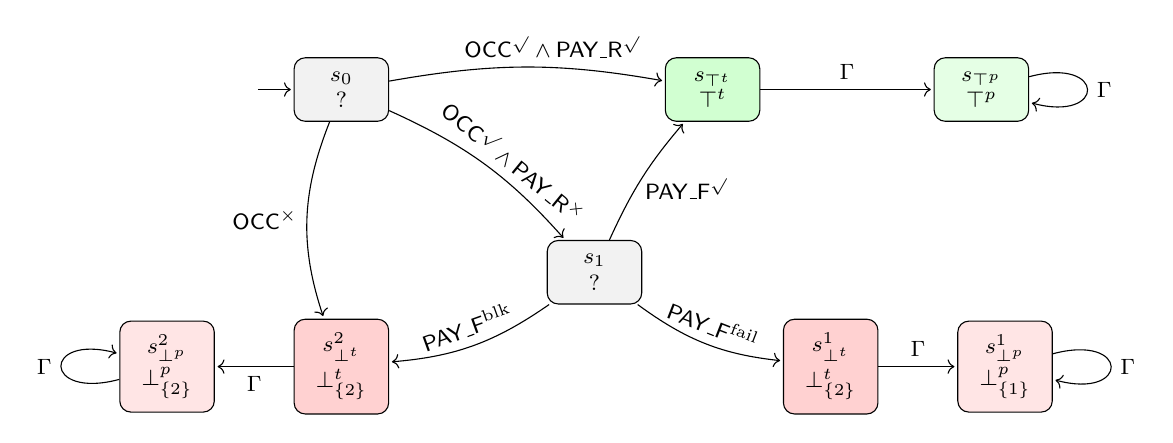
\begin{tikzpicture}[
    ->,shorten >=1pt, node distance=20mm and 18mm,
    every state/.style={
      rectangle,rounded corners,draw,
      minimum width=12mm,minimum height=7mm,
      inner sep=5pt,font=\footnotesize,align=center
    },
    initial text={}
  ]
  
  % --- Non-Violating States (Preserved) ---
  \node[initial,state,fill=gray!10] (q0) {$s_0$\\$\mathsf{?}$};
  \node[state, fill=gray!10, below right=15mm and 20mm of q0] (q1) {$s_1$\\$\mathsf{?}$};
  \node[state,fill=green!18,right=35mm of q0] (qs) {$s_{\topt}$\\$\topt$};
  \node[state,fill=green!10,right=22mm of qs] (qps) {$s_{\topp}$\\$\topp$};
  
  % --- Blame States (Split) ---
  % Blame 2 (Landlord) - e.g., blocking permission or fine
  \node[state,fill=red!18,below=25mm of q0] (qv2) {$s_{\bott}^2$\\[2pt]$\bottp{\{2\}}$};
  \node[state,fill=red!10,left=10mm of qv2] (qpv2) {$s_{\botp}^2$\\ [2pt]$\botpp{\{2\}}$};
  
  % Blame 1 (Tenant) - e.g., failing to pay fine
  \node[state,fill=red!18,right=50mm of qv2] (qv1) {$s_{\bott}^1$\\[2pt]$\bottp{\{2\}}$};
  \node[state,fill=red!10,right=10mm of qv1] (qpv1) {$s_{\botp}^1$\\[2pt]$\botpp{\{1\}}$};
  
  % --- Transitions ---
  
  % 1. Success paths (Unchanged)
  \path
    (q0) edge[bend left=10] node[above,pos=0.6] {\footnotesize$\OCC^\surd \land \PAY^{\surd}$} (qs)
    (q0) edge[bend left=12] node[pos=0.6,sloped,above] {\footnotesize$\OCC^\surd \land \PAY^{\times}$} (q1)
    (q1) edge[bend left=8] node[right,pos=0.4] {\footnotesize$\PAYF^\surd$} (qs)
    (qs) edge node[above] {\footnotesize$\Gamma$} (qps)
    (qps) edge[loop right] node {\footnotesize$\Gamma$} ();
  
  % 2. Violation: Landlord Fault (Blame 2)
  % From s0: Landlord blocks occupation (Violation of P_1(OCC))
  \path
    (q0) edge[bend right=20] node[left,pos=0.5] {\footnotesize$\OCC^{\times}$} (qv2);
  
  % From s1: Landlord blocks fine payment (Violation of O_1(PAY_F))
  % Define specific label for blocked fine: Tenant tries, Landlord blocks
  \path
    (q1) edge[bend left=15] node[above,sloped] {\footnotesize$\PAYF^{\text{blk}}$} (qv2);
  
  % 3. Violation: Tenant Fault (Blame 1)
  % From s1: Tenant fails to pay fine (Violation of O_1(PAY_F))
  % Define specific label for passive failure: Tenant doesn't try
  \path
    (q1) edge[bend right=15] node[above,sloped] {\footnotesize$\PAYF^{\text{fail}}$} (qv1);
  
  % 4. Post-Violation Loops
  \path
    (qv2) edge node[auto] {\footnotesize$\Gamma$} (qpv2)
    (qv1) edge node[auto] {\footnotesize$\Gamma$} (qpv1)
    (qpv2) edge[loop left] node {\footnotesize$\Gamma$} ()
    (qpv1) edge[loop right] node {\footnotesize$\Gamma$} ();
  
  \end{tikzpicture}
  \caption{Blame Monitor $\mathcal{BM}(C_2 \wedge C_3)$.
  \textbf{Changes from Tight Monitor:}
  The state $s_{\bott}$ is split into $s_{\bott}^2$ (Landlord blame) and $s_{\bott}^1$ (Tenant blame).
  \textbf{Edge Definitions:}
  $\OCC^\times$: Tenant attempts $\OCC$, Landlord blocks.
 $\PAYF^{\text{fail}}$: Tenant does not attempt $\PAYF$ ($\PAYF^{(1)} \notin A$).
  $\PAYF^{\text{blk}}$: Tenant attempts $\PAYF$, Landlord blocks.
  }
  \label{fig:blame-monitor}
  \end{figure}
  \end{example}

  Although the previous example is constructed using a conjunction, the reparation operator within $C_3$ delays the assignment of blame for the payment obligation.
Specifically, if the tenant fails to pay rent, the monitor transitions to a waiting state for the repair (outputting $\mathsf{?}$) rather than immediately emitting a violation verdict.
Consequently, it is impossible for both conjuncts to return a tight violation $\bott$ at the same initial step.
To illustrate a scenario where the monitor can output the joint blame verdict $\bottp{12}$, we consider the reparation-free reduction of the specification: $\perm[1]{\OCC} \wedge \obl[1]{\PAY}$.

  \begin{example}[Blame Monitor with double blame]\label{example:joint-blame}
    The following monitor in \ref{fig:joint-blame} shows the emergence of joint blame. From the initial state $s_0$, three distinct violation paths are possible depending on who fails. The path to $s_{\bott}^{12}$ represents the simultaneous failure of both parties.
    
    \begin{figure}[h!]
    \centering
    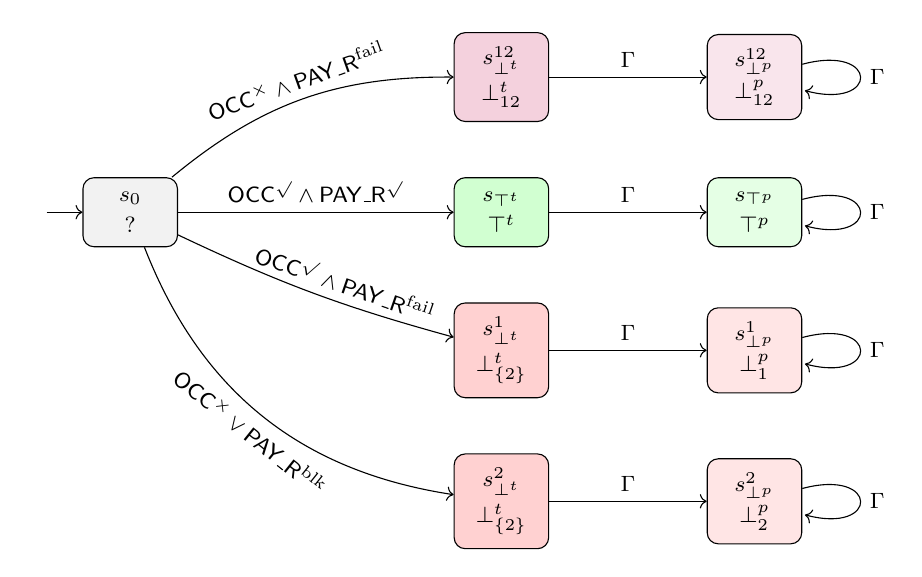
\begin{tikzpicture}[
      ->, node distance=20mm and 25mm,
      every state/.style={
        rectangle,rounded corners,draw,
        minimum width=12mm,minimum height=7mm,
        inner sep=5pt,font=\footnotesize,align=center
      },
      initial text={}
    ]
    
    % --- Initial State ---
    \node[initial,state,fill=gray!10] (q0) {$s_0$\\[2pt]$\mathsf{?}$};
    
    % --- Success State ---
    \node[state,fill=green!18,right=35mm of q0] (qs) {$s_{\topt}$\\[2pt]$\topt$};
    \node[state,fill=green!10,right=20mm of qs] (qps) {$s_{\topp}$\\[2pt]$\topp$};
    
    % --- Violation States ---
    
    % 1. Joint Blame (Top Path)
    \node[state,fill=purple!18,above right=7mm and 35mm of q0] (q12) {$s_{\bott}^{12}$\\[2pt]$\bottp{12}$};
    \node[state,fill=purple!10,right=20mm of q12] (qp12) {$s_{\botp}^{12}$\\[2pt]$\botpp{12}$};
    
    % 2. Tenant Blame (Middle/Right Path)
    \node[state,fill=red!18,below=7mm of qs] (q1) {$s_{\bott}^{1}$\\[2pt]$\bottp{\{2\}}$};
    \node[state,fill=red!10,right=20mm of q1] (qp1) {$s_{\botp}^{1}$\\[2pt]$\botpp{1}$};
    
    % 3. Landlord Blame (Bottom Path)
    \node[state,fill=red!18,below=7mm of q1] (q2) {$s_{\bott}^{2}$\\[2pt]$\bottp{\{2\}}$};
    \node[state,fill=red!10,right=20mm of q2] (qp2) {$s_{\botp}^{2}$\\[2pt]$\botpp{2}$};
    
    % --- Transitions ---
    
    % Success: Tenant pays AND Landlord allows occupation
    \path
      (q0) edge node[above] {\footnotesize$\OCC^\surd \land \PAY^\surd$} (qs)
      (qs) edge node[above] {\footnotesize$\Gamma$} (qps)
      (qps) edge[loop right] node {\footnotesize$\Gamma$} ();
    
    % Joint Violation: Tenant doesn't pay AND Landlord blocks occupation
    \path
      (q0) edge[bend left=20] node[sloped,above] {\footnotesize$\OCC^\times \land \PAY^{\text{fail}}$} (q12)
      (q12) edge node[above] {\footnotesize$\Gamma$} (qp12)
      (qp12) edge[loop right] node {\footnotesize$\Gamma$} ();
    
    % Tenant Violation: Landlord allows occupation, BUT Tenant doesn't pay
    \path
      (q0) edge[bend right=5] node[sloped,above,pos=0.6] {\footnotesize$\OCC^\surd \land \PAY^{\text{fail}}$} (q1)
      (q1) edge node[above] {\footnotesize$\Gamma$} (qp1)
      (qp1) edge[loop right] node {\footnotesize$\Gamma$} ();
    
    % Landlord Violation: Tenant pays, BUT Landlord blocks occupation
    \path
      (q0) edge[bend right=30] node[sloped,below] {\footnotesize$\OCC^\times \vee \PAY^{\text{blk}}$} (q2)
      (q2) edge node[above] {\footnotesize$\Gamma$} (qp2)
      (qp2) edge[loop right] node {\footnotesize$\Gamma$} ();
    
    \end{tikzpicture}
    \caption{Blame Monitor for $\perm[1]{\OCC} \wedge \obl[1]{\PAY}$.\\
    \textbf{Edge Definitions:}\\
    $\PAY^{\text{fail}}$: Tenant does not attempt payment ($\PAY^{(1)} \notin A$).\\
    $\OCC^\times$: Tenant attempts occupation, Landlord blocks.\\ $\PAY^{\text{blk}}$: Tenant attempts to pay and Landlord blocks.\\
    The state $s_{\bott}^{12}$ is reached only when both violations occur in the same step.}
    \label{fig:joint-blame}
    \end{figure}
    \end{example}


    \begin{example}[Blame Monitor for $\repit{C_3}$]
      The figure below shows the blame monitor for the unbounded repetition of the rent-and-reparation contract. The generic violation state $q_{\bott}$ from the standard monitor is split into $s_{\bott}^1$ and $s_{\bott}^2$. Crucially, once the monitor transitions to a post-violation sink (e.g., $s_{\botp}^1$), it loops on any input $\Gamma$. This demonstrates the "first blame" limitation: if the tenant is blamed for missing a fine, the monitor will never blame the landlord for any future misconduct.
      
      \begin{figure}[h!]
      \centering
      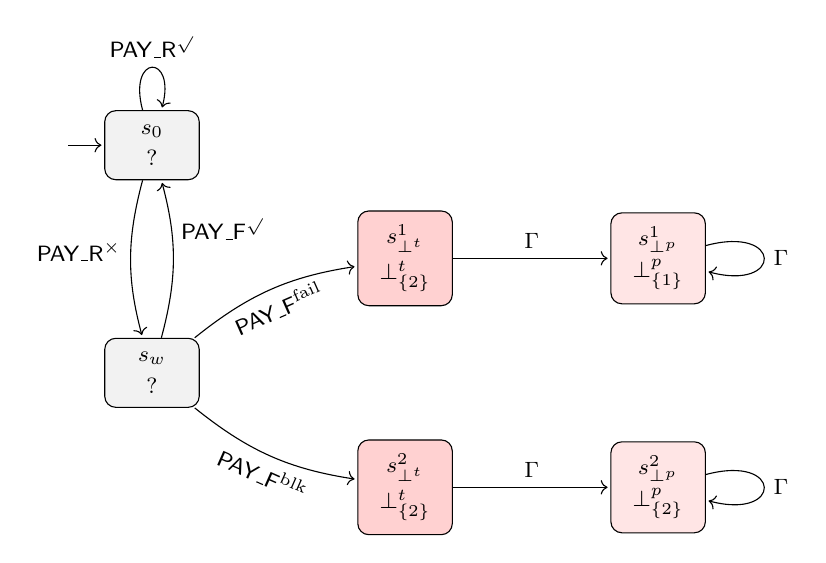
\begin{tikzpicture}[
        ->, shorten >=1pt,node distance=20mm and 20mm,
        every state/.style={
          rectangle,rounded corners,draw,
          minimum width=12mm,minimum height=7mm,
          inner sep=5pt,font=\footnotesize,align=center
        },
        initial text={}
      ]
      
      % --- Active States ---
      \node[initial,state,fill=gray!10]          (q0)  {$s_0$\\[2pt]$\mathsf{?}$};
      \node[state,fill=gray!10,below=of q0]      (qw)  {$s_w$\\[2pt]$\mathsf{?}$};
      
      % --- Split Violation States ---
      
      % Path 1: Tenant Blame (Most common case)
      \node[state,fill=red!18,above right= 4 mm and 20mm of qw]       (qv1)  {$s_{\bott}^1$\\[2pt]$\bottp{\{2\}}$};
      \node[state,fill=red!10,right=20mm of qv1]       (qpv1) {$s_{\botp}^1$\\[2pt]$\botpp{\{1\}}$};
      
      % Path 2: Landlord Blame (Blocking the fine)
      \node[state,fill=red!18,below right= 4 mm and 20mm of qw]       (qv2)  {$s_{\bott}^2$\\[2pt]$\bottp{\{2\}}$};
      \node[state,fill=red!10,right=20mm of qv2]       (qpv2) {$s_{\botp}^2$\\[2pt]$\botpp{\{2\}}$};
      
      % --- Transitions ---
      
      % 1. In-cycle behavior
      \path
          (q0) edge[loop above] node[above,pos=0.5] {\footnotesize $\PAY^\surd$} ()
          (q0) edge[bend right=15] node[left,pos=0.45] {\footnotesize $\PAY^\times$} (qw)
          (qw) edge[bend right=15] node[right,pos=0.7] {\footnotesize $\PAYF^\surd$} (q0); % Restart on repair
      
      % 2. Violation: Tenant Fault
      % Tenant fails to pay the fine (no blocking)
      \path
          (qw) edge[bend left=15] node[below,sloped] {\footnotesize $\PAYF^{\text{fail}}$} (qv1);
      
      % 3. Violation: Landlord Fault
      % Tenant attempts fine, Landlord blocks
      \path
          (qw) edge[bend right=15] node[below,sloped] {\footnotesize $\PAYF^{\text{blk}}$} (qv2);
      
      % 4. Sinks (The Limitation)
      % Once in a sink, the monitor loops forever, ignoring future events
      \path
          (qv1)  edge node[above] {\footnotesize$\Gamma$} (qpv1)
          (qpv1) edge[loop right] node {\footnotesize$\Gamma$} ()
          (qv2)  edge node[above] {\footnotesize$\Gamma$} (qpv2)
          (qpv2) edge[loop right] node {\footnotesize$\Gamma$} ();
      
      \end{tikzpicture}
      \caption{Blame Monitor for $\repit{C_3}$.
      \textbf{Limitation:} If the trace reaches $s_{\botp}^1$ (Tenant blame), the monitor remains there forever. Even if the landlord subsequently blocks a valid payment attempt ($\PAYF^{\text{blk}}$) in a future step, the verdict remains $\botpp{1}$.}
      \label{fig:rep-c3_blame}
      \end{figure}
      \end{example}     
      
\subsection{Conclusion and Limitation}      
      We have presented forward-looking semantics and a corresponding monitor construction that refine the standard satisfaction verdicts by assigning responsibility. 
      This approach is computationally efficient and provides immediate feedback on the \emph{status} of the contract, allowing for runtime enforcement and dispute resolution at the moment a breach occurs.
      
      However, this prefix-based view naturally implies a limitation regarding the completeness of the violation history. 
      The semantics is designed to detect the \emph{first} decisive violation that renders the contract permanently unsatisfiable. 
      Once the monitor transitions to a post-violation sink state ($\botpp{S}$), the verdict becomes immutable. 
      A practical consequence of this property is that, even when processing infinite words or streams, the monitor can be programmed to halt execution immediately after the first tight violation is detected, as no future event can alter the blame assignment.
      Consequently, any subsequent violations committed by other agents at later time steps are effectively masked by the first failure.
      
      This limitation is particularly evident in open-ended contracts involving the repetition operator. 
      As illustrated by the monitor for $\repit{C_3}$ (\ref{fig:rep-c3_blame}), if the tenant is blamed for failing to pay the reparation in one cycle, the monitor enters the sink state $s_{\botp}^1$. 
      Even if the interaction continues and the landlord subsequently violates their permission or obligation in a future cycle (e.g., by blocking a valid payment attempt), the monitor remains fixed on the initial verdict $\botpp{1}$. 
      Therefore, while this framework is sufficient for determining \emph{why} a contract failed, it does not support a cumulative accounting of \emph{all} violations that occur throughout the lifespan of a long-running interaction. 
      This is a notable constraint, as in law and normative systems, one typically has to account for all violations to determine the full extent of liability or penalties.
      Capturing such multi-point violations would require a mechanism to reset or parallelize monitoring threads after a failure, rather than absorbing them into a permanent sink.
      
      Finally, extending this framework to support a cumulative blame semantics suggests interesting theoretical challenges. 
      In particular, the interaction between timed operators and conjunctions complicates fault aggregation. 
      For instance, determining whether overlapping failures in concurrent branches or repeated violations within sliding time windows should be counted as distinct or continuous breaches requires a more complex, possibly non-monotonic, judgement structure than the one presented here.     

% \begin{theorem}[Correctness of the blame monitor]
% \label{thm:bm-correct}
% Let $C$ be a contract in \cDL, and let $\bmc(C)$ be its blame monitor. For
% every finite trace $\pi$ and every prefix index $k<|\pi|$, if the run of
% $\bmc(C)$ on $\pi$ is
% \[
% q_0,q_1,\dots,q_k,
% \]
% then
% \[
% \lambda_{11}(q_k) = \mathsf{Blame}_C\big(\pi[1,k]\big).
% \]
% In particular:
% \begin{itemize}
%   \item $\lambda_{11}(q_k)\in\{\mathsf{?},\topt,\topp\}$
%         iff $\pi[1,k]\in\{\presat,\satt,\postsat\}$ for $C$,
%   \item $\lambda_{11}(q_k)=\bot^t_S$
%         iff $\pi[1,k]\ \vDash_{\bottp{S}} C$,
%   \item $\lambda_{11}(q_k)=\bot^p_S$
%         iff $\pi[1,k]\ \vDash_{\botpp{S}} C$.
% \end{itemize}
% \end{theorem}

% \begin{proof}[Proof sketch]
% Correctness of the tight monitor construction $\tsmc(C)$ with respect to the
% five-valued semantics has already been established for all constructors.
% The blame rules for literals and contract operators are defined by structural
% recursion on $C$ and share the same tight frontiers as the underlying
% violation semantics. By Lemma~\ref{lem:mutual prefix}, each prefix carries at
% most one tight frontier, and the five regions are disjoint. The inductive
% clauses for blame propagation mirror the violation clauses, so for every
% reachable state $q_k$ on the run over $\pi$, the contract semantics assigns a
% unique verdict in $\mathbb{V}_{11}$ to the prefix $\pi[1,k]$.
% By Definition~\ref{def:bm-refinement}, $\lambda_{11}(q_k)$ is exactly that
% verdict. The statement follows by induction on the structure of $C$ and on the
% length of $\pi$.
% \end{proof}

% The blame monitor thus provides a concrete, prefix-based implementation of the
% forward-looking blame semantics. It reads the same synchronous trace as the
% tight satisfaction monitor, but instead of only declaring whether $C$ is
% satisfied or violated, it refines every violation region with a precise
% allocation of responsibility to the involved agents.

% \begin{example}[Blame monitors for $C_3$ and $C_2\wedge C_3$]
% We illustrate the reuse of the tight monitor construction on the rent contract
% $C_3 = \obl[1]{\PAY}\repair\obl[1]{\PAYF}$ and its conjunction with the
% permission $C_2=\perm[1]{\OCC}$.
% The five-valued monitors for $\repit{C_3}$ and for $C_2\wedge C_3$ were given
% in Example~\ref{ex:moore-c3-literals}.
% The corresponding blame monitors are obtained by keeping the same states and
% transitions and only refining the outputs.

% \begin{figure}[h!]
% \centering
% \tikzset{
%   ->, >=Stealth, semithick,
%   node distance=17mm,
%   every state/.style={
%     rectangle,rounded corners,draw,
%     minimum width=12mm,minimum height=7mm,
%     inner sep=2pt,font=\scriptsize,align=center}
% }

% % Blame monitor for rep(C3)
% \begin{subfigure}[t]{0.46\textwidth}
% \centering
% \begin{tikzpicture}
%   \node[initial,state,fill=gray!10]          (q0)  {$q_0$\\$\mathsf{?}$};
%   \node[state,fill=gray!10,below=of q0]      (qw)  {$q_w$\\$\mathsf{?}$};
%   \node[state,fill=red!18,right=of qw]       (qv)  {$q_{\bot^t}$\\$\bot^t_{\{1\}}$};
%   \node[state,fill=red!10,above=of qv]       (qpv) {$q_{\bot^p}$\\$\bot^p_{\{1\}}$};

%   \path
%     (q0) edge[loop above] node[above,pos=0.5] {\scriptsize $\PAY^\surd$} ()
%     (q0) edge[bend right=13] node[left,pos=0.45] {\scriptsize $\PAY^\times$} (qw)
%     (qw)  edge[bend right=13] node[right,pos=0.45] {\scriptsize $\PAYF^\surd$} (q0)
%     (qw)  edge[bend right=10] node[below,pos=0.45] {\scriptsize $\PAYF^\times$} (qv)
%     (qv)  edge node[left] {\footnotesize$\Gamma$} (qpv)
%     (qpv) edge[loop right] node {\footnotesize$\Gamma$} ();
% \end{tikzpicture}
% \caption{Blame monitor for $\repit{C_3}$. All unrepaired violations of $C_3$ are blamed on agent 1.}
% \label{fig:rep-c3-blame}
% \end{subfigure}
% \hfill

% % Blame monitor for C2 ^ C3
% \begin{subfigure}[t]{0.46\textwidth}
% \centering
% \scalebox{0.9}{
% \begin{tikzpicture}[
%   ->, >=Stealth, node distance=20mm and 18mm,
%   every state/.style={
%     rectangle,rounded corners,draw,
%     minimum width=12mm,minimum height=7mm,
%     inner sep=2pt,font=\scriptsize,align=center
%   }
% ]
% \node[initial,state,fill=gray!10] (q0) {$s_0$\\$\mathsf{?}$};
% \node[state, fill=gray!10, below right=16mm and 17mm of q0] (q1) {$s_1$\\$\mathsf{?}$};
% \node[state,fill=green!18,right=22mm of q0] (qs) {$s_{\topt}$\\$\topt$};
% \node[state,fill=red!18,below=28mm of q0] (qv) {$s_{\bot^t}$\\$\bot^t_{S}$};
% \node[state,fill=green!10,right=22mm of qs] (qps) {$s_{\topp}$\\$\topp$};
% \node[state,fill=red!10,below=28mm of qps] (qpv) {$s_{\bot^p}$\\$\bot^p_{S}$};

% \path[->]
%   (q0) edge[bend left=10] node[above,pos=0.5] {\scriptsize$\OCC^\surd \land \PAY^{\surd}$} (qs)
%   (q0) edge[bend right=14] node[left,pos=0.5] {\scriptsize$\OCC^{\times}$} (qv)
%   (q0) edge[bend left=12] node[pos=0.45,sloped,above] {\scriptsize$\OCC^\surd \land \PAY^{\times}$} (q1)
%   (q1) edge[bend left=8] node[right] {\scriptsize$\PAYF^\surd$} (qs)
%   (q1) edge[bend left=10] node[above,pos=0.7] {\scriptsize$\PAYF^{\times}$} (qv)
%   (qs) edge node[above] {\footnotesize$\Gamma$} (qps)
%   (qv) edge node[below] {\footnotesize$\Gamma$} (qpv)
%   (qps) edge[loop right] node {\footnotesize$\Gamma$} ()
%   (qpv) edge[loop right] node {\footnotesize$\Gamma$} ();
% \end{tikzpicture}}
% \caption{Blame monitor for $C_2\wedge C_3$. $S$ denotes the blame set prescribed by the conjunction blame rules.}
% \label{fig:c2andc3-blame}
% \end{subfigure}

% \caption{Blame monitor construction by reuse of the tight monitors for $\repit{C_3}$ and $C_2\wedge C_3$. States and transitions are inherited from the five-valued monitors; only the outputs are refined from $\bott,\botp$ to the responsibility-aware verdicts $\bot^t_S,\bot^p_S$.}
% \label{fig:blame-monitors-c2-c3}
% \end{figure}
% \end{example

\section{Quantitative Violation Semantics}

\subsection{Motivation and Scope}

\paragraph{Beyond Binary Verdicts.}
The fundamental limitation of the forward-looking tight satisfaction semantics, as defined in the previous section, lies in its binary and prefix-closed nature.
In that framework, the monitoring process halts definitively at the first tight violation.
While computationally efficient for stopping enforcement mechanisms (e.g., access control), this ``first-fail'' approach is insufficient for post-hoc auditing or dispute resolution.
It masks the full history of non-compliance, failing to capture cumulative violations or distinct failures by multiple agents over time—a critical requirement for comprehensive legal accountability.
To address this, we must transition from a boolean verdict to a \emph{quantitative semantics}, moving from the question ``Did a violation occur?'' to ``How many violations occurred, and of what magnitude?''


\paragraph{The Challenge of Temporal Scope.}
A prerequisite for counting violations is defining the temporal window over which the contract is evaluated.
Unlike traditional model checking where traces are often infinite, contract monitoring operates on finite, evolving prefixes.
We identify two primary strategies for defining this scope:

\begin{enumerate}
    \item \textbf{Static Pre-computation:} One might attempt to calculate a fixed duration $T$ for a contract $C$.
    However, contracts containing unbounded repetitions ($\repit{C}$) or input-dependent regular expressions (guards/triggers) do not have a statically determinable length.
   
    \item \textbf{Dynamic On-the-Fly Detection:} The alternative is to determine the contract's status dynamically at every step.
    Here, the monitor continuously computes a \emph{residual contract}—a formula representing what remains to be fulfilled given the history of events.
   
\end{enumerate}

In this work, we adopt the \textbf{Dynamic On-the-Fly} approach.
This requires a structural tracking mechanism, which we formalize as the \emph{Contract Progress Monitor} (CPM).
The CPM acts as a derivative function: given a contract $C$ and an incoming event, it computes the contract $C'$ that must be enforced in the next time step.
By isolating the \emph{state} of the contract (via the CPM) from the \emph{evaluation} of compliance (via a scoring function), we enable a modular framework that can track active duties, handle contrary-to-duty (CTD) transitions, and attribute blame precisely over time.


\subsection{Contract Progress Monitor}

The core of our quantitative framework is the \emph{progression function}, $\Prog$.
Conceptually similar to the Brzozowski derivative~\cite{brzozowski1964derivatives} for regular expressions, $\Prog$ consumes the current event and the current contract to produce the \emph{residual contract} for the subsequent step.

\begin{definition}[Contract Progression Function]
Let $\Gamma = 2^\Sigma$ be the event alphabet.
We extend the set of contracts $\mathcal{C}$ with a distinguished symbol $\emptc$, representing a \emph{discharged contract} (one that implies no further obligations).

The progression function $\Prog: \Gamma^* \times \cDL \to \cDL \cup \{\emptc\}$ is defined recursively.
For the empty trace $\epsilon$, $\Prog(\epsilon, C) := C$.
For a single event step $\trace{A}$ with $A \in \Gamma$, the function is defined on the structure of $C$ as follows.

\paragraph{Literals (State Update).}
For any literal $\ell$ (obligation, permission, or prohibition):
\[
\Prog(\trace{A}, \ell) := \emptc
\]
\emph{Rationale:} Structurally, a literal applies to a single time step.
Once that step $A$ occurs, the literal is consumed.
Whether $A$ satisfied or violated $\ell$ is immaterial to the \emph{progression} (the duty is passed); the violation is recorded separately by the quantitative scoring function defined later.


\paragraph{Conjunction (Parallel Progress).}
\[
\Prog(\trace{A}, C_1 \wedge C_2) := \Prog(\trace{A}, C_1) \wedge \Prog(\trace{A}, C_2)
\]
We assume the algebraic identity where $\emptc$ is the neutral element for conjunction: $\emptc \wedge C' \equiv C'$.


\paragraph{Sequence (Sequential Handover).}
For a sequence $C_1 ; C_2$, progression determines if the current step concludes $C_1$:
\[
\Prog(\trace{A}, C_1 ; C_2) := 
\begin{cases}
  \Prog(\trace{A}, C_1) ; C_2 & \text{if } \Prog(\trace{A}, C_1) \neq \emptc, \\
  \Prog(\trace{A}, C_2) & \text{if } \Prog(\trace{A}, C_1) = \emptc.
\end{cases}
\]
If $C_1$ is discharged by step $A$ (i.e., its residual is $\emptc$), the monitor immediately activates the first step of the continuation $C_2$.


\paragraph{Reparation (Contrary-to-Duty Branching).}
The reparation construct is unique because its structural evolution depends on the satisfaction of the primary obligation.
This is the only case where $\Prog$ relies on the tight satisfaction relation ($\satt, \violt, \presat$) to determine the path:
\[
\Prog(\trace{A}, C_1 \repair C_2) := 
\begin{cases}
  \Prog(\trace{A}, C_1) \repair C_2 & \text{if } \trace{A} \presat C_1 \text{ (Pending)}, \\
  \Prog(\trace{A}, C_2) & \text{if } \trace{A} \violt C_1 \text{ (Violation $\to$ Repair)}, \\
  \emptc & \text{if } \trace{A} \satt C_1 \text{ (Satisfaction $\to$ Discharge)}.
\end{cases}
\]
If a violation occurs ($\trace{A} \violt C_1$), the primary contract is discarded, and the secondary contract $C_2$ is activated immediately for the \emph{next} step.


\paragraph{Repetition.}
Repetition unrolls the contract one step at a time:
\[
\Prog(\trace{A}, \repit{C}) := \Prog(\trace{A}, C) ; \repit{C}
\]


\paragraph{Guarded and Triggered Contracts.}
These constructs rely on regular expression matching.
\[
\Prog(\trace{A}, \guard[re]{C}) :=
\begin{cases}
  \emptc & \text{if } \trace{A} \satt \guard[re]{C} \text{ (Guard satisfies, release)}, \\
  \guard[\Prog_{re}(\trace{A}, re)]{\Prog(\trace{A}, C)} & \text{otherwise (Guard persists)}.
\end{cases}
\]
\[
\Prog(\trace{A}, \trig[re]{C}) :=
\begin{cases}
  \emptc & \text{if } \trace{A} \violt re \text{ (Trigger failed permanently)}, \\
  C & \text{if } \trace{A} \satt re \text{ (Trigger fires)}, \\
  \trig[\Prog_{re}(\trace{A}, re)]{C} & \text{if } \trace{A} \presat re \text{ (Trigger pending)}.
\end{cases}
\]


\paragraph{Regular Expression Derivatives ($\Prog_{re}$).}
The helper function $\Prog_{re}$ computes the standard derivative~\cite{brzozowski1964derivatives} of the regular expression.
For atomic sets $A'$ and step $A$, $\Prog_{re}(\trace{A}, A') = \epsilon$ if matches, else failure.
For operations like union ($\mid$) and Kleene plus ($^+$), the derivatives follow standard automata-theoretic constructions.


\end{definition}

\begin{lemma}[Termination]
For any finite prefix $\pi$, $\Prog(\pi, C)$ terminates in at most $|\pi|$ recursive steps.

\end{lemma}
To illustrate the CPM, we examine how the residual contract evolves under different traces. We begin with the fundamental building block of normative enforcement: the reparation.

\begin{example}[Progression of Reparation]
\label{ex:prog-repit}
Consider the basic rental reparation clause:
\[ C_3 := \obl[1]{\PAY}\ \repair\ \obl[1]{\PAYF}. \]

\noindent\textbf{Scenario 1: Compliance.}
In the first trace $\pi$, the tenant pays rent in Month 1 ($\PAY \in A_1$). Since $\trace{A_1} \satt \obl[1]{\PAY}$, the condition for discharge is met. The reparation structure collapses to $\emptc$, meaning no further obligations exist for Month 2.

    \boxalignfigure{\resizebox{0.7\textwidth}{!}{%
    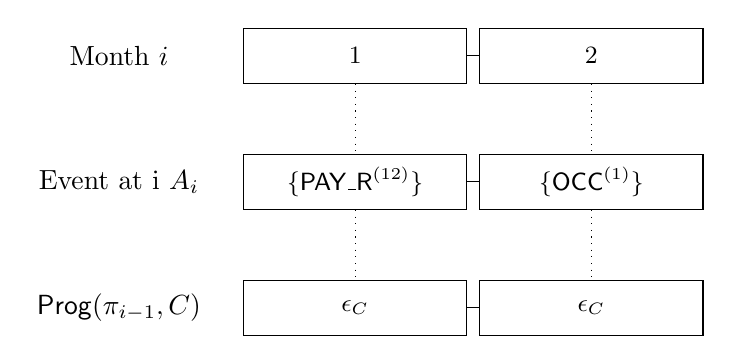
\begin{tikzpicture}[y=1.6cm,x=3.0cm]
    
      \tikzset{
        cell/.style={
          draw, rectangle, text width=26mm,
          minimum height=7mm, align=center, font=\small
        }
      }
    
      % Labels
      \node at (0,0)   {Month $i$};
      \node at (0,-1)  {Event at i $A_i$};
      \node at (0,-2)  {$\Prog(\pi_{i-1},C)$};
      % Row 1: time
      \node[cell] at (1,0) (t1) {$1$};
      \node[cell] at (2,0) (t2) {$2$};
      % Row 2: events
      \node[cell] at (1,-1) (e1) {$\{\PAY^{(12)}\}$};
      \node[cell] at (2,-1) (e2) {$\{\OCC^{(1)}\}$};
      % Row 3: residuals
      \node[cell] at (1,-2) (r1) {\emptc};
      \node[cell] at (2,-2) (r2) {\emptc};
      % Arrows
      \draw (t1)--(t2);
      \draw (e1)--(e2);
      \draw (r1)--(r2);
      % Vertical alignment
      \draw[dotted](t1.south)--(e1.north);
      \draw[dotted](e1.south)--(r1.north);
    
      \draw[dotted](t2.south)--(e2.north);
      \draw[dotted](e2.south)--(r2.north);
    \end{tikzpicture}
    }}
    {Progression on $ \obl[1]{\PAY}\ \repair\ \obl[1]{\PAYF}$ with a trace for which a no reparation is not required}
    {example:prog-repair1}
    {\vspace{8pt}}{\vspace{-12pt}}

\medskip
\noindent\textbf{Scenario 2: Violation and Repair.}
In trace $\pi'$, the tenant fails to pay in Month 1 ($\PAY \notin A'_1$). Here, $\trace{A'_1} \violt \obl[1]{\PAY}$. Consequently, the CPM activates the repair branch. The residual for Month 2 becomes $\obl[1]{\PAYF}$, obliging the tenant to pay the fine.

  \boxalignfigure{\resizebox{0.7\textwidth}{!}{%
  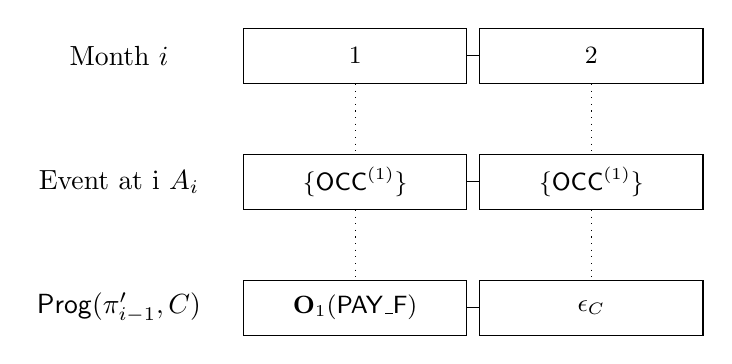
\begin{tikzpicture}[y=1.6cm,x=3.0cm]
  
    \tikzset{
      cell/.style={
        draw, rectangle, text width=26mm,
        minimum height=7mm, align=center, font=\small
      }
    }
  
    % Labels
    \node at (0,0)   {Month $i$};
    \node at (0,-1)  {Event at i $A_i$};
    \node at (0,-2)  {$\Prog(\pi'_{i-1},C)$};
    % Row 1: time
    \node[cell] at (1,0) (t1) {$1$};
    \node[cell] at (2,0) (t2) {$2$};
    % Row 2: events
    \node[cell] at (1,-1) (e1) {$\{\OCC^{(1)}\}$};
    \node[cell] at (2,-1) (e2) {$\{\OCC^{(1)}\}$};
    % Row 3: residuals
    \node[cell] at (1,-2) (r1) {$\obl[1]{\PAYF}$};
    \node[cell] at (2,-2) (r2) {\emptc};
    % Arrows
    \draw (t1)--(t2);
    \draw (e1)--(e2);
    \draw (r1)--(r2);
  
    % Vertical alignment
    \draw[dotted](t1.south)--(e1.north);
    \draw[dotted](e1.south)--(r1.north);
  
    \draw[dotted](t2.south)--(e2.north);
    \draw[dotted](e2.south)--(r2.north);
  
  \end{tikzpicture}
  }}
  {Progression on $ \obl[1]{\PAY}\ \repair\ \obl[1]{\PAYF}$ with a trace for which a no reparation is not required}
  {example:prog-repair2}
  {\vspace{8pt}}{\vspace{-12pt}}
\end{example}

Having established how single-step reparations evolve, we now extend the analysis to ongoing contracts. The following example demonstrates how the CPM handles infinite streams where duties recur every month, showing how violations in one period persist into the next.

\begin{example}[Progression of Infinite Repetition]
Consider the recurring contract $\repit{C_3}$, where the tenant must pay rent (or a fine) every month.
\[ \repit{C_3} = \repit{ \obl[1]{\PAY}\ \repair\ \obl[1]{\PAYF}}. \]

\noindent\textbf{Trace Analysis.}
We observe a trace where the tenant pays in Month 1 but fails to pay in Month 2 (occupying instead).
\begin{itemize}
    \item \textbf{Step 1 ($A_1$):} The tenant pays. The instance of $C_3$ for Month 1 is discharged. Due to the repetition operator, the residual is $\emptc ; \repit{C_3} \equiv \repit{C_3}$. The contract effectively ``resets'' for the next month.
    \item \textbf{Step 2 ($A_2$):} The tenant occupies but does not pay. The instance of $C_3$ for Month 2 is violated. Unlike Step 1, the residual does not reset cleanly. Instead, the violated obligation transforms into its reparation $\obl[1]{\PAYF}$, which must be fulfilled in the \emph{next} step (Month 3), alongside the continuing repetition $\repit{C_3}$.
\end{itemize}
This results in an accumulation of duties: the fine from Month 2 and the new rent for Month 3.

  \boxalignfigure{\resizebox{0.7\textwidth}{!}{%
  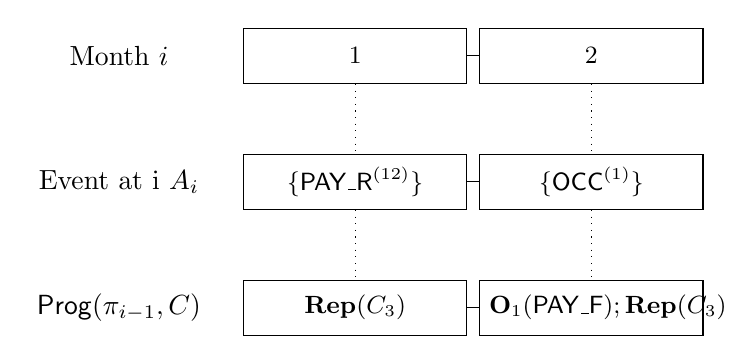
\begin{tikzpicture}[y=1.6cm,x=3.0cm]
  
    \tikzset{
      cell/.style={
        draw, rectangle, text width=26mm,
        minimum height=7mm, align=center, font=\small
      }
    }
  
    % Labels
    \node at (0,0)   {Month $i$};
    \node at (0,-1)  {Event at i $A_i$};
    \node at (0,-2)  {$\Prog(\pi_{i-1},C)$};
    % Row 1: time
    \node[cell] at (1,0) (t1) {$1$};
    \node[cell] at (2,0) (t2) {$2$};
    % Row 2: events
    \node[cell] at (1,-1) (e1) {$\{\PAY^{(12)}\}$};
    \node[cell] at (2,-1) (e2) {$\{\OCC^{(1)}\}$};
    % Row 3: residuals
    \node[cell] at (1,-2) (r1) {$\repit{C_3}$};
    \node[cell] at (2,-2) (r2) {$\obl[1]{\PAYF} ; \repit{C_3}$};
    % Arrows
    \draw (t1)--(t2);
    \draw (e1)--(e2);
    \draw (r1)--(r2);
  
    % Vertical alignment
    \draw[dotted](t1.south)--(e1.north);
    \draw[dotted](e1.south)--(r1.north);
  
    \draw[dotted](t2.south)--(e2.north);
    \draw[dotted](e2.south)--(r2.north);
  
  \end{tikzpicture}
  }}
  {Progression on $\repit{C_3}$ where the obligation is met in the first month but violated in the second.}
  {example:prog-repitc1}
  {\vspace{8pt}}{\vspace{-12pt}}
\end{example}

While repetitions capture simple recurring duties, more complex contracts are often bounded by conditions. Finally, we examine how the CPM handles \emph{guarded contracts}, where the outer structure (the guard) and the inner structure (the obligations) evolve independently until a termination event occurs.

\begin{example}[Progression of Guarded Contracts]
We examine a guarded contract that persists until a termination notice ($\notifterm$) is issued.
\[ \guard[\Gamma^+ \cdot \notifterm^{(1)}]{\repit{C_3}} \]

\noindent\textbf{Trace 1: Successful Termination.}
The tenant pays in Month 1 ($A_1$) and issues a termination notice in Month 2 ($A_2$).
\begin{itemize}
    \item At $i=1$, the event $A_1$ satisfies the inner contract $C_3$ (rent paid), but does not satisfy the guard (no notice). The residual is the guarded repetition.
    \item At $i=2$, the event $A_2$ contains $\notifterm$. This satisfies the guard expression. The CPM immediately reduces the entire contract to $\emptc$, signifying the contract has ended.
\end{itemize}

  \boxalignfigure{\resizebox{0.85\textwidth}{!}{%
  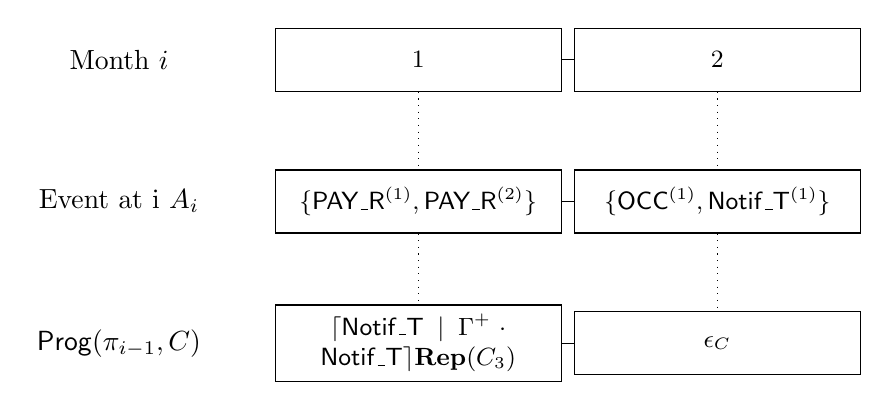
\begin{tikzpicture}[y=1.8cm,x=3.8cm]
  
    \tikzset{
      cell/.style={
        draw, rectangle, text width=34mm,
        minimum height=8mm, align=center, font=\small
      }
    }
    % Local definition for the residual regex to fit in the box
    \def\resid{\notifterm \mid \Gamma^+ \cdot \notifterm}
  
    % Labels
    \node at (0,0)   {Month $i$};
    \node at (0,-1)  {Event at i $A_i$};
    \node at (0,-2)  {$\Prog(\pi_{i-1},C)$};
    % Row 1: time
    \node[cell] at (1,0) (t1) {$1$};
    \node[cell] at (2,0) (t2) {$2$};
    % Row 2: events
    \node[cell] at (1,-1) (e1) {$\{\PAY^{(1)}, \PAY^{(2)}\}$};
    \node[cell] at (2,-1) (e2) {$\{\OCC^{(1)}, \notifterm^{(1)}\}$};
    % Row 3: residuals
    % Step 1: Contract satisfied (payment made), Guard not satisfied yet (needs >0 length or specific event).
    % Residual guard becomes (Notif | Gamma+ . Notif)
    \node[cell] at (1,-2) (r1) {$\guard[\resid]{\repit{C_3}}$};
    % Step 2: Guard satisfied by NotifTerm in A2. Contract discharges to epsilon.
    \node[cell] at (2,-2) (r2) {\emptc};
    % Arrows
    \draw (t1)--(t2);
    \draw (e1)--(e2);
    \draw (r1)--(r2);
  
    % Vertical alignment
    \draw[dotted](t1.south)--(e1.north);
    \draw[dotted](e1.south)--(r1.north);
  
    \draw[dotted](t2.south)--(e2.north);
    \draw[dotted](e2.south)--(r2.north);
  
  \end{tikzpicture}
  }}
  {Progression on guarded contract where the termination notice at step 2 discharges the contract.}
  {example:prog-guard1}
  {\vspace{8pt}}{\vspace{-12pt}}

\medskip
\noindent\textbf{Trace 2: Pending Guard with Internal Violation.}
In this scenario, the tenant pays in Month 1 but fails to pay (and gives no notice) in Month 2.
\begin{itemize}
    \item At $i=2$, the guard is \emph{not} satisfied.
    \item Simultaneously, the inner contract $\repit{C_3}$ processes the event. Since rent was not paid, the inner contract evolves into a reparation state ($\obl[1]{\PAYF}$).
    \item The resulting residual is a guarded reparation: $\guard[\dots]{(\obl[1]{\PAYF} ; \repit{C_3})}$.
\end{itemize}
This illustrates how the CPM maintains the ``wrapper'' (the guard) while the content inside (the obligations) evolves and accumulates violations independently.

  \boxalignfigure{\resizebox{0.95\textwidth}{!}{%
  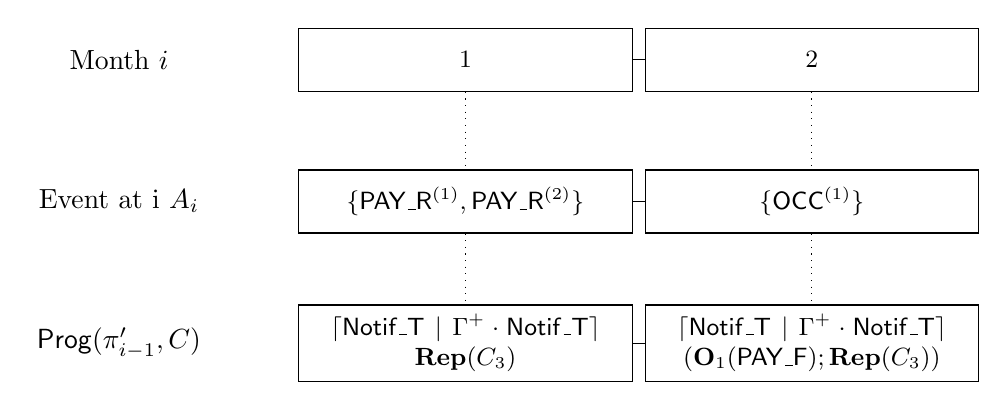
\begin{tikzpicture}[y=1.8cm,x=4.4cm]
  
    \tikzset{
      cell/.style={
        draw, rectangle, text width=40mm,
        minimum height=8mm, align=center, font=\small
      }
    }
    \def\resid{\notifterm \mid \Gamma^+ \cdot \notifterm}
  
    % Labels
    \node at (0,0)   {Month $i$};
    \node at (0,-1)  {Event at i $A_i$};
    \node at (0,-2)  {$\Prog(\pi'_{i-1},C)$};
    
    % Row 1: time
    \node[cell] at (1,0) (t1) {$1$};
    \node[cell] at (2,0) (t2) {$2$};
    
    % Row 2: events
    \node[cell] at (1,-1) (e1) {$\{\PAY^{(1)}, \PAY^{(2)}\}$};
    \node[cell] at (2,-1) (e2) {$\{\OCC^{(1)}\}$};
    
    % Row 3: residuals
    % Step 1: Manual line break using \\
    \node[cell] at (1,-2) (r1) {$\lceil \resid \rceil$ \\ $\repit{C_3}$};
    % Step 2: Manual line break using \\
    \node[cell] at (2,-2) (r2) {$\lceil \resid \rceil$ \\ $(\obl[1]{\PAYF} ; \repit{C_3})$};
    % Arrows
    \draw (t1)--(t2);
    \draw (e1)--(e2);
    \draw (r1)--(r2);
  
    % Vertical alignment
    \draw[dotted](t1.south)--(e1.north);
    \draw[dotted](e1.south)--(r1.north);
  
    \draw[dotted](t2.south)--(e2.north);
    \draw[dotted](e2.south)--(r2.north);
  
  \end{tikzpicture}
  }}
  {Progression on guarded contract where the guard is not satisfied and the inner contract triggers a reparation.}
  {example:prog-guard2}
  {\vspace{8pt}}{\vspace{-12pt}}
  
\end{example}


\section{Quantative violation semantics}
To define the quantitative violation semantics to not stop at the first violation prefix, we reuse  \emph{Contract Progress function} as the underlying state-transition mechanism.
 The progression function $\Prog$ is utilized to dynamically evolve the contract after every observation, producing a sequence of \emph{residual contracts} that represent the exact normative state at each point in time.
  By updating the contract state step-by-step, we ensure that the violation score for any given event is calculated strictly against the specific literals in force at that moment, accounting for all prior satisfactions, discharges, or triggered reparations. Then propagating the updated residual to the subsequent evaluation step.
  \begin{definition}[Quantitative Violation Semantics]
    Let $\trace{A}$ be a single event trace over $\Gamma$,  $\pi$ be a (possibly empty) finite trace $\Gamma^*$, and $C$ be a contract from $\cDL$.
    We define the \emph{quantitative violation semantics}, denoted by $\qsem{}: \Gamma^*, \cDL \to \mathbb{N} $, which maps a trace and a contract to a  natural number representing the violation score of trace on the contract. 
    The function is defined recursively by evaluating the head of the trace ($\trace{A}$) and propagating the residual contract to the tail ($\pi$):
    \[
    \qsem{\trace{A}\concat \pi, C} :=
    \begin{cases} 
      \qsem{\trace{A}, C } & \text{if } \pi = \epsilon \lor \Prog(\trace{A},C)= \emptc,\\
      \qsem{\trace{A}, C } + \qsem{\pi, \Prog(\trace{A},C)} & \text{otherwise}.
    \end{cases}
    \]
    where the \emph{instantaneous violation score} for a single event $\trace{A}$ against a contract $C$ is defined inductively on the structure of the contract:
    \[
    \qsem{\trace{A}, C} :=
    \begin{cases} 
      \qsem{\trace{A}, C_1 } + \qsem{\trace{A}, C_2} & \text{if } C = C_1 \wedge C_2, \\
      1 & \text{if } \trace{A} \violt C, \\
      0 & \text{otherwise}.
    \end{cases}
    \]
    \end{definition}
Intuitively, the formula $\qsem{\trace{A}\concat \pi, C}$ treats the contract execution as a path-accumulation problem. At every time step, the function:
\begin{enumerate}
    \item \textbf{Snapshots the penalty:} It calculates $\qsem{\trace{A}, C}$, which asks ``Given the current literals from$C$, does the current event $A$ violate any of them?'' This is a stateless check based purely on the structure of $C$ at that instant.
    \item \textbf{Updates the state:} It computes $\Prog(\trace{A}, C)$, effectively moving the contract pointer forward (e.g., from a paid obligation to the next month's rent, or from a violated duty to a reparation).
    \item \textbf{Accumulates:} It adds the snapshot penalty to the result of the recursive call on the remaining trace using the \emph{new} state.
\end{enumerate}

Intuitively, the formula $\qsem{\trace{A}\concat \pi, C}$ treats the contract execution as a path-accumulation problem. At every time step, the function:
\begin{enumerate}
    \item \textbf{Snapshots the penalty:} It calculates $\qsem{\trace{A}, C}$, which asks ``Given the current literals from $C$, does the current event $A$ violate any of them?'' This is a stateless check based purely on the structure of $C$ at that instant.
    \item \textbf{Updates the state:} It computes $\Prog(\trace{A}, C)$, effectively moving the contract pointer forward (e.g., from a paid obligation to the next month's rent, or from a violated duty to a reparation).
    \item \textbf{Accumulates:} It adds the snapshot penalty to the result of the recursive call on the remaining trace using the \emph{new} state.
\end{enumerate}

The explicit handling of Sequence and Reparation is done in the contract progress function, which ensures that ``zero-delay'' transitions are penalized correctly. For instance, if a contract requires $C_1$ then $C_2$, and an event discharges $C_1$ but violates $C_2$ in the same step, the summation logic ($\qsem{\trace{A}, C_1} + \qsem{\trace{A}, C_2}$) ensures the violation of $C_2$ is not ignored simply because it appeared in a continuation.


The definition of the instantaneous score $\qsem{\trace{A}, C}$ rests on distinguishing between \textbf{concurrent} (parallel) obligations and \textbf{structural} (atomic) constraints. It decouples the measurement of the ``volume'' of non-compliance from the binary verification of specific rules.

\paragraph{Additivity of Concurrency.}
The case $\qsem{\trace{A}, C_1 \wedge C_2} := \qsem{\trace{A}, C_1 } + \qsem{\trace{A}, C_2}$ captures the ``width'' of the violation as show in Example.\ref{fig:joint-blame}. In normative systems, a conjunction represents distinct, independent obligations active simultaneously. By summing the scores, the function ensures that the penalty is proportional to the number of distinct parallel duties neglected in a single instant, preventing ``violation masking'' where a single boolean verdict would hide multiple breaches.

\paragraph{Binary Structural Verdict.}
For constructs that are not distinct parallel duties (such as literals, sequences, or reparations), the definition relies on the binary tight violation relation ($\violt$). This captures the ``existence'' of a fault in a non-decomposable structure. For example, a single atomic duty ($\obl{a}$) can only be violated once per step.

\paragraph{Separation of State and Score.}
This approach assumes that the complexity of temporal evolution is handled by $\Prog$, while $\qsem{}$ handles the instantaneous cost. By reducing non-conjunction cases to a simple check ($\trace{A} \violt C$), the definition asserts that scoring is local (checking if the current active node is broken), while progression is temporal (handling the flow from one obligation to the next).

We summarize these properties in the following theorem, which establishes that the quantitative score is a monotonically increasing function that acts as a "super-set" of the binary violation semantics.
While a binary trace might be "Satisfied" (via reparation), the quantitative score reveals the cost of that path.

\subsection{Formal Correspondence between Tight and Quantitative Semantics}

The quantitative semantics presented above is not an arbitrary metric but a consistent extension of the forward-looking tight semantics.
While tight semantics provides a binary decisive verdict (satisfaction vs.\ violation), the quantitative semantics provides a cumulative measure of deviation.
We now establish the formal link between these two frameworks through the properties of \emph{Score Stability} and \emph{Violation Detection}.

The first connection concerns the relationship between the discharge of a contract (reaching $\emptc$) and the tight satisfaction relation $\satt$.
When a contract is tightly satisfied, it conceptually ceases to impose new requirements.
The progression function reflects this by transitioning to the neutral element $\emptc$.

\begin{lemma}[Satisfaction Saturation]
\label{lem:sat-saturation}
Let $C$ be a contract and $\pi$ be a finite trace.
If the contract is tightly satisfied by $\pi$, the progression function reduces to the empty contract, and the cumulative violation score stabilizes.
Formally:
\[
\pi \satt C \implies \Prog(\pi, C) = \emptc.
\]
Consequently, for any extension $\pi'$ of $\pi$:
\[
\qsem{\pi \concat \pi', C} = \qsem{\pi, C}.
\]
\end{lemma}

\begin{proof}
The proof follows from the definition of $\Prog$.
For every construct (Literal, Reparation, Guard, Trigger), the progression function is defined to return $\emptc$ exactly when the condition $\trace{A} \satt C$ is met.
Since $\qsem{\trace{A}, \emptc} = 0$ for any event $A$, no further penalties can be accumulated once the residual contract becomes $\emptc$.
\end{proof}

The second connection concerns the relationship between tight violations and the instantaneous score.
A key feature of the quantitative semantics is that it is strictly stricter than the binary semantics: it assigns a positive penalty to \emph{every} tight violation, even those that are subsequently repaired.

\begin{lemma}[Positive Penalty for Tight Violation]
\label{lem:violation-penalty}
Let $C$ be a contract and $\trace{A}$ be a single event.
If the event tightly violates the contract, the instantaneous violation score is strictly positive.
\[
\trace{A} \violt C \implies \qsem{\trace{A}, C} \ge 1.
\]
\end{lemma}

\begin{proof}
We proceed by structural induction on $C$.
\begin{itemize}
    \item \textbf{Base Case (Literals):} If $\trace{A} \violt \ell$, then by definition $\qsem{\trace{A}, \ell} = 1$.
    \item \textbf{Conjunction ($C_1 \wedge C_2$):} By Definition~\ref{def:binary-contract-semantics}, $\trace{A} \violt C_1 \wedge C_2$ implies $\trace{A} \violt C_1$ or $\trace{A} \violt C_2$.
    Consequently, $\qsem{\trace{A}, C_1} \ge 1$ or $\qsem{\trace{A}, C_2} \ge 1$. Since the score is additive ($\qsem{\trace{A}, C_1} + \qsem{\trace{A}, C_2}$), the total is $\ge 1$.
    \item \textbf{Reparation ($C_1 \repair C_2$):} $\trace{A} \violt C_1 \repair C_2$ implies $\trace{A} \violt C_1$ and $\trace{A} \violt C_2$.
    The scoring function sums violations of $C_1$ (score 1) and $C_2$. Thus, the score is at least 1.
\end{itemize}
The sequence case follows similarly via the immediate handover logic.
\end{proof}

We summarize these properties in the following theorem, which establishes that the quantitative score is a monotonically increasing function that acts as a "super-set" of the binary violation semantics.
While a binary trace might be "Satisfied" (via reparation), the quantitative score reveals the cost of that path.


\begin{theorem}[Consistency of Quantitative and Tight Semantics]
  \label{thm:quant-consistency}
  For any contract $C$ and finite trace $\pi$:
  \begin{enumerate}
      \item \textbf{Zero Score Implications:}
      If $\qsem{\pi, C} = 0$, then exactly one of the following three disjoint cases holds:
      \begin{enumerate}
        \item $\pi \satt C$ if and only if $\Prog(\pi, C) = \emptc$ and $\forall k < |\pi|-1:\Prog(\pi[0,k], C) \neq \emptc$.
        \item $\pi \postsat C$ if and only if $\Prog(\pi, C) = \emptc$ and\\ $\exists k < |\pi|-1$ such that $\Prog(\pi[0,k], C) = \emptc$.
        \item $\pi \presat C$ if and only if $\Prog(\pi, C) \neq \emptc$.
      \end{enumerate}
      
      \item \textbf{Non-Zero Score Implications:}
      If $\qsem{\pi, C} \neq 0$, then:
      \begin{enumerate}
        \item $\pi \violt C$ if and only if $\qsem{\pi, C} = 1$ and $\qsem{\pi[0, |\pi|-2], C} = 0$.
        \item $\pi \postviol C$ if and only if $\qsem{\pi, C} > 1$ or ($\qsem{\pi, C} = 1$ and\\ $\qsem{\pi[0, |\pi|-2], C} = 1$).
      \end{enumerate}
      
      \item \textbf{Reparation Cost:}
      If $\pi$ satisfies $C$ strictly through a reparation mechanism (i.e., $\pi \satt C$ but primary obligations failed), then $\qsem{\pi, C} > 0$.
  \end{enumerate}
  \end{theorem}
  
  \begin{proof}
  We prove the implications by structural induction on the trace $\pi$ and the contract $C$, utilizing the definitions of the quantitative function $\qsem{}$ and the contract progression $\Prog$.
  
  \paragraph{1. Zero Score Implications ($\qsem{\pi, C} = 0$)}
  Assume $\qsem{\pi, C} = 0$. By the definition of the cumulative score, this implies that for all steps $i < |\pi|$, the instantaneous penalty is zero: $\qsem(\trace{A_i}, C_i) = 0$. Consequently, no tight violation has occurred at any step. The contract state evolves purely via $\Prog$ without triggering any penalty clauses.
  
  \begin{enumerate}
      \item \textbf{Case 1(a): Tight Satisfaction ($\satt$).}
      \begin{itemize}
          \item $(\Rightarrow)$ Assume $\Prog(\pi, C) = \emptc$ and for all strict prefixes $\pi'$, $\Prog(\pi', C) \neq \emptc$.
          The condition $\Prog(\pi, C) = \emptc$ indicates that the contract has been fully discharged. Since the score is 0, this discharge was not achieved via a violation-triggered path (e.g., a reparation where the primary failed). The absence of $\emptc$ in prior prefixes ensures that this is the \emph{first} moment of discharge. By Definition~\ref{def:binary-contract-semantics} (Tight Satisfaction), the first prefix to fully satisfy the obligations corresponds to $\satt$.
          \item $(\Leftarrow)$ If $\pi \satt C$, then by Lemma~\ref{lem:sat-saturation} (Satisfaction Saturation), the progression must reach $\emptc$ exactly at $\pi$. Since it is a \emph{tight} satisfaction, no proper prefix could have satisfied it (reached $\emptc$) earlier.
      \end{itemize}
  
      \item \textbf{Case 1(b): Post Satisfaction ($\postsat$).}
      \begin{itemize}
          \item The condition $\exists k < |\pi|$ such that $\Prog(\pi[0,k], C) = \emptc$ implies that the contract was already discharged at a previous step $k$.
          \item By Definition~\ref{def:postprecont}, $\pi \postsat C$ holds if there exists a strict prefix that tightly satisfies $C$. Since the score is 0, the path to $k$ was compliant. Thus, the state remains $\emptc$ for the remainder of the trace, maintaining the $\postsat$ status.
      \end{itemize}
  
      \item \textbf{Case 1(c): Pre Satisfaction ($\presat$).}
      \begin{itemize}
          \item Assume $\Prog(\pi, C) \neq \emptc$. Since $\qsem{\pi, C} = 0$, no violation has occurred. However, the contract has not reduced to the empty contract $\emptc$, meaning active obligations remain.
          \item This satisfies the definition of $\presat$: the trace is neither satisfied ($\satt/\postsat$) nor violated ($\violt/\postviol$). It is effectively "pending."
      \end{itemize}
  \end{enumerate}
  
  \paragraph{2. Non-Zero Score Implications ($\qsem{\pi, C} \neq 0$)}
  Assume $\qsem{\pi, C} > 0$. This implies $\exists i$ such that $\qsem(\trace{A_i}, C_i) > 0$.
  
  \begin{enumerate}
      \item \textbf{Case 2(a): Tight Violation ($\violt$).}
      \begin{itemize}
          \item We consider the case where $\qsem{\pi, C} = 1$, the score of the immediate prefix is $0$ and let $n= \size{\pi}$ .
          \item $\qsem{\pi[0..n-2], C} = 0$ implies that for all previous steps, the contract was in a compliant state ($\presat$).
          \item The jump to $\qsem{\pi, C} = 1$ implies that the instantaneous score at the last step $\qsem{\trace{A_{n-1}}, \Prog(\pi[0,n-2],C)} = 1$.
          \item By Lemma~\ref{lem:violation-penalty}, a positive instantaneous score corresponds to a tight violation of the active residual contract.
          \item Since this is the \emph{first} non-zero score, it corresponds to the \emph{first} prefix that triggers a violation. This matches the definition of $\pi \violt C$.
      \end{itemize}
  
      \item \textbf{Case 2(b): Post Violation ($\postviol$).}
      \begin{itemize}
          \item The condition $\qsem{\pi, C} > 1$ or ($\qsem{\pi, C}=1$ and $\qsem{prefix}=1$) implies that the violation score did not originate purely at the current step (or if it did, it was cumulative).
          \item Specifically, if $\qsem{\pi[0..n-2], C} \ge 1$, then a violation occurred strictly in the past.
          \item By Definition~\ref{def:postprecont}, if a strict prefix tightly violated the contract ($\violt$), the current trace is in $\postviol$. The non-zero score is carried forward monotonically.
      \end{itemize}
  
      \item \textbf{Case 2(c): Reparation Cost.}
      \begin{itemize}
          \item Consider a contract $C_{primary} \repair C_{repair}$.
          \item If $\pi$ satisfies this strictly through the reparation mechanism, it means $\pi$ did \emph{not} satisfy $C_{primary}$.
          \item By the definition of reparation progression, the transition to $C_{repair}$ occurs only if $\pi \violt C_{primary}$.
          \item By the definition of the instantaneous scoring function for reparation,\\ $\qsem{\trace{A}, C_{primary} \repair C_{repair}} = 1 + \dots$ when the primary violates.
      \end{itemize}
      Therefore, the path involving the repair accumulates a score of at least 1 (the penalty for breaking the primary), confirming $\qsem{\pi, C} > 0$.
  \end{enumerate}
  \end{proof}

This theorem highlights the utility of the quantitative approach for post-hoc analysis: distinguishing between a "perfect" execution (Score 0) and a "compliant but costly" execution (Score $>0$, e.g., paying fines), a distinction lost in the binary $\satt$ verdict.

\section{Quantitative Violation Semantics}

\subsection{Motivation and Scope}

\paragraph{Beyond Binary Verdicts.}
The fundamental limitation of the forward-looking tight satisfaction semantics, as defined in the previous section, lies in its binary and prefix-closed nature.
In that framework, the monitoring process halts definitively at the first tight violation.
While computationally efficient for stopping enforcement mechanisms (e.g., access control), this ``first-fail'' approach is insufficient for post-hoc auditing or dispute resolution.
It masks the full history of non-compliance, failing to capture cumulative violations or distinct failures by multiple agents over time—a critical requirement for comprehensive legal accountability.
To address this, we must transition from a boolean verdict to a \emph{quantitative semantics}, moving from the question ``Did a violation occur?'' to ``How many violations occurred, and of what magnitude?''


\paragraph{The Challenge of Temporal Scope.}
A prerequisite for counting violations is defining the temporal window over which the contract is evaluated.
Unlike traditional model checking where traces are often infinite, contract monitoring operates on finite, evolving prefixes.
We identify two primary strategies for defining this scope:

\begin{enumerate}
    \item \textbf{Static Pre-computation:} One might attempt to calculate a fixed duration $T$ for a contract $C$.
    However, contracts containing unbounded repetitions ($\repit{C}$) or input-dependent regular expressions (guards/triggers) do not have a statically determinable length.
   
    \item \textbf{Dynamic On-the-Fly Detection:} The alternative is to determine the contract's status dynamically at every step.
    Here, the monitor continuously computes a \emph{residual contract}—a formula representing what remains to be fulfilled given the history of events.
   
\end{enumerate}

In this work, we adopt the \textbf{Dynamic On-the-Fly} approach.
This requires a structural tracking mechanism, which we formalize as the \emph{Contract Progress Monitor} (CPM).
The CPM acts as a derivative function: given a contract $C$ and an incoming event, it computes the contract $C'$ that must be enforced in the next time step.
By isolating the \emph{state} of the contract (via the CPM) from the \emph{evaluation} of compliance (via a scoring function), we enable a modular framework that can track active duties, handle contrary-to-duty (CTD) transitions, and attribute blame precisely over time.


\subsection{Contract Progress Monitor}

The core of our quantitative framework is the \emph{progression function}, $\Prog$.
Conceptually similar to the Brzozowski derivative~\cite{brzozowski1964derivatives} for regular expressions, $\Prog$ consumes the current event and the current contract to produce the \emph{residual contract} for the subsequent step.

\begin{definition}[Contract Progression Function]
Let $\Gamma = 2^\Sigma$ be the event alphabet.
We extend the set of contracts $\mathcal{C}$ with a distinguished symbol $\emptc$, representing a \emph{discharged contract} (one that implies no further obligations).

The progression function $\Prog: \Gamma^* \times \cDL \to \cDL \cup \{\emptc\}$ is defined recursively.
For the empty trace $\epsilon$, $\Prog(\epsilon, C) := C$.
For a single event step $\trace{A}$ with $A \in \Gamma$, the function is defined on the structure of $C$ as follows.

\paragraph{Literals (State Update).}
For any literal $\ell$ (obligation, permission, or prohibition):
\[
\Prog(\trace{A}, \ell) := \emptc
\]
\emph{Rationale:} Structurally, a literal applies to a single time step.
Once that step $A$ occurs, the literal is consumed.
Whether $A$ satisfied or violated $\ell$ is immaterial to the \emph{progression} (the duty is passed); the violation is recorded separately by the quantitative scoring function defined later.


\paragraph{Conjunction (Parallel Progress).}
\[
\Prog(\trace{A}, C_1 \wedge C_2) := \Prog(\trace{A}, C_1) \wedge \Prog(\trace{A}, C_2)
\]
We assume the algebraic identity where $\emptc$ is the neutral element for conjunction: $\emptc \wedge C' \equiv C'$.


\paragraph{Sequence (Sequential Handover).}
For a sequence $C_1 ; C_2$, progression determines if the current step concludes $C_1$:
\[
\Prog(\trace{A}, C_1 ; C_2) := 
\begin{cases}
  \Prog(\trace{A}, C_1) ; C_2 & \text{if } \Prog(\trace{A}, C_1) \neq \emptc, \\
  \Prog(\trace{A}, C_2) & \text{if } \Prog(\trace{A}, C_1) = \emptc.
\end{cases}
\]
If $C_1$ is discharged by step $A$ (i.e., its residual is $\emptc$), the monitor immediately activates the first step of the continuation $C_2$.


\paragraph{Reparation (Contrary-to-Duty Branching).}
The reparation construct is unique because its structural evolution depends on the satisfaction of the primary obligation.
This is the only case where $\Prog$ relies on the tight satisfaction relation ($\satt, \violt, \presat$) to determine the path:
\[
\Prog(\trace{A}, C_1 \repair C_2) := 
\begin{cases}
  \Prog(\trace{A}, C_1) \repair C_2 & \text{if } \trace{A} \presat C_1 \text{ (Pending)}, \\
  \Prog(\trace{A}, C_2) & \text{if } \trace{A} \violt C_1 \text{ (Violation $\to$ Repair)}, \\
  \emptc & \text{if } \trace{A} \satt C_1 \text{ (Satisfaction $\to$ Discharge)}.
\end{cases}
\]
If a violation occurs ($\trace{A} \violt C_1$), the primary contract is discarded, and the secondary contract $C_2$ is activated immediately for the \emph{next} step.


\paragraph{Repetition.}
Repetition unrolls the contract one step at a time:
\[
\Prog(\trace{A}, \repit{C}) := \Prog(\trace{A}, C) ; \repit{C}
\]


\paragraph{Guarded and Triggered Contracts.}
These constructs rely on regular expression matching.
\[
\Prog(\trace{A}, \guard[re]{C}) :=
\begin{cases}
  \emptc & \text{if } \trace{A} \satt \guard[re]{C} \text{ (Guard satisfies, release)}, \\
  \guard[\Prog_{re}(\trace{A}, re)]{\Prog(\trace{A}, C)} & \text{otherwise (Guard persists)}.
\end{cases}
\]
\[
\Prog(\trace{A}, \trig[re]{C}) :=
\begin{cases}
  \emptc & \text{if } \trace{A} \violt re \text{ (Trigger failed permanently)}, \\
  C & \text{if } \trace{A} \satt re \text{ (Trigger fires)}, \\
  \trig[\Prog_{re}(\trace{A}, re)]{C} & \text{if } \trace{A} \presat re \text{ (Trigger pending)}.
\end{cases}
\]


\paragraph{Regular Expression Derivatives ($\Prog_{re}$).}
The helper function $\Prog_{re}$ computes the standard derivative~\cite{brzozowski1964derivatives} of the regular expression.
For atomic sets $A'$ and step $A$, $\Prog_{re}(\trace{A}, A') = \epsilon$ if matches, else failure.
For operations like union ($\mid$) and Kleene plus ($^+$), the derivatives follow standard automata-theoretic constructions.


\end{definition}

\begin{lemma}[Termination]
For any finite prefix $\pi$, $\Prog(\pi, C)$ terminates in at most $|\pi|$ recursive steps.

\end{lemma}
To illustrate the CPM, we examine how the residual contract evolves under different traces. We begin with the fundamental building block of normative enforcement: the reparation.

\begin{example}[Progression of Reparation]
\label{ex:prog-repit}
Consider the basic rental reparation clause:
\[ C_3 := \obl[1]{\PAY}\ \repair\ \obl[1]{\PAYF}. \]

\noindent\textbf{Scenario 1: Compliance.}
In the first trace $\pi$, the tenant pays rent in Month 1 ($\PAY \in A_1$). Since $\trace{A_1} \satt \obl[1]{\PAY}$, the condition for discharge is met. The reparation structure collapses to $\emptc$, meaning no further obligations exist for Month 2.

    \boxalignfigure{\resizebox{0.7\textwidth}{!}{%
    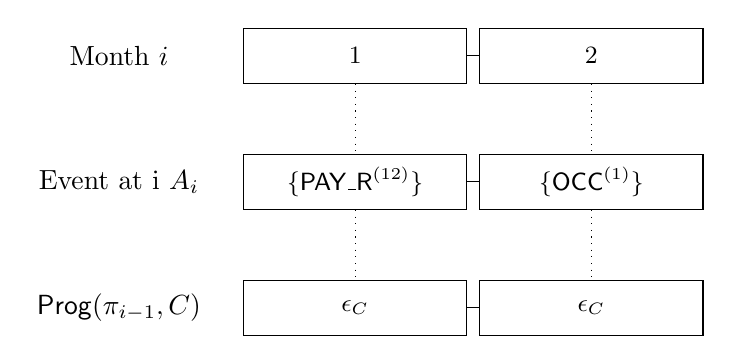
\begin{tikzpicture}[y=1.6cm,x=3.0cm]
    
      \tikzset{
        cell/.style={
          draw, rectangle, text width=26mm,
          minimum height=7mm, align=center, font=\small
        }
      }
    
      % Labels
      \node at (0,0)   {Month $i$};
      \node at (0,-1)  {Event at i $A_i$};
      \node at (0,-2)  {$\Prog(\pi_{i-1},C)$};
      % Row 1: time
      \node[cell] at (1,0) (t1) {$1$};
      \node[cell] at (2,0) (t2) {$2$};
      % Row 2: events
      \node[cell] at (1,-1) (e1) {$\{\PAY^{(12)}\}$};
      \node[cell] at (2,-1) (e2) {$\{\OCC^{(1)}\}$};
      % Row 3: residuals
      \node[cell] at (1,-2) (r1) {\emptc};
      \node[cell] at (2,-2) (r2) {\emptc};
      % Arrows
      \draw (t1)--(t2);
      \draw (e1)--(e2);
      \draw (r1)--(r2);
      % Vertical alignment
      \draw[dotted](t1.south)--(e1.north);
      \draw[dotted](e1.south)--(r1.north);
    
      \draw[dotted](t2.south)--(e2.north);
      \draw[dotted](e2.south)--(r2.north);
    \end{tikzpicture}
    }}
    {Progression on $ \obl[1]{\PAY}\ \repair\ \obl[1]{\PAYF}$ with a trace for which a no reparation is not required}
    {example:prog-repair1}
    {\vspace{8pt}}{\vspace{-12pt}}

\medskip
\noindent\textbf{Scenario 2: Violation and Repair.}
In trace $\pi'$, the tenant fails to pay in Month 1 ($\PAY \notin A'_1$). Here, $\trace{A'_1} \violt \obl[1]{\PAY}$. Consequently, the CPM activates the repair branch. The residual for Month 2 becomes $\obl[1]{\PAYF}$, obliging the tenant to pay the fine.

  \boxalignfigure{\resizebox{0.7\textwidth}{!}{%
  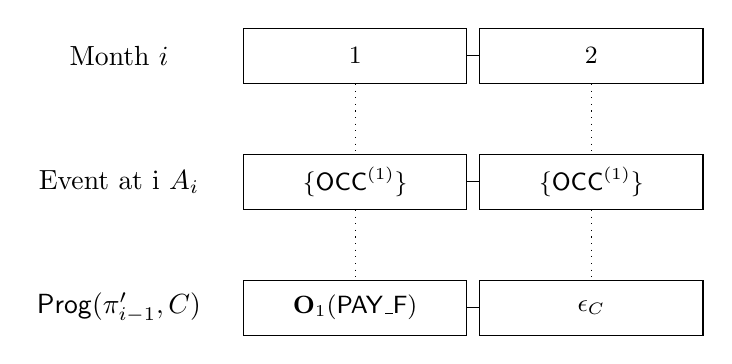
\begin{tikzpicture}[y=1.6cm,x=3.0cm]
  
    \tikzset{
      cell/.style={
        draw, rectangle, text width=26mm,
        minimum height=7mm, align=center, font=\small
      }
    }
  
    % Labels
    \node at (0,0)   {Month $i$};
    \node at (0,-1)  {Event at i $A_i$};
    \node at (0,-2)  {$\Prog(\pi'_{i-1},C)$};
    % Row 1: time
    \node[cell] at (1,0) (t1) {$1$};
    \node[cell] at (2,0) (t2) {$2$};
    % Row 2: events
    \node[cell] at (1,-1) (e1) {$\{\OCC^{(1)}\}$};
    \node[cell] at (2,-1) (e2) {$\{\OCC^{(1)}\}$};
    % Row 3: residuals
    \node[cell] at (1,-2) (r1) {$\obl[1]{\PAYF}$};
    \node[cell] at (2,-2) (r2) {\emptc};
    % Arrows
    \draw (t1)--(t2);
    \draw (e1)--(e2);
    \draw (r1)--(r2);
  
    % Vertical alignment
    \draw[dotted](t1.south)--(e1.north);
    \draw[dotted](e1.south)--(r1.north);
  
    \draw[dotted](t2.south)--(e2.north);
    \draw[dotted](e2.south)--(r2.north);
  
  \end{tikzpicture}
  }}
  {Progression on $ \obl[1]{\PAY}\ \repair\ \obl[1]{\PAYF}$ with a trace for which a no reparation is not required}
  {example:prog-repair2}
  {\vspace{8pt}}{\vspace{-12pt}}
\end{example}

Having established how single-step reparations evolve, we now extend the analysis to ongoing contracts. The following example demonstrates how the CPM handles infinite streams where duties recur every month, showing how violations in one period persist into the next.

\begin{example}[Progression of Infinite Repetition]
Consider the recurring contract $\repit{C_3}$, where the tenant must pay rent (or a fine) every month.
\[ \repit{C_3} = \repit{ \obl[1]{\PAY}\ \repair\ \obl[1]{\PAYF}}. \]

\noindent\textbf{Trace Analysis.}
We observe a trace where the tenant pays in Month 1 but fails to pay in Month 2 (occupying instead).
\begin{itemize}
    \item \textbf{Step 1 ($A_1$):} The tenant pays. The instance of $C_3$ for Month 1 is discharged. Due to the repetition operator, the residual is $\emptc ; \repit{C_3} \equiv \repit{C_3}$. The contract effectively ``resets'' for the next month.
    \item \textbf{Step 2 ($A_2$):} The tenant occupies but does not pay. The instance of $C_3$ for Month 2 is violated. Unlike Step 1, the residual does not reset cleanly. Instead, the violated obligation transforms into its reparation $\obl[1]{\PAYF}$, which must be fulfilled in the \emph{next} step (Month 3), alongside the continuing repetition $\repit{C_3}$.
\end{itemize}
This results in an accumulation of duties: the fine from Month 2 and the new rent for Month 3.

  \boxalignfigure{\resizebox{0.7\textwidth}{!}{%
  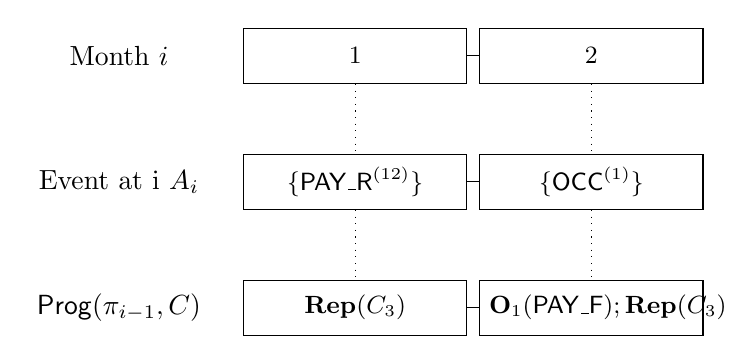
\begin{tikzpicture}[y=1.6cm,x=3.0cm]
  
    \tikzset{
      cell/.style={
        draw, rectangle, text width=26mm,
        minimum height=7mm, align=center, font=\small
      }
    }
  
    % Labels
    \node at (0,0)   {Month $i$};
    \node at (0,-1)  {Event at i $A_i$};
    \node at (0,-2)  {$\Prog(\pi_{i-1},C)$};
    % Row 1: time
    \node[cell] at (1,0) (t1) {$1$};
    \node[cell] at (2,0) (t2) {$2$};
    % Row 2: events
    \node[cell] at (1,-1) (e1) {$\{\PAY^{(12)}\}$};
    \node[cell] at (2,-1) (e2) {$\{\OCC^{(1)}\}$};
    % Row 3: residuals
    \node[cell] at (1,-2) (r1) {$\repit{C_3}$};
    \node[cell] at (2,-2) (r2) {$\obl[1]{\PAYF} ; \repit{C_3}$};
    % Arrows
    \draw (t1)--(t2);
    \draw (e1)--(e2);
    \draw (r1)--(r2);
  
    % Vertical alignment
    \draw[dotted](t1.south)--(e1.north);
    \draw[dotted](e1.south)--(r1.north);
  
    \draw[dotted](t2.south)--(e2.north);
    \draw[dotted](e2.south)--(r2.north);
  
  \end{tikzpicture}
  }}
  {Progression on $\repit{C_3}$ where the obligation is met in the first month but violated in the second.}
  {example:prog-repitc1}
  {\vspace{8pt}}{\vspace{-12pt}}
\end{example}

While repetitions capture simple recurring duties, more complex contracts are often bounded by conditions. Finally, we examine how the CPM handles \emph{guarded contracts}, where the outer structure (the guard) and the inner structure (the obligations) evolve independently until a termination event occurs.

\begin{example}[Progression of Guarded Contracts]
We examine a guarded contract that persists until a termination notice ($\notifterm$) is issued.
\[ \guard[\Gamma^+ \cdot \notifterm^{(1)}]{\repit{C_3}} \]

\noindent\textbf{Trace 1: Successful Termination.}
The tenant pays in Month 1 ($A_1$) and issues a termination notice in Month 2 ($A_2$).
\begin{itemize}
    \item At $i=1$, the event $A_1$ satisfies the inner contract $C_3$ (rent paid), but does not satisfy the guard (no notice). The residual is the guarded repetition.
    \item At $i=2$, the event $A_2$ contains $\notifterm$. This satisfies the guard expression. The CPM immediately reduces the entire contract to $\emptc$, signifying the contract has ended.
\end{itemize}

  \boxalignfigure{\resizebox{0.85\textwidth}{!}{%
  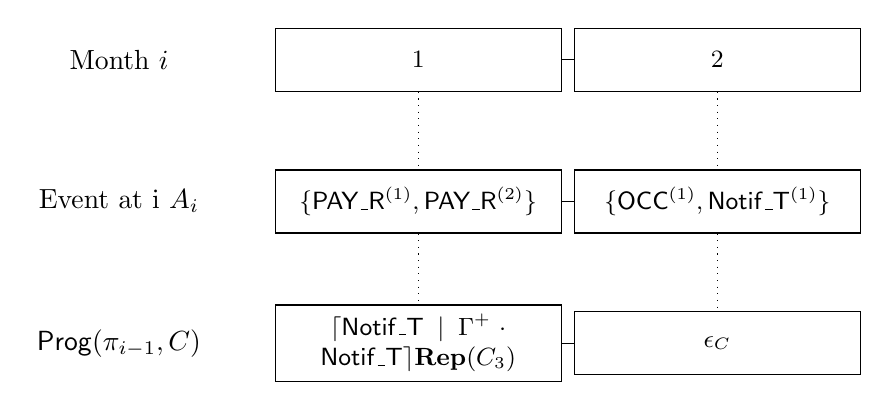
\begin{tikzpicture}[y=1.8cm,x=3.8cm]
  
    \tikzset{
      cell/.style={
        draw, rectangle, text width=34mm,
        minimum height=8mm, align=center, font=\small
      }
    }
    % Local definition for the residual regex to fit in the box
    \def\resid{\notifterm \mid \Gamma^+ \cdot \notifterm}
  
    % Labels
    \node at (0,0)   {Month $i$};
    \node at (0,-1)  {Event at i $A_i$};
    \node at (0,-2)  {$\Prog(\pi_{i-1},C)$};
    % Row 1: time
    \node[cell] at (1,0) (t1) {$1$};
    \node[cell] at (2,0) (t2) {$2$};
    % Row 2: events
    \node[cell] at (1,-1) (e1) {$\{\PAY^{(1)}, \PAY^{(2)}\}$};
    \node[cell] at (2,-1) (e2) {$\{\OCC^{(1)}, \notifterm^{(1)}\}$};
    % Row 3: residuals
    % Step 1: Contract satisfied (payment made), Guard not satisfied yet (needs >0 length or specific event).
    % Residual guard becomes (Notif | Gamma+ . Notif)
    \node[cell] at (1,-2) (r1) {$\guard[\resid]{\repit{C_3}}$};
    % Step 2: Guard satisfied by NotifTerm in A2. Contract discharges to epsilon.
    \node[cell] at (2,-2) (r2) {\emptc};
    % Arrows
    \draw (t1)--(t2);
    \draw (e1)--(e2);
    \draw (r1)--(r2);
  
    % Vertical alignment
    \draw[dotted](t1.south)--(e1.north);
    \draw[dotted](e1.south)--(r1.north);
  
    \draw[dotted](t2.south)--(e2.north);
    \draw[dotted](e2.south)--(r2.north);
  
  \end{tikzpicture}
  }}
  {Progression on guarded contract where the termination notice at step 2 discharges the contract.}
  {example:prog-guard1}
  {\vspace{8pt}}{\vspace{-12pt}}

\medskip
\noindent\textbf{Trace 2: Pending Guard with Internal Violation.}
In this scenario, the tenant pays in Month 1 but fails to pay (and gives no notice) in Month 2.
\begin{itemize}
    \item At $i=2$, the guard is \emph{not} satisfied.
    \item Simultaneously, the inner contract $\repit{C_3}$ processes the event. Since rent was not paid, the inner contract evolves into a reparation state ($\obl[1]{\PAYF}$).
    \item The resulting residual is a guarded reparation: $\guard[\dots]{(\obl[1]{\PAYF} ; \repit{C_3})}$.
\end{itemize}
This illustrates how the CPM maintains the ``wrapper'' (the guard) while the content inside (the obligations) evolves and accumulates violations independently.

  \boxalignfigure{\resizebox{0.95\textwidth}{!}{%
  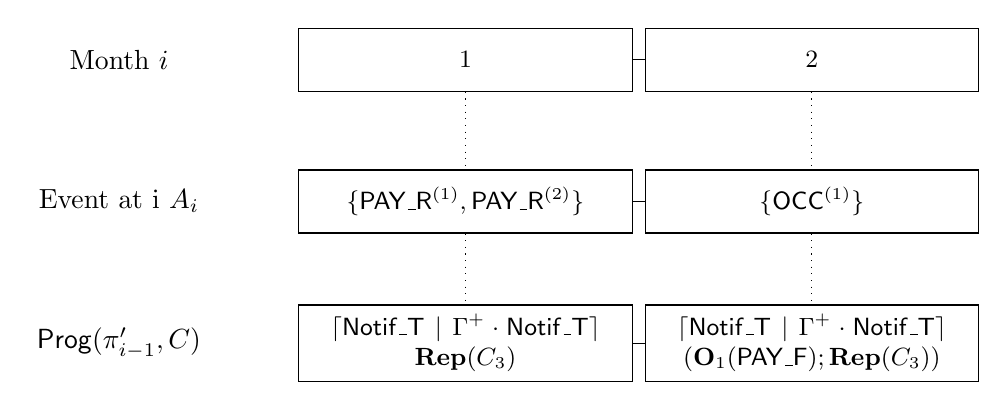
\begin{tikzpicture}[y=1.8cm,x=4.4cm]
  
    \tikzset{
      cell/.style={
        draw, rectangle, text width=40mm,
        minimum height=8mm, align=center, font=\small
      }
    }
    \def\resid{\notifterm \mid \Gamma^+ \cdot \notifterm}
  
    % Labels
    \node at (0,0)   {Month $i$};
    \node at (0,-1)  {Event at i $A_i$};
    \node at (0,-2)  {$\Prog(\pi'_{i-1},C)$};
    
    % Row 1: time
    \node[cell] at (1,0) (t1) {$1$};
    \node[cell] at (2,0) (t2) {$2$};
    
    % Row 2: events
    \node[cell] at (1,-1) (e1) {$\{\PAY^{(1)}, \PAY^{(2)}\}$};
    \node[cell] at (2,-1) (e2) {$\{\OCC^{(1)}\}$};
    
    % Row 3: residuals
    % Step 1: Manual line break using \\
    \node[cell] at (1,-2) (r1) {$\lceil \resid \rceil$ \\ $\repit{C_3}$};
    % Step 2: Manual line break using \\
    \node[cell] at (2,-2) (r2) {$\lceil \resid \rceil$ \\ $(\obl[1]{\PAYF} ; \repit{C_3})$};
    % Arrows
    \draw (t1)--(t2);
    \draw (e1)--(e2);
    \draw (r1)--(r2);
  
    % Vertical alignment
    \draw[dotted](t1.south)--(e1.north);
    \draw[dotted](e1.south)--(r1.north);
  
    \draw[dotted](t2.south)--(e2.north);
    \draw[dotted](e2.south)--(r2.north);
  
  \end{tikzpicture}
  }}
  {Progression on guarded contract where the guard is not satisfied and the inner contract triggers a reparation.}
  {example:prog-guard2}
  {\vspace{8pt}}{\vspace{-12pt}}
  
\end{example}


\section{Quantative violation semantics}
To define the quantitative violation semantics to not stop at the first violation prefix, we reuse  \emph{Contract Progress function} as the underlying state-transition mechanism.
 The progression function $\Prog$ is utilized to dynamically evolve the contract after every observation, producing a sequence of \emph{residual contracts} that represent the exact normative state at each point in time.
  By updating the contract state step-by-step, we ensure that the violation score for any given event is calculated strictly against the specific literals in force at that moment, accounting for all prior satisfactions, discharges, or triggered reparations. Then propagating the updated residual to the subsequent evaluation step.
  \begin{definition}[Quantitative Violation Semantics]
    Let $\trace{A}$ be a single event trace over $\Gamma$,  $\pi$ be a (possibly empty) finite trace $\Gamma^*$, and $C$ be a contract from $\cDL$.
    We define the \emph{quantitative violation semantics}, denoted by $\qsem{}: \Gamma^*, \cDL \to \mathbb{N} $, which maps a trace and a contract to a  natural number representing the violation score of trace on the contract. 
    The function is defined recursively by evaluating the head of the trace ($\trace{A}$) and propagating the residual contract to the tail ($\pi$):
    \[
    \qsem{\trace{A}\concat \pi, C} :=
    \begin{cases} 
      \qsem{\trace{A}, C } & \text{if } \pi = \epsilon \lor \Prog(\trace{A},C)= \emptc,\\
      \qsem{\trace{A}, C } + \qsem{\pi, \Prog(\trace{A},C)} & \text{otherwise}.
    \end{cases}
    \]
    where the \emph{instantaneous violation score} for a single event $\trace{A}$ against a contract $C$ is defined inductively on the structure of the contract:
    \[
    \qsem{\trace{A}, C} :=
    \begin{cases} 
      \qsem{\trace{A}, C_1 } + \qsem{\trace{A}, C_2} & \text{if } C = C_1 \wedge C_2, \\
      1 & \text{if } \trace{A} \violt C, \\
      0 & \text{otherwise}.
    \end{cases}
    \]
    \end{definition}
Intuitively, the formula $\qsem{\trace{A}\concat \pi, C}$ treats the contract execution as a path-accumulation problem. At every time step, the function:
\begin{enumerate}
    \item \textbf{Snapshots the penalty:} It calculates $\qsem{\trace{A}, C}$, which asks ``Given the current literals from$C$, does the current event $A$ violate any of them?'' This is a stateless check based purely on the structure of $C$ at that instant.
    \item \textbf{Updates the state:} It computes $\Prog(\trace{A}, C)$, effectively moving the contract pointer forward (e.g., from a paid obligation to the next month's rent, or from a violated duty to a reparation).
    \item \textbf{Accumulates:} It adds the snapshot penalty to the result of the recursive call on the remaining trace using the \emph{new} state.
\end{enumerate}

Intuitively, the formula $\qsem{\trace{A}\concat \pi, C}$ treats the contract execution as a path-accumulation problem. At every time step, the function:
\begin{enumerate}
    \item \textbf{Snapshots the penalty:} It calculates $\qsem{\trace{A}, C}$, which asks ``Given the current literals from $C$, does the current event $A$ violate any of them?'' This is a stateless check based purely on the structure of $C$ at that instant.
    \item \textbf{Updates the state:} It computes $\Prog(\trace{A}, C)$, effectively moving the contract pointer forward (e.g., from a paid obligation to the next month's rent, or from a violated duty to a reparation).
    \item \textbf{Accumulates:} It adds the snapshot penalty to the result of the recursive call on the remaining trace using the \emph{new} state.
\end{enumerate}

The explicit handling of Sequence and Reparation is done in the contract progress function, which ensures that ``zero-delay'' transitions are penalized correctly. For instance, if a contract requires $C_1$ then $C_2$, and an event discharges $C_1$ but violates $C_2$ in the same step, the summation logic ($\qsem{\trace{A}, C_1} + \qsem{\trace{A}, C_2}$) ensures the violation of $C_2$ is not ignored simply because it appeared in a continuation.


The definition of the instantaneous score $\qsem{\trace{A}, C}$ rests on distinguishing between \textbf{concurrent} (parallel) obligations and \textbf{structural} (atomic) constraints. It decouples the measurement of the ``volume'' of non-compliance from the binary verification of specific rules.

\paragraph{Additivity of Concurrency.}
The case $\qsem{\trace{A}, C_1 \wedge C_2} := \qsem{\trace{A}, C_1 } + \qsem{\trace{A}, C_2}$ captures the ``width'' of the violation as show in Example.\ref{fig:joint-blame}. In normative systems, a conjunction represents distinct, independent obligations active simultaneously. By summing the scores, the function ensures that the penalty is proportional to the number of distinct parallel duties neglected in a single instant, preventing ``violation masking'' where a single boolean verdict would hide multiple breaches.

\paragraph{Binary Structural Verdict.}
For constructs that are not distinct parallel duties (such as literals, sequences, or reparations), the definition relies on the binary tight violation relation ($\violt$). This captures the ``existence'' of a fault in a non-decomposable structure. For example, a single atomic duty ($\obl{a}$) can only be violated once per step.

\paragraph{Separation of State and Score.}
This approach assumes that the complexity of temporal evolution is handled by $\Prog$, while $\qsem{}$ handles the instantaneous cost. By reducing non-conjunction cases to a simple check ($\trace{A} \violt C$), the definition asserts that scoring is local (checking if the current active node is broken), while progression is temporal (handling the flow from one obligation to the next).

We summarize these properties in the following theorem, which establishes that the quantitative score is a monotonically increasing function that acts as a "super-set" of the binary violation semantics.
While a binary trace might be "Satisfied" (via reparation), the quantitative score reveals the cost of that path.

\subsection{Formal Correspondence between Tight and Quantitative Semantics}

The quantitative semantics presented above is not an arbitrary metric but a consistent extension of the forward-looking tight semantics.
While tight semantics provides a binary decisive verdict (satisfaction vs.\ violation), the quantitative semantics provides a cumulative measure of deviation.
We now establish the formal link between these two frameworks through the properties of \emph{Score Stability} and \emph{Violation Detection}.

The first connection concerns the relationship between the discharge of a contract (reaching $\emptc$) and the tight satisfaction relation $\satt$.
When a contract is tightly satisfied, it conceptually ceases to impose new requirements.
The progression function reflects this by transitioning to the neutral element $\emptc$.

\begin{lemma}[Satisfaction Saturation]
\label{lem:sat-saturation}
Let $C$ be a contract and $\pi$ be a finite trace.
If the contract is tightly satisfied by $\pi$, the progression function reduces to the empty contract, and the cumulative violation score stabilizes.
Formally:
\[
\pi \satt C \implies \Prog(\pi, C) = \emptc.
\]
Consequently, for any extension $\pi'$ of $\pi$:
\[
\qsem{\pi \concat \pi', C} = \qsem{\pi, C}.
\]
\end{lemma}

\begin{proof}
The proof follows from the definition of $\Prog$.
For every construct (Literal, Reparation, Guard, Trigger), the progression function is defined to return $\emptc$ exactly when the condition $\trace{A} \satt C$ is met.
Since $\qsem{\trace{A}, \emptc} = 0$ for any event $A$, no further penalties can be accumulated once the residual contract becomes $\emptc$.
\end{proof}

The second connection concerns the relationship between tight violations and the instantaneous score.
A key feature of the quantitative semantics is that it is strictly stricter than the binary semantics: it assigns a positive penalty to \emph{every} tight violation, even those that are subsequently repaired.

\begin{lemma}[Positive Penalty for Tight Violation]
\label{lem:violation-penalty}
Let $C$ be a contract and $\trace{A}$ be a single event.
If the event tightly violates the contract, the instantaneous violation score is strictly positive.
\[
\trace{A} \violt C \implies \qsem{\trace{A}, C} \ge 1.
\]
\end{lemma}

\begin{proof}
We proceed by structural induction on $C$.
\begin{itemize}
    \item \textbf{Base Case (Literals):} If $\trace{A} \violt \ell$, then by definition $\qsem{\trace{A}, \ell} = 1$.
    \item \textbf{Conjunction ($C_1 \wedge C_2$):} By Definition~\ref{def:binary-contract-semantics}, $\trace{A} \violt C_1 \wedge C_2$ implies $\trace{A} \violt C_1$ or $\trace{A} \violt C_2$.
    Consequently, $\qsem{\trace{A}, C_1} \ge 1$ or $\qsem{\trace{A}, C_2} \ge 1$. Since the score is additive ($\qsem{\trace{A}, C_1} + \qsem{\trace{A}, C_2}$), the total is $\ge 1$.
    \item \textbf{Reparation ($C_1 \repair C_2$):} $\trace{A} \violt C_1 \repair C_2$ implies $\trace{A} \violt C_1$ and $\trace{A} \violt C_2$.
    The scoring function sums violations of $C_1$ (score 1) and $C_2$. Thus, the score is at least 1.
\end{itemize}
The sequence case follows similarly via the immediate handover logic.
\end{proof}

We summarize these properties in the following theorem, which establishes that the quantitative score is a monotonically increasing function that acts as a "super-set" of the binary violation semantics.
While a binary trace might be "Satisfied" (via reparation), the quantitative score reveals the cost of that path.


\begin{theorem}[Consistency of Quantitative and Tight Semantics]
  \label{thm:quant-consistency}
  For any contract $C$ and finite trace $\pi$:
  \begin{enumerate}
      \item \textbf{Zero Score Implications:}
      If $\qsem{\pi, C} = 0$, then exactly one of the following three disjoint cases holds:
      \begin{enumerate}
        \item $\pi \satt C$ if and only if $\Prog(\pi, C) = \emptc$ and $\forall k < |\pi|-1:\Prog(\pi[0,k], C) \neq \emptc$.
        \item $\pi \postsat C$ if and only if $\Prog(\pi, C) = \emptc$ and\\ $\exists k < |\pi|-1$ such that $\Prog(\pi[0,k], C) = \emptc$.
        \item $\pi \presat C$ if and only if $\Prog(\pi, C) \neq \emptc$.
      \end{enumerate}
      
      \item \textbf{Non-Zero Score Implications:}
      If $\qsem{\pi, C} \neq 0$, then:
      \begin{enumerate}
        \item $\pi \violt C$ if and only if $\qsem{\pi, C} = 1$ and $\qsem{\pi[0, |\pi|-2], C} = 0$.
        \item $\pi \postviol C$ if and only if $\qsem{\pi, C} > 1$ or ($\qsem{\pi, C} = 1$ and\\ $\qsem{\pi[0, |\pi|-2], C} = 1$).
      \end{enumerate}
      
      \item \textbf{Reparation Cost:}
      If $\pi$ satisfies $C$ strictly through a reparation mechanism (i.e., $\pi \satt C$ but primary obligations failed), then $\qsem{\pi, C} > 0$.
  \end{enumerate}
  \end{theorem}
  
  \begin{proof}
  We prove the implications by structural induction on the trace $\pi$ and the contract $C$, utilizing the definitions of the quantitative function $\qsem{}$ and the contract progression $\Prog$.
  
  \paragraph{1. Zero Score Implications ($\qsem{\pi, C} = 0$)}
  Assume $\qsem{\pi, C} = 0$. By the definition of the cumulative score, this implies that for all steps $i < |\pi|$, the instantaneous penalty is zero: $\qsem(\trace{A_i}, C_i) = 0$. Consequently, no tight violation has occurred at any step. The contract state evolves purely via $\Prog$ without triggering any penalty clauses.
  
  \begin{enumerate}
      \item \textbf{Case 1(a): Tight Satisfaction ($\satt$).}
      \begin{itemize}
          \item $(\Rightarrow)$ Assume $\Prog(\pi, C) = \emptc$ and for all strict prefixes $\pi'$, $\Prog(\pi', C) \neq \emptc$.
          The condition $\Prog(\pi, C) = \emptc$ indicates that the contract has been fully discharged. Since the score is 0, this discharge was not achieved via a violation-triggered path (e.g., a reparation where the primary failed). The absence of $\emptc$ in prior prefixes ensures that this is the \emph{first} moment of discharge. By Definition~\ref{def:binary-contract-semantics} (Tight Satisfaction), the first prefix to fully satisfy the obligations corresponds to $\satt$.
          \item $(\Leftarrow)$ If $\pi \satt C$, then by Lemma~\ref{lem:sat-saturation} (Satisfaction Saturation), the progression must reach $\emptc$ exactly at $\pi$. Since it is a \emph{tight} satisfaction, no proper prefix could have satisfied it (reached $\emptc$) earlier.
      \end{itemize}
  
      \item \textbf{Case 1(b): Post Satisfaction ($\postsat$).}
      \begin{itemize}
          \item The condition $\exists k < |\pi|$ such that $\Prog(\pi[0,k], C) = \emptc$ implies that the contract was already discharged at a previous step $k$.
          \item By Definition~\ref{def:postprecont}, $\pi \postsat C$ holds if there exists a strict prefix that tightly satisfies $C$. Since the score is 0, the path to $k$ was compliant. Thus, the state remains $\emptc$ for the remainder of the trace, maintaining the $\postsat$ status.
      \end{itemize}
  
      \item \textbf{Case 1(c): Pre Satisfaction ($\presat$).}
      \begin{itemize}
          \item Assume $\Prog(\pi, C) \neq \emptc$. Since $\qsem{\pi, C} = 0$, no violation has occurred. However, the contract has not reduced to the empty contract $\emptc$, meaning active obligations remain.
          \item This satisfies the definition of $\presat$: the trace is neither satisfied ($\satt/\postsat$) nor violated ($\violt/\postviol$). It is effectively "pending."
      \end{itemize}
  \end{enumerate}
  
  \paragraph{2. Non-Zero Score Implications ($\qsem{\pi, C} \neq 0$)}
  Assume $\qsem{\pi, C} > 0$. This implies $\exists i$ such that $\qsem(\trace{A_i}, C_i) > 0$.
  
  \begin{enumerate}
      \item \textbf{Case 2(a): Tight Violation ($\violt$).}
      \begin{itemize}
          \item We consider the case where $\qsem{\pi, C} = 1$, the score of the immediate prefix is $0$ and let $n= \size{\pi}$ .
          \item $\qsem{\pi[0..n-2], C} = 0$ implies that for all previous steps, the contract was in a compliant state ($\presat$).
          \item The jump to $\qsem{\pi, C} = 1$ implies that the instantaneous score at the last step $\qsem{\trace{A_{n-1}}, \Prog(\pi[0,n-2],C)} = 1$.
          \item By Lemma~\ref{lem:violation-penalty}, a positive instantaneous score corresponds to a tight violation of the active residual contract.
          \item Since this is the \emph{first} non-zero score, it corresponds to the \emph{first} prefix that triggers a violation. This matches the definition of $\pi \violt C$.
      \end{itemize}
  
      \item \textbf{Case 2(b): Post Violation ($\postviol$).}
      \begin{itemize}
          \item The condition $\qsem{\pi, C} > 1$ or ($\qsem{\pi, C}=1$ and $\qsem{prefix}=1$) implies that the violation score did not originate purely at the current step (or if it did, it was cumulative).
          \item Specifically, if $\qsem{\pi[0..n-2], C} \ge 1$, then a violation occurred strictly in the past.
          \item By Definition~\ref{def:postprecont}, if a strict prefix tightly violated the contract ($\violt$), the current trace is in $\postviol$. The non-zero score is carried forward monotonically.
      \end{itemize}
  
      \item \textbf{Case 2(c): Reparation Cost.}
      \begin{itemize}
          \item Consider a contract $C_{primary} \repair C_{repair}$.
          \item If $\pi$ satisfies this strictly through the reparation mechanism, it means $\pi$ did \emph{not} satisfy $C_{primary}$.
          \item By the definition of reparation progression, the transition to $C_{repair}$ occurs only if $\pi \violt C_{primary}$.
          \item By the definition of the instantaneous scoring function for reparation,\\ $\qsem{\trace{A}, C_{primary} \repair C_{repair}} = 1 + \dots$ when the primary violates.
      \end{itemize}
      Therefore, the path involving the repair accumulates a score of at least 1 (the penalty for breaking the primary), confirming $\qsem{\pi, C} > 0$.
  \end{enumerate}
  \end{proof}

This theorem highlights the utility of the quantitative approach for post-hoc analysis: distinguishing between a "perfect" execution (Score 0) and a "compliant but costly" execution (Score $>0$, e.g., paying fines), a distinction lost in the binary $\satt$ verdict.





\bibliographystyle{plain}   % or any style you prefer, like 'abbrv' or 'apalike'
\bibliography{bibd}
\end{document}
